\documentclass{article}
\usepackage[letterpaper, left=3.75cm, right=3.75cm, top=2.5cm,
bottom=2.5cm,dvips]{geometry}
\usepackage[utf8]{inputenc}
\usepackage[italian]{babel}
\usepackage{gensymb}
\usepackage{amsmath}
\usepackage{amssymb}
\usepackage{wrapfig}
\usepackage{graphicx}
\usepackage{setspace} \doublespacing
\usepackage{hyperref}
\usepackage{listings}
\usepackage{xcolor}
\usepackage{empheq}
\usepackage{amsfonts}
\usepackage{marvosym }
\usepackage{MnSymbol}
\usepackage{esint}
%\usepackage[margin=4cm]{geometry}
\usepackage[most]{tcolorbox}
\newcommand{\R}{\mathbb{R}}
\newcommand{\C}{\mathbb{C}}
\newcommand{\Z}{\mathbb{Z}}
\newcommand{\Q}{\mathbb{Q}}
\newcommand{\N}{\mathbb{N}}
\newcommand{\Ln}{\text{Ln}}
\newcommand{\sgn}{\text{sgn}}
\newcommand{\dom}{\text{dom}}
\hypersetup{
    colorlinks=true,
    linkcolor=red,
    filecolor=magenta,      
    urlcolor=red,
    }

\title{Appunti di Analisi 2}
\author{Giacomo Veglio}
\date{Febbraio 2022}

\begin{document}
\begin{titlepage}
    \begin{center}
        
        \Large\textbf{Università di Padova} \\
        \large\textbf{Dipartimento di Fisica e Astronomia “Galileo Galilei”}\\
        \textbf{Anno accademico:} 2022-23\\
        \vspace{30pt}
        
\includegraphics[width=0.4\textwidth]{UniPdlogo.png}
        \hspace{30pt}
        
\includegraphics[width=0.4\textwidth]{DFALogo.jpg}\\
        \vspace{30pt} \hline
        \vspace{15pt}
        \large\textbf{Appunti delle Lezioni di Analisi 2 del Prof. Marson}\\
        \vspace{15pt}
        \hline
        \vspace{30pt}
        \textbf{Giacomo Veglio}\\
        \vspace{15pt}
        \textbf{La\TeX}\\
        \vspace{15pt}
        \textbf{Data:} 27/02/2023\\
        \vspace{15pt}
        \begin{figure}[h!]
            \centering
            
\includegraphics[width=0.5\textwidth]{tuxflag.png}
        \end{figure}
    \end{center}
\end{titlepage}

\renewcommand{\contentsname}{Indice}
\tableofcontents
\newpage

\section{\textcolor{red}{Lezione 1 \space\space 27/02/'23}}
\subsection{\textcolor{red}{Serie Numeriche}}
\paragraph{}
    \begin{empheq}{align*}
        sin(x)&=\sum_{k=0}^{\infty} (-1)^k \frac{x^{2k+1}}{(2k+1)!}\\
        sin(4)&=\sum_{k=0}^{\infty} (-1)^k \frac{4^{2k+1}}{(2k+1)!}= 4-\frac{4^3}{3!}+\frac{4^5}{5!}-\frac{4^7}{7!}+...\\
        \sum_{k=1}^{\infty} \frac{1}{k}&= 1+\frac{1}{2}+\frac{1}{3}+\frac{1}{4}+\frac{1}{5}=+\infty
    \end{empheq}
Sappiamo solo sommare un numero finito di addendi!
    \begin{empheq}{align}
        \nonumber &\sum_{k=1}^{5} \frac{1}{k}= 1+\frac{1}{2}+\frac{1}{3}+\frac{1}{4}+\frac{1}{5}\\
        \nonumber &\sum_{k=1}^{10} \frac{1}{k}= 1+\frac{1}{2}+\frac{1}{3}+...+\frac{1}{10}
    \end{empheq}
Per $n\geq 1$ possiamo però ricavarci i limiti ad infinito di una serie.
    \begin{empheq}{equation*}
        \sum_{k=1}^{n} \frac{1}{k}= 1+\frac{1}{2}+\frac{1}{3}+...+\frac{1}{n} \Longrightarrow \sum_{k=1}^{\infty} \frac{1}{k} = \lim_{n\rightarrow +\infty} \sum_{k=1}^{n} \frac{1}{k}
    \end{empheq}

\paragraph{\textcolor{red}{Definizione}}
Una serie a valori in $\C$ è una coppia $( \{a_n \}_{n\in \N},\{S_n\}_{n\in \N})$ tale che $\{a_n \}_{n\in \N}\subseteq \C$ è una successione e $\{S_n\}_{n\in \N}$ è la sua successione delle ridotte n-esima,
\begin{empheq}{align}
    \nonumber S_n &= \sum_{k=0}^{n} a_k.\\
    \nonumber S_0 &=a_0\\
    \nonumber S_1 &=a_0+a_1\\
    \nonumber S_2 &=a_0+a_1+a_2\\
    \nonumber S_n &=a_0+a_1+a_2+...+a_n
\end{empheq}
La coppia $( \{a_n \}_{n\in \N},\{S_n\}_{n\in \N})$ è identificata con
\begin{empheq}{equation}
  \nonumber  \sum_{k=0}^{\infty} a_k.
\end{empheq}

\paragraph{\textcolor{red}{Definizione}}
Una serie $\sum_{k=0}^{\infty} a_k$ si dice
\begin{itemize}
    \item \textcolor{red}{Convergente} se converge la successione delle ridotte, cioè se $\exists$ finito 
            \begin{empheq}{equation}
                \nonumber \lim_{n\rightarrow +\infty} S_n = \lim_{n\rightarrow +\infty} \sum_{k=0}^{n} a_k
            \end{empheq}
    \item \textcolor{red}{Divergente}
        \begin{itemize}
            \item a $+\infty$ se $\lim_{n\rightarrow +\infty} S_n =+\infty$
            \item a $-\infty$ se $\lim_{n\rightarrow +\infty} S_n =-\infty$
            \item a $\infty$ se $\lim_{n\rightarrow +\infty} S_n =\infty$, cioè se $lim_{n\rightarrow +\infty} |S_n|=+\infty$
        \end{itemize}
    \item \textcolor{red}{Irregolare} o \textcolor{red}{indeterminata} se $\lim_{n\rightarrow +\infty} S_n$ non esiste.
\end{itemize}

\paragraph{\textcolor{red}{Esempio}}
    \begin{empheq}{align*}
        \sum_{k=0}^{\infty} (-1)^k \frac{4^{2k+1}}{(2k+1)!}=&\lim_{n\rightarrow +\infty} \sum_{k=0}^{n} (-1)^k \frac{4^{2k+1}}{(2k+1)!}=sin(4) \,\,\,\,\, \text{è convergente.}\\
        \sum_{k=1}^{\infty} \frac{1}{k} = &\lim_{n\rightarrow +\infty} \sum_{k=1}^{n} \frac{1}{k}=+\infty \,\,\,\,\, \text{ è divergente a} +\infty.
    \end{empheq}   
    
\paragraph{\textcolor{red}{Definizione}}
Se la serie $\sum_{k=0}^{\infty} a_k$ converge, cioè se il $\lim_{n\rightarrow +\infty} S_n = \lim_{n\rightarrow +\infty} \sum_{k=0}^{n} a_k$, si dice \textcolor{red}{somma della serie} ed è indicato con $\sum_{k=0}^{\infty} a_k$.

\paragraph{\textcolor{red}{Proposizione}}
Sia $\sum_{k=0}^{\infty} a_k$ una serie a termini complessi. Allora $\sum_{k=0}^{\infty} a_k$ converge $\Longleftrightarrow$ convergono $\sum_{k=0}^{\infty} Re(a_k)$ e $\sum_{k=0}^{\infty} Im(a_k)$
\begin{empheq}{equation*}
    a_k=\alpha_k +i\beta_k, \,\,\,\,\, \alpha_k,\beta_k \in \R
\end{empheq}
$\sum_{k=0}^{\infty} a_k$ converge $\Longleftrightarrow$ convergono entrambe le serie a termini in $\R$
\begin{empheq}{equation*}
    \sum_{k=0}^{\infty} \alpha_k \,\,\,\,\, \text{e} \,\,\,\,\, \sum_{k=0}^{\infty} \beta_k.
\end{empheq}

\paragraph{}
Delle serie è interessante studiare il \textcolor{red}{carattere}, cioè se convergono, divergono, o sono irregolari.

\paragraph{\textcolor{red}{Dimostrazione della proposizione $\Rightarrow)$}}    
    Se $\sum_{k=0}^{\infty} a_k$ converge allora $\sum_{k=0}^{\infty} \alpha_k$ e $\sum_{k=0}^{\infty} \beta_k$ convergono.\\
    Sia $S_a+iS_b$ la somma di $\sum_{k=0}^{\infty}a_k$, allora
    \begin{empheq}{equation*}
        S_a+iS_b=\lim_{n\rightarrow +\infty} \sum_{k=0}^{n} (\alpha_k + i\beta_k)
    \end{empheq}
    Faccio vedere che 
    \begin{empheq}{equation*}
        \lim_{n \rightarrow +\infty} \sum_{k=0}^{n}\alpha_k = S_a \,\,\,\,\, \text{e} \,\,\,\,\, \lim_{n \rightarrow +\infty} \sum_{k=0}^{n}\beta_k = S_b
    \end{empheq}
    allora
    \begin{empheq}{equation}
        \nonumber 0 \leq |\sum_{k=0}^{n} \alpha_k - S_a|=|Re(\sum_{k=0}^{n} a_k - (S_a +iS_b)|\leq |\sum_{k=0}^{n} a_k - (S_a +iS_b)| \xrightarrow{n\rightarrow +\infty} 0.
    \end{empheq}
Quindi per il Teorema dei Due Carabinieri
    \begin{empheq}{equation}
        \nonumber \lim_{n\rightarrow +\infty} |\sum_{k=0}^{n} \alpha_k - S_a|=0 \Longleftrightarrow \lim_{n\rightarrow +\infty} \sum_{k=0}^{n} \alpha_k =S_a
    \end{empheq}
In modo analogo si dimostra che $\lim_{n\rightarrow +\infty}\beta_k=S_b$
\begin{flushright}
\large\Lightning
\end{flushright}
\paragraph{\textcolor{red}{Dimostrazione della proposizione $\Leftarrow)$}}
\begin{empheq}{equation*}
    \sum_{k=0}^{\infty}\alpha_k \,\,\,\,\, \text{e} \,\,\,\,\, \sum_{k=0}^{\infty} \beta_k \,\,\,\,\, \text{convergono} \,\,\,\,\, \Longrightarrow \sum_{k=0}^{\infty} a_k \,\,\,\,\, \text{converge,}
\end{empheq}
 ovvero
\begin{empheq}{align}
    \nonumber \lim_{n\rightarrow +\infty} \sum_{k=0}^{n} \alpha_k &= S_a \in \R, \\
    \nonumber \lim_{n\rightarrow +\infty} \sum_{k=0}^{n} \beta_k &= S_b \in \R.
\end{empheq}
Quindi per $n\rightarrow +\infty$ si avrà la seguente disuguaglianza triangolare
\begin{empheq}{align*}
    0 \leq |\sum_{k=0}^{n} a_k& - (S_a +iS_b)| = |\left(\sum_{k=0}^{n} \alpha_k - S_a \right) + i\left(\sum_{k=0}^{n} \beta_k - S_b \right)| \leq \\ &\leq |\sum_{k=0}^{n} \alpha_k - S_a| - |\sum_{k=0}^{n} \beta_k -S_b| \xrightarrow{n \rightarrow +\infty} 0.
\end{empheq}
Si conclude con il Teorema dei Due Carabinieri.
\begin{flushright}
\large\Lightning
\end{flushright}

\newpage
\subsection{\textcolor{red}{"Paradosso" di Zenone}}
\paragraph{}
\begin{figure}[!h]
    \centering
    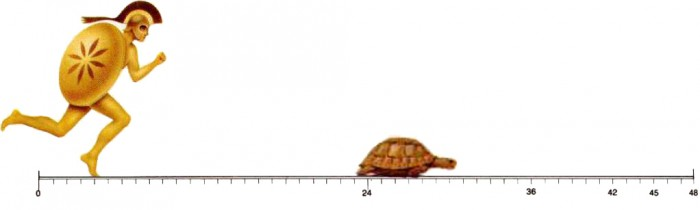
\includegraphics[width=\textwidth]{Zenone.jpg}
\end{figure}
\begin{center}
\begin{tabular}[!h]{c c | c}
    $L_0$ & $t_0=\frac{L_0}{v_A}$ & $L_1=t_0 v_T$\\
    $L_1$ & $t_1=\frac{L_1}{v_A}= t_0 \frac{v_T}{v_A}$ & $L_2=t_1 v_T$\\
    $L_2$ & $t_2=\frac{L_2}{v_A}=t_0 (\frac{v_T}{v_A})^2$ & $L_3=t_2 v_t$ \\
    $L_3$ & $t_3=\frac{L_3}{v_A}=t_0 (\frac{v_t}{v_A})^3$ & ...\\
\end{tabular}
\end{center}
Quanto tempo ci impiega Achille a raggiungere la tartaruga?
Se $v_T < v_A$ allora
\begin{empheq}{align}
    \nonumber T&=t_0 +t_1+t_2+...=\\
    \nonumber  &=t_0 \left(1+\frac{v_T}{v_A}+\left(\frac{v_T}{v_A}\right)^2+\left(\frac{v_T}{v_A}\right)^3+... \right)=\\
    \nonumber  &=t_0 \sum_{k=0}^{\infty} \left(\frac{v_T}{v_A}\right)^k = t_0 \frac{1}{1-\frac{v_T}{v_A}}=\frac{\frac{L_0}{v_A}}{1-\frac{v_T}{v_A}}
\end{empheq}
Osserviamo dunque che per una \textcolor{red}{serie quadratica} di \textcolor{red}{ragione} $r\in \C$ abbiamo 
\begin{empheq}{equation}
    \nonumber \sum_{k=0}^{\infty} r^k = r^0+r^1+r^2+...
\end{empheq}
Per $r=1$ avremo
\begin{empheq}{align}
    \nonumber \sum_{k=0}^{\infty} 1^k &=\lim_{n\rightarrow +\infty} \sum_{k=0}^{n} 1^k=\\
    \nonumber &=\lim_{n\rightarrow +\infty}(1+1+...+1)=\\
    \nonumber &=\lim_{n\rightarrow +\infty}(n+1)=+\infty.
\end{empheq}
Per $r\neq 1$ procuriamoci un'espressione della ridotta n-esima, cioè di
\begin{empheq}{align}
    \nonumber S_n &=\sum_{k=0}^{n} r^k = 1+r+r^2+...+r^n\\
    \nonumber S_{n+1}&=\sum_{k=0}^{n+1} r^k = 1+r+r^2+...+r^n+ r^{n+1}=\\
    \nonumber &=S_n + r^{n+1}=\\
    \nonumber &= 1+r(1+r+r^2+...+r^n)=\\
    \nonumber &=1+rS_n.
\end{empheq}
Dunque
\begin{empheq}{align}
    \nonumber S_n+r^{n+1}&=1+rS_n\\
    \nonumber S_n &=\frac{1-r^{n+1}}{1-r}.
\end{empheq}
Quindi avremo che $lim_{n\rightarrow +\infty} S_n = lim_{n \rightarrow +\infty} \frac{1-r^{n+1}}{1-r}$ \space $\exists$ finito e vale in tal caso $\frac{1}{1-r}\Leftrightarrow |r|<1$.\\
La serie geometrica di ragione $r$, $\sum_{k=0}^{\infty} r^k$ converge $\Leftrightarrow |r|<1$ e in tal caso la sua somma vale $\frac{1}{1-r}$.

\newpage
\section{\textcolor{red}{Lezione 2 \space\space 28/02/'23}}
\begin{empheq}{equation}
    \nonumber \sum_{k=0}^{\infty} r^k=\frac{1}{1-r} \Leftrightarrow |r|<1
\end{empheq}
\paragraph{\textcolor{red}{Esempio}}
Dimostriamo che $0.\overline{9} = 1$.
\begin{empheq}{align}
    \nonumber0.\overline{9}& =\sum_{k=1}^{\infty} \frac{9}{10^k}=\lim_{n \rightarrow +\infty} \sum_{k=1}^{n} \frac{9}{10^k}=\\
    \nonumber &=9\lim_{n\rightarrow +\infty} \sum_{k=1}^{n}\frac{1}{10^k}=\\
     \nonumber&= 9\lim_{n\rightarrow +\infty} \left(\sum_{k=1}^{n}\frac{1}{10^k}-\frac{1}{10^0}\right)=\\
     \nonumber&= 9\left(\sum_{k=1}^{\infty} \left( \frac{1}{10} \right)^k -1  \right)=9\left(\frac{1}{1-\frac{1}{10}}-1\right)=1
\end{empheq}

\subsection{\textcolor{red}{Serie telescopiche}}
\paragraph{}
\begin{empheq}{equation}
   \nonumber \sum_{k=0}^{\infty} [f(k+1)-f(k)], \space \space f:\N \rightarrow \C
\end{empheq}
Studiamo il carattere.
Procuriamoci, se possibile, l'espressione di una ridotta n-esima.
\begin{empheq}{align*}
    S_n=&\sum_{k=0}^{n}[f(k+1)-f(k)] =f(1)-f(0)+f(2)-f(1)+ \\
     & f(3)-f(2)+f(4)-f(3)+...+f(n+1)-f(n)=\\
     =&f(n+1)-f(0)
\end{empheq}
Avremo che 
\begin{empheq}{equation}
    \nonumber \exists \lim_{n\rightarrow +\infty} S_n =\lim_{n\rightarrow +\infty} [f(k+1)-f(k)] \Leftrightarrow \exists \lim_{n\rightarrow +\infty}f(n).
\end{empheq}
La serie converge $\Leftrightarrow \lim_{n\rightarrow +\infty}f(n)$ esiste finito e in tal caso la somma della serie è
\begin{empheq}{equation}
    \nonumber \sum_{k=0}^{\infty}[f(k+1)-f(k)]=\lim_{n \rightarrow +\infty} f(n)-f(0)
\end{empheq}

\paragraph{\textcolor{red}{Esempio: Serie di Mengoli}}
\begin{empheq}{equation}
    \nonumber \sum_{k=1}^{\infty} \frac{1}{k(k+1)} = \sum_{k=1}^{\infty} \left[ \frac{1}{k} - \frac{1}{k+1} \right]= -\sum_{k=1}^{\infty} \left[\frac{1}{k+1}-\frac{1}{k}\right]
\end{empheq}
Con $f(k)=\frac{1}{k}$ dunque
\begin{empheq}{equation}
    \nonumber \sum_{k=1}^{\infty} \frac{1}{k(k+1)} = -\lim_{n\rightarrow +\infty}[f(n)-f(1)]=f(1)=1
\end{empheq}

\subsection{\textcolor{red}{Studio del carattere di una serie}}
\paragraph{\textcolor{red}{Esempio}}
Studiamo il carattere della serie:
\begin{empheq}{align}
    \nonumber \sum_{k=0}^{\infty} cos(n \theta),\,\,\, \sum_{k=0}^{\infty} sin(n \theta),\,\,\, \theta \in [0, 2\pi].
\end{empheq}
Per la formula di Eulero ($e^{i\theta}=cos\theta+isin\theta$) abbiamo 
\begin{empheq}{equation}
    \nonumber e^{in\theta}=cos(n\theta)+isin(n\theta)  
\end{empheq}
\begin{empheq}{equation}
    \nonumber \sum_{n=0}^{\infty}[cos(n\theta)+isin(n\theta)]=\sum_{n=0}^{\infty}e^{in\theta}=\sum_{n=0}^{\infty}(e^{i\theta})^{n}
\end{empheq}
Non converge perchè è una serie geometrica di ragione $e^{i\theta}$ e $|e^{i\theta}|=1$. Per $n \neq 0,2\pi$ si ha
\begin{empheq}{align}
   \nonumber \sum_{n=0}^{n}cos(n\theta)&=Re\left( \sum_{k=0}^{n} \left( e^{i\theta} \right)^k \right)=\\
    \nonumber &=Re\left( \frac{1-e^{i\theta(n+1)}}{1-e^{i\theta}} \right),\\
   \nonumber \sum_{n=0}^{n}sin(n\theta)&=Im\left( \sum_{k=0}^{n} \left( e^{i\theta} \right)^k \right)=\\
   \nonumber &=Im\left( \frac{1-e^{i\theta(n+1)}}{1-e^{i\theta}} \right).
\end{empheq}
Per $n = 0,2\pi$ si avrà infatti
\begin{empheq}{align}
   \nonumber \sum_{k=0}^{n}cos(k\theta) &=\sum_{k=0}^{n} 1= +\infty\\
    \nonumber \sum_{k=0}^{n}sin(k\theta)&= \sum_{k=0}^{n} 0 = 0\\
    \nonumber \frac{1-e^{i\theta(n+1)}}{1-e^{i\theta}}&=\frac{1-cos[(n+1)\theta]-isin[(n+1)\theta]}{1-cos\theta-isin\theta} \\
    \nonumber &=\frac{1-cos[(n+1)\theta]-isin[(n+1)\theta]}{|1-cos\theta-isin\theta|^2} \cdot (1-cos\theta+isin\theta)=\\
    \nonumber &= \frac{1}{2(1-cos\theta)} \cdot [1-cos[(n+1)\theta]-isin[(n+1)\theta]]\cdot (1-cos\theta+isin\theta)=\\
    \nonumber & =...\\
    \nonumber \sum_{k=0}^{n} cos(k\theta)&=\frac{1}{2(1-cos\theta)}\cdot[(1-cos\theta)(1-cos((n+1)\theta))+(sin\theta\cdot sin((n+1)\theta))]\\
    \nonumber \sum_{k=0}^{n} sin(k\theta)&=\frac{1}{2(1-cos\theta)}\cdot[sin\theta(1-cos((n+1)\theta))-(sin((n+1)\theta))(1-cos\theta)]
\end{empheq}

\paragraph{\textcolor{red}{Teorema}}
Sia $\{a_n\}_{n\in \N}\subseteq \C(\R)$. Se $\sum_{k=0}^{\infty} a_k$ converge, allora $\lim_{k\rightarrow +\infty} a_k=0$.\\
\textcolor{orange}{(Se una serie è convergente il suo termine generale è infinitesimo)}

\paragraph{\textcolor{red}{Esempio}}
Non è vero che
\begin{empheq}{equation}
  \nonumber  \lim_{k \rightarrow + \infty} a_k =0 \Rightarrow \sum_{k=0}^{\infty} a_k
\end{empheq}
converge.\\
La serie armonica ($\sum_{k=0}^{\infty} \frac{1}{k}$) diverge, ma $lim_{k \rightarrow +\infty}\frac{1}{k}=0$.
Quindi se $k \leq x \leq k+1$ avremo $\frac{1}{k+1}\leq\frac{1}{x}\leq\frac{1}{k}$ per $k\geq 1$, avremo dunque
\begin{empheq}{equation}
  \nonumber  \int_{k}^{k+1}\frac{1}{x}dx \leq \int_{k}^{k+1}\frac{1}{k}dx=\frac{1}{k}
\end{empheq}
\begin{empheq}{equation}
    \nonumber \frac{1}{k} \geq  \int_{k}^{k+1} \frac{1}{x}dx = \ln(k+1)-\ln(k)
\end{empheq}
\begin{empheq}{equation}
  \nonumber  \sum_{k=1}^{n}\frac{1}{k} \geq \sum_{k=1}^{n}[\ln(k+1)-\ln(k)]=\ln(n+1)-\ln(1)=\ln(n+1)
\end{empheq}
Dunque per il teorema del confronto avremo
\begin{empheq}{equation}
  \nonumber  \lim_{n \rightarrow +\infty} \sum_{k=1}^{n} \frac{1}{k} \geq \lim_{n \rightarrow +\infty} \ln(n+1)=+\infty \Rightarrow \sum_{k=1}^{\infty} \frac{1}{k}=+\infty
\end{empheq}
Il teorema si può rileggere
\begin{empheq}{equation}
  \nonumber  \lim_{k \rightarrow +\infty} a_k \neq 0 \Rightarrow \sum_{k=0}^{\infty}a_k 
\end{empheq}
non converge.

\paragraph{\textcolor{red}{Dimostrazione}}
$\sum_{k=0}^{\infty} a_k$ converge, allora mi procuro la ridotta n-esima.
\begin{empheq}{align}
  \nonumber  S_n&=\sum_{k=0}^{n} a_k \\
  \nonumber  S_{n-1}&=\sum_{k=0}^{n-1} a_k\\
  \nonumber  S_n-S_{n-1}&=\sum_{k=0}^{n} a_k - \sum_{k=0}^{n-1} a_k=\\
  \nonumber &=a_n + \sum_{k=0}^{n-1} a_k - \sum_{k=0}^{n-1} a_k = a_n\\
  \nonumber  \lim_{n \rightarrow +\infty} a_n &= \lim_{n \rightarrow +\infty}(S_{n}-S_{n-1})=0
\end{empheq}
Ove $S\in \C$ è la somma della serie.
\begin{flushright}
\large\Lightning
\end{flushright}

\paragraph{\textcolor{red}{Proposizione}}
Siano $\sum_{k=0}^{\infty} a_k$ e $\sum_{k=0}^{\infty} b_k$ serie convergenti di somma $S_a$e $S_b$, allora $\sum_{k=0}^{\infty} (a_k+b_k)$ converge e la sua somma è $S_a+S_b$.

\paragraph{\textcolor{red}{Dimostrazione}}
\begin{empheq}{equation}
  \nonumber  \sum_{k=0}^{n} a_k+b_k = \sum_{k=0}^{n} a_k +\sum_{k=0}^{n} b_k \xrightarrow{n\rightarrow+\infty} S_a+S_b.
\end{empheq}
\begin{flushright}
\large\Lightning
\end{flushright}

\paragraph{\textcolor{red}{Proposizione}}
Sia $\sum_{k=0}^{\infty} a_k$ serie convergente di somma $S_a$ e sia $c \in \C$, allora $\sum_{k=0}^{\infty} (ca_k)$ converge e la sua somma è $cS_a$.

\paragraph{\textcolor{red}{Dimostrazione}}
\begin{empheq}{equation}
  \nonumber  \sum_{k=0}^{\infty} (ca_k) = c\sum_{k=0}^{\infty} a_k \xrightarrow{n\rightarrow+\infty} cS_a
\end{empheq}
\begin{flushright}
\large\Lightning
\end{flushright}

\paragraph{\textcolor{red}{Proposizione}}
Sia data la serie
$\sum_{k=0}^{\infty} a_k$ e sia $n_0 \in \N, n_0 \geq 1$, allora $\sum_{k=0}^{\infty} a_k$ e $\sum_{k=n_0}^{\infty} a_k$ hanno lo stesso carattere.\\
\textcolor{orange}{($\sum_{k=0}^{\infty} \frac{1}{k}$ e $\sum_{k=10^{10}}^{\infty} \frac{1}{k}$ hanno lo stesso carattere, $\sum_{k=10^{10}}^{\infty} \frac{1}{k}=+\infty$.}\\
Il carattere di una serie dipende solo dalla coda della successione dei suoi termini.)

\paragraph{\textcolor{red}{Dimostrazione}}
Fissato $n > n_0$ si ha
\begin{empheq}{equation}
   \nonumber \sum_{k=0}^{n} a_k = \sum_{k=0}^{n_0-1} a_k +\sum_{k=n_0}^{n} a_k,
\end{empheq}
allora
\begin{empheq}{equation}
  \nonumber \exists \lim_{n \rightarrow +\infty} \sum_{k=0}^{n} a_k \Leftrightarrow \exists \lim_{n \rightarrow +\infty} \sum_{k=n_0}^{n} a_k
\end{empheq}
e in tal caso 
\begin{empheq}{equation}
  \nonumber  \lim_{n \rightarrow +\infty} \sum_{k=0}^{n} a_k= \sum_{k=0}^{n_0-1} a_k +\lim_{n \rightarrow +\infty} \sum_{k=n_0}^{n} a_k .
\end{empheq}
\begin{flushright}
\large\Lightning
\end{flushright}

\paragraph{\textcolor{red}{Definizione}}
Sia  $\{a_n\}_{n \in \N}$ successione in $\R$ o in $\C$. Allora $\{a_n\}_{n\in \N}$ si dice di Cauchy se $\forall \epsilon > 0 $ esiste $ N > 0 $ tale che $ \forall n>N, \space p \geq 0$ tali che $|a_{n+p}-a_{n}|<\epsilon$

\subsection{\textcolor{red}{Criteri di Cauchy}}
\paragraph{\textcolor{red}{Teorema: Criterio di Cauchy per le successioni}}
Sia $\{a_n\}_{n \in \N}$ successione in $\R$ o in $\C$. Allora $\{a_n\}_{n \in \N}$ è convergente $\Leftrightarrow$ è di Cauchy.

\bigskip A partire da questo possiamo dare la definizione di \textcolor{red}{spazio metrico completo:} uno spazio metrico M è detto completo se ogni successione di Cauchy a valori in M converge ad un elemento dello spazio (di M).

\paragraph{\textcolor{red}{Teorema: Criterio di Cauchy per le Serie}}
Sia data una serie $\sum_{k=0}^{\infty} a_k$ in $\R$ o in $\C$. Allora la serie converge $\Leftrightarrow \forall \epsilon > 0 $ esiste $ N>0 $ tale che se $n>N$ e $p \geq 0$ allora $|\sum_{k=n}^{n+p} a_k| < \epsilon$.\\
Si ricava dal criterio di Cauchy per le successioni osservando che 
$\sum_{k=n}^{n+p} a_k =S_{n+p} - S_{n-1}$ con $\{S_n\}_{n\in \N}$ successione delle ridotte.

\paragraph{\textcolor{red}{Proposizione}}
Sia $\sum_{k=0}^{\infty} a_k$ serie a termini definitivamente non negativi ($ \exists N>0 \,\,|\,\, a_k \geq 0 \,\, \forall k>N$). Allora la serie converge o diverge, non può essre indeterminata.

\paragraph{\textcolor{red}{Dimostrazione}}
Per semplicità assumiamo $a_k \geq 0 \,\, \forall k \in \N$. \\
Devo far vedere che, se $\{S_n\}_{n \in \N}$ è la successione delle ridotte, questa ha limite, finito o infinito.
\begin{empheq}{equation}
  \nonumber  S_{n+1}= \sum_{k=0}^{n+1} a_k = a_{n+1} + \sum_{k=0}^{n} a_k = a_{n+1} + S_n \geq S_n
\end{empheq}
$\{S_n\}_{n \in \N}$ è crescente e quindi ha limite (finito o $+\infty$).
\begin{flushright}
\large\Lightning
\end{flushright}

\paragraph{\textcolor{red}{Proposizione}}
Sia data la serie $\sum_{k=0}^{\infty} a_k$ e si supponga che  $\sum_{k=0}^{\infty} |a_k|$ converga \textcolor{orange}{(si dice che  $\sum_{k=0}^{\infty} a_k$ converge assolutamente)}.\\
Allora anche  $\sum_{k=0}^{\infty} a_k$ converge e in tal caso 
\begin{empheq}{equation}
    \nonumber |\sum_{k=0}^{\infty} a_k| \leq  \sum_{k=0}^{\infty} |a_k|
\end{empheq}

\paragraph{\textcolor{red}{Dimostrazione}}
Dimostriamo che vale il teorema di Cauchy per la serie.\\
Siccome  $\sum_{k=0}^{\infty} |a_k|$ converge, $\forall \epsilon > 0 $ esiste $ N>0 $ tale che se $n>N$ e $p \geq 0$
\begin{empheq}{align}
    \nonumber &\sum_{k=n}^{n+p} |a_k| < \epsilon\\
    \nonumber |\sum_{k=n}^{n+p} a_k &| \leq  \sum_{k=n}^{n+p} |a_k| < \epsilon
\end{empheq}
$\Rightarrow$ la serie soddisfa la condizione di Cauchy e quindi converge. In tal caso, per disuguaglianza triangolare avremo
\begin{empheq}{align}
    \nonumber |\sum_{k=0}^{\infty} a_k| &= |\lim_{n\rightarrow + \infty} \sum_{k=0}^{n} a_k| = \lim_{n\rightarrow + \infty} |\sum_{k=0}^{n} a_k| \leq \lim_{n\rightarrow + \infty} \sum_{k=0}^{n} |a_k|= \sum_{k=0}^{\infty} |a_k|.
\end{empheq}
\begin{flushright}
\large\Lightning
\end{flushright}

\paragraph{\textcolor{red}{Definizione}}
Una serie si dice semplicemente convergente se converge, ma non necessariamente converge la serie dei moduli.

\paragraph{\textcolor{red}{Osservazione Importante}}
Il teorema non si può invertire. Una serie potrebbe convergere (semplicemente) ma non convergere assolutamente.

\paragraph{\textcolor{red}{Esempio}}
Si può dimostrare che 
\begin{empheq}{equation}
    \nonumber \sum_{k=1}^{\infty} \frac{(-1)^k}{k}\,\,\,\,\,
 \text{converge, ma }\,\,\,\,\,     \nonumber \sum_{k=1}^{\infty} |\frac{(-1)^k}{k}|=\sum_{k=1}^{\infty} \frac{1}{k} \text{è divergente.}
 \end{empheq} 

\newpage
\section{\textcolor{red}{Lezione 3 \space\space 02/03/'23}}

\subsection{\textcolor{red}{Criteri di convergenza}}
\subsubsection{\textcolor{red}{Teorema: Criterio del Confronto}}
\paragraph{\textcolor{red}{Teorema}}
$\{a_k\}_{k \in \N},\{b_k\}_{k \in \N}$ successioni a termini definitivamente non negativi tali che $0 \leq a_k\leq b_k$ definitivamente per $ k \rightarrow+\infty$. Allora
\begin{itemize}
    \item Se $\sum_{k=0}^{\infty} b_k$ converge, allora $\sum_{k=0}^{\infty} a_k$ converge
    \item Se $\sum_{k=0}^{\infty} a_k$ diverge, allora $\sum_{k=0}^{\infty} b_k$ diverge
\end{itemize}
\paragraph{\textcolor{red}{Dimostrazione}}
\begin{empheq}{equation*}
    S_{b}=\sum_{k=0}^{\infty} b_k, \,\,\,\,\,\,\,\, S_{a}=\sum_{k=0}^{\infty} a_k.
\end{empheq}
Per semplicità assumiamo che $a_k \leq b_k \forall k \geq0$, allora
$\lim_{n\rightarrow +\infty} S_a $ e $\lim_{n\rightarrow +\infty} S_b$ esistono perchè le serie sono a termini definitivamente non negativi.\\
Se $\sum_{k=0}^{\infty}  b_{k}$ converge $\Rightarrow \lim_{n\rightarrow +\infty} S_b=S_b <+\infty$, e se $a_k \leq b_k \forall k \Rightarrow S_a \leq S_b \forall n$ si ha che
$\lim_{n\rightarrow +\infty} S_a \leq \lim_{n\rightarrow +\infty} S_b < +\infty \Rightarrow \sum_{k=0}^{\infty}  a_k $ converge.\\
Se invece $\sum_{k=0}^{\infty}  a_k$ diverge $\Rightarrow \lim_{n\rightarrow +\infty} S_a = +\infty$ e quindi $S_b \geq S_a \forall n$ e quindi
$ \lim_{n\rightarrow +\infty} S_b=+\infty$ per il teorema del confronto, ovvero $\sum_{k=0}^{\infty} b_k$ diverge.
\begin{flushright}
\large\Lightning
\end{flushright}

\paragraph{\textcolor{red}{Esempio}}
\begin{empheq}{equation}
  \nonumber  \sum_{k=1}^{\infty} \frac{1}{2k(2k-1)}
\end{empheq}
Avremo  $a_k= \frac{1}{k(k+1)}$ se $k \geq 1$ è dispari e $a_k = 0$ se k è pari.
\begin{empheq}{equation}
  \nonumber  0 \leq a_k \leq \frac{1}{k(k+1)} \forall k \in \N, k \geq 1
\end{empheq}
$\sum_{k=1}^{\infty} \frac{1}{k(k+1)}$ converge $\Rightarrow \sum_{k=1}^{\infty} \frac{1}{2k(2k-1)}$ converge per il criterio del confronto.

\paragraph{\textcolor{red}{Esempio}}
Studiare la convergenza della serie
\begin{empheq}{equation}
   \nonumber \sum_{k=1}^{\infty} \frac{3^k[k+isin(k^k)lnk]}{4^k}=\sum_{k=1}^{\infty} [k\frac{3^k}{4^k}+i\frac{3^k}{4^k}sin(k^k)lnk]
\end{empheq}
\textcolor{orange}{(Per casa: studiare la convergenza assoluta utilizzando il criterio del confronto)}\\
Dobbiamo studiare
\begin{empheq}{equation}
  \nonumber  \sum_{k=1}^{\infty}k\frac{3^k}{4^k}\,\,\,\,\,
  \text{e}\,\,\,\,\,
   \nonumber \sum_{k=1}^{\infty} \frac{3^k}{4^k} sin(k^k) lnk.
\end{empheq}
Avremo che
\begin{empheq}{equation}
   \nonumber \sum_{k=1}^{n} k(\frac{3}{4})^k
\end{empheq}
Se $\exists \alpha \in ]0,1[$ poniamo $k(\frac{3}{4})^k \leq \alpha^k$, possiamo porre
\begin{empheq}{equation}
   \nonumber k\leq (\frac{4}{3}\alpha)^k
\end{empheq}
e $\frac{4}{3}\alpha >1$ è vera definitivamente avremo, ad esempio per $\alpha=\frac{5}{6}$ 
\begin{empheq}{equation}
  \nonumber  k(\frac{3}{4})^k\leq(\frac{5}{6})^k
\end{empheq}
e quindi definitivamente vera $\Rightarrow$ la serie converge.\\
Per 
\begin{empheq}{equation}
   \nonumber \sum_{k=1}^{\infty} \frac{3^k sin(k^k)lnk}{4^k} 
\end{empheq}
studiamo la convergenza assoluta
\begin{empheq}{equation}
   \nonumber \sum_{k=1}^{\infty} \frac{3^k|sin(k^k)|lnk}{4^k}.
\end{empheq}
Cerchiamo di confrontare il termine generale con il termine generale di una serie convergente
\begin{empheq}{equation}
  \nonumber  0\leq \frac{3^k|sin(k^k)|ln^k}{4^k} \leq k(\frac{3}{4})^k
\end{empheq}
e
\begin{empheq}{equation}
    \nonumber \sum_{k=1}^{\infty} k \left(\frac{3}{4}\right)^4
    \,\,\,\, \text{converge}\,\,
  \nonumber \Rightarrow \sum_{k=1}^{\infty} \frac{3^k sin(k^k)ln^k}{4^k}  \,\,\,\, \text{converge}
\end{empheq}
per i criteri del confronto e di convergenza assoluta.

\subsubsection{\textcolor{red}{Teorema: Criterio del confronto asinstotico}}
\paragraph{\textcolor{red}{Teorema}}
Siano $\{a_k\}_{k \in \N},\{b_k\}_{k \in \N}$ successioni definitivamente $\geq 0$ tali che 
\begin{empheq}{equation}
  \nonumber  \lim_{n \rightarrow +\infty} \frac{a_k}{b_k}=l \in[0,+\infty]
\end{empheq}
allora
\begin{itemize}
    \item[1)] se $l\in \R,l\neq0,+\infty$ allora $\sum_{k=0}^{\infty} a_k$ converge $\Leftrightarrow\sum_{k=0}^{\infty} b_k$ converge;
    \item[2)] se $l=0$ e $\sum_{k=0}^{\infty} b_k$ converge, allora $\sum_{k=0}^{\infty} a_k$ converge;
    \item[3)] se $l=+\infty $ e $ \sum_{k=0}^{\infty} b_k $ diverge, allora $\sum_{k=0}^{\infty} a_k$ diverge.
\end{itemize}

\paragraph{\textcolor{red}{Dimostrazioni}}
\begin{enumerate}
    \item $l\in ]0,+\infty[,l=\lim_{n \rightarrow + \infty} \frac{a_k}{b_k}$ per la definizione di limite $\frac{l}{2}\leq\frac{a_k}{b_k} \leq 2l$ definitivamente perchè l'intervallo $]\frac{l}{2},2l[$ è un intorno di l, quindi
    \begin{itemize}
        \item[$\Leftarrow)$] se $a_k\leq (2l)b_k$ definitivamente e $\sum_{k=0}^{\infty} b_k$ converge $\Rightarrow \sum_{k=0}^{\infty} a_k$ converge per il criterio del confronto;
        \item[$\Rightarrow)$] se $b_k \leq \frac{2}{l} a_k$ defintivamente e $\sum_{k=0}^{\infty} a_k$ converge $\Rightarrow \sum_{k=0}^{\infty} \frac{2}{l} a_k$ converge $\Rightarrow \sum_{k=0}^{\infty} b_k$ converge per il criterio del confronto.
    \end{itemize}
    \item $l=0=\lim_{n \rightarrow +\infty} \frac{a_k}{b_k} \Rightarrow \frac{a_k}{b_k} \leq 1$ definitivamente, ovver $0\leq a_k \leq b_k $ definitivamente. \\
    Dunque se $\sum_{k=0}^{\infty} b_k $ converge $\Rightarrow \sum_{k=0}^{\infty} a_k $ converge
    \item $l=+\infty = \lim_{n \rightarrow +\infty} \frac{a_k}{b_k} \Rightarrow \frac{a_k}{b_k} \geq 1$ definitivamente, cioè $a_k \geq b_k \geq 0$ definitivamente.
    \\Se $\sum_{k=0}^{\infty} a_k$ diverge $ \Rightarrow \sum_{k=0}^{\infty} b_k$ diverge per il criterio del confronto.
\end{enumerate}
\begin{flushright}
\large\Lightning
\end{flushright}

\subsubsection{\textcolor{red}{Teorema: Criterio di Condensazione}}
\paragraph{\textcolor{red}{Teorema}}
Sia $ \{a_k\}_{k \in \N}$ successione a termini positivi e decrescente \textcolor{orange}{(basta definitivamente: $0 \leq a_{k+1} \leq a_k$ defintivamente)}, allora $\sum_{k=0}^{\infty} a_k$ converge $\Leftrightarrow$ converge $\sum_{k=0}^{\infty} 2^k a_{2^k}$.

\paragraph{\textcolor{red}{Esempio}}
\begin{empheq}{equation}
  \nonumber  a_k = \frac{sin(k)lnk}{4^k+k^2}\Longrightarrow 2^k a_{2^k}=2^k\frac{|sin(2^k)|ln(2^k)}{4^{2^k}+(2^k)^2}
\end{empheq}

\paragraph{\textcolor{red}{Esempio: Serie Armonica Generalizzata}}
\begin{empheq}{equation}
   \nonumber \sum_{k=1}^{\infty} \frac{1}{k^\alpha},\,\,\,\,\, \alpha \in \R
\end{empheq}
\begin{itemize}
    \item Per $\alpha \leq 1$ avremo $\frac{1}{k^\alpha}\geq \frac{1}{k} \forall k \geq 1$ allora $\sum_{k=1}^{\infty} \frac{1}{k}$ diverge $\Rightarrow \frac{1}{k^\alpha}$ diverge per il criterio del confronto.
    \item Per $\alpha > 1$ utilizziamo il criterio di condensazione perchè la successione $\{\frac{1}{k^\alpha}\}_{k \in \N}$ è positiva e decrescente. Avremo che $\sum_{k=1}^{\infty} \frac{1}{k^\alpha}$ converge $\Leftrightarrow \sum_{k=1}^{\infty} 2^k \frac{1}{2^{k\alpha}} = \sum_{k=1}^{\infty} (2^{(1-\alpha)})^k$ converge $\Leftrightarrow |2^{1-\alpha}|<1 \Leftrightarrow \alpha > 1$.
\end{itemize}
    \begin{empheq}{equation*}
        \textcolor{red}{\sum_{k=1}^{\infty} \frac{1}{k^\alpha} \,\,\,\,\, \text{converge} \,\,\, \Longleftrightarrow \alpha > 1.}
    \end{empheq}

\newpage
\section{\textcolor{red}{Lezione 4 \space\space 06/03/'23}}

\paragraph{\textcolor{red}{Esempio}}
Studieremo il carattere della serie
\begin{empheq}{equation*}
    \sum_{k=2}^{\infty} \frac{1}{k^\alpha (lnk)^\beta}, \,\,\,\,\,\, \alpha,\beta \in \R
\end{empheq}
\begin{enumerate}
    \item Se $\alpha \leq 1, \,\,\, \beta \leq 0 $ allora $\frac{1}{(lnk)^\beta}=(lnk)^{-\beta} \geq 1 \forall k \geq 3  \Rightarrow $$\frac{1}{k^\alpha (lnk)^\beta} \geq \frac{1}{e^\alpha} \forall k \geq 3$
    allora $\sum_{k=2}^{\infty} \frac{1}{k^\alpha (lnk)^\beta}$  diverge per il criterio del confronto.
    
    \item Se $\alpha < 1, \,\,\, \beta \geq 0$ allora$ \frac{1}{(lnk)^\beta} \leq 1 \forall k \geq 3$$\Rightarrow \frac{1}{k^\alpha (lnk)^\beta} \leq \frac{1}{k^\alpha}$ \textcolor{orange}{(termine generale di una serie convergente)} 
    $\Rightarrow \sum_{k=2}^{\infty} \frac{1}{k^\alpha (lnk)^\beta}$ converge per il criterio del confronto.
    
    \item Se $\alpha <1, \beta > 0$ allora per $\frac{1}{k^\alpha(lnk)^\beta}$, fissato $\epsilon > 0$ si avrà che $lnk \leq k^\epsilon$ definitivamente, e dunque $ (lnk)^\beta \leq k^{\epsilon\beta}$ definitivamente e $\frac{1}{(lnk)^\beta} \geq \frac{1}{k^{\epsilon\beta}}$ defintivamente. Dunque
    $\frac{1}{k^\alpha(lnk)^\beta} \geq \frac{1}{k^\alpha(lnk)^\beta} = \frac{1}{k^{\alpha+\epsilon\beta}}$ defintivamente.
    Scelgo dunque $\epsilon$ in modo che $ \alpha + \epsilon \beta < 1, \,\,\, \epsilon < \frac{1-\alpha}{\beta} \Rightarrow \sum_{k=2}^{\infty} \frac{1}{k^{\alpha+\epsilon \beta}} $ diverge
    $\Rightarrow$ per il criterio del confronto avremo che $ \sum_{k=2}^{\infty} \frac{1}{k^\alpha(lnk)^\beta}$ diverge.
    
    \item Se $\alpha > 1, \,\,\, \beta < 0$ \textcolor{orange}{($\beta =0$ la serie diventa $\sum_{k=2}^{\infty} \frac{1}{k^\alpha}$ che converge)} avremo $\frac{1}{k^\alpha (lnk)^\beta}= \frac{(lnk)^{-\beta}}{k^\alpha}$. Fissando $\epsilon>0, lnk \leq k^\epsilon$ defintivamente avremo $(lnk)^{-\beta} \leq k^{-\epsilon \beta}$. Quindi
    $\frac{1}{k^\alpha(lnk)^\beta}  \leq \frac{k^{-\epsilon\beta}}{k^\alpha} = \frac{1}{k^{\alpha + \epsilon\beta}}$ defintivamente.
    Scelgo $\epsilon > 0$ in modo che $\alpha + \epsilon \beta > 1$ $\epsilon < \frac{1-\alpha}{\beta}$
    $\Rightarrow \sum_{k=2}^{\infty} \frac{1}{k^{\alpha+\epsilon\beta}}$ converge
    $\Rightarrow \sum_{k=2}^{\infty} \frac{1}{k^\alpha (lnk)^\beta}$ converge per il criterio del confronto.
    
    \item Se $\alpha = 1$ e $\beta > 0$ allora $\sum_{k=2}^{\infty} \frac{1}{k(lnk)^\beta} \leq \frac{1}{k} \forall k \geq 3 $   \textcolor{orange}{(con $\frac{1}{k}$ termine generale di una serie divergente).}
    Utilizziamo il criterio di condensazione $\{ \frac{1}{k(lnk)^\beta} \}_{k \geq 2}$ è positiva, decrescente e infinitesima. Studiamo allora la serie
    $\sum_{k=2}^{\infty} 2^k a_{2k} = \sum_{k=2}^{\infty} \frac{1}{(ln(2^k))^\beta} = \sum_{k=2}^{\infty} \frac{1}{(kln2)^\beta} = \frac{1}{(ln2)^\beta} \sum_{k=2}^{\infty} \frac{1}{k^\beta}$ che converge $\Leftrightarrow \beta > 1$ $ \sum_{k=2}^{\infty} \frac{1}{k(lnk)^\beta}$ converge $ \Leftrightarrow \beta > 1$.
    \end{enumerate}
\begin{empheq}{equation*}
    \textcolor{red}{\sum_{k=1}^{\infty} \frac{1}{k^\alpha(lnk)^\beta} \,\,\,\,\, \text{converge} \,\,\,\,\, \Leftrightarrow \alpha > 1 \,\,\,\,\, \text{oppure} \,\,\,\,\, (\alpha = 1 \,\,\, \text{e} \,\,\,  \beta >1)}
\end{empheq}

\paragraph{\textcolor{red}{Esempio}}
Studiare il carattere della serie
\begin{empheq}{equation*}
    \sum_{k=3}^{\infty} \frac{k}{k^3-k^2+k-e^k}
\end{empheq}
Sappiamo che $\frac{k}{k^3-k^2+k-e^k} \geq 0$ defintivamente.
Siccome $ -k^2+k-e^{-k}=o(k^3)$ per $k \rightarrow +\infty$ allora
\begin{empheq}{equation*}
    \frac{k}{k^3-k^2+k-e^{-k} }\sim \frac{k}{k^3} 
\end{empheq}
Dunque
\begin{empheq}{equation*}
    \lim_{k \rightarrow +\infty} \frac{\frac{k}{k^3-k^2+k-e^{-k}}}{\frac{1}{k^2}}=1
\end{empheq}
$\Rightarrow$ poichè $\sum_{k=3}^{\infty} \frac{1}{k^2}$ converge,
\begin{empheq}{equation*}
    \sum_{k=3}^{\infty} \frac{k}{k^3-k^2+k-e^{-k}}
\end{empheq}
converge per il criterio del confronto asintotico.

\paragraph{\textcolor{red}{Esempio}}
\begin{empheq}{equation*}
    \sum_{k=1}^{\infty} \frac{1}{k^\alpha} \left(\sqrt{k^4+1} -k^2 \right), \,\,\,\,\, \alpha \in \R
\end{empheq}
\textcolor{orange}{si ha che
$\frac{1}{k^\alpha}(\sqrt{k^4+1} -k^2) \geq 0 \forall k$ questo perchè $\sqrt{k^4+1}-k^2 \geq \sqrt{k^4}-k^2 =0$}
avremo 
\begin{empheq}{equation*}
   \frac{\sqrt{k^4+1}-k^2}{k^\alpha}
\end{empheq}
\textcolor{orange}{ma siccome $\sqrt{3k^4+1}-k^2 \sim \sqrt{3k^4} -k^2 = (\sqrt{3}-1)k^2$ si ha}
\begin{empheq}{equation*}
     \frac{\sqrt{k^4+1} -k^2}{k^\alpha}=\frac{1}{k^\alpha}\frac{\left(\sqrt{k^4+1}-k^2\right)\left(\sqrt{k^4+1}+k^2\right)}{\sqrt{k^4+1} +k^2}=\frac{1}{k^\alpha (\sqrt{k^4+1}+k^2)} \sim \frac{1}{k^\alpha k^2} = \frac{1}{k^{\alpha+2}}
\end{empheq}
e $\sum_{k=1}^{\infty} \frac{1}{k^{\alpha+2}}$ converge $\Leftrightarrow \alpha +2 > 1 \Leftrightarrow \alpha > -1 $$  \Rightarrow$ la mia serie converge se e solo se $\alpha > -1$ per il criterio del confronto asintotico.

\paragraph{\textcolor{red}{Esempio}}
Determinare per quali $\alpha > 0$ converge la serie
\begin{empheq}{equation*}
    \sum_{k=2}^{\infty} \left[ \frac{1}{k(lnk)} - \sin{\frac{1}{k^\alpha(lnk)}} \right]
\end{empheq}
sappiamo che $\sin{y}=y- \frac{y^3}{3!} + o(y^3)$ per $y \rightarrow 0$ e dunque $y=\frac{1}{k^\alpha(lnk)}\rightarrow0$ per $k \rightarrow +\infty$. Dunque
\begin{empheq}{align*}
     \sin{\frac{1}{k^\alpha lnk}} &=\frac{1}{k^\alpha lnk}-\frac{1}{6}\left(\frac{1}{k^\alpha lnk}\right)^3 +o\left(\left(\frac{1}{k^\alpha lnk}\right)^3\right)\\
    &=\frac{1}{k^\alpha lnk}-\frac{1}{6}\frac{1}{k^{3\alpha} (lnk)^3}+o\left( \frac{1}{k^{3\alpha} (lnk)^3} \right) \,\,\,\,\, \text{per} \,\,\,\,\, k \rightarrow +\infty
\end{empheq}
\begin{empheq}{align*}
    \frac{1}{k lnk}-\sin{\frac{1}{k^\alpha lnk}} &= \frac{1}{klnk} - \frac{1}{k^\alpha} +\frac{1}{6k^{3\alpha}(lnk)^{3}}+o\left(\frac{1}{k^{3\alpha}(lnk)^3}\right) \sim\\
    &\sim 
    \begin{cases}
        &\frac{-1}{k^\alpha lnk}  \,\,\,\,\, \text{se} \,\,\,\,\, 0<\alpha <1\\
        &\frac{1}{k^3(lnk)^3} \,\,\,\,\, \text{se} \,\,\,\,\, 0=\alpha <1\\
        &\frac{1}{klnk} \,\,\,\,\, \text{se} \,\,\,\,\, 0>\alpha <1
    \end{cases}
\end{empheq}
\begin{empheq}{equation*}
    \begin{cases}
        &\sum_{k=2}^{\infty} \frac{1}{k^\alpha lnk}\,\,\,\,\, \text{diverge per} \,\,\,\,\, \alpha < 1\\
        &\sum_{k=2}^{\infty} \frac{1}{k^3 (lnk)^3} \,\,\,\,\, \text{converge}\\
        &\sum_{k=2}^{\infty} \frac{1}{k(lnk)} ,\,\,\,\, \text{diverge}
    \end{cases}
    \Longrightarrow \text{per il criterio del confronto asintotico.}
\end{empheq}
\begin{empheq}{equation*}
    \sum_{k=2}^{\infty} \left[ \frac{1}{klnk} - \sin{\frac{1}{k^\alpha lnk}} \right] \,\,\,\,\, \text{converge} \,\,\,\,\, \Leftrightarrow \alpha =1
\end{empheq}


\subsubsection{\textcolor{red}{Teorema: Criterio del rapporto}}
\paragraph{\textcolor{red}{Teorema}}
$\{a_k \}_{k \in \N}$ successione a termini defintivamente positivi 
\begin{enumerate}
    \item Se $\exists r< 1 $ tale che $\frac{a_{k+1}}{a_k} \leq r$ defintivamente per $ k \rightarrow +\infty$, allora $\sum_{k=0}^{\infty} a_k $ converge;
    \item Se $\frac{a_{k+1}}{a_k} \geq 1$ defintivamente per $ k\rightarrow +\infty$, allora $\sum_{k=0}^{\infty} a_k $ diverge.
\end{enumerate}

\paragraph{\textcolor{red}{Dimostrazione}}
Per semplicità assumiamo che $a_k > 0 \forall k \in \N$
\begin{enumerate}
    \item $\exists r < 1 | \frac{a_{k+1}}{a_k} \leq r \forall k \in \N$ allora $\frac{a_k}{a_{k-1}} \leq r \forall k \geq 1$ , $ a_k \leq ra_{k-1} \leq r^2 a_{k-2} \leq r^3 a_{k-3} \leq ... \leq r^k a_0 \Rightarrow a_k \leq r^k a_0 \forall k \in \N$ e $\sum_{k=0}^{\infty} r^k$ converge perchè è una serie geometrica di ragione $ r \in ]0,1[ \Rightarrow$ per il criterio del confronto $\sum_{k=0}^{\infty} a_k$ converge.
    
    \item $\frac{a_{k+1}}{a_k} \geq 1 \forall k \in \N$ allora $a_{k+1} \geq a_k \forall k \Rightarrow \{ a_k\}_{k \in \N}$ è successione crescente a termini strettamente positivi $\Rightarrow\lim_{k \rightarrow+\infty} a_k > 0 \Rightarrow \sum_{k=0}^{\infty} a_k$ diverge.   
\end{enumerate}
\begin{flushright}
\large\Lightning
\end{flushright}

\subsubsection{\textcolor{red}{Teorema: Criterio Asintotico del rapporto}}
\paragraph{\textcolor{red}{Teorema}}
$\{a_k\}_{k\in \N}$ successione a termini definitivamente positivi tale che 
\begin{equation*}
    \lim_{k \rightarrow +\infty} \frac{a_{k+1}}{a_k} = l \in [0,+\infty[
\end{equation*}
\begin{enumerate}
    \item Se $l<1$ , la serie $\sum_{k=1}^{\infty} a_k$ converge.
    \item Se $l> 1$ , la serie $\sum_{k=1}^{\infty} a_k$ diverge.
\end{enumerate}

\paragraph{\textcolor{red}{Osservazione}}
Il teorema non dice nulla se $l=1$, infatti con $\sum_{k=1}^{\infty} \frac{1}{k}$ abbiamo $\lim_{k \rightarrow +\infty} \frac{a_{k+1}}{a_k}=1$ e la serie diverge mentre per $\sum_{k=1}^{\infty} \frac{1}{k^2} $ abbiamo $\lim_{k \rightarrow +\infty} \frac{a_{k+1}}{a_k}=1$ e la serie converge.

\paragraph{\textcolor{red}{Dimostrazione}}
\begin{enumerate}
    \item $\lim_{k \rightarrow +\infty} \frac{a_{k+1}}{a_k}=l < 1$. Fissiamo $r \in ]l, 1[$ allora definitivamente $\frac{a_{k+1}}{a_k}\leq r \Rightarrow$ la serie diverge per il criterio del rapporto.

    \item $\lim_{k \rightarrow +\infty} \frac{a_{k+1}}{a_k} = l > 1 \Rightarrow \frac{a_{k+1}}{a_k} \geq 1$ definitivamente $\Rightarrow$ la serie diverge per il criterio del rapporto.
\end{enumerate}
\begin{flushright}
\large\Lightning
\end{flushright}

\paragraph{\textcolor{red}{Esempio}}
Studiamo il carattere della serie 
\begin{empheq}{equation*}
    \sum_{n=0}^{\infty} \frac{(2n)!}{n!(2n+1)^n}
\end{empheq}
\begin{empheq}{align*}
    \lim_{n \rightarrow +\infty} \frac{a_{n+1}}{a_n} &= \lim_{n \rightarrow +\infty} \frac{(2n+1)!}{(n+1)!(2n+3)^{n+1}} \cdot \frac{n!(2n+1)^n}{(2n)!}=\\
    &=\lim_{n \rightarrow +\infty} \frac{(2n+2)(2n+1)}{(n+1)(2n+3)} \frac{(2n+1)^n}{(2n+3)^n}=\\
    &=\lim_{n \rightarrow +\infty} \frac{(2n+2)(2n+1)}{(n+1)(2n+3)} (1- \frac{2}{2n+3})^n=\frac{4}{2} e^{-1}=\frac{2}{e}<1\\
\end{empheq}
$\Rightarrow$ la serie converge per il criterio asintotico del rapporto.

\paragraph{\textcolor{red}{Esempio}}
Studiare il carattere della serie 
\begin{empheq}{equation*}
    \sum_{n=1}^{\infty} 5^n \frac{n!^2}{(2n)!}
\end{empheq}
\begin{empheq}{align*}
    \lim_{n\rightarrow +\infty} \frac{a_{n+1}}{a_n} &= \lim_{n\rightarrow +\infty} 5^{n+1} \frac{((n+1)!)^2}{(2n+2)!} \frac{(2n)!}{5^n (n!)^2}=\\
    =& \lim_{n\rightarrow +\infty} 5\frac{(n+1)^2(n!)^2}{(2n+2)(2n+1)(2n)!}\frac{(2n)!}{(n!)^2}=\\
    =& \lim_{n\rightarrow +\infty} 5\frac{(n+1)^2}{(2n+2)(2n+1)} = \frac{5}{4} >1
 \end{empheq}
 $\Rightarrow$ la serie diverge per il criterio asintotico del rapporto.

\paragraph{\textcolor{red}{Esempio Importante}}
\begin{equation*}
    \sum \frac{z^k}{k!} , \,\,\,\, z \in \C
\end{equation*}
Studiamo la convergenza assoluta 
\begin{empheq}{equation*}
    \sum \frac{|z|^k}{k!} 
\end{empheq}
\begin{align*}
    \lim_{k \rightarrow +\infty} \frac{a_{k+1}}{a_k}&=\lim_{k \rightarrow +\infty} \frac{|z|^{k+1}}{(k+1)!} \frac{k!}{z^k}=\\
    &\lim_{k \rightarrow +\infty} \frac{|z|}{k+1} = 0 \,\,\,\,\, \forall z \in \C
\end{align*}
la serie converge assolutamente, e quindi semplicemente.\\
Se $x \in \R$ , si dimosta che $\sum_{k=0}^{\infty} \frac{x^k}{k!}=e^x$.\\
Se $z \in \C$ , si definisce la serie esponenziale
\begin{empheq}{equation*}
    e^z= \sum_{k=0}^{\infty} \frac{z^k}{k!}.
\end{empheq}

\subsubsection{\textcolor{red}{Teorema: Criterio della Radice}}
\paragraph{\textcolor{red}{Teorema}}
Sia $\{ a_k\}_{k\in \N}$ una successione a termini defintivamente non negativi
\begin{enumerate}
    \item Se $\exists r< 1$ tale che $\sqrt[k]{a_k} \leq r$ definitivamente, allora $\sum_{k=0}^{\infty}$ converge.
    \item Se $\sqrt[k]{a_k} \geq 1$ definitivamente, allora $\sum_{k=0}^{\infty} diverge.$
\end{enumerate}

\paragraph{\textcolor{red}{Dimostrazione}}
\begin{enumerate}
    \item $\sqrt[k]{a_k}\leq r$ definitivamente $\Rightarrow 0 \leq a_k \leq r^k$ definitivamente e dunque $\sum_{k=0}^{\infty} r^k$ converge (perchè $r \in [0,1[$) $\Rightarrow \sum_{k=0}^{\infty} a_k$ converge per il criterio del confronto.
    \item $\sqrt[k]{a_k} \geq 1$ defintivamente $\Rightarrow a_k \geq 1$ defintivamente $\Rightarrow \lim_{k \rightarrow + \infty} a_k \geq 1$, se esiste $\Rightarrow \sum_{k=0}^{\infty} a_k$ diverge. 
\end{enumerate}
\begin{flushright}
\large\Lightning
\end{flushright}

\subsubsection{\textcolor{red}{Teorema: Criterio Asintotico della Radice}}
\paragraph{\textcolor{red}{Teorema}}
$\{a_k\}_{k \in \N}$ successione a termini defintivametne non negativi tale che $\lim_{k \rightarrow +\infty} \sqrt[k]{a_k} = l \in [0,+\infty[$.
\begin{enumerate}
    \item Se $l<1$ la serie $ \sum_{k=0}^{\infty} a_k$ converge.
    \item Se $l> 1$ la serie $\sum_{k=0}^{\infty} a_k$ diverge.
\end{enumerate}

\paragraph{\textcolor{red}{Dimostrazione}}
\begin{enumerate}
    \item Per $\lim_{k \rightarrow +\infty} \sqrt[k]{a_k} = l < 1$ fisso $r\in \,\,]l,1[\,\, \Rightarrow \sqrt[k]{a_k} =r$  definitivamente $\Rightarrow \sum_{k=0}^{\infty} a_k$ converge per il criterio della radice.
    \item Per $\lim_{k \rightarrow +\infty} \sqrt[k]{a_k} = l > 1 \Rightarrow \sqrt[k]{a_k}\geq 1$ definitivamente  $\Rightarrow \sum_{k=0}^{\infty} a_k$ diverge per il criterio della radice.
\end{enumerate}
\begin{flushright}
\large\Lightning
\end{flushright}

\paragraph{\textcolor{red}{Nota Bene}}
Se $\{a_k\}_{k \in N}$ è a termini definitivamente positivi e  $\lim_{k \rightarrow +\infty} \frac{a_{k+1}}{a_k}=1$, allora $\lim_{k \rightarrow +\infty} \sqrt[k]{a_k}=l$.

\newpage
\section{\textcolor{red}{Lezione 5 \space\space 07/03/'23}}

\paragraph{\textcolor{red}{Esempio}}
Studiamo il carattere della serie
\begin{empheq}{equation*}
    \sum_{n=1}^{\infty} (n+1)^2 e^{-(n+1)}
\end{empheq}
\begin{empheq}{equation*}
    \lim_{n \rightarrow +\infty} \sqrt[n]{a_n} = \lim_{n \rightarrow} +\infty \sqrt[n]{(n+1)^2 e^{-(n+1)}} = \lim_{n \rightarrow +\infty} \sqrt[n]{(n+1)^2} e^{-\frac{n+1}{n}} =\frac{1}{e} < 1 
\end{empheq}
$\Rightarrow$ la serie converge per il criterio asintotico della radice.

\paragraph{\textcolor{red}{Esempio Importante}}
Studiamo il carattere della serie
\begin{empheq}{equation*}
    \sum_{k=1}^{\infty} k^\alpha r^k, \,\,\,\,\, r \in \R, \alpha \in \R.
\end{empheq}
Studiamo la convergenza assoluta
\begin{empheq}{align*}
    \sum_{k=1}^{\infty} |k^\alpha r^k| &= \sum_{k=1}^{\infty} k^\alpha |r|^k\\
    \lim_{k \rightarrow +\infty} \sqrt[k]{a_k} &= \lim_{k \rightarrow +\infty} |r| k^{\frac{\alpha}{k}}= |r|
\end{empheq}
Se $|r|< 1$ la serie converge assolutamente e quindi semplicemente.\\
Se $|r|> 1$, il termine generale della serie non è infinitesimo
\begin{empheq}{equation*}
    \lim_{k \rightarrow +\infty} k^\alpha |r|^k = +\infty
\end{empheq}
e quindi la serie non converge.\\
Prendiamo dunque $|r|=1$
\begin{itemize}
    \item $r=1 \Rightarrow \sum_{k=1}^{\infty} k^\alpha=\sum_{k=1}^{\infty} \frac{1}{k^{-\alpha}}$ che converge $\Leftrightarrow -\alpha <1 \Leftrightarrow \alpha < -1$
    \item $r=-1 \Rightarrow \sum_{k=1}^{\infty} |k^\alpha(-1)^k|=\sum_{k=1}^{\infty} k^\alpha$ converge $\Leftrightarrow \alpha<-1$.
\end{itemize}
Convergenza semplice:
\begin{empheq}{equation*}
    \sum_{k=1}^{\infty} \frac{(-1)^k}{k^{-\alpha}}\,\,\,\,\, \text{converge} \Longleftrightarrow -\alpha > 0  \Leftrightarrow \alpha <0
\end{empheq}
Se $\alpha \geq 0$, $ \lim_{k \rightarrow +\infty} |k^\alpha(-1)^k|\neq 0 \Rightarrow $ la serie converge.\\
$\sum_{k=1}^{\infty} k^\alpha r^k$ converge assolutamente $\Leftrightarrow |r|<1$ o $r=1$ e $\alpha<-1$ o $r=-1$ e $ \alpha <-1$.\\
Converge semplicemente, ma non assolutamente $ \Leftrightarrow r=-1$ e $ -1<\alpha<0$.

\paragraph{\textcolor{red}{Esempio: Serie Logaritmica}}
\begin{empheq}{equation*}
    \sum_{k=1}^{\infty} (-1)^{k+1} \frac{z^k}{k}, \,\,\,\,\,\, z \in \C
\end{empheq}
Studiamo la convergenza assoluta
\begin{equation*}
    \sum_{k=1}^{\infty} |(-1)^{k+1} \frac{z^k}{k}|= \sum_{k=1}^{\infty} \frac{|z|^k}{k}
\end{equation*}
\begin{equation*}
    \lim_{k \rightarrow +\infty} \sqrt[k]{a_k} = \lim_{k \rightarrow +\infty} \frac{|z|}{\sqrt[k]{k}}= |z|
\end{equation*}
Se $|z|< 1$, la serie converge assolutamente, e quindi semplicemente.\\
Se $ |z|> 1$, il termine generale della serie non è infinitesimo, e quindi la serie non converge.
\begin{empheq}{align*}
    \textcolor{orange}{
     \sum_{k=1}^{\infty} (-1)^{k+1} \frac{z^k}{k}} & \textcolor{orange}{= - \sum_{k=1}^{\infty} \frac{(-1)^k z^k }{k}= - \sum_{k=1}^{\infty} \frac{(-z)^k}{k}=}\\
     & \textcolor{orange}{ = - \sum_{k=1}^{\infty} \frac{r^k}{k} = - \sum_{k=1}^{\infty} k^\alpha r^k \,\,\,\,\, \text{con} \,\,\,\, \alpha =-1
    }
\end{empheq}
Per $z=x \in \R$ se $ |x|<1$ la serie converge assolutamente mentre se $|x|>1$ allora la serie non converge.
Se $ |x|=1$  allora 
\begin{itemize}
    \item $x=-1 \Rightarrow \sum_{k=1}^{\infty} (-1)^{k+1} \frac{(-1)^k}{k} = -\sum_{k=1}^{\infty} \frac{1}{k}$ che diverge;
    \item $x=1 \Rightarrow \sum_{k=1}^{\infty} (-1)^{k+1} \frac{1}{k} = -\sum_{k=1}^{\infty} \frac{(-1)^k}{k}$ che converge.
\end{itemize}
Se $-1<x\leq 1$, allora 
\begin{empheq}{equation*}
    \sum_{k=1}^{\infty} (-1 )^{k+1} \frac{x^e}{k}= ln(1+x)
\end{empheq}

\subsection{\textcolor{red}{Serie a Termini di Segno Qualsiasi}}

\subsubsection{\textcolor{red}{Teorema: Criterio di Dirichlet}}
\paragraph{\textcolor{red}{Teorema}}
Sia $\{a_k\}_{k \in \N}$ successione a termini non negativi, decrescente, infinitesima \textcolor{orange}{(basta definitivamente: $\lim_{k \rightarrow +\infty} a_k=0$ e $0\leq a_{k+1} \leq a_k$ definitivamente per $k \rightarrow +\infty$)} e sia $\{b_k\}_{k\in \N}$ un'altra successione tale che $\exists C>0$ per cui vale
\begin{empheq}{equation*}
    \lvert \sum_{k=0}^{n} b_k \rvert \leq C \,\,\,\,\, \forall n \in \N
\end{empheq}
\textcolor{orange}{la successione delle ridotte della serie $\sum_{k=0}^{\infty} b_k$ è limitata}.\\
Allora la srie $\sum_{k=0}^{\infty} a_kb_k$ converge.


\paragraph{\textcolor{red}{Esempio}}
\begin{empheq}{equation*}
    \sum_{k=1}^{\infty} \frac{e^{ik\theta}}{k}, \,\,\,\,\, \theta \in [0, 2\pi[
\end{empheq}
Per $\theta =0$ avremo $\sum_{k=1}^{\infty} \frac{1}{k}$ che diverge.\\
Per $\theta \in ]0,2\pi[$ avremo $a_k=\frac{1}{k}$ (che è successione positiva,decrescente e infinitesima). Per $b_k= e^{ik\theta}$ avremo dunque
\begin{empheq}{equation*}
    \sum_{k=1}^{n} b_k = \sum_{k=1}^{n} e^{ek\theta} = \frac{1-e^{i(n+1)\theta}}{1-e^{i\theta}}-1
\end{empheq}
\textcolor{orange}{(Ove $\sum_{k=1}^{n} e^{ek\theta}$ è la ridotta n-esima di una serie geometrica di ragione $e^{i\theta}$ a cui manca il termine con $k=0$)}
\begin{empheq}{align*}
    |\sum_{k=1}^{\infty} b_k| = |\frac{e^{i\theta}-e^{i(n+1)\theta}}{1-e^{i\theta}}| \leq \frac{2}{|1-e^{i\theta}|}=C \Rightarrow \sum_{k=1}^{\infty} \frac{e^{ik\theta}}{k}
\end{empheq}
 converge $\forall \theta \in ]0,2\pi[$ per il criterio di Dirichlet
\begin{empheq}{equation*}
   \sum_{k=1}^{\infty} \frac{e^{ik\theta}}{k}=\sum_{k=1}^{\infty} [\frac{\cos{k\theta}}{k}+i\frac{\sin{k\theta}}{k}]
\end{empheq}
Se $\theta \in ]0,2\pi[$ convergono entrambe le serie $ \sum_{k=1}^{\infty} \frac{cos(k\theta)}{k}$ e $ \sum_{k=1}^{\infty} \frac{sin(k\theta)}{k}$ perchè 
$\frac{cos(k\theta)}{k}=Re(\frac{e^{ik\theta}}{k})$ e $\frac{sin(k\theta)}{k}=Im(\frac{e^{ik\theta}}{k})$ 

\subsubsection{\textcolor{red}{Teorema: Criterio di Leibniz}}
\paragraph{\textcolor{red}{Teorema}}
Sia $\{a_k\}_{k\in \N}$ successione a termini non negativi, decrescente, infinitesima. Allora
\begin{empheq}{equation*}
    \sum_{k=0}^{\infty} (-1)^k a_k 
\end{empheq}
converge e, detta $S$ la sua somma, si ha
\begin{empheq}{equation*}
    |\sum_{k=0}^{\infty} (-1)^k a_k - S| \leq a_{k+1}
\end{empheq}
\begin{empheq}{equation*}
    \textcolor{orange}{S=\lim_{k \rightarrow +\infty} \sum_{k=0}^{\infty} (-1)^k a_k}
\end{empheq}

\paragraph{\textcolor{red}{Esempio}}
\begin{empheq}{equation*}
    \sin{1}=\sum_{k=0}^{\infty} (-1)^k \frac{1^{2k+1}}{(2k+1)!}=\sum_{k=0}^{\infty} (-1)^k \frac{1}{(2k+1)!}
\end{empheq}
La successione $\{\frac{1}{(2k+1)!}\}$ è positiva, decrescente, infinitesima. Posso dunque applicare il criterio di Leibniz.
\begin{empheq}{equation*}
    |\sum_{k=0}^{\infty} \frac{(-1)^k}{(2k+1)!} - \sin{1}| \leq \frac{1}{(2k+1)!} |_{k=n+1}= \frac{1}{(2n+3)!}
\end{empheq}
Se voglio una stima di $\sin{1}$ con $10$ cifre decimali esatte devo scegliere $n$ in modo che 
\begin{empheq}{equation*}
    \frac{1}{(2n+3)!}<10^{-10} \Rightarrow (2n+3)! > 10^{10}
\end{empheq}
Prendo n=6, allora
\begin{equation*}
    \sum_{k=0}^{6} \frac{(-1)^k}{(2k+1)!}= 1-\frac{1}{3!} +\frac{1}{5!}-\frac{1}{7!} +\frac{1}{9!}-\frac{1}{11!} +\frac{1}{13!}
\end{equation*}
dà una stima di $\sin{1}$ con $10$ cifre decimali esatte.\\
\textcolor{orange}{(Dimostrare il criterio di convergenza utilizzando il criterio di Dirichlet con $b_k=(-1)^k$)}

\paragraph{\textcolor{red}{Dimostrazione del Criterio di Leibniz}}
\begin{enumerate}
    \item $\{S_{2n}\}_{n\in\N}$, successione delle ridotte di indice pari, è decrescente, ovvero $S_{2n+2}\leq S_{2n} \forall n$ dunque, \textcolor{orange}{visto che la successione $\{a_k\}_{k\in\N}$ è decrescente}
    \begin{empheq}{align*}
        S_{2n+2} &= \sum_{k=0}^{2n+2} (-1)^k a_k= \sum_{k=0}^{2n} (-1)^k a_k + (-1)^{2n+2} a_{2n+1} + (-1)^{2n+3}a_{2n+2}=\\
        &=\sum_{k=0}^{2n} (-1)^k a_k - a_{2n+1}+a_{2n+2}\leq S_{2n}.
    \end{empheq}
    \item $\{S_{2n+1}\}_{n \in \N}$, successione delle ridotte di indice dispari, è crescente, ovvero $S_{2n+3} \geq S_{2n+1} \forall n \in \N$ dunque, \textcolor{orange}{visto che la successione $\{a_k\}_{k\in\N}$ è decrescente}
    \begin{empheq}{align*}
        S_{2n+3} &= \sum_{k=0}^{2n+3} (-1)^k a_k = \sum_{k=0}^{2n+1} (-1)^k a_k + (-1)^{2n+2} a_{2n+2} +  (-1)^{2n+3} a_{2n+3}=\\
        &= S_{2n+1} + a_{2n+2} - a_{2n+3} \geq S_{2n+1}.
    \end{empheq}
    \item 
    \begin{empheq}{equation*}
        S_{2n} = S_{2n-1} + (-1)^{2n} a_{2n}= S_{2n-1}+a_{2n} \geq S_{2n-1} \geq S_1
    \end{empheq}
    dunque $\{S_{2n}\}$ è una successione decrescente inferiormente limitata $\Rightarrow $ ha limite finito.
    \begin{empheq}{equation*}
        S_{2n+1}=S_{2n}+(-1)^{2n+1} a_{2n+1}=S_{2n} - a_{2n+1} \leq S_{2n} \leq S_0
    \end{empheq}
    dunque $\{S_{2n+1}\}_{n \in \N}$ è crescente e superiormente limitata $\Rightarrow $ ha limite finito.
    \item
    $\lim_{n \rightarrow +\infty} S_{2n}=S^0 \in \R, \,\,\, \lim_{n \rightarrow +\infty} S_{2n+1}=S^1 \in \R \Rightarrow S^0=S^1=S$, somma dellla serie
    \begin{empheq}{align*}
        S_{2n+1}-S_{2n}|&=|a_{2n+1}|\rightarrow 0\\
        |S^0-S^1|\leq|S^0-S_{2n}|+|&S_{2n}-S_{2n+1}|+|S_{2n+1}-S^1|\\
        S^0=S^1=S \in \R &\Longrightarrow \,\, \text{la serie converge.}
    \end{empheq}
    \item $S_{2n+1}\leq S \leq S_{2n+2} \forall n$ perchè la prima è crescente e la seconda è decrescente.
    \begin{empheq}{align*}
        0\leq S-S_{2n+1} \leq S_{2n+2} - S_{2n+1} &= \sum_{k=0}^{2n+2} (-1)^k a_k - \sum_{k=0}^{2n+1}( -1)^k a_k =a_{2n+2}\\
        0 \leq S_{2n}-S \leq S_{2n}-S_{2n+1}&=a_{2n+1} \Rightarrow |S_n -S| \leq a_{n+1}.
    \end{empheq}
\end{enumerate}
\begin{flushright}
\large\Lightning
\end{flushright}

\paragraph{\textcolor{red}{Esempio}}
\begin{equation*}
    \sum_{k=1}^{\infty} \frac{(-1)^k}{k^\alpha},\,\,\,\,\,\, 0 < \alpha \leq 1
\end{equation*}
non converge assolutamente, ma $\{\frac{1}{k^\alpha}\}_{k\in \N}$ è positiva, decrescente, infinitesima, e quindi la serie converge semplicemente per il criterio di Leibniz.

\paragraph{\textcolor{red}{Esempio}}
Studiare il carattere della serie
\begin{empheq}{equation*}
    \sum_{n=1}^{\infty} \frac{(-1)^n}{n-lnn}
\end{empheq}
Studiamo la convergenza assoluta
\begin{empheq}{equation*}
    \sum_{n=1}^{\infty} |\frac{(-1)^n}{n-lnn}|=\sum_{n=1}^{\infty} \frac{1}{n-lnn}
\end{empheq}
Siccome $\frac{1}{n-lnn} \geq \frac{1}{n} \Rightarrow$ la serie diverge.\\
Studiamo la convergenza semplice
\begin{empheq}{equation*}
    \sum_{n=1}^{\infty} \frac{(-1)^n}{n-lnn}, \,\,\,\,\,\, a_n = \frac{1}{n-lnn}
\end{empheq}
e speriamo che $\{a_n\}_{n\in\N}$ sia positiva \textcolor{orange}{(Vero!)}, decrescente \textcolor{orange}{(?)}, infinitesima \textcolor{orange}{(Vero!)}. Ci chiediamo allora se $a_{n+1}\leq a_{n}$ ovvero se $\frac{1}{n+1-ln(n+1)} \leq \frac{1}{n-lnn} $ (?) Avremo $ ln(\frac{n+1}{n})\leq1$ e $ln(1+\frac{1}{n})\leq 1$, dunque $1-\frac{1}{n} \leq 2 \leq e$ cioè $ln(1+\frac{1}{n})<lne=1$ $\Rightarrow$ la serie converge per il criterio di Leibniz.

\paragraph{\textcolor{red}{Esempio}}
Studiare il carattere della serie 
\begin{empheq}{equation*}
    \sum_{n=1}^{\infty} (-1)^n \frac{n+1}{\sqrt{n^4+2}-lnn}
\end{empheq}
Studiamo la convergenza assoluta
\begin{empheq}{equation*}
    \sum_{n=1}^{\infty}| (-1)^n \frac{n+1}{\sqrt{n^4+2}-lnn}|= \sum_{n=1}^{\infty} \frac{n+1}{\sqrt{n^4+2}-lnn}
\end{empheq}
\begin{empheq}{equation*}
   \frac{n+1}{\sqrt{n^4+2}-lnn} \sim  \frac{n}{n^2}=\frac{1}{n}
\end{empheq}
e dunque la serie diverge assolutamente per il criterio asintotico del confronto.\\
Studiamo ora la convergenza semplice
\begin{empheq}{equation*}
    \sum_{n=1}^{\infty} (-1)^n \frac{n+1}{\sqrt{n^4+2}-lnn}
\end{empheq}
La successione $\{\frac{n+1}{\sqrt{n^4+2}-lnn}\}_{n \geq 1}$ è positiva \textcolor{orange}{(Vero!)}, decrescente \textcolor{orange}{(Almeno definitivamente)}, infinitesima \textcolor{orange}{(Vero!)}?\\
Devo far vedere che, almeno definitivamente, 
\begin{empheq}{equation*}
    \frac{n+2}{\sqrt{(n+1)^4+2}-ln(n+1)} \leq \frac{n+1}{\sqrt{n^4+2}-lnn}
\end{empheq}
\begin{empheq}{equation*}
    (n+2)(\sqrt{n^4+2} -\ln n) \leq (n+1)(\sqrt{(n+1)^4+2} -\ln(n+1))
\end{empheq}
\begin{empheq}{equation*}
    f(x)=\frac{x+1}{\sqrt{x^4 +2}-\ln x} ,\,\,\,\,\,\,\, x > 0
\end{empheq}
Se dimostro che $f'(x)<0$ definitivamente per $x \rightarrow +\infty f$ è decrescente in un introno di $+\infty \Rightarrow f(n+1) \leq f(n)$ defintivamente. Avremo dunque
\begin{empheq}{equation*}
    f(n)=\frac{n+1}{\sqrt{n^4+2}-lnn}
\end{empheq}
\begin{empheq}{equation*}
    f(n+1)=\frac{n+2}{\sqrt{(n+1)^4+2}-ln(n+1)}.
\end{empheq}

\newpage
\section{\textcolor{red}{Lezione 6 \space\space 09/03/'23}}

\paragraph{\textcolor{red}{Continuazione Esempio 07/03/'23}}
\begin{empheq}{equation*}
    f(x)=\frac{x+1}{\sqrt{x^4+1}-lnx}
\end{empheq}
\begin{empheq}{align*}
    f'(x)&=\frac{\sqrt{x^4+2}-lnx-(x+1) \left[ \frac{4\cdot3}{2\sqrt{x^4+2}} -\frac{1}{x} \right]}{\left( 
\sqrt{x^4+2}-lnx \right)^2}=\\
         &=\frac{x(x^4+2)-x(x^4+2)lnx+(x+1)[2x^4-\sqrt{x^4+2}]}{x\sqrt{x^4+2}(\sqrt{x^4+2}-lnx)^2}
\end{empheq}
\begin{empheq}{align*}
    f'(x)<0 &\Leftrightarrow x(x^4+2)-x(x^4+2)lnx+2x^4(x+1)-\sqrt{x^4+2}(x+1) < 0\\
    &\Leftrightarrow -x^5-2x^4+2x-x\sqrt{x^4+2}lnx+(x+1)\sqrt{x^4+2}<0
\end{empheq}
$f'(x)<0$ definitivamente per $x \rightarrow +\infty \Leftrightarrow -x^5-2x^4+2x-x\sqrt{x^4+2}lnx+(x+1)\sqrt{x^4+2}<0$ defintivamente per $x\rightarrow+\infty$ cioè
\begin{empheq}{equation*}
     +\infty \Leftrightarrow -x^5-2x^4+2x-x\sqrt{x^4+2}lnx+(x+1)\sqrt{x^4+2}<0 =-x^5+o(x^5)<0
\end{empheq}
definitivamente per $x\rightarrow +\infty$.
\begin{empheq}{equation*}
    \Rightarrow \sum_{n=1}^{\infty} (-1)^n \frac{n+1}{\sqrt{n^4+1}-lnn} \,\,\,\,\, \text{converge per il criterio di Leibniz.}
\end{empheq}

\paragraph{\textcolor{red}{Esempio}}
Studiare per quali $\alpha \in \R$ converge la serie
\begin{equation*}
    \sum_{n=1}^{\infty} ln(n^n+n!)\left[n\sin{\frac{1}{n}}-\cos{\frac{\sqrt{2}}{n}}-\frac{\alpha}{n^2}\right]
\end{equation*}
Studiamo 
\begin{empheq}{align*}
    \sin{y} &=y-\frac{1}{6}y^3 + o(y^4)\,\,\,\,\, \text{per} \,\,\, y\rightarrow 0\\
    \cos{y} &=1-\frac{1}{2}y^2 + o(y^3) \,\,\,\,\, \text{per} \,\,\, y\rightarrow 0
\end{empheq}
\begin{empheq}{align*}
     \sin{\frac{1}{n}} &= \frac{1}{n}-\frac{1}{6}\frac{1}{n^3}+o\left(\frac{1}{n^3}\right)\\
     \cos{\frac{\sqrt{2}}{n}} & = 1-\frac{1}{n^2} +o\left( \frac{1}{n^3} \right)
 \end{empheq}
 
\begin{empheq}{align*}
    n\sin{\frac{1}{n}}-\cos{\frac{\sqrt{2}}{n}}-\frac{\alpha}{n^2} &= n\left(\frac{1}{n}- \frac{1}{6}\frac{1}{n^3} +o\left( \frac{1}{n^3} \right) \right) -1 + \frac{1}{n^2} +o\left(\frac{1}{n^3}\right) - \frac{\alpha}{n^2}=\\
    &= 1-\frac{1}{6}\frac{1}{n^2} +o\left( \frac{1}{n^3} \right) - 1+ \frac{1}{n^2} +o \left( \frac{1}{n^3} \right) -\frac{\alpha}{n^2}=\\
    &=\left(\frac{5}{6}-\alpha \right)\frac{1}{n^2} + o\left(\frac{1}{n^3}\right)\\
    &\Longrightarrow
    \begin{cases}
        &<0 \,\,\,\,\, \text{definitivamente se} \,\,\,\,\, \alpha > \frac{5}{6}\\
        &>0 \,\,\,\,\, \text{definitivamente se} \,\,\,\,\, \alpha < \frac{5}{6}
    \end{cases}
\end{empheq}
Dunque
\begin{empheq}{equation*}
    ln(n^n+n!)= ln\left[n^n\left(1+\frac{n!}{n^n}\right)\right]=lnn^n+ln\left(1+\frac{n!}{n^n}\right)=nlnn+o(nlnn)
\end{empheq}
Per $\alpha \neq \frac{5}{6}$ avremo
\begin{empheq}{align*}
    ln(n^n+n!)\left[n\sin{\frac{1}{n}}-\cos{\frac{\sqrt{2}}{n}}-\frac{\alpha}{n^2}\right] &= (nlnn+o(nlnn)) \cdot \left[\left(\frac{5}{6}-\alpha \right)\frac{lnn}{n}+o\left(\frac{lnn}{n}\right)\right]=\\
    &= \left( \frac{5}{6} -\alpha \right)  \frac{lnn}{n} + o\left( \frac{lnn}{n} \right) \sim \left(\frac{5}{6}-\alpha\right) \frac{lnn}{n}
\end{empheq}
e siccome $\sum_{n=1}^{\infty} \frac{lnn}{n}$ diverge, per il criterio del confronto asintotico anche la serie di partenza diverge.\\
Per $\alpha= \frac{5}{6}$
\begin{empheq}{equation*}
    n\sin{\frac{1}{n}}-\cos{\frac{\sqrt{2}}{n}}-\frac{\alpha}{n^2}=o(\frac{1}{n^3})
\end{empheq}
\begin{empheq}{equation*}
    ln(n^n+n!)\left[n\sin{\frac{1}{n}}-\cos{\frac{\sqrt{2}}{n}}-\frac{\alpha}{n^2}\right]=(nlnn+o(nlnn))\cdot o\left(\frac{1}{n^3}\right)=o\left(\frac{lnn}{n^2}\right)
\end{empheq}
\begin{empheq}{equation*}
    \lim_{n\rightarrow+\infty} \frac{|ln(n^n+n!)\left[ \sin{\frac{1}{n}}-\cos{\frac{\sqrt{2}}{n}} -\frac{\alpha}{n^2} \right]|}{\frac{lnn}{n^2}}=0
\end{empheq}
Siccome $\sum_{n=1}^{\infty} \frac{lnn}{n^2}$ converge $\Rightarrow$ per il criterio del confronto asintotico la serie di partenza converge assolutamente e quindi semplicemente.

\paragraph{\textcolor{red}{Esempio}}
Al variare di $\alpha \in \R$, $\alpha \neq 0$, studiare il carattere della serie
\begin{empheq}{equation*}
    \sum_{n=2}^{\infty} \frac{(-1)^n}{n^\alpha + (-1)^n}
\end{empheq}
Se $\alpha < 0$, $n^\alpha \rightarrow 0$ per $ n \rightarrow +\infty$ 
\begin{empheq}{equation*}
    \Rightarrow \lim_{n \rightarrow +\infty} |\frac{(-1)^n}{n^\alpha + (-1)^n}|=1
\end{empheq}
cioè il termine generale della serie non è infinitesimo, e quindi la serie non converge.\\
Per $\alpha >0 \Longrightarrow n^\alpha + (-1)^n \sim n^\alpha$ studiamo la convergenza assoluta
\begin{empheq}{equation*}
    |\frac{(-1)^n}{n^\alpha +(-1)^n}| \sim \frac{1}{n^\alpha}
\end{empheq}
$\Rightarrow$ se $\alpha>1$ la seire converge assolutamente, e quindi semplicemente. \\
Per $\alpha > 1$ la serie converge assolutamente, e quindi semplicemente, e se $ 0 < \alpha \leq 1 $, la serie diverge assolutamente.\\
Studiamo la convergenza semplice per $0 < \alpha \leq 1$
\begin{empheq}{equation*}
    \sum_{n=2}^{\infty} \frac{(-1)^n}{n^\alpha+(-1)^n} = \sum_{n=2}^{\infty} (-1)^n a_n
\end{empheq}
con $a_n=\frac{1}{n^\alpha+(-1)^n}>0$ per $n \geq 2$
\begin{empheq}{equation*}
    \lim_{n \rightarrow +\infty} a_n = 0 \,\,\,\,\, \text{\textcolor{orange}{(banale)}}
\end{empheq}
$\{a_n\}_{n \in N}$ è decrescente almeno definitivamente?\\
Vale $a_{n+1}\leq a_{n}$, cioè $n^\alpha+(-1)^n \leq (n+1)^\alpha + (-1)^{n+1}$ defintivamente?\\
Se prendo $n$ pari allora $n^\alpha +1 \leq (n+1)^\alpha -1$ definitivamente, ovvero $(n+1)^\alpha - n^\alpha \geq 2$ definitivamente.
\begin{empheq}{align*}
    (n+1)^\alpha - n^\alpha &= n^\alpha \left[\left(1+\frac{1}{n}\right)^\alpha-1\right]=\\
    &=n^\alpha \left[\frac{\alpha}{n}+o\left(\frac{1}{n}\right)\right]=\\
    &=\frac{\alpha}{n^{1-\alpha}}+o\left(\frac{1}{n^{1-\alpha}}\right) \xrightarrow{n \rightarrow +\infty} 0 \,\,\,\,\, \text{se} \,\,\,\,\, \alpha <1
\end{empheq}
\textcolor{orange}{$a_n \sim \frac{1}{n^\alpha}$ ma mentre $\frac{1}{n^\alpha}$ è decrescente $a_n$ non lo è.}

\begin{empheq}{equation*}
    \frac{(-1)^n}{n^\alpha + (-1)^n}= \frac{(-1)^n}{n^\alpha} + b_n
\end{empheq}
\textcolor{orange}{
Se $0<\alpha\leq 1$, la serie $\sum_{n=1}^{\infty} \frac{(-1)^n}{n^\alpha}$ converge per il criterio di Leibniz.}\\
Se $\sum_{n=2}^{\infty} b_n$ converge, allora anche $\sum_{n=2}^{\infty} \frac{(-1)^n}{n^\alpha +(-1)^n}$ converge. Ma siccome
\begin{empheq}{equation*}
    b_n= \frac{(-1)^n}{n^\alpha+(-1)^n} - \frac{(-1)^n}{n^\alpha}
\end{empheq}
se $\sum_{n=2}^{\infty} \frac{(-1)^n}{n^\alpha+(-1)^n}$ converge, converge anche $\sum_{n=2}^{\infty} b_n$, ovvero
\begin{equation*}
   \sum_{n=2}^{\infty} \frac{(-1)^n}{n^\alpha+(-1)^n} \text{converge} \Leftrightarrow \sum_{n=2}^{\infty} b_n \text{converge.}
\end{equation*}
Dunque
\begin{equation*}
    b_n=(-1)^n \left[\frac{1}{n^\alpha+(-1)^n} - \frac{1}{n^\alpha}\right]= (-1)^n \frac{-(-1)^n}{n^\alpha (n^\alpha+(-1)^n)} = -\frac{1}{n^{2\alpha}+(-1)^n} <0 \,\,\,\,\, \forall n \geq2
\end{equation*}
Questo perchè $ -\frac{1}{n^{2\alpha}+(-1)^n} \sim - \frac{1}{n^{2\alpha}}$ e $\sum_{n=2}^{\infty} \frac{1}{n^{2\alpha}}$ converge $\Leftrightarrow 2\alpha > 1 \Leftrightarrow \alpha > \frac{1}{2}$, dunque per il criterio asintotico del confronto $\sum_{n=2}^{\infty} b_n$ converge (e quindi anche la serie di partenza) $\Leftrightarrow \alpha > \frac{1}{2}$.
\vspace{40pt}
\begin{center}
    \textbf{Banale\footnote{\url{https://www.urbandictionary.com/define.php?term=Banality}}}
\end{center}
\begin{figure}[h!]
    \centering
    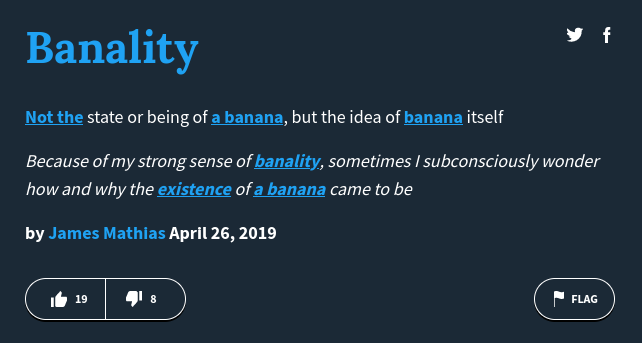
\includegraphics[width=0.7\textwidth]{Screenshot from 2023-03-09 14-36-16.png}
\end{figure}

\newpage
\section{\textcolor{red}{Lezione 7 \space\space 13/03/'23}}
\paragraph{\textcolor{red}{Esempio}}
Stabilire per quali valori del parametro $\alpha>0$ converge la serie
\begin{empheq}{equation*}
    \sum_{n=1}^{\infty} (n-\cos{n^\alpha})\left(\frac{1}{n}-\sin{\frac{1}{n^{2\alpha}}}\right)
\end{empheq}
\begin{empheq}{equation*}
    n-\cos{n^\alpha} \sim n \,\,\,\,\, \text{per} \,\,\,\,\, n \rightarrow +\infty
\end{empheq}
\begin{empheq}{align*}
    \sin y &= y- \frac{1}{6}y^3+o(y^4) \,\,\,\,\, \text{ per} \,\,\,\,\, y \rightarrow 0\\
    \sin \frac{1}{n^{2\alpha}} &=\frac{1}{n^{2\alpha}}-\frac{1}{6}\frac{1}{n^{6\alpha}} +o\left(\frac{1}{n^{8\alpha}}\right)
\end{empheq}
\begin{empheq}{align*}
    (n-\cos{n^\alpha})\left(\frac{1}{n}-\sin{\frac{1}{n^{2\alpha}}}\right) &=(n+o(n))\left[\frac{1}{n}-\frac{1}{n^{2\alpha}}+\frac{1}{6}\frac{1}{n^{6\alpha}}+o\left(\frac{1}{n^{8\alpha}}\right)\right]\\
    &=1-\frac{1}{n^{2\alpha-1}}+\frac{1}{6}\frac{1}{n^{6\alpha-1}}+o(1)
\end{empheq}
Se $2\alpha-1 \neq 0 \Longrightarrow \lim_{n\rightarrow +\infty} 1-\frac{1}{n^{2\alpha-1}}+\frac{1}{6}\frac{1}{n^{6\alpha-1}}+o(1)   \neq 0$ perchè, se $2\alpha-1>0$, $\frac{1}{n^{2\alpha - 1}}+\frac{1}{6}\frac{1}{n^{6\alpha-1}}+o(1) \rightarrow 0$ e quindi il limite fa 1, mentre se $2\alpha-1 < 0$, il limite è $-\infty \Longrightarrow $ se $2\alpha-1\neq 0$, la serie non converge (diverge).\\
Concentriamoci sul caso $\alpha=\frac{1}{2}$, cioè $2\alpha-1=0$. Il termine generale della mia serie è
\begin{empheq}{align*}
    (n-\cos{\sqrt{n}})\left(\frac{1}{n} - \sin{\frac{1}{n}}\right) &= (n-\cos{\sqrt{n}})\left( \frac{1}{n}-\frac{1}{n} +\frac{1}{6} \frac{1}{n^3}+ o\left( \frac{1}{n^4}\right) \right)= \\
    &=\frac{1}{6}\frac{1}{n^2}-\frac{1}{6}\frac{\cos{\sqrt{n}}}{n^2}+o(\frac{\cos{\sqrt{n}}}{n^n})=\\
    &=\frac{1}{6} \frac{1}{n^2}-\frac{1}{6}\frac{\cos{\sqrt{n}}}{n^3} + o\left( \frac{\cos{\sqrt{n}}}{n^n} \right)=\\
    &= \frac{1}{6} \frac{1}{n^2} +o\left( \frac{1}{n^2} \right) \sim \frac{1}{n^2}
\end{empheq}
che essendo $>0$ definitivamente per $n\rightarrow + \infty$ ci permette di dire che $\sum_{n=1}^{\infty} \frac{1}{n^2}$ converge, per il criterio asintotico del confronto anche la serie di partenza converge.\\
\textcolor{orange}{A posteriori, il termine generale è $(n+\cos{\sqrt{n}})(\frac{1}{n}-\sin{\frac{1}{n}})= (n+o(n))(\frac{1}{6}\frac{1}{n^3}+o(\frac{1}{n^4})) =\frac{1}{6}\frac{1}{n^2}+o(\frac{1}{n^2})$}

\subsection{\textcolor{red}{Integrali impropri}}
\paragraph{\textcolor{red}{Ripasso: Integrali secondo Riemann}}

Data $f:[a,b]\rightarrow\R$ limitata si ha $a=x_0 < x_1 < ... < x_n =b$ si hanno
\begin{empheq}{align*}
    S(f)&=\sum_{i=1}^{n} \left(\sup_{[x_{i-1},x_i]} f(x)\right)\cdot (x_i-x_{i-1}) \,\,\,\,\, \text{somma superiore,}\\
    s(f)&=\sum_{i=1}^{n} \left(\inf_{[x_{i-1},x_i]} f(x)\right)\cdot (x_i-x_{i-1}) \,\,\,\,\, \text{somma inferiore.}
\end{empheq}
Se $\inf_{a=x_0 < x_1 < ... < x_n =b} S(f) = \sup_{a=x_0 < x_1 < ... < x_n =b} s(f) =I \in \R$ allora $f$ si dice Riemann integrabile in $[a,b]$ e si pone 
\begin{empheq}{equation*}
    \int_{a}^{b} f(x)dx=I.
\end{empheq}

\paragraph{\textcolor{red}{Esempio}}

\begin{equation*}
    f(x)=\frac{1}{x^\alpha}, \,\,\,\,\,\, x \geq 1, \,\,\,\, \alpha \in \R
\end{equation*}
Vogliamo definire, se possibile, 
\begin{equation*}
    \int_{1}^{+\infty} f(x) dx= \int_{1}^{+\infty}\frac{1}{x^\alpha}dx
\end{equation*}
Stiamo provando ad integrare una funzione limitata su un intervallo illimitato.\\
\begin{figure}[h!]
    \centering
    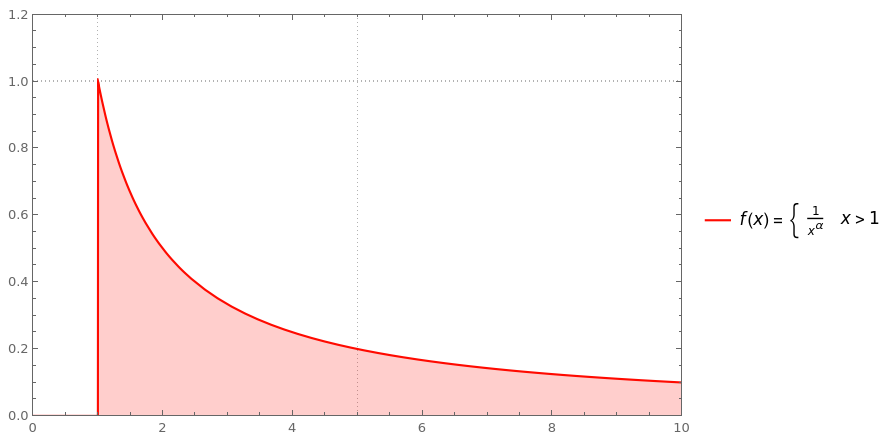
\includegraphics[width=\textwidth]{unosuxallaalpha.png}
\end{figure}

Fissato $c > 1$, riesco a definire $\int_{1}^{c} f(x)dx$ perchè integro una funzione limitata su un intervallo limitato.\\
Posso dunque definire
\begin{empheq}{align*}
    \int_{1}^{+\infty} f(x)dx &=\lim_{c\rightarrow +\infty} \int_{1}^{c}f(x)dx, \,\,\,\,\, \text{se}\,\,\, \exists\\
    \int_{1}^{+\infty} \frac{1}{x^\alpha} dx &= \lim_{c \rightarrow + \infty}\int_{1}^{c} \frac{1}{x^\alpha}dx\\
    &=
    \begin{cases}
        & \lim_{c \rightarrow +\infty}\frac{1}{1-\alpha}[c^{1-\alpha}-1]\,\,\,\, \text{se}\,\,\, \alpha \neq 1\\
        & \lim_{c \rightarrow +\infty} \ln c \,\,\,\, \text{se} \,\,\, \alpha=1
    \end{cases}\\
    &=
    \begin{cases}
        & \frac{1}{\alpha-1} \,\,\,\, \text{se} \,\,\, \alpha > 1\\
        &+\infty \,\,\,\, \text{se} \,\,\, \alpha \leq 1
    \end{cases}
\end{empheq}

\paragraph{\textcolor{red}{Esempio}}
\begin{empheq}{equation*}
    f(x)=-\ln x, \,\,\, x \in ]0,1]
\end{empheq}
e provo a definire 
\begin{empheq}{equation*}
    \int_{0}^{1} f(x)dx
\end{empheq}
cioè l'integrale di una funzione illimitata su un intervallo limitato.\\

\begin{figure}[h!]
    \centering
    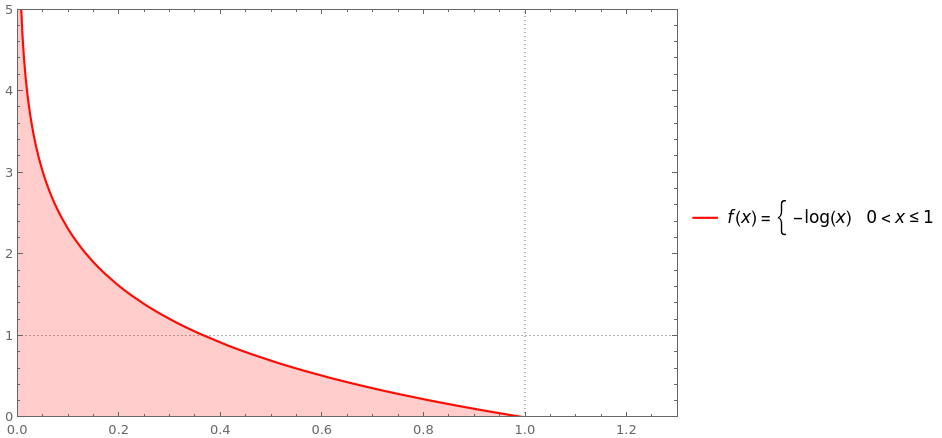
\includegraphics[width=\textwidth]{intda1a0.png}
\end{figure}
Riesco a definire bene $\int_{c}^{1} f(x)dx$ perchè integro una funzione limitata
\textcolor{orange}{$(|f(x)|\leq -\ln c \forall x\in[c,1])$} su un intervallo limitato.\\
Posso dunque definire
\begin{empheq}{align*}
    \int_{0}^{1} f(x)dx &= \lim_{c\rightarrow +0^+} \int_{c}^{1} f(x)dx\,\,\,\,\,\, \text{se}\,\,\, \exists\\
    \int_{0}^{1}(-\ln x) dx &= \lim_{c \rightarrow 0^+} \int_{c}^{1}(-\ln x)dx\\
    &= \lim_{c \rightarrow 0^+} [x-x\ln x]_{c}^{1} \\
    &= \lim_{c \rightarrow 0^+} [1-c+c\ln c]=1
\end{empheq}

\paragraph{\textcolor{red}{Definizione}}
Sia $f:[a,b[\rightarrow \R, a,b \in \R \cup\{+\infty\}$ \textcolor{orange}{(voglio definire $\int_{a}^{b}f(x)dx$)} Riemann integrabile in $[a,c]\,\, \forall c \in [a,b[$. Se $\exists$ finito il $\lim_{c \rightarrow b^-} \int_{a}^{c}f(x)dx $, allora $f$ si dice integrale in senso improprio o generalizzato in $[a,b[$ e la quantità 
\begin{empheq}{equation*}
    \int_{a}^{b} f(x)dx = \lim_{c\rightarrow b^-} \int_{a}^{c} f(x)dx
\end{empheq}
si dice integrale improprio o generalizzato di $f$ in $[a,b[$.\\
Analogamente, data $f:]a,b]\rightarrow \R, a,b \in \R \cup \{-\infty\}$, Riemann integrabile in $[c,b]\,\, \forall c \in ]a,b]$. Se $\exists$ finito il $\lim_{c \rightarrow a^+} \int_{c}^{b} f(x)dx$, allora $f$ si dice integrabile in senso improprio o generalizzato in $]a,b]$ e la quantità
\begin{empheq}{equation*}
    \int_{a}^{b} f(x)dx = \lim_{c \rightarrow a^+} \int_{c}^{b} f(x)dx
\end{empheq}
si dice integrale improprio o generealizzato di $f$ in $]a,b]$.\\
Se $f$ è integrabile in senso improprio in un intervallo $I$, allora si dice anche che l'integrale (improprio) di $f$ in $I$ è convergente o che $f$ ha integrale (improprio) convergente in $I$.\\
Se il limite che definisce l'integrale improprio di $f$ è infinito, si dice anche che l'integrale (improprio) di $f$ è divergente o che $f$ ha integrale (improprio) divergente in $I$.

\paragraph{\textcolor{red}{Osservazione}}
Vista la definizione, 
\begin{empheq}{equation*}
    \int_{1}^{+\infty}\frac{1}{x^\alpha}dx \,\,\,\,\, \text{converge} \Leftrightarrow \alpha > 1
\end{empheq}

\paragraph{\textcolor{red}{Esempio Importante}}
\begin{empheq}{equation*}
    f(x)=\frac{1}{(x-a)^\alpha}, \,\,\,\, x \in ]a,a+1], \,\,\, a\in \R \,\, \text{fissato},\,\,\, \alpha\in\R\,\,\, \text{parametro},\,\,\, \alpha > 0
\end{empheq}
Studiamo la convergenza di 
\begin{empheq}{align*}
    \int_{a}^{a+1} \frac{1}{(x-a)^\alpha} dx  &= \lim_{c \rightarrow a^+} \int_{c}^{a+1} \frac{1}{(x-a)^\alpha} dx\\
    &=
    \begin{cases}
        & \lim_{c \rightarrow a^+} \frac{1}{1-\alpha}[1-(c-a)^{1-\alpha}] \,\,\,\, \text{se}\,\, \alpha \neq 1 \\
        & \lim_{c \rightarrow a^+} -\ln(c-a)\,\,\,\, \text{se} \,\, \alpha =1
    \end{cases}\\
    &=
    \begin{cases}
        & \frac{1}{1-\alpha} \,\,\,\, \text{se}\,\, \alpha <1 \\
        &+\infty \,\,\,\, \text{se}\,\, \alpha \geq1.
    \end{cases}
\end{empheq}
Dunque 
\begin{empheq}{equation*}
    \int_{a}^{a+1} \frac{1}{(x-a)^\alpha} dx \,\,\,\, \text{converge} \Leftrightarrow \alpha < 1.
\end{empheq}
In particolare
\begin{empheq}{equation*}
    \int_{0}^{1} \frac{1}{x^\alpha} \,\,\,\, \text{converge} \Leftrightarrow \alpha < 1.
\end{empheq}

\paragraph{\textcolor{red}{Esempio}}
Stabilire se converge 
\begin{empheq}{equation*}
    \int_{0}^{1} \frac{\sin{\frac{1}{x}}}{x^2} dx
\end{empheq}
\begin{figure}[h!]
    \centering
    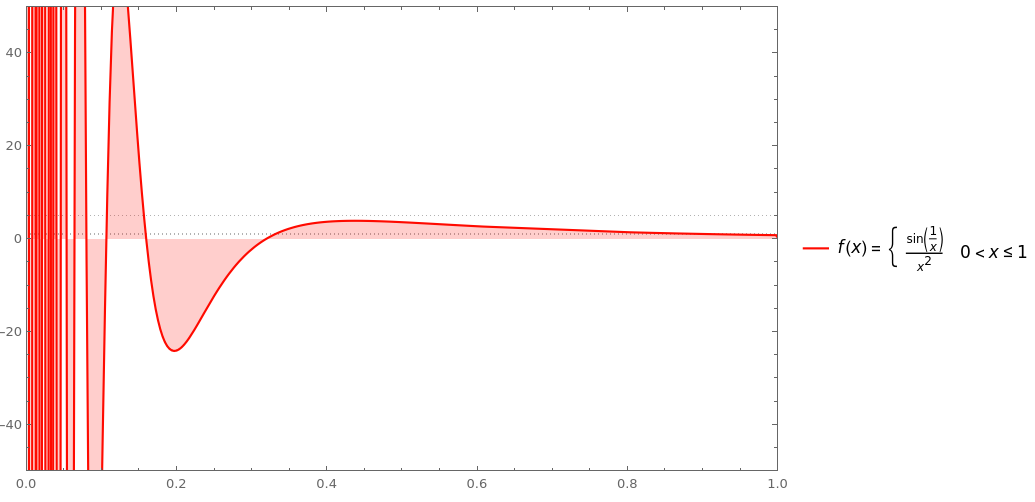
\includegraphics[width=\textwidth]{senobuffo.png}
\end{figure}

Devo calcolare 
\begin{empheq}{equation*}
    \lim_{c\rightarrow0^+} \int_{c}^{1} \frac{\sin{\frac{1}{x}}}{x^2} dx= \lim_{c \rightarrow 0^+} \cos{\frac{1}{x}}|_{c}^{1}=\lim_{c\rightarrow 0^+}\left(1-\cos{\frac{1}{c}}\right)
\end{empheq}
che non esiste $\Rightarrow$ la funzione $f(x)=\frac{\sin{\frac{1}{x}}}{x^2}$, non è integrabile in senso improprio in $]0,1]$.

\paragraph{\textcolor{red}{Esempio Importante}}
\begin{empheq}{align*}
    \int_{0}^{+\infty} e^{\alpha x} dx &=\lim_{c \rightarrow +\infty} \int_{0}^{c} e^{\alpha x} dx \\&= \lim_{c \rightarrow +\infty} \frac{1}{\alpha}(e^{\alpha c}-1)\\
    &= \begin{cases}
        & -\frac{1}{\alpha} \,\,\,\, \text{se} \,\, \alpha <0\\
        &+\infty \,\,\,\, \text{se} \,\, \alpha >0.
    \end{cases}
\end{empheq}
\begin{empheq}{equation*}
    \int_{0}^{+\infty} e^{\alpha x} \,\,\,\,\, \text{converge} \Leftrightarrow \,\,\, \alpha <0.
\end{empheq}
Analogamente
\begin{empheq}{equation*}
    \int_{-\infty}^{0} e^{\alpha x} dx \,\,\,\,\, \text{converge} \Leftrightarrow \,\,\, \alpha > 0.
\end{empheq}
Dato $ a>0$, scrivendo $e^{\alpha x} = e^{(\alpha \ln a)x}$ si deduce la convergenza degli integrali
\begin{empheq}{align*}
    &\int_{-\infty}^{0} e^{\alpha x} dx \\
    &\int_{0}^{+\infty}  e^{\alpha x} dx.
\end{empheq}
\text{\textcolor{orange}{(Facile esercizio per casa)}}

\paragraph{\textcolor{red}{Nota Bene}}
$f:[1,+\infty[ \rightarrow \R$ continua. E' vero o falso che $\lim_{x \rightarrow +\infty} f(x)=0 \Rightarrow \int_{1}^{+\infty} f(x)dx$ converge?\\
E' falso!!! Si veda $f(x)=\frac{1}{x}$\\
E' vero o falso che
$\int_{1}^{+\infty}f(x) dx$ converge $\Rightarrow \lim_{x \rightarrow +\infty} f(x)=0$?\\
E' falso!!!\\
\begin{figure}[h!]
    \centering
    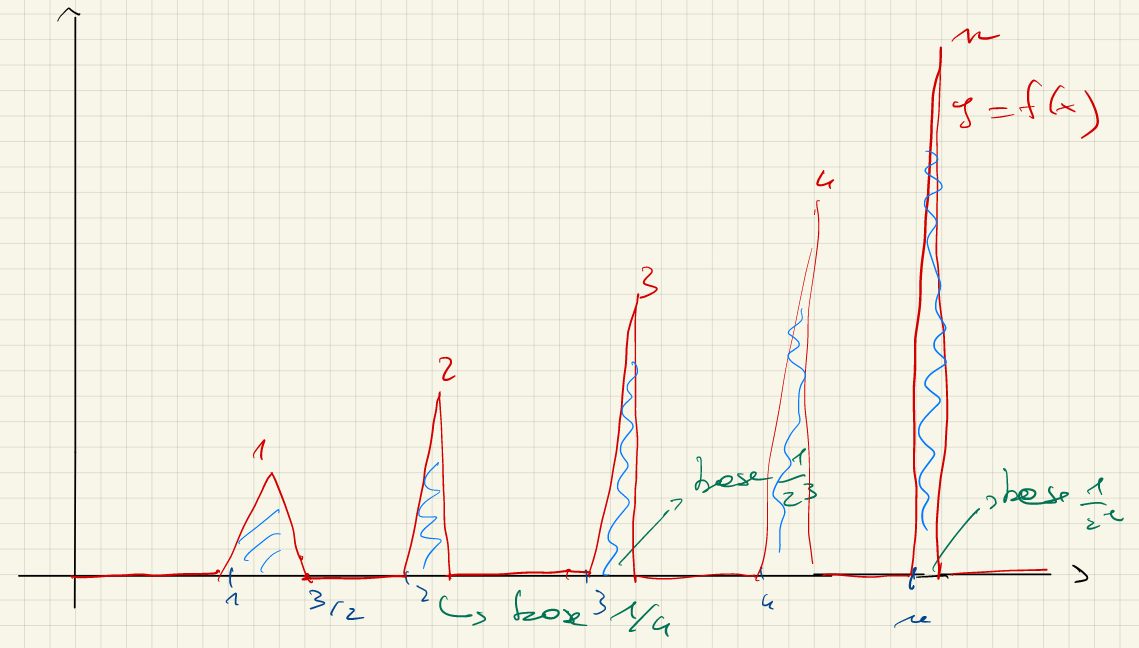
\includegraphics[width=\textwidth]{cosiappuntiti.png}
\end{figure}

Ad ogni numero naturale $n$ costruite un triangolo di base $\frac{1}{2^n}$ e altezza $n$

\begin{empheq}{equation*}
    \int_{1}^{+\infty} f(x)dx = \sum (\text{aree dei triangoli}) = \sum_{n=1}^{\infty} \frac{1}{2} \frac{1}{2^n} \cdot n = \frac{1}{2} \sum_{n=1}^{\infty} \frac{n}{2^n}, 
\end{empheq}
che è una serie convergente.

\paragraph{\textcolor{red}{Osservazione}}
Se $f:[a,b] \rightarrow \R$ è Riemann integrabile, allora è integrabile anche in senso improprio e i due integrali coincidono.

\paragraph{\textcolor{red}{Definizione}}
$f:[a,b] \rightarrow \R,\,\, a,b \in \R \cup \{\pm \infty\}$, Riemann integrabile in $[c,d]\,\, \forall a<c<d<b$. $f$ si dice integrabile in senso improprio in $ ]a,b[$ se, fissato $\xi \in ]a,b[$, lo è in $]a, \xi]$ e in $[\xi,b[$ \textcolor{orange}{(esistono finiti $\lim_{c \rightarrow a^+} \int_{c}^{\xi} f(x)dx$ e $\lim_{d\rightarrow b^-}\int_{\xi}^{d} f(x)dx$)} e in tal caso si pone 
\begin{empheq}{equation*}
    \int_{a}^{b} f(x)dx = \int_{a}^{\xi} f(x)dx + \int_{\xi}^{b} f(x) dx
\end{empheq}
Si verifica che la definizione non dipende da punto $\xi$ fissato.


\paragraph{\textcolor{red}{Esempio}}
Come si integra $\int_{-\infty}^{+\infty} \frac{1}{1+x^2}dx$?\\
$x \mapsto \frac{1}{1+x^2}$ è integrabile secondo Riemann in $[c,d] \,\, \forall c<d$. \\
Sia $\xi = 2$. Dobbiamo verificare se la funzione è integrabile in senso improprio in $]-\infty,2] $ e in $ [2, +\infty[$
\begin{empheq}{align*}
    &\int_{-\infty}^{2}\frac{1}{1-x^2}dx = \lim_{c \rightarrow -\infty} \int_{c}^{2} \frac{1}{1+x^2}dx = \lim_{c \rightarrow -\infty} \left(\arctan{2+\frac{\pi}{2}}\right)= \arctan{2+\frac{\pi}{2}}\\
    &\int_{2}^{+\infty}\frac{1}{1-x^2} dx =\lim_{c \rightarrow +\infty} \int_{2}^{c} \frac{1}{1-x^2}dx=\lim_{c \rightarrow +\infty} (\arctan{c}-\arctan{2})=\frac{\pi}{2}-\arctan{2}\\
&\Rightarrow \int_{-\infty}^{+\infty} \frac{1}{1+x^2}dx \,\,\,\, \text{converge e}\,\,\, \int_{-\infty}^{+\infty}\frac{1}{1+x^2}dx = \int_{-\infty}^{2}\frac{1}{1+x^2} dx+ \int_{2}^{+\infty}\frac{1}{1+x^2}dx
\end{empheq}

\paragraph{\textcolor{red}{Esempio}}
\begin{empheq}{align*}
    &f(x)=\frac{1}{x^\alpha}, \,\,\,\,\,x \in ]0,+\infty[\\
    &\alpha > 0 \Rightarrow \lim_{x \rightarrow 0^+} f(x)=+\infty.
\end{empheq}
Preso $\xi=1$, $f$ è integrabile in senso improprio in $]0,+\infty[ \Leftrightarrow$ entrambi gli integrali $\int_{0}^{1} \frac{1}{x^\alpha} dx$ e $\int_{1}^{+\infty} \frac{1}{x^\alpha} dx$ convergono ma
\begin{empheq}{align*}
    &\int_{0}^{1}\frac{1}{x^\alpha}dx \,\,\,\,\, \text{converge} \Leftrightarrow \alpha <1 \\
   & \int_{1}^{+\infty} \frac{1}{x^\alpha}dx \,\,\,\,\, \text{converge} \Leftrightarrow \alpha > 1\\
   & \Rightarrow \int_{0}^{+\infty} \frac{1}{x^\alpha}dx \,\,\,\text{non converge per alcun valore di} \,\, \alpha
\end{empheq}

\paragraph{\textcolor{red}{Esempio}}
\begin{empheq}{equation*}
    f(x)= 
    \begin{cases}
        & e^x\,\,\,\,\, \text{se} x \leq 1 \\
        & \frac{1}{x \sqrt{x-1}}\,\,\,\,\, \text{se}\,\,\, x>1
    \end{cases}
\end{empheq}
vogliamo stabilire se $\int_{-\infty}^{+\infty}f(x)dx$ converge.\\
\begin{figure}[h!]
    \centering
    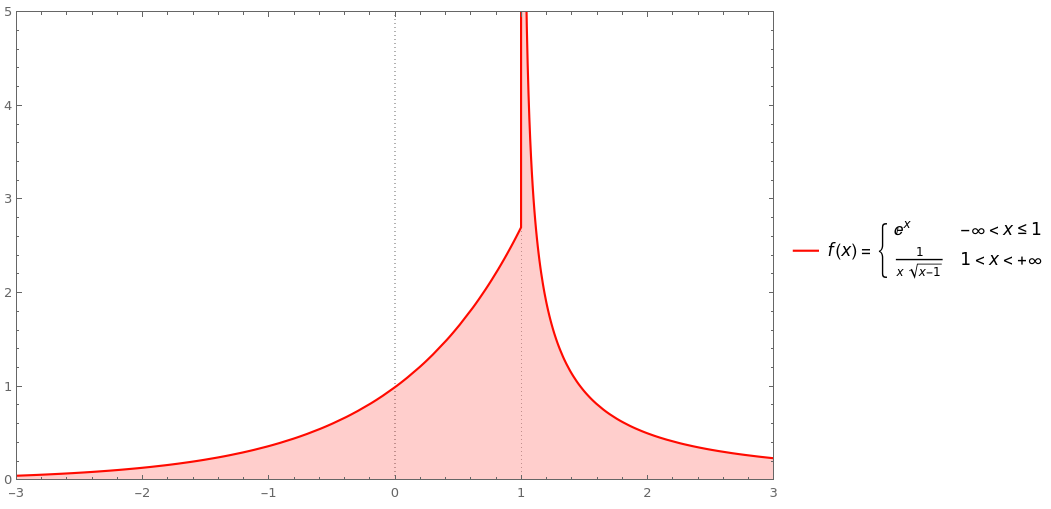
\includegraphics[width=\textwidth]{espefrac.png}
\end{figure}

Devo studiare $\int_{-\infty}^{1}f(x) dx = \int_{-\infty}^{1}e^x dx$ e, prendendo $\xi=3$,  $\int_{1}^{3}f(x)dx$ e $\int_{3}^{+\infty}f(x)dx$. Se tutti convergono, anche $\int_{-\infty}^{+\infty} f(x)dx$ converge e 
\begin{empheq}{equation*}
    \int_{-\infty}^{+\infty} f(x)dx = \int_{-\infty}^{1} f(x)dx + \int_{1}^{3} f(x)dx + \int_{3}^{+\infty} f(x)dx
\end{empheq}

\paragraph{\textcolor{red}{Ulteriore Definizione}}
In generale, data $f:]a,b[\rightarrow \R$ integrabile in senso improprio in $]x_0,x_1[,]x_1,x_2[,...,]x_{n-1},x_n[$ con $a= x_0 <x_1<...<x_n=b$, allora $f$ si dice integrabile in senso improprio in $]a,b[$ e si pone 
\begin{empheq}{equation*}
    \int_{a}^{b}f(x)dx= \sum_{i=1}^{n} \int_{x_{i-1}}^{x_i}f(x)dx.
\end{empheq}

\newpage
\section{\textcolor{red}{Lezione 8\space\space 14/03/'23}}
\subsection{\textcolor{red}{Criteri di integrabilità}}
\paragraph{\textcolor{red}{Proposizione}}
Sia $f:[a,b[\rightarrow \R,\,\,\, b\in\R\cup \{+\infty\}$ tale che $f(x)\geq0$ definitivamente per $x \rightarrow b^-$ e tale che sia Riemann integrabile in $[a,b]\,\, \forall c\in [a,b[$. Allora esiste
\begin{equation*}
    \lim_{c \rightarrow b^-} \int_{a}^{c} f(x)dx
\end{equation*}
cioè l'integrale improprio $\int_{a}^{b} f(x)dx$ è ben definito \textcolor{orange}{(converge o diverge a $+\infty$)}.

\paragraph{\textcolor{red}{Dimostrazione}}
Per semplicità assumiamo $f(x)\geq 0 \,\,\, \forall\,\, x\in[a,b[$. Sia allora $F(x)=\int_{a}^{c} f(x)dx,\,\,\,c\in [a,b[$. Allora $F$ è monotona crescente, dunque, presi $c_2 > c_1$ si ha
\begin{equation*}
    F(c_2)-F(c_1)=\int_{a}^{c_2}f(x)dx - \int_{a}^{c_1} f(x)dx = \int_{c_1}^{c_2} f(x)dx \geq 0
\end{equation*}
perchè $f(x)\geq 0 \,\,\forall x \in [c_1,c_2] \Rightarrow F(c_2)\geq F_{c_1}$.\\
$F$ ha limite per $c \rightarrow b^-$, cioè esiste
\begin{equation*}
    \lim_{c \rightarrow b^-} F(c)=\lim_{c \rightarrow b^-} \int_{a}^{b} f(x)dx.
\end{equation*}
Un risultato analogo si enuncia per funzioni definitivamente $\leq 0$ per $ x\rightarrow b^-$ o per una funzione $f:]a,b]\rightarrow \R,\,\,\, a\in\R\cup\{-\infty\}$.
\begin{flushright}
\large\Lightning
\end{flushright}

\paragraph{}
Come per le serie ci concentriamo su criteri di integrabilità per funzioni di segno definito.

\subsubsection{\textcolor{red}{Teorema: Criterio del confronto}}
\paragraph{\textcolor{red}{Teorema}}
$f,g:[a,b[\rightarrow\R, \,\, b\in\R\cup\{+\infty\}$, Riemann integrabili in $[a,c] \,\, \forall c \in [a,b[$ e tali che $0\leq f(x) \leq g(x)$ definitivamente per $x \rightarrow b^-$.
\begin{enumerate}
    \item Se $\int_{a}^{b}g(x)dx$ converge, allora converge anche $\int_{a}^{b} f(x)dx$.
    \item Se $\int_{a}^{b} f(x)dx$ diverge, allora diverge anche $\int_{a}^{b}g(x)dx$.
\end{enumerate}
Un risultato analogo vale per funzioni $f,g:]a,b]\rightarrow\R, \,\, a\in\R\cup\{-\infty\}$, con ovvie modifiche.

\paragraph{\textcolor{red}{Dimostrazione}}
Per semplicità assumiamo $0 \leq f(x)\leq g(x) \,\,\, \forall x \in [a,b[$.
\begin{enumerate}
    \item $\exists$ finito $\lim_{c \rightarrow b^-} \int_{a}^{c} g(x) dx \,\, \forall c \in [a,b[,\,\,\, \int_{a}^{c}f(x)dx \leq \int_{a}^{c} g(x)dx$ perchè $f(x)\leq g(x)$. Allora $\lim_{c \rightarrow b^-} \int_{a}^{c} f(x)dx \leq \lim_{c \rightarrow b^-} \int_{a}^{c} g(x)dx$ \textcolor{orange}{(che esistono perchè $f(x)\geq 0$)} e quindi $\lim_{c \rightarrow b^-} \int_{a}^{c} f(x)dx $ esiste finito e $\int_{a}^{b} f(x)dx$ è convergente.
    \item $\lim_{c \rightarrow b^-} \int_{a}^{c} f(x) dx = +\infty $ \textcolor{orange}{($f(x)\geq 0$)}, allora $\int_{a}^{c} g(x)dx \geq \int_{a}^{c} f(x) dx \,\,\, \forall c \in [a,b[$ $\Rightarrow \lim_{c \rightarrow b^-} \int_{a}^{c} g(x)dx =+\infty$ per il teorema del confronto sui limiti.
\end{enumerate}
\begin{flushright}
\large\Lightning
\end{flushright}

\subsubsection{\textcolor{red}{Teorema: Criterio di assoluta integrabilità}}
\paragraph{\textcolor{red}{Teorema}}
$f:[a,b[\rightarrow \R, b \in \R \cup \{+\infty\}$ Riemann integrabile in $[a,c] \,\,\, \forall c \in [a,b[$ e tale che $|f|$ è integrabile in senso improprio in $[a,b[$ \textcolor{red}{(si dice che l'integrale improprio di $f$ è assolutamente convergente o che converge assolutamente)}. Allora $\int_{a}^{b} f(x)dx$ converge.

\paragraph{\textcolor{red}{Dimostrazione}}
$f=f^+-f^-$ ove $f^+=\max\{f(x),0\} \geq 0$ e $f^-=\min\{f(x),0\} \geq 0$ $\forall x \Rightarrow |f(x)|=f^+(x)+f^-(x)$\\
\begin{figure}[h!]
    \centering
    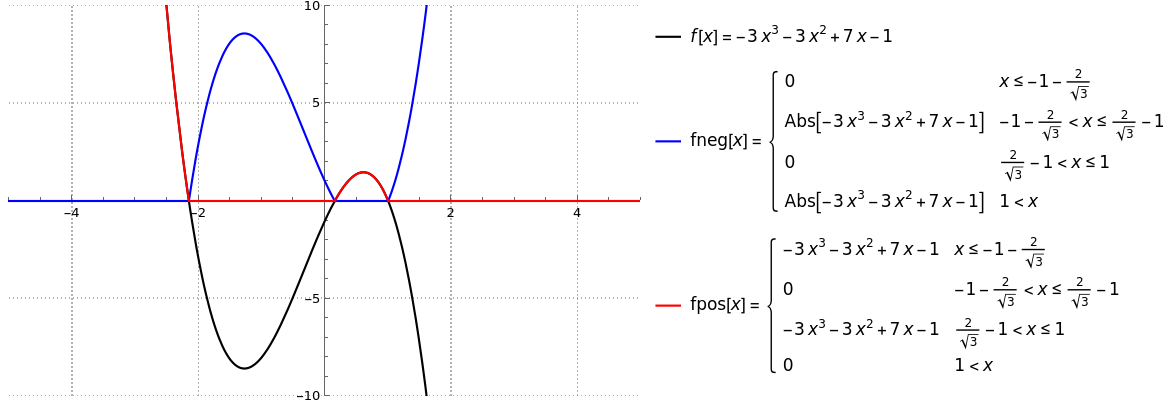
\includegraphics[width=\textwidth]{fposfneg.png}
\end{figure}

$f^+$ e $f^-$ sono Riemann integrabili  in  $[a,c]\,\,\, \forall c\in [a,b[$ e inoltre
\begin{equation*}
\begin{cases}
    & 0 \leq f^+(x) \leq |f(x)|\\
    & 0 \leq f^-(x) \leq |f(x)|
\end{cases}
 \,\,\,\,\, \forall x \in [a,b[
\end{equation*}
$\Longrightarrow$ per il criterio del confronto $\int_{a}^{b} f^+(x)dx$ e $\int_{a}^{b} f^-(x)dx$ convergono entrambi $\Rightarrow \lim_{c \rightarrow b^-} \int_{a}^{c} f(x)dx = \lim_{c \rightarrow b^-} \left[ \int_{a}^{c}f^+(x)dx - \int_{a}^{c}f^-(x)dx \right]$, esiste finito per il teorema sulla somma dei limiti $\Rightarrow \int_{a}^{b} f(x) dx$ converge.

\paragraph{\textcolor{red}{Osservazione}}
Sia $f: [a,b[ \rightarrow \R, \,\, b\in\R\cup\{+\infty\}$ e se $\int_{a}^{b} f(x) dx$ converge, non è detto che $\int_{a}^{b}|f(x)|dx$ converga.
Prendiamo
\begin{equation*}
    f(x)= \frac{\sin x}{x}, \,\,\,\,\, x \geq 1
\end{equation*}
e dimostriamo che $ \int_{1}^{+\infty} \frac{\sin x}{x} dx$ converge. Fissiamo $c>1$
\begin{equation*}
    \int_{1}^{c} \frac{\sin x}{x} dx= -\frac{\cos x}{x} |_{1}^{c} - \int_{1}^{c} \frac{\cos x}{x^2} dx = \cos 1 - \frac{\cos c}{c} -\int_{1}^{c} \frac{\cos x}{x^2} dx
\end{equation*}
\begin{equation*}
    \lim_{c \rightarrow +\infty} \int_{1}^{c} \frac{\sin x}{x} dx =\lim_{c \rightarrow +\infty} \left[\cos 1 -\frac{\cos c}{c} - \int_{1}^{c} \frac{cosx}{x^2}dx\right] 
\end{equation*}
\textcolor{orange}{($\lim_{c \rightarrow +\infty} \int_{1}^{c} \frac{\cos x}{x^2} dx$ esiste finito)}\\
$\frac{|\cos x|}{x^2} \leq \frac{1}{x^2} \,\,\, \forall x \geq 1$ e $ \int_{1}^{+\infty} \frac{1}{x^2} dx$ converge $\Rightarrow \int_{1}^{+\infty} \frac{|\cos x|}{x^2} dx$ converge per il criterio del confronto $\Rightarrow \int_{1}^{+\infty} \frac{\cos x}{x^2}dx$ converge per il criterio di assoluta integrabilità\\
$\Rightarrow \lim_{c \rightarrow +\infty} \int_{1}^{c} \frac{\sin x}{x} dx = \cos 1 - \int_{1}^{+\infty} \frac{\cos x}{x^2} dx$ esiste finito e dunque $\int_{1}^{+\infty} \frac{\sin x}{x} dx$ converge ma $\int_{1}^{+\infty} |\frac{\sin x}{x}|dx =+\infty$.\\
Presi $k \geq 1, \,\,\, k \in \N$ avremo $k\pi \leq x \leq (k+1)\pi \Longrightarrow \frac{1}{(k+1)\pi} \leq \frac{1}{x} \leq \frac{1}{k\pi} \Longrightarrow \int_{k\pi}^{(k+1)\pi} \frac{(\sin x)}{x}dx \geq \int_{k\pi}^{(k+1)\pi} \frac{1}{(k+1)\pi} (\sin x) dx = \frac{2}{(k+1)\pi} \Longrightarrow \int_{1}^{+\infty} \frac{|\sin{x}|}{x} dx \geq \sum_{k=1}^{\infty} \int_{k\pi}^{(k+1)\pi} \frac{|\sin{x}|}{x} dx \geq \sum_{k=1}^{\infty} \frac{2}{(k+1)\pi}=+\infty$  perchè $\frac{2}{(k+1)\pi} \sim \frac{1}{k}$.

\subsubsection{\textcolor{red}{Teorema: Criterio asintotico del confronto}}
\paragraph{\textcolor{red}{Teorema}}
$f,g: [a,b[\rightarrow \R, \,\,\ b\in \R \cup \{+\infty\}$, Riemann integrabili in $[a,c] \,\, \forall c \in [a,b[$ tali che $f(x),g(x)\geq 0$ definitivamente per $x \rightarrow b^-$ e $\lim_{x \rightarrow b^-} \frac{f(x)}{g(x)}=l \in [0,+\infty[$
\begin{enumerate}
    \item Se $l \in \,\, ]0,+\infty[$, allora $ \int_{a}^{b} f(x) dx$ converge $\Leftrightarrow \int_{a}^{b} g(x) dx$ converge.
    \item Se $l=0$ e $\int_{a}^{}b g(x)dx $ converge, allora $\int_{a}^{b} f(x) dx$ converge.
    \item Se $l=+\infty$ e $\int_{a}^{b} g(x) dx$ diverge, allora $\int_{a}^{b} f(x)dx$ diverge.
\end{enumerate}

\paragraph{\textcolor{red}{Dimostrazione}}
\begin{enumerate}
    \item $\lim_{x \rightarrow b^-}\frac{f(x)}{g(x)} = l \in \,\, ]0,+\infty[$ allora $\frac{l}{2}\leq \frac{f(x)}{g(x)}\leq 2l$ definitivamente per $x \rightarrow b^-$ perchè $]\frac{l}{2},2l[$ è un intorno di $l$. Dunque $f(x)\leq 2lg(x)$ e $g(x)\leq \frac{2}{l} f(x)$ definitivamente per $x \rightarrow b^-$. Se $\int_{a}^{b} g(x) dx$ converge $\int_{a}^{b} f(x) dx$ converge e se $\int_{a}^{b} f(x) dx$ converge $\int_{a}^{b} (x) dx$ per il criterio del confronto.
    \item $\lim_{x \rightarrow b^-} \frac{f(x)}{g(x)} = 0 \Rightarrow \frac{f(x)}{g(x)} \leq 1 $ definitivamente per $x\rightarrow b^- \Rightarrow f(x) \leq g(x)$ definitivamente per $x\rightarrow b^- \Rightarrow $ se $\int_{a}^{b} g(x)dx$ converge, allora $\int_{a}^{b} f(x)dx$ converge per il criterio del confronto.
    \item $\lim_{x \rightarrow b^-}\frac{f(x)}{g(x)} = +\infty \Rightarrow \frac{f(x)}{g(x)} \geq 1$ definitivamente per $x \rightarrow b^- \Rightarrow f(x) \geq g(x)$ definitivamente per $x \rightarrow b^- \Rightarrow$ se $\int_{a}^{b} g(x)dx$ diverge, allora $\int_{a}^{b} f(x)dx$ diverge sempre per il criterio del confronto.
\end{enumerate}
\begin{flushright}
\large\Lightning
\end{flushright}

\paragraph{\textcolor{red}{Esempio importante}}
Studiamo la convergenza di 
\begin{equation*}
    \int_{2}^{+\infty} \frac{1}{x^\alpha(\ln x)^\beta}dx, \,\,\,\,\,\, \alpha,\beta \in \R
\end{equation*}
\begin{itemize}
    \item Se $\alpha >1 \Rightarrow \int_{2}^{+\infty}\frac{1}{x^\alpha}dx$ converge
    \begin{itemize}
        \item Se $\beta \geq 0 \Rightarrow \frac{1}{x^\alpha(\ln x)^\beta} \leq \frac{1}{x^\alpha}$ per $x>a \Rightarrow \int_{2}^{+\infty} \frac{1}{x^\alpha(\ln x)^\beta}dx$ converge
        \item Se $\beta <0 \Rightarrow \frac{1}{x^\alpha(\ln x)^\beta} = \frac{(\ln x)^{-\beta}}{x^\alpha}$.\\ Preso $\epsilon > 0$ si ha $\ln x \leq x^\epsilon$ definitivamente per $x \rightarrow+\infty$ $\Rightarrow \frac{(\ln x)^{-x}}{x^\alpha} \leq \frac{x^{-\epsilon \beta}}{x^\alpha}=\frac{1}{x^{\alpha+\epsilon\beta}}$ definitivamente per $x\rightarrow +\infty$.\\
        Scelgo $\epsilon$ in modo che $\alpha+\epsilon\beta > 1$, cioè $\epsilon < \frac{1-\alpha}{\beta}>0 \Rightarrow \int_{2}^{+\infty} \frac{1}{x^{\alpha+\epsilon\beta}}dx$ converge $\Rightarrow \int_{2}^{+\infty} \frac{1}{x^\alpha(\ln x)^\beta}dx$ converge.
    \end{itemize}
    \item Se $\alpha < 1 \Rightarrow \int_{2}^{+\infty} \frac{1}{x^\alpha}dx$ diverge
    \begin{itemize}
        \item Se $\beta \geq 0 \Rightarrow \frac{1}{x^\alpha(\ln x)^\beta }\geq$ \textcolor{orange}{?? integrale divergente} $\Rightarrow \frac{1}{x^\alpha(\ln x)^\beta}= \frac{(\ln x)^{-\beta}}{x^\alpha}$.\\
        Fissato $\epsilon>0, \,\,\ln x \leq x^\epsilon $ definitivamente per $x \rightarrow +\infty$ $\Rightarrow (\ln x)^{-\beta}\geq x^{-\epsilon\beta}$ defintivamente per $x \rightarrow +\infty$ $\Rightarrow \frac{1}{x^\alpha (\ln x)^\beta} \geq \frac{x^{-\epsilon\beta}}{x^\alpha} = \frac{1}{x^{\alpha+\epsilon\beta}}$ definitivamente per $x \rightarrow +\infty$.\\
        Scelgo  $\epsilon$ in modo che $ \alpha+\epsilon\beta < 1,\,\,\, \epsilon < \frac{1-\alpha}{\beta} $\\
        $\Rightarrow \int_{2}^{+\infty} \frac{1}{x^{\alpha+\epsilon\beta}}dx$ diverge $\Rightarrow \int_{2}^{+\infty} \frac{1}{x^\alpha(\ln x)^\beta}$ diverge per il criterio del confronto.
        \item  Se $\beta \leq 0 \Rightarrow \frac{1}{x^\alpha(\ln x)^\beta} = \frac{(\ln x)^{-\beta}}{x^\alpha} \geq \frac{1}{x^\alpha}$ e $\int_{2}^{+\infty}\frac{1}{x^\alpha}dx$ diverge $\Rightarrow \int_{2}^{+\infty} \frac{1}{x^\alpha (\ln x)^\beta}dx$ diverge per il criterio del confronto.
    \end{itemize}
    \item Se $\alpha=1 \Rightarrow \int_{2}^{+\infty} \frac{1}{x(\ln x)^\beta} dx$
    \begin{itemize}
        \item Se $\beta=0 \Rightarrow \int_{2}^{+\infty} \frac{1}{x}dx =+\infty$.
        \item Se $\beta \neq 0,1 \Rightarrow \int_{2}^{+\infty} \frac{1}{x(\ln x)^\beta}dx=\lim_{c \rightarrow +\infty} \int_{2}^{c}(\ln x)^{-\beta}\frac{1}{x} dx = \lim_{c \rightarrow +\infty} \frac{1}{1-\beta}(\ln x)^{1-\beta}|_{2}^{c}$ che è uguale a $\frac{(\ln 2)^{1-\beta}}{\beta -1}$ se $\beta >1$ e $+\infty$ se $\beta < 1$.
        \item Se $\beta = 1 \Rightarrow \int_{2}^{+\infty} \frac{1}{x \ln x}dx = \lim_{c \rightarrow +\infty}\int_{2}^{c} \frac{1}{x \ln x}dx = \lim_{c\rightarrow +\infty} \ln(\ln x)|_{2}^{c}=+\infty$.
    \end{itemize}
\end{itemize}
\begin{equation*}
    \textcolor{red}{
    \int_{2}^{+\infty} \frac{1}{x^\alpha(\ln x)^\beta}dx
    \,\,\,\, \text{converge} \,\,\,\,
    \Leftrightarrow \alpha > 1 \,\,\, \text{o} \,\,\, (\alpha=1 \,\,\, \text{e}\,\,\, \beta >1)}
\end{equation*}

\paragraph{\textcolor{red}{Esempio importante}}
Studiamo la convergenza 
\begin{empheq}{equation*}
    \int_{0}^{\frac{1}{2}}\frac{1}{x^\alpha|\ln x|^\beta}dx,\,\,\,\,\,\, \alpha,\beta \in \R
\end{empheq}
\begin{empheq}{align*}
    \int_{0}^{\frac{1}{2}} \frac{1}{x^\alpha|\ln x|^\beta}dx &= \lim_{c \rightarrow o^+} \int_{c}^{\frac{1}{2}} \frac{1}{x^\alpha|\ln x|^\beta}dx \\
    &= \lim_{c \rightarrow 0^+} \int_{2}^{\frac{1}{c}} \frac{1}{\frac{1}{t^\alpha}|\ln{\frac{1}{t}}|^\beta}\left(\frac{1}{t^2}\right)dt \\
    &= \lim_{c \rightarrow 0^+} \int_{2}^{\frac{1}{c}} \frac{1}{t^{2-\alpha}(\ln t)^\beta}dt \\
    &= \lim_{d \rightarrow +\infty} \int_{2}^{d} \frac{1}{t^{2-\alpha}(\ln 
    t)^\beta} dt =\int_{2}^{+\infty} \frac{1}{t^{2-\alpha}(\ln t)^\beta} dt
\end{empheq}
che converge $\Leftrightarrow 2-\alpha>1$ oppure ($2-\alpha = 1$ e $\beta>1$) $\Leftrightarrow \alpha <1$ oppure ($\alpha =1$ e $\beta>1$)\\
\begin{empheq}{equation*}
    \textcolor{red}{\int_{0}^{\frac{1}{2}}\frac{1}{x^\alpha|\ln x|^\beta}dx \,\,\,\, \text{converge} \,\,\,\,
    \Leftrightarrow \alpha < 1 \,\,\, \text{o} \,\,\, (\alpha=1 \,\,\, \text{e}\,\,\, \beta >1)}
\end{empheq}

\paragraph{\textcolor{red}{Esempio}}
Studiare la convergenza dell'integrale improprio
\begin{empheq}{equation*}
    \int_{-\infty}^{+\infty}e^{-x}dx \,\,\,(=\sqrt{\pi})
\end{empheq}
Devo studiare separatamente 
\begin{empheq}{equation*}
    \int_{-\infty}^{0} e^{-x^2}dx \,\,\,\,\,\, \text{e} \,\,\,\,\,  \int_{0}^{+\infty} e^{-x^2}dx 
\end{empheq}
e vedere se entrambi convergono. $x\mapsto e^{-x^2} $ è pari e dunque
\begin{empheq}{align*}
    \int_{-\infty}^{0} e^{-x^2} dx& = \lim_{c \rightarrow -\infty} \int_{c}^{0} e^{-x^2}dx\\
    &= \lim_{c \rightarrow -\infty} \int_{0}^{-c} e^{-t^2} dt \\
    &= \lim_{d\rightarrow +\infty} \int_{0}^{d} e^{-x^2}dx =\int_{0}^{+\infty} e^{-x^2} dx
\end{empheq}
\begin{empheq}{equation*}
    \int_{-\infty}^{0} e^{-x^2}dx \,\,\,\, \text{converge} \,\,\,\, \Leftrightarrow \int_{0}^{+\infty} e^{-x^2}dx \,\,\,\, \text{converge.}
\end{empheq}
$0 \leq e^{-x^2}\leq e^{-x} \,\,\,\, \forall x \geq 1$ e $\int_{0}^{+\infty}e^{-x}dx=1$, cioè converge $\Rightarrow$ per il criterio del confronto $\int_{0}^{+\infty} e^{-x^2}dx$ converge.

\paragraph{\textcolor{red}{Esempio}}
Studiare la convergenza dell'integrale improprio 
\begin{equation*}
    \int_{1}^{+\infty}\frac{x^\alpha e^{x^4}}{1+e^{4x^4}}dx
\end{equation*}
al variare di $\alpha \in \R$.\\
Per $x\rightarrow+\infty \Rightarrow \frac{x^\alpha e^{x^4}}{1+e^{4x^4}} \sim \frac{x^\alpha e^{x^4}}{x^{4x^4}}=x^\alpha e^{-3x^4}$ quindi $\int_{1}^{+\infty}\frac{x^\alpha e^{x^4}}{1+e^{4x^4}}dx$ converge $\Leftrightarrow \int_{1}^{+\infty} x^\alpha e^{-3x^4}dx$ converge \textcolor{orange}{(Provare per casa ponendo $x=\ln t$)}.\\
Sicuramente $x^\alpha \leq e^{x^4}$ definitivamente per $x \rightarrow+\infty$ e dunque $x^\alpha e^{-3x^4}\leq e^{-2x^4}\leq e^{-x} $ per $x \geq 1 \Rightarrow \int_{1}^{+\infty} x^\alpha e^{-3x^4}dx $ converge per il criterio del confronto $\forall \alpha \in \R$.

\newpage
\section{\textcolor{red}{Lezione 9 \space\space 16/03/'23}}
\paragraph{\textcolor{red}{Esempio}}
Studiare la convergenza di 
\begin{equation*}
    \int_{0}^{+\infty}\frac{\ln(3+\sin x)}{\sqrt[4]{x^5-x^3+3}}dx
\end{equation*}
\begin{equation*}
    \ln2 \leq \ln(3+\sin x) \leq \ln 4 \,\,\,\,\, \forall x 
\end{equation*}
$\exists a \in \R | \frac{\ln(3+\sin x)}{\sqrt[4]{x^5-x^3+3}} $ è illimitata in un intorno di $a$?\\
$\exists a \in \R | \sqrt[4]{x^5-x^3+3} |_{x=a}=0$, cioè $\exists a \in \R | x^5-x^3+3|_{x=a}=0$?
\begin{equation*}
    g(x)=x^5-x^3+3 \,\,\,\,\, g(1)=3 > 0
\end{equation*}
\begin{equation*}
    g'(x)=5x^4-3x^2=x^2(5x^2-3)>0 \,\,\, \forall x >1
\end{equation*}
$\Rightarrow g$ è strettamente crescente in $[1,+\infty[$\\
$\Rightarrow g(x) \geq g(1)=3 \,\,\,\,\, \forall x \geq 1$
\begin{equation*}
    \frac{\ln(3+\sin x)}{\sqrt[4]{x^5-x^3+3}} \leq \frac{\ln 4}{\sqrt[4]{x^5-x^3+3}} \sim \frac{1}{x^{\frac{5}{4}}} \,\,\,\,\, \text{per} \,\,\,\,\, x \rightarrow +\infty
\end{equation*}
che ha integrale convergente in $[1, +\infty[$ e quindi l'integrale dato converge per il criterio del confronto e per il criterio asintotico del confronto.

\paragraph{\textcolor{red}{Osservazione}}
\begin{equation*}
  \frac{1}{x^{\frac{5}{4}}}  \leq   \frac{\ln 2}{\sqrt[4]{x^5-x^3+3}}  \leq \frac{\ln(3+\sin x)}{\sqrt[4]{x^5-x^3+3}} \leq  \frac{\ln 4}{\sqrt[4]{x^5-x^3+3}}  \sim \frac{1}{x^{\frac{5}{4}}}
\end{equation*}
Se $\int_{1}^{+\infty} \frac{1}{x^{\frac{5}{4}}}dx$ converge, allora converge $ \int_{1}^{+\infty}\frac{\ln(3+\sin x)}{\sqrt[4]{x^5-x^3+3}}dx$, ma vale anche che, se converge $\int_{1}^{+\infty} \frac{\ln(3+\sin x)}{\sqrt[4]{x^5-x^3+3}} dx$, allora converge $\int_{1}^{+\infty} \frac{1}{x^{\frac{5}{4}}}dx$.

\paragraph{\textcolor{red}{Esempio}}
Al variare di $\alpha,\beta > 0$ studiare la convergenza dell'integrale improprio
\begin{equation*}
    \int_{0}^{1} \frac{3+\sin{(e^{\frac{1}{t}})}}{[1+\cos{(\pi t)}]^\alpha|\ln t |^\beta}dt
\end{equation*}
\begin{equation*}
    \lim_{t \rightarrow o^+}  \frac{3+\sin{(e^{\frac{1}{t}})}}{[1+\cos{(\pi t)}]^\alpha|\ln t |^\beta} = 0
\end{equation*}
La funzione integranda è Riemann integrabile in $[0,c]\,\,\, \forall c \in [0,1[$
\begin{equation*}
    \lim_{t \rightarrow 1^-}  \frac{3+\sin{(e^{\frac{1}{t}})}}{[1+\cos{(\pi t)}]^\alpha|\ln t |^\beta} =+\infty
\end{equation*}
\textcolor{orange}{( $ 2 \leq 3+\sin{(e^{\frac{1}{t}})} \leq 4$)}
\begin{align*}
    &\frac{2}{[1+\cos{(\pi t)}]^\alpha|\ln t |^\beta} \leq  \frac{3+\sin{(e^{\frac{1}{t}})}}{[1+\cos{(\pi t)}]^\alpha|\ln t |^\beta}\leq \\ 
    \leq  &\frac{4}{[1+\cos{(\pi t)}]^\alpha|\ln t |^\beta} \textcolor{orange}{\sim  \frac{1}{[1+\cos{(\pi t)}]^\alpha|\ln t |^\beta} \,\,\, \text{per} \,\,\, x \rightarrow 1}
\end{align*}
\begin{equation*}
    \int_{0}^{1} \frac{3+\sin{(e^{\frac{1}{t}})}}{[1+\cos{(\pi t)}]^\alpha|\ln t |^\beta}dt \,\,\,\,\, \text{converge} \,\,\,\,\, \Leftrightarrow \int_{0}^{1} \frac{1}{[1+\cos{(\pi t)}]^\alpha|\ln t |^\beta}dt \,\,\,\,\, \text{converge}.
\end{equation*}
\begin{equation*}
     \ln (1+y) = y+o(y) \,\,\, \text{per} \,\,\, y \rightarrow 0 
\end{equation*}
\begin{equation*}
    \ln t =\ln(1+(t-1))=t-1+o(t-1) \,\,\, \text{per} \,\,\, t \rightarrow 1 
\end{equation*}
\begin{align*}
    \cos(\pi t)&=\cos(\pi)+\cos'(\pi t)|_{t=1}+\frac{1}{2} \cos''(\pi t)|_{t=1} (t-1)^2+ o((t-1)^2)\\ & = -1 +\frac{\pi^2}{2}(t-1)^2 + o((t-1)^2)
\end{align*}
\begin{align*}
\textcolor{orange}{
    \frac{d}{dt}\cos(\pi t)} & \textcolor{orange}{= -\pi \sin(\pi t)}\\
    \textcolor{orange}{\frac{d^2}{dt^2}\cos(\pi t)} & \textcolor{orange}{= -\pi^2 \cos(\pi t)}
\end{align*}
\begin{equation*}
    1+\cos(\pi t)= \frac{\pi^2}{2} (t-1)^2+o((t-1)^2)
\end{equation*}
\begin{equation*}
    |\ln t|^\beta = |t-1|^\beta +o(|t-1|^\beta)
\end{equation*}
\begin{equation*}
    (1+\cos(\pi t))^\alpha = \left( \frac{\pi^2}{2} \right)^\alpha |t-1|^{2\alpha} + o((t-1)^{2\alpha})\,\,\,\, \text{per} \,\,\,\, t \rightarrow 1
\end{equation*}
\begin{equation*}
    [1+\cos(\pi t)]^\alpha |\ln t|^\beta = \left(\frac{\pi^2}{2}\right)^\alpha |t-1|^{2\alpha+\beta} +o(|t-1|^{2\alpha+\beta})
\end{equation*}
\begin{equation*}
    \frac{1}{[1+\cos(\pi t)]^\alpha |\ln t|^\beta} \sim \frac{1}{|t-1|^{2\alpha+\beta}}
\end{equation*}
\begin{equation*}
    \int_{0}^{1} \frac{1}{|t-1|^{2\alpha+\beta}} dt \,\,\,\,\, \text{converge} \,\,\, \Leftrightarrow \,\, 2\alpha+\beta <1
\end{equation*}
L'integrale di partenza converge $\Leftrightarrow 2\alpha +\beta < 1$.

\paragraph{\textcolor{red}{Esempio}}
Al variare di $\alpha \in \R $ studiare la convergenza dell'integrale improprio
\begin{equation*}
    \int_{0}^{+\infty} \frac{\sinh{x^2}}{x^\alpha e^{\alpha(x^2+x)}}dx
\end{equation*}
A priori, la funzione potrebbe essere illimitata in un intorno di $x=0$. Dobbiamo studiare la convergenza degli integrali impropri 
\begin{equation*}
     \int_{0}^{1} \frac{\sinh{x^2}}{x^\alpha e^{\alpha(x^2+x)}}dx \,\,\,\, \text{e} \,\,\,\,
      \int_{1}^{+\infty} \frac{\sinh{x^2}}{x^\alpha e^{\alpha(x^2+x)}}dx
\end{equation*}
Studiamo $\int_{0}^{1} \frac{\sinh{x^2}}{x^\alpha e^{\alpha(x^2+x)}}dx$, \textcolor{orange}{($\sinh{y}=\frac{e^y-e^{-y}}{2}=y+o(y)$ per $y \rightarrow 0$)}
\begin{equation*}
    \frac{\sinh{x^2}}{x^\alpha e^{\alpha(x^2+x)}} \sim \frac{x^2}{x^\alpha} = \frac{1}{x^{\alpha-2}} \,\,\,\,\, \text{per}\,\,\,\, x \rightarrow 0
\end{equation*}
Poichè $\int_{0}^{1} \frac{1}{x^{\alpha-2}} dx$ converge $\Leftrightarrow \alpha -2 < 1 \Leftrightarrow \alpha < 3$, anche $\int_{0}^{1} \frac{\sinh{x^2}}{x^\alpha e^{\alpha(x^2+x)}}dx$ converge $\Leftrightarrow \alpha < 3$ per il criterio asintotico del confronto.\\
Studiamo 
\begin{equation*}
    \int_{1}^{+\infty} \frac{\sinh{x^2}}{x^\alpha e^{\alpha(x^2+x)}}dx
\end{equation*}
\begin{equation*}
    \frac{\sinh{x^2}}{x^\alpha e^{\alpha(x^2+x)}}dx \sim \frac{e^{x^2}}{x^\alpha e^{\alpha(x^2+x)}}= \frac{e^{(1-\alpha)x^2-\alpha x}}{x^\alpha} \,\,\,\, \text{per} \,\,\,\, x \rightarrow +\infty
\end{equation*}
Per il criterio asintotico del confronto $\int_{1}^{+\infty} \frac{\sinh{x^2}}{x^\alpha e^{\alpha(x^2+x)}}dx$ converge $\Leftrightarrow \int_{1}^{+\infty}  \frac{e^{(1-\alpha)x^2-\alpha x}}{x^\alpha}dx$ converge.
\begin{itemize}
    \item Se $1-\alpha > 0, \,\,\, \alpha < 1$ si avrà
\begin{equation*}
\lim_{x\rightarrow +\infty}   \frac{e^{(1-\alpha)x^2-\alpha x}}{x^\alpha} =+\infty \Rightarrow \int_{1}^{+\infty}  \frac{e^{(1-\alpha)x^2-\alpha x}}{x^\alpha}dx \,\,\,\, \text{diverge.}
\end{equation*}
    \item Se $ 1-\alpha \leq 0 , \,\,\,\, \alpha \geq 1$
    \begin{itemize}
        \item Per $\alpha =1$ si ha
        \begin{equation*}
            \frac{e^{-x}}{x} \,\,\,\, \text{e}\,\,\,\, \int_{1}^{+\infty} \frac{e^{-x}}{x}dx \,\,\,\, \text{converge}
        \end{equation*}
    \textcolor{orange}{
    \begin{equation*}
        \int_{1}^{+\infty} x^\beta e^{-x}dx, \,\,\,\, \beta \in \R
    \end{equation*}
    definitivamente per $x\rightarrow +\infty$, $x^{\beta}e^{-x}\leq e^{-\frac{x}{2}}$ perchè 
    \begin{equation*}
        \lim_{x \rightarrow +\infty} \frac{x^\beta e^{-x}}{e^{-\frac{x}{2}}} = \lim_{x\rightarrow +\infty} x^{\beta}e^{-\frac{x}{2}}=0
    \end{equation*}
    \begin{align*}
        \int_{1}^{+\infty} e^{-\frac{x}{2}}dx \,\,\,\,\, \text{converge} \,\, \Rightarrow \int_{1}^{+\infty} x^\beta e^{-x}dx
    \end{align*}
    converge per il criterio del confronto
    }
    \begin{equation*}
        \Rightarrow \int_{1}^{+\infty}  \frac{e^{-x}}{x}dx \,\,\,\,\, \text{converge.}    
    \end{equation*}
    \item Per $-1-\alpha <0, \,\,\,\, \alpha >1$
    \begin{equation*}
        \frac{e^{(1-\alpha)x^2-\alpha x}}{x^\alpha}=\frac{e^{(1-\alpha)x^2}e^{-\alpha x}}{x^\alpha}\leq \frac{e^{(1-\alpha)x^2}}{x^\alpha} \leq e^{-x}
    \end{equation*}
    definitivamente per $x \rightarrow +\infty$ perchè
    \begin{equation*}
        \lim_{x \rightarrow +\infty} \frac{\frac{e^{(1-\alpha)x^2}}{x^\alpha}}{e^{-x}}=\lim_{x \rightarrow +\infty}\frac{e^{(1-\alpha)x^2+x}}{x^\alpha}=0
    \end{equation*}
    \begin{equation*}
          \int_{1}^{+\infty} e^{-x} dx \,\,\,\,\, \text{converge} \,\,\, \Rightarrow \int_{1}^{+\infty} \frac{e^{(1-\alpha)x^2}}{x^\alpha} dx  \,\,\,\,\, \text{converge.} 
    \end{equation*}
    $\Rightarrow$ converge anche l'integrale di partenza
    \begin{equation*}
        \int_{0}^{+\infty} \frac{\sinh{x^2}}{x^\alpha e^{\alpha(x^2+x)}}dx \,\,\,\,\ \text{converge} \Leftrightarrow \,\,\,\, 1\leq \alpha < 3.
    \end{equation*}
    \end{itemize}
\end{itemize}

\newpage
\section{\textcolor{red}{Lezione 10 \space\space 20/03/'23}}
\paragraph{\textcolor{red}{Esempio importante}}
Sia 
\begin{equation*}
    \Gamma(x)=\int_{0}^{+\infty}t^{x-1}e^{-t}dt, \,\,\,\,\, x>0
\end{equation*}
la \textcolor{red}{funzione gamma di Eulero}.
\begin{enumerate}
    \item Provare che $\Gamma$ è ben definita e che $\Gamma(x)\in\R\,\,\forall x>0$
    \item Provare che $\Gamma(x+1)=x\Gamma(x)\,\,\forall x > 0$
\end{enumerate}
\begin{enumerate}
    \item $t \mapsto t^{x-1}e^{-t}$ è positiva e quindi l'integrale improprio converge o diverge a $+\infty$.\\
    Dimostriamo che converge $\forall x>0$.\\
    Devono convergere entrambi gli integrali
    \begin{equation*}
        \int_{0}^{1}t^{x-1}e^{-t}dt \,\,\,\,\, \text{e}\,\,\,\,\, \int_{1}^{+\infty}t^{x-1}e^{-t}dt.
    \end{equation*}
    Vediamo il primo
    \begin{align*}
        t^{x-1}e^{-t} \sim t^{x-1} \,\,\,\,\, &\text{per}\,\,\,\,t \rightarrow 0\\
        \Rightarrow \int_{0}^{1}t^{x-1}dt =\int_{0}^{1}\frac{1}{t^{1-x}}dt \,\,\,\,\, &\text{converge} \Leftrightarrow 1-x<1\Leftrightarrow x>0
    \end{align*}
    Per il criterio asintotico del confronto $\int_{0}^{1}t^{x-1}e^{-t}dt$ converge $\Leftrightarrow x>0$.\\
    Vediamo $\int_{1}^{+\infty}t^{x-1}e^{-t}dt$
    Abbiamo già visto che gli integrali di questo tipo convergono $\forall x$ perchè $t^{x-1}e^{-t}\leq e^{-\frac{t}{2}}$ definitivamente per $t\rightarrow +\infty$\\
    \begin{equation*}
        \Rightarrow \Gamma(x)=\int_{0}^{+\infty}t^{x-1}e^{-t}dt\,\,\,\,\, \text{converge} \,\,\forall x >0
    \end{equation*}
    \item 
    \begin{align*}
        \Gamma(x+1) &= x\Gamma(x)\,\,\,\,\, \forall x>0\\
        \Gamma(x+1)&=\int_{0}^{+\infty}t^{x}e^{-t}dt=\\
        &= \lim_{c\rightarrow+\infty} \int_{0}^{c}t^{x}e^{-t}dt=\\
        &= \lim_{c\rightarrow+\infty}\left[ -t^xe^{-t}|_{0}^c +x\int_{0}^{c}t^{x-1}e^{-t}dt\right]=\\
        &=\lim_{c\rightarrow+\infty}\left[ -c^x e^{-c} + \int_{0}^{c}t^{x-1}e^{-t}dt \right]=\\
        &=x\Gamma(x)
    \end{align*}
    \begin{equation*}
        \Gamma(1)=\int_{0}^{+\infty}t^{1-1}e^{-t}dt=\int_{0}^{+\infty}e^{-t}dt=1
    \end{equation*}
    Per $n \in \N$
    \begin{align*}
        \Gamma(n+1)&=n\Gamma(n)=n\Gamma((n-1)+1)=n(n-1)\Gamma(n-1) =\\
        &=n(n-1)\Gamma((n-2)+1)=n(n-1)(n-2)\Gamma(n-2) =...=\\
        &=n(n-1)(n-2)\cdot...\cdot2\Gamma(1) = n(n-1)(n-2)(n-3)\cdot...2\cdot1 = n!    
    \end{align*}
\end{enumerate}

\subsection{\textcolor{red}{Integrali oscillanti}}
\paragraph{\textcolor{red}{Teorema: Criterio di Abel}}
Sia $a\in\R,\,\,\,f,G:[a,+\infty[\rightarrow\R$ di classe $C^1$ tali che
\begin{enumerate}
    \item $f'(x)\leq 0 \,\,\, \forall x \geq a$ e $\lim_{x \rightarrow +\infty} f(x)=0$
    \item $G$ è limitata, cioè $\exists C > 0 $ tale che $ |G(x)|\leq C \,\,\, \forall x \geq a$
\end{enumerate}
Allora $\int_{a}^{+\infty}f(x)G'(x)dx$ converge.

\paragraph{\textcolor{red}{Dimostrazione}}
\begin{align*}
    \int_{a}^{+\infty}f(x)G'(x)dx&=\lim_{\omega \rightarrow+\infty}\int_{a}^{\omega}f(x)G'(x)dx \\
    \int_{a}^{\omega}f(x)G'(x)dx&= f(x)G(x)|_{a}^{\omega}-\int_{a}^{\omega}f'(x)G(x)dx=\\
    &=f(\omega)G(\omega)-f(a)G(a)-\int_{a}^{\omega}f'(x)G(x)dx=\\
    \int_{a}^{+\infty}f(x)G'(x)dx&=-f(a)G(a)-\lim_{\omega \rightarrow +\infty}\int_{a}^{\omega}f'(x)G(x)dx
\end{align*}
Se dimostro che $\lim_{\omega \rightarrow +\infty} \int_{a}^{\omega}f'(x)G(x)dx$ esiste finito, cioè che $\int_{a}^{+\infty}f'(x)G(x)dx$ è convergente, deduco che converge anche $\int_{a}^{+\infty}f(x)G'(x)dx$.\\
Dimostriamo che l'integrale $\int_{a}^{+\infty}f'(x)G(x)dx$ converge assolutamente
\begin{equation*}
    \int_{a}^{+\infty}|f'(x)G(x)|dx= \lim_{\omega \rightarrow +\infty}\int_{a}^{\omega} |f'(x)G(x)|dx\leq Cf(a)< +\infty\\
\end{equation*}
\textcolor{orange}{(Il limite esiste ma devo far vedere che è finito)}
\begin{equation*}
    \int_{a}^{\omega}|f'(x)G(x)|dx\leq C\int_{a}^{\omega}|f'(x)|dx= -C\int_{a}^{\omega}f'(x)dx=C[f(a)-f(\omega)]\leq Cf(a)\,\,\, \forall \omega.
\end{equation*}
\begin{flushright}
\large\Lightning
\end{flushright}

\paragraph{\textcolor{red}{Esempio}}
\begin{align*}
    \int_{1}^{+\infty} \frac{\sin x}{x}dx\,\,&\,\,\,\,\,\, \text{converge}\\
    f(x)=\frac{1}{x} \,\,&\,\,\,\,\,\, G(x)=-\cos x\\
    \int_{1}^{+\infty}\frac{\sin x}{x}dx &=\int_{1}^{+\infty} f(x)G'(x)dx\\
\end{align*}

\paragraph{\textcolor{red}{Esempio}}
Studiare la convergenza di 
\begin{equation*}
    \int_{0}^{+\infty} \cos(e^x) dx
\end{equation*}
\textcolor{orange}{(Diverge assolutamente, $ \int_{0}^{+\infty} |\cos(e^x)| dx+\infty$)}
\begin{equation*}
    \int_{0}^{+\infty}\cos(e^x)dx= \int_{0}^{+\infty} e^{-x} e^{x}\cos(e^x) dx
\end{equation*}
Ove $G(x)=\sin(e^x)$ e $|G(x)|\leq 1 \,\,\, \forall x$ $\Rightarrow$ l'integrale converge per il criterio di Abel.\\
\textcolor{orange}{$\int_{0}^{+\infty}\cos(e^x)dx=\lim_{c\rightarrow+\infty}\int_{0}^{c}\cos(e^x)dx=\lim_{c\rightarrow+\infty}\int_{0}^{e^c}\frac{\cos(t)}{t}dt=\int_{1}^{+\infty}\frac{\cos(t)}{t}dt$ che converge.}


\paragraph{\textcolor{red}{Esempio}}
Studiare la convergenza di 
\begin{equation*}
    \int_{0}^{+\infty} \cosh x\frac{\sin(\sinh x)}{x^\alpha}dx
\end{equation*}
al variare di $\alpha >0$.\\
Devo studiare la convergenza di 
\begin{equation*}
    \int_{0}^{2} \cosh x\frac{\sin(\sinh x)}{x^\alpha}dx\,\,\,\,\, \text{e}\,\,\,\,\, \int_{2}^{+\infty} \cosh x\frac{\sin(\sinh x)}{x^\alpha}dx
\end{equation*}
\begin{itemize}
    \item Vediamo il primo.\\
        $\cosh x\frac{\sin(\sinh x)}{x^\alpha}$ è definitivamente poitiva per $x \rightarrow 0$\\
        $ \cosh x\frac{\sin(\sinh x)}{x^\alpha} \sim \frac{\sinh x}{x^\alpha}\sim \frac{x}{x^\alpha}=\frac{1}{x^{\alpha-1}}\sim  \int_{0}^{2} \frac{1}{x^{\alpha-1}}dx$ converge $\Leftrightarrow \alpha-1 <1 \Leftrightarrow \alpha <2$. Quindi $ \int_{0}^{2} \cosh x\frac{\sin(\sinh x)}{x^\alpha}dx$ converge $\Leftrightarrow \alpha < 2$ per il criterio asintotico del confronto.
    \item Vediamo il secondo.\\
    $\int_{2}^{+\infty} \cosh x\frac{\sin(\sinh x)}{x^\alpha}dx$ con $\alpha >0$,\\ $f(x)=\frac{1}{x^\alpha}$ (decrescente infinitesima),\\
    $G(x)=-\cos(\sinh x)$, cosicchè $G'(x)=\cosh x \sin(\sinh x)$ (limitata $|G(x)|\leq 1$),\\
    $\int_{2}^{+\infty} \cosh x\frac{\sin(\sinh x)}{x^\alpha}dx = \int_{2}^{+\infty} f(x)G'(x)dx$ converge per il criterio di Abel $\Rightarrow \int_{2}^{+\infty} \cosh x\frac{\sin(\sinh x)}{x^\alpha}dx$, se $ \alpha > 0$ converge $\Leftrightarrow \alpha <2$. 
\end{itemize}

\paragraph{\textcolor{red}{Osservazione}}
$f:[0,+\infty[\rightarrow\R$ positiva, decrescente, infinitesima a $+\infty$. Consideriamo
\begin{equation*}
    \int_{0}^{+\infty} f(x)\sin xdx
\end{equation*}
Come studiare la convergenza senza utilizzare il criterio di Abel?\\
\textcolor{orange}{$|f(x)\sin x|\leq f(x)$ se $\int_{0}^{+\infty}f(x)dx$ converge $\Rightarrow \int_{0}^{+\infty}f(x)\sin x dx$ converge assolutamente e quindi converge e se $\int_{0}^{+\infty}f(x)dx$ diverge?}\\
$\sin x \geq 0$ se $ 2k\pi \leq x \leq (2k+1)\pi$ e $\sin x \leq 0$ se $(2k+1)\pi \leq x \leq (2k+1)\pi$
\begin{align*}
    \int_{k\pi}^{(k+1)\pi}f(x)\sin x dx &= (-1)^k\int_{k\pi}^{(k+1)\pi}f(x)|\sin x|dx\\
     \int_{0}^{+\infty}f(x)\sin x dx &=\sum_{k=0}^{\infty} (-1)^k \int_{k\pi}^{(k+1)\pi}f(x)|\sin x|dx=\sum_{k=0}^{\infty} (-1)^k a_k
\end{align*}
$a_k \geq 0 \Rightarrow$
\begin{equation*}
    a_{k+1}= \int_{(k+1)\pi}^{(k+2)\pi}f(x)|\sin x|dx \leq \int_{k\pi}^{(k+1)\pi}f(x)|\sin x|dx=a_k
\end{equation*}
\begin{equation*}
    0\leq a_k = \int_{k\pi}^{(k+1)\pi}f(x)|\sin x|dx \leq \int_{k\pi}^{(k+1)\pi}f(x)dx\leq \pi f(k\pi)\rightarrow 0
\end{equation*}
\textcolor{orange}{$f(x)\leq f(k\pi) \,\,\, \forall x\in [k\pi,(k+1)\pi]$}\\
La serie converge per il criterio di Leibniz.

\subsection{\textcolor{red}{Spazi Metrici e Normati}}
\paragraph{\textcolor{red}{Definizione}}
$X$ spazio vettoriale su $\R$ o $\C$. Una \textcolor{red}{norma} su $X$ è una funzione $\parallel \cdot \parallel : X\rightarrow \R$ tale che 
\begin{enumerate}
    \item $\parallel x\parallel\geq 0 \forall x \in X$ e $\parallel x\parallel=0 \Leftrightarrow x=0$
    \item $\parallel \lambda x\parallel=|\lambda|\parallel x\parallel \forall$ scalare $\lambda$ e $\forall x \in X$
    \item $\parallel x+y \parallel \leq \parallel x\parallel + \parallel y \parallel \,\,\, \forall x,y \in X$ (disuguaglianza triangolare)
\end{enumerate}
La coppia ($X,\parallel\cdot\parallel$) si dice spazio normato
\paragraph{\textcolor{red}{Esempio}}
\begin{itemize}
    \item $(\R,|\cdot|)$ è spazio normato
    \item $(\R^n, |\cdot|)$ è spazio normato \textcolor{orange}{(norma euclidea)}\\
    $\overline{x}=(x_1,...,x_n)\in \R^n$, $|\overline{x}|=\sqrt{\sum_{i=1}^{n}x_i^2}=\sqrt{\langle \overline{x},\overline{x} \rangle}$ dove, se $\overline{x}=(x_1,...,x_n)$ e $\overline{y}=(y_1,...,y_n) \Rightarrow \langle \overline{x},\overline{y} \rangle = \sum_{i=1}^{n}x_i y_i$ \textcolor{orange}{prodotto scalare tra $\overline{x}$ e $\overline{y}$}
    \item $(\R^n, \parallel\cdot\parallel_{\infty})$ è spazio normato\\
    $\overline{x}=(x_1,...,x_n)$\\
    $\parallel\overline{x}\parallel_\infty = \max_{i=1,...,n} |x_1|$ \textcolor{orange}{(Per casa dimostrare che è una norma)}
    \item $(\R^n,\parallel\cdot\parallel_1)$ è spazio normato\\
    $\overline{x}=(x_1,...,x_n)\Rightarrow \parallel \overline{x}\parallel_1 \sum_{i=1}^{n}|x_i|=|x_1|+|x_2|+...+|x_n|$\\
\end{itemize}
Se $n=2$ e $(x,y)\in\R^2$\\
$\Rightarrow \parallel(x,y)\parallel_\infty=\max \{|x|,|y|\}$\\
$\Rightarrow \parallel(x,y)\parallel_1=|x|+|y|$\\
\begin{figure}[h!]
    \centering
    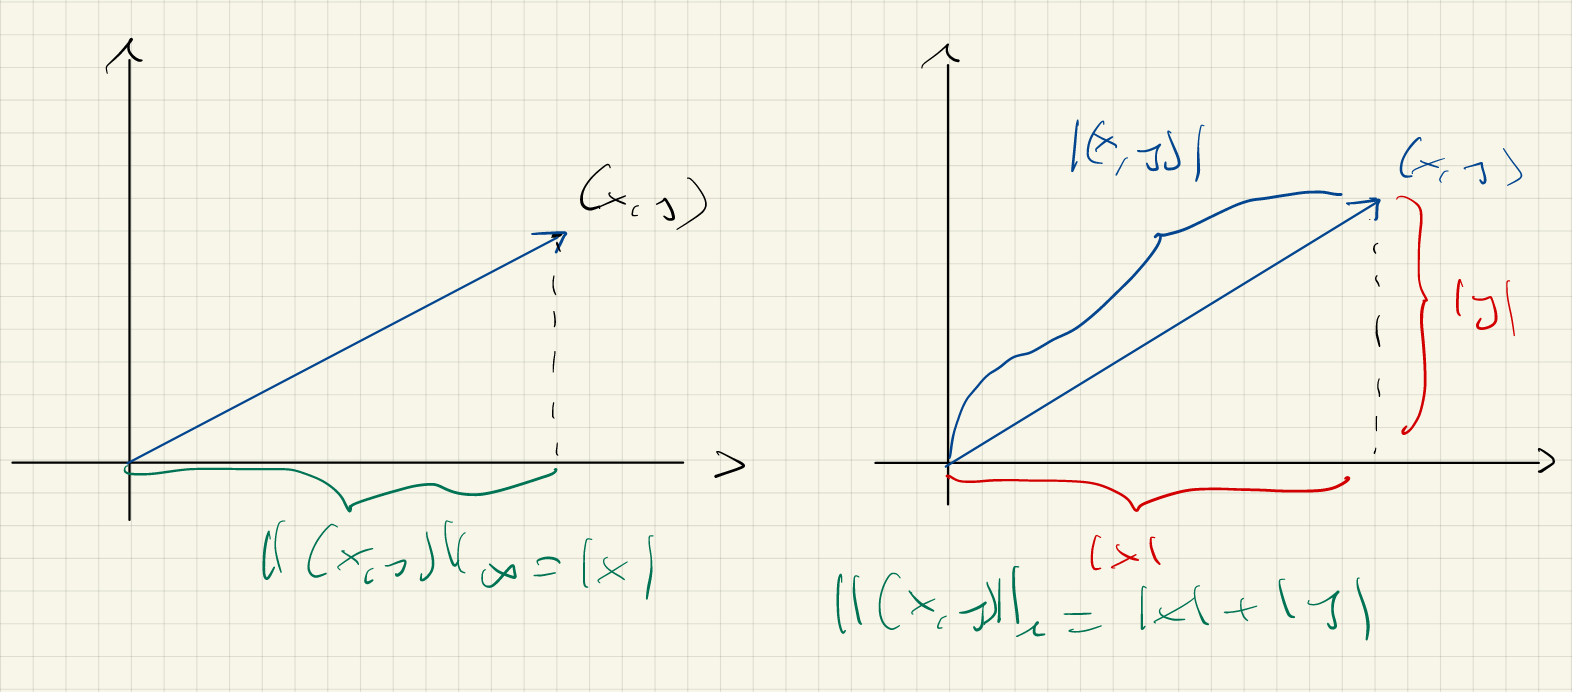
\includegraphics[width=\textwidth]{Screenshot from 2023-03-22 16-09-06.png}
\end{figure}
$\parallel\overline{x}\parallel_p = \left( \sum_{i=1}^{n}|x_i|^p \right)^{\frac{1}{p}},\,\,\, p \geq 1$\\
$\parallel\overline{x}\parallel_\infty = \lim_{p \rightarrow +\infty} \parallel\overline{x}\parallel_p$\\
$(\R^n,||\cdot||_p)$ è spazio normato

\begin{itemize}
    \item $C^\circ([0,1])$\\
    $\parallel f\parallel_\infty = \sup_{x \in [0,1]} |f(x)| \textcolor{orange}{(=\max_{x \in [0,1]} |f(x)|)}$\\
    $\parallel f\parallel_1=\int_{0}^{1} |f(x)|dx$\\
    $\parallel f\parallel_p= \left( \int_{0}^{1} |f(x)|^p dx\right)^{\frac{1}{p}}\,\,\,\, p \geq 1$\\
    sono tute norme su $C^\circ([0,1])$
\end{itemize}
Faccio vedere che $\parallel\cdot\parallel_\infty$ su $C^\circ([0,1])$ è una norma
\begin{enumerate}
    \item $\parallel f\parallel_\infty \geq 0$ (banale)\\
          $\parallel f\parallel_\infty =  0 \Leftrightarrow \sup_{x \in [0,1]}|f(x)|=0 \Leftrightarrow 0 \leq |f(x)| \leq0 \,\,\, \forall x \in[0,1] \Leftrightarrow f(x)=0\,\,\, \forall x\in[0,1]$
    \item $\parallel \lambda f\parallel_\infty = |\lambda|\parallel f\parallel_\infty \forall \lambda \in \R$ e $\forall f \in C^\circ([0,1])$\\
         $\parallel \lambda f\parallel_\infty = \sup_{x \in[0,1]}|\lambda f(x)|=\sup_{x\in[0,1]}|\lambda||f(x)|=|\lambda|\sup_{x\in[0,1]}|f(x)|=|\lambda|\parallel f\parallel_\infty$
    \item $\parallel f+g\parallel_\infty \leq \parallel f\parallel_\infty + \parallel g\parallel_\infty \,\,\, \forall f,g \in C^\circ([0,1])$\\
          $\parallel f+g\parallel_\infty = \sup_{x\in[0,1]} |f(x)+g(x)|$\\
          $|f(x)+g(x)| \leq |f(x)|+|g(x)|\leq \sup_{y\in[0,1]} |f(y)|+\sup_{y\in[0,1]} |g(y)|= \parallel f\parallel_\infty + \parallel g\parallel_\infty \,\,\, \forall x \in [0,1]$\\
          $\parallel f+g\parallel_\infty = \sup_{x\in[0,1]} |f(x)+g(x)|\leq \parallel f\parallel_\infty + \parallel g(x)\parallel_\infty$\\
\end{enumerate}
Facciamo vedere che $\parallel f\parallel_1 = \int_{0}^{1}|f(x)|dx$ è una norma
\begin{enumerate}
    \item $\parallel f \parallel_1 \geq 0\,\,\, \forall f\in C^\circ([0,1]) banale$\\
    Dimostriamo che $\parallel f \parallel_1=0 \Leftrightarrow f(x)=0\,\,\, \forall x\in[0,1]$\\
    $\Leftarrow) f(x)=0\,\,\, \forall x \in[0,1]$\\
    $\parallel f \parallel_1 =\int_{0}^{1}0dx=0$\\
    $\Rightarrow)$ Sia $\parallel f\parallel_1=0$ e dimostriamo che $f(x)=0\,\,\, \forall x \in [0,1]$\\
    $\int_{0}^{1}|f(x)|dx=0$\\
    Se $\exists x_0 \in [0,1]$ tale che $|f(x_0)|\neq 0$ allora $\exists$ un intorno $U$ di $x_0 $ tale che $|f(x)| \geq \frac{|f(x_0)|}{2}$ $\forall x \in U \cap [0,1]$ 
        \begin{itemize}
            \item $U=]x_0-\delta, x_0+\delta[ \subseteq [0,1]$
            \item $x_0=0$\\ $U=]0-\delta,0+\delta[$\\
                  $U \cap [0,1]=[0,\delta[$
            \item $x_1=1$\\ $U=]1-\delta,1+\delta[$\\
            $U \cap [0,1]=]1-\delta,1]$
        \end{itemize}
        cioè in ogni caso $U \cap [0,1]$ è un intervallo di ampiezza almeno $\frac{\delta}{2}>0$\\
        $\parallel f\parallel_1=\int_{0}^{1} |f(x)|dx \geq \int_{U \cap [0,1]} |f(x)|dx \geq \int_{U\cap [0,1]} \frac{|f(x_0)|}{2}dx \geq \frac{\delta}{4}|f(x_0)|>0$\\
        il che è assurdo, perchè $\parallel f\parallel_1=0$
    \item $\parallel \lambda f\parallel_1=\int_{0}^{1}|\lambda f(x)|dx= |\lambda|\int_{0}^{1}|f(x)|dx = |\lambda|\parallel f\parallel_1\,\,\,\, \lambda\in \R$
    \item $f,g \in C^\circ([0,1])$\\
        $||f+g||_1=\int_{0}^{1}|f(x)+g(x)|dx \leq \int_{0}^{1}(|f(x)|+|g(x)|)dx = ||f||_1+||g||_1 \Rightarrow$ vale la disuguaglianza triangolare
\end{enumerate}
Dato uno spazio normato $(X,\parallel\cdot\parallel)$ posso definire la distanza tra due vettori $x,y \in X$ come $d(x,y)= \parallel x-y\parallel$, lunghezza del vettore $x-y$.

\begin{figure}[h!]
    \centering
    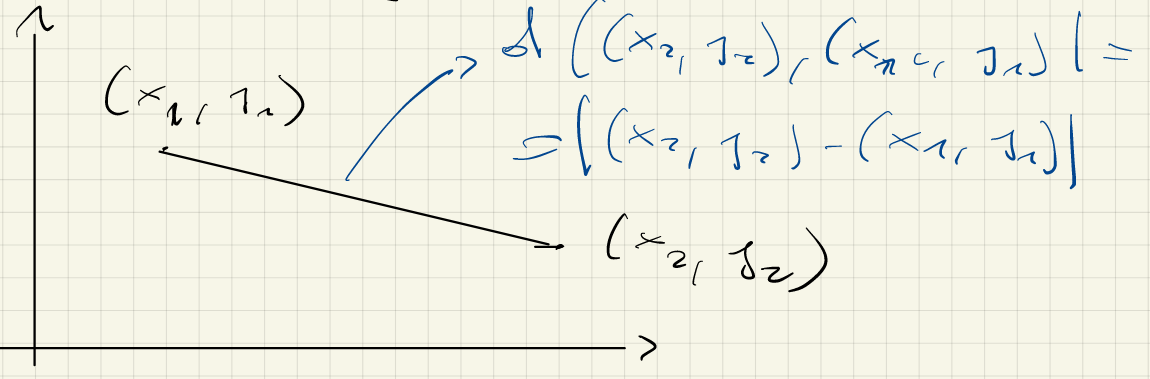
\includegraphics[width=\textwidth]{Screenshot from 2023-03-22 16-56-15.png}
\end{figure}

\paragraph{\textcolor{red}{Definizione}}
$X$ insieme non vuoto. Una distanza o metrica su $X$ è una funzione $d:X \times X\rightarrow \R$ tale che
\begin{enumerate}
    \item $d(x,y)\geq 0 \,\,\, \forall x,y \in X $ e $d(x,y)=0 \Leftrightarrow x=y$
    \item $d(x,y)=d(y,x)$ proprietà simmetrica
    \item Disuguaglianza triangolare $d(x,y)\leq d(x,z)+d(z,y) \,\,\, \forall x,y,z \in X$
\end{enumerate}
La coppia $(X,d)$ si dice \textcolor{red}{spazio metrico}.


\newpage
\section{\textcolor{red}{Lezione 11 \space\space 21/03/'23}}
\paragraph{\textcolor{red}{}}
$(X,\parallel\cdot\parallel)$ normato\\
$d(x,y)=\parallel x-y\parallel$ è metrica, allora
\begin{enumerate}
    \item $d(x,y)\geq 0$ banalmente\\
          $d(x,y)=\parallel x-y\parallel =0 \Leftrightarrow x-y=0 \Leftrightarrow x=y$
    \item$d(x,y)= \parallel x-y\parallel=\parallel y-x\parallel =d(y,x)$
    \item $d(x,y)=\parallel x-y\parallel=\parallel(x-z)+(z-y)\parallel\leq \parallel x-z\parallel+\parallel z-y\parallel=d(x,z)+d(y,z)$
\end{enumerate}
Dato uno spazio vettoriale $X$ e $d$ metrica su $X$, esiste una norma $\parallel\cdot\parallel$ su $X$ tale che $d(x,y)=\parallel x-y\parallel$?\\
No, esistono metriche dentro lo spazio vettoriale che non derivano da una norma.

\paragraph{\textcolor{red}{Esempio}}
$\R, \,\,\, 0 <p<1,\,\,\, d(x,y)=|x-y|^p$. Allora $d$ è una metrica, che non deriva da una norma.\\
Se esistesse una norma $\parallel\cdot\parallel$ su $\R$ tale che $d(x,y)=\parallel x-y\parallel$, allora, fissato $\lambda\in\R$,\\
$d(\lambda x,\lambda y)=\parallel\lambda x-\lambda y\parallel=|\lambda| \parallel x-y\parallel=|\lambda|d(x,y)$\\
$d(\lambda x,\lambda y)=|\lambda x-\lambda y|^p=|\lambda|^p|x-y|^p=|\lambda|^p d(x,y)\neq |\lambda|d(x,y)$ se $|\lambda \neq 1,0|$\\
Facciamo vedere che $d(x,y)=|x-y|^p$ è una distanza, $0<p<1$
\begin{enumerate}
    \item $d(x,y)\geq 0$ banale\\
    $d(x,y)=0 \Leftrightarrow |x-y|^p=0 \Leftrightarrow |x-y|=0 \Leftrightarrow x=y$
    \item $d(x,y)=d(y,x)$ banale
    \item Disuguaglianza triangolare\\
    Dobbiamo dimostrare che $\forall x,y,z \in \R$ vale\\
    $d(x,y)\leq d(x,z)+d(z,y)$\\
    $|x-y|^p\leq |x-z|^p+|z-y|^p$\\
    $|x-y|^p\leq (|x-z|+|y-z|)^p$ \textcolor{orange}{disuguaglianza triangolare per $|\cdot|$}\\
    Se dimostro che $(|x-z|+|y-z|)^p \leq |x-z|^p+|z-y|^p$, sono a posto $\forall x,y,z \in \R$ con $0<p<1$.\\
    Devo dunque dimostrare che $(a+b)^p\leq a^p+b^p \,\,\, \forall a,b\in\R^+$.\\
    Se $a=0$ o $b=0$, banale\\
    Siano $a,b\neq 0$\\
    $(a+b)^p\leq a^p+b^p\,\,\,\, /.\frac{1}{b^p}$\\
    $\Leftrightarrow \frac{(a+b)^p}{b^p}\leq \frac{a^p}{b^p}+1 \Leftrightarrow \left( \frac{a+b}{b} \right)^p \leq \left( \frac{a}{b} \right)^p +1 \Leftrightarrow \left( \frac{a}{b} +1 \right)^p \leq \left( \frac{a}{b} \right)^p +1 \,\,\, \forall a,b >0$\\
    Posto $\lambda = \frac{a}{b}>0$\\
    $\left( \frac{a}{b}+1 \right)^p \leq \left( \frac{a}{b} \right)^p +1\,\,\, \forall a,b>0 \Leftrightarrow (\lambda+1)^p\leq \lambda^p +1 \,\,\, \forall \lambda>0$\\
    $(\lambda+1)^p-\lambda^p\leq 1$\\
    $f(\lambda)=(\lambda +1)^p-\lambda^p\,\,\,\,\,\,f:\R^+\rightarrow\R$\\
    $f(\lambda)\leq 1=f(0)$\\
    $f'(\lambda)=p(\lambda+1)^{p-1}-p\lambda^{p-1}=p[(\lambda+1)^{p-1}-\lambda^{p-1}]=p\lambda^{p-1}\left[\left( \frac{\lambda+1}{\lambda} \right)^{p-1}-1\right]= p\lambda^{p-1} \left[ \left( 1+\frac{1}{\lambda} \right)^{p-1} -1\right] = <0\,\,\, \forall\lambda >0$\\
    $f$ è decrescente e quindi $\forall \lambda>0 \Rightarrow f(\lambda)\leq f(0)$, come si voleva.
\end{enumerate}

\subsection{\textcolor{red}{Topologia}}
$(x,d)$ spazio metrico.

\paragraph{\textcolor{red}{Definizione}}
Sia $x\in X, r >0$, allora $B_r(x)=\{ y\in x|d(x,y) < r \}$ si dice \textcolor{red}{palla (aperta)} di centro $x$ e raggio $r$.

\paragraph{\textcolor{red}{Esempi}}
$(\R^2,|\cdot|)$, $\R^2$ con norma euclidea\\
$B_r(0,0), r>0$\\
$B_r(0,0)=\{ (x,y)\in \R^2 |d((x,y),(0,0))<r \}=\{ (x,y)\in \R^2 | |(x,y)-(0,0)| <r \}=\{ (x,y)\in \R^2 | \sqrt{x^2+y^2} <r\}$
\begin{figure}[h!]
    \centering
    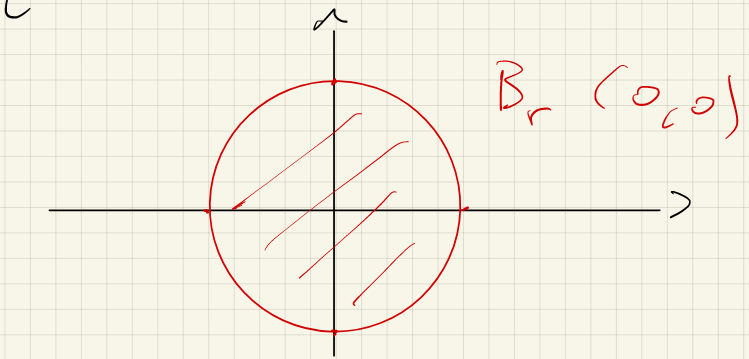
\includegraphics[width=0.5\textwidth]{Screenshot from 2023-03-22 17-44-33.png}
\end{figure}

Prendiamo $(\R^2,\parallel\cdot\parallel_\infty)$\\
$\parallel(x,y)\parallel_\infty= \max\{|x|,|y|\}$\\
$B_r^\infty (0,0)=\{ (x,y)\in \R^2| \parallel(x,y)-(0,0) \parallel_\infty <r\}=\{ (x,y)\in \R^2| \max\{|x|,|y|\}<r\}= \{ (x,y)\in \R^2| |x|,|y| <r\}$
\begin{figure}[h!]
    \centering
    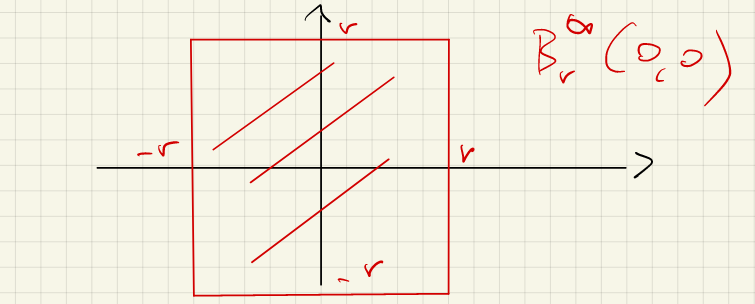
\includegraphics[width=0.5\textwidth]{Screenshot from 2023-03-22 17-45-00.png}
\end{figure}

Prendiamo $(\R^2,\parallel \cdot\parallel_1)$\\
$\parallel(x,y)\parallel_1=|x|+|y|$\\
$B_r^1 (0,0) =\{(x,y)\in \R^2 | \parallel (x,y)-(0,0) \parallel_1 <r \} =\{(x,y)\in \R^2 | |x|+|y| <r \}$
\begin{figure}[h!]
    \centering
    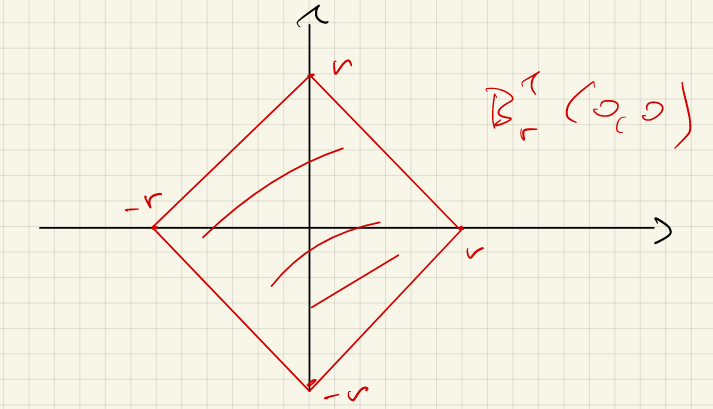
\includegraphics[width=0.5\textwidth]{Screenshot from 2023-03-22 17-45-31.png}
\end{figure}

($C^\circ([0,1]),\parallel\cdot\parallel_\infty$)\\
$d(f,g)=\parallel f-g\parallel_\infty$\\
$f\in C^\circ(),\,\,\, r>0$\\
$B_r^\infty(f)=\{ g\in C^\circ([0,1])| \parallel f-g\parallel_\infty < r \}=\{ g\in C^\circ([0,1])| \sup_{x\in[0,1]} |f(x)-g(x)|<\}$\\
\begin{figure}[h!]
    \centering
    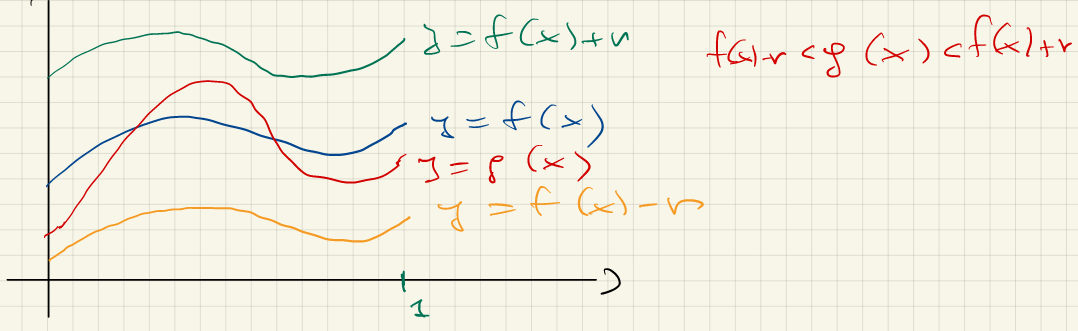
\includegraphics[width=0.5\textwidth]{Screenshot from 2023-03-22 17-45-52.png}
\end{figure}

$f(x)=0 \,\,\, \forall x \in [0,1]$\\

\begin{figure}[h!]
    \centering
    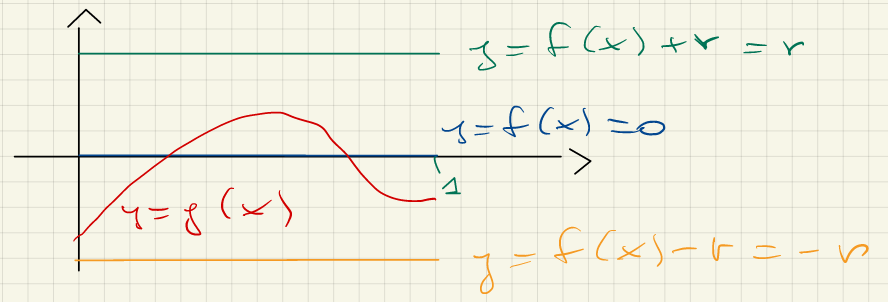
\includegraphics[width=0.5\textwidth]{Screenshot from 2023-03-22 17-46-13.png}
\end{figure}

$C^\circ([0,1]),\parallel\cdot\parallel_1$\\
$\parallel f\parallel_1=\int_{0}^{1}|f(x)|dx$\\
$B_r^1=\{ g\in C^\circ([0,1])| \parallel f-g\parallel_1 <r \}=\{g\in C^\circ([0,1])| \int_{0}^{1}|f(x)-g(x)|dx <r\}$\\
$f(x)=0\,\,\,\forall x \in [0,1]$\\
$B_r^1(0)=\{ g \in C^\circ([0,1])| \int_{0}^{1}|g(x)|dx <r \}$\\
\begin{figure}[h!]
    \centering
    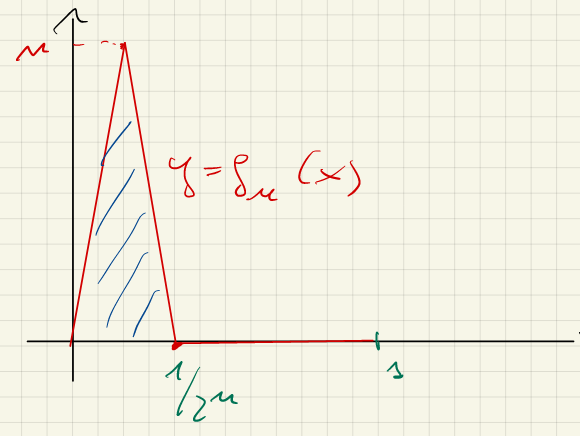
\includegraphics[width=0.5\textwidth]{Screenshot from 2023-03-22 17-46-35.png}
\end{figure}
$\int_{0}^{1}|g_n(x)|dx=$area del triangolo$= \frac{1}{2}\frac{1}{2^n}n=\frac{n}{2^{n+1}}$\\
Fissato $r>0$, trovo $n$ tale che $\int_{0}^{1}|g_n(x)|dx<r$

\paragraph{\textcolor{red}{Definizione}}
$x\in X$. Un \textcolor{red}{intorno di $x$} è un qualsiasi sottoinsieme $A \subseteq X$ che contiene una palla aperta centrata in $x$, cioè per cui $\exists r >0 | B_r(x)\subseteq A.$

\paragraph{\textcolor{red}{Definizione}}
$A \subseteq X$ si dice \textcolor{red}{aperto} se è intorno di ogni suo punto, cioè se $\forall x \in A\,\,\, \exists r>0\,\,|\,\, B_r(x)\subseteq A$.\\
$A$ si dice \textcolor{red}{chiuso} se $A^c = X \backslash A$ è aperto.

\paragraph{\textcolor{red}{Esempio}}
$(x,d)$ spazio metrico, $x \in X, r>0$, $B_r(x)$ è un aperto.\\
Devo far vedere che $\forall y \in B_r(x)\,\, \exists\,\, \overline{r}>0\,\,|\,\,B_{\overline{r}}(y)\subseteq B_r(x)$\\
$\overline{r}=r-d(x,y)>0$ perchè $d(x,y)<r$ e dimostriamo che, se $z \in B_{\overline{r}}(y)$, allora $z\in B_r(x)$, cioè, se $d(y,z)< \overline{r}$, allora $d(x,z)<r$\\
$d(x,z)\leq d(x,y)+d(y,z)<d(x,y)+\overline{r}=d(x,y)+(r-d(x,y))=r$
\begin{figure}[h!]
    \centering
    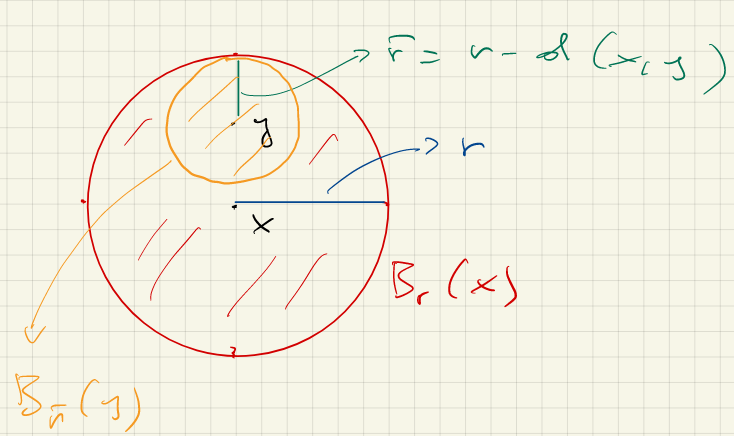
\includegraphics[width=0.5\textwidth]{Screenshot from 2023-03-22 17-46-52.png}
\end{figure}

\paragraph{\textcolor{red}{Esempio}}
$(\R^2,\parallel\cdot\parallel_\infty)$
\begin{figure}[h!]
    \centering
    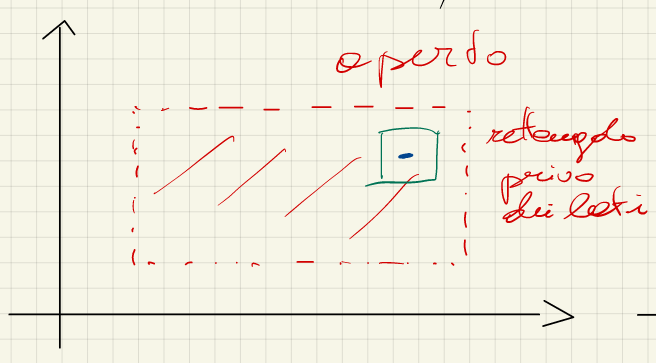
\includegraphics[width=0.48\textwidth]{quad1.png} 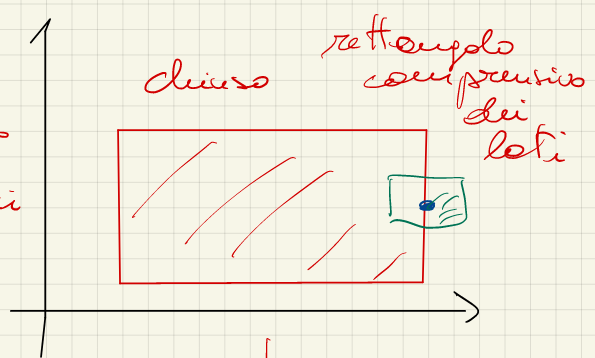
\includegraphics[width=0.48\textwidth]{quad2.png} \\[\smallskipamount]
    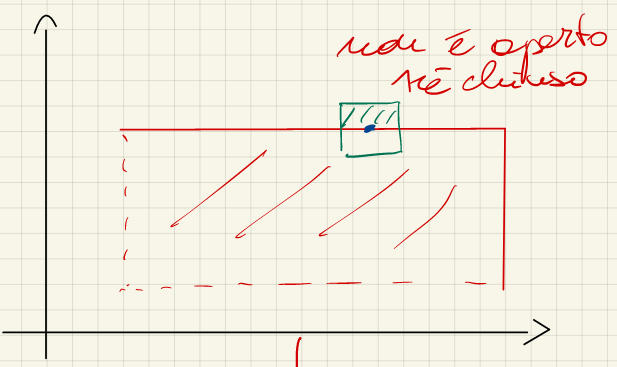
\includegraphics[width=0.48\textwidth]{quad3.png} 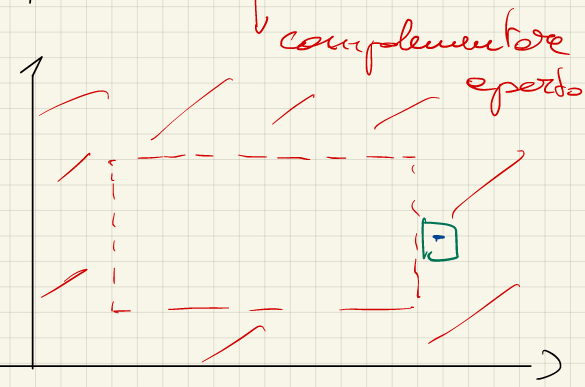
\includegraphics[width=0.48\textwidth]{quad4.png} \\[\smallskipamount]
    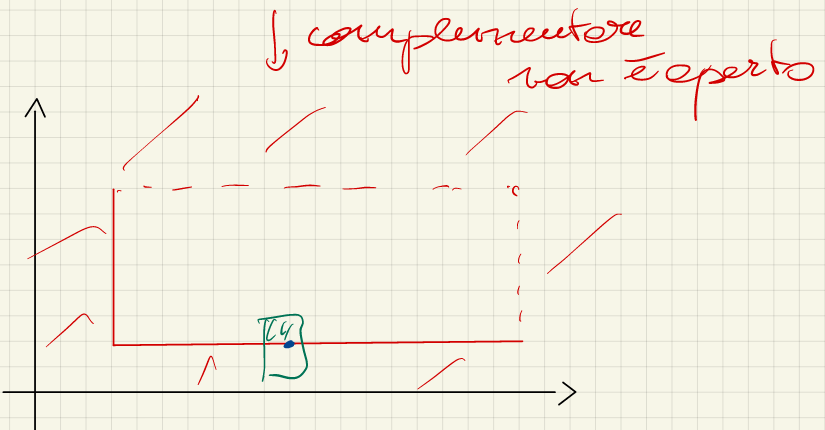
\includegraphics[width=0.48\textwidth]{quad5.png}
\end{figure}

\paragraph{\textcolor{red}{Osservazione}}
$(X,d)$ spazio metrico, $X$ è aperto banalmente \textcolor{orange}{(se $x\in X, B_r(x) \subseteq X \forall r>0$)} e quindi $\emptyset = X^c = X \backslash X$ è chiuso. D'altra parte $\emptyset $ è aperto perchè l'implicazione $x \in \emptyset \Rightarrow \exists r >0 | B_r(x) \subseteq \emptyset$ è vera perchè $x \in \emptyset$  è falsa $\Rightarrow \emptyset^c=X \backslash \emptyset = X$ è chiuso. $\emptyset, X$ sono sia aperti che chiusi.

\paragraph{\textcolor{red}{Teorema}}
$(X,d)$ spazio metrico
\begin{enumerate}
    \item $A_1,A_2 \subseteq X$ aperti $\Rightarrow A_1 \cap A_2$ è un aperto. 
    \item $\{A_i\}_{i\in I}$ è una famiglia di aperti, allora $\bigcup_{i\in I}A_i$ è un aperto.
    \item Se $C_1,C_2 \subseteq X$ sono chiusi, allora $C_1 \cup C_2$ è chiuso.
    \item $\{C_i\}_{i\in I}$ è famiglia di chiusi, allora $\bigcap_{i\in I} C_i$ è un chiuso.
\end{enumerate}

\paragraph{\textcolor{red}{Osservazione}}
In generale se $\{ a_i\}_{i\in I}$ è una famiglia infinita di aperti, allora $\bigcap_{i\in I} A_i$ non è un aperto e, se $\{C_i\}_{i \in I}$ è una famiglia infinita di chiusi, allora $\bigcup_{i\in I} C_i$ non è chiuso. Facciamo un esempio.\\
$A_k=]-\frac{1}{k},\frac{1}{k}[,\,\,\, k \geq 1, k \in \N$ sono tutti aperti di $\R$, allora $\bigcap_{k=1}^\infty A_k = \bigcap_{k=1}^\infty ]-\frac{1}{k},\frac{1}{k}[=\{0\}$, che è un chiuso.\\
$C_k=[\frac{1}{k},1-\frac{1}{k}], k \geq 2, k \in \N$ sono tutti chiusi \textcolor{orange}{($C_k^c=]-\infty,\frac{1}{k}[\cup]1-\frac{1}{k},+\infty[$, unione di due intervalli aperti)}\\
$\bigcup_{k=2}^\infty C_k = \bigcup_{k=2}^\infty \left[\frac{1}{k},1-\frac{1}{k}\right]=]0,1[$\
Infatti, se $x \in \bigcup_{k=2}^\infty [\frac{1}{k},1-\frac{1}{k}]$, allora $\exists \overline{k} \geq 2 | \left[\frac{1}{k},1-\frac{1}{k}\right]$, cioè $0<\frac{1}{k}\leq x \leq 1- \frac{1}{k}< 1 \Rightarrow 0<x<1 \Rightarrow x \in ]0,1[.$\\
D'altra parte, se $x \in ]0,1[$, esistono $k_1$ e $k_2$ tali che $\frac{1}{k_1}<x<1-\frac{1}{k_2}$ e se $k=\max\{k_1,k_2\}$ allora\\
$\frac{1}{k}\leq \frac{1}{k_1} <x<1-\frac{1}{k_2}\leq 1-\frac{1}{k}$\\
$\Rightarrow x\in C_k =[\frac{1}{k},1-\frac{1}{k}]$\\
$\Rightarrow x\in \bigcup_{k=2}^{\infty} C_k$.

\paragraph{\textcolor{red}{Definizione}}
$(X,d)$ spazio metrico, $A \subseteq X$, $x \in A$. $x$ si dice \textcolor{red}{punto interno di A} se $\exists r>0 |B_r(x)\subseteq A$. L'interno di $A$ è l'insieme dei punti interni di $A$ ed è indicato con $\AA$

\paragraph{\textcolor{red}{Proposizione}}
$\AA$ è un insieme aperto ed è il più grande aperto, nel senso dell'inclusione, contenuto in $A$, cioè se $B \subseteq A$ è aperto, allora $B \subseteq \AA$

\paragraph{\textcolor{red}{Dimostrazione (Esercizio per casa)}}

\paragraph{\textcolor{red}{Esempio}} 
$A=]0,1], \,\,\,\,\, \AA =]0,1[$\\
$A=]0,1] \cup \{2\}, \,\,\,\,\,\, \AA =]0,1[$\\
$A=]0,1]\cup \{2+\frac{1}{n}|n \geq 1, n \in \N\},\,\,\,\,\,\AA = ]0,1[$

\paragraph{\textcolor{red}{Definizione}}
$A \subseteq X, x \in X$ si dice punto di \textcolor{red}{chiusura} per $A$ se $B_r(x) \cap A \neq \emptyset \forall r>0$, cioè ogni palla di centro $x$ interseca $A$. La chiusura di $A$ è l'insieme di tutti i punti di chiusura di $A$ ed è denotata con $\overline{A}$.

\paragraph{\textcolor{red}{Proposizione}}
$\overline{A} $ è un insieme chiuso ed è il più piccolo chiuso, nel senso dell'inclusione, contenente $A$, cioè, se $C \geq A$ è chiuso, allora $\overline{A}\subseteq C$

\paragraph{\textcolor{red}{Dimostrazione (Esercizio per casa)}}
\paragraph{\textcolor{red}{Esempio}}
$A=]0,1],\,\,\,\, \overline{A}=[0,1]\\
A=]0,1]\cup \{2\}, \,\,\,\, \overline{A}=[0,1]\cup \{2\}\\
A=]0,1]\cup \{ 2+\frac{1}{n}|n \geq 1, n \in \N \}, \,\,\,\,\, \overline{A}=[0,1] \cup \{2+\frac{1}{n}|n \geq 1, n \in \N \} \cup \{2\}  $

\paragraph{\textcolor{red}{Osservazione}}
$\AA \subseteq A \subseteq \overline{A}$\\
$A $ è aperto $\Leftrightarrow A= \AA$\\
$A$ è chiuso $\Leftrightarrow A=\overline{A}$\\
\textcolor{orange}{$\Leftarrow) A=\overline{A}$, $\overline{A}$ è un chiuso$\Rightarrow A$ è chiuso $\Rightarrow)$ Sia $A$ chiuso e dimostriamo che $A=\overline{A}$. Noi sappiamo che $A \subseteq \overline{A}$ quindi, see per assurdo $A \nsubseteq \overline{A}, \exists x \in \overline{A}| x \notin A$, cioè $x \in \overline{A}$ e $x \in A^c$. Ma $ A^c $ è aperto, perchè $ A $ è chiuso, e quindi $ \exists r >0 $ tale che $ B_r (x) \subseteq A^c \Rightarrow B_r (x) \cap A = \emptyset$, assurdo perche $x \in \overline{A}$ .}

\paragraph{\textcolor{red}{Definizione}}
$A \subseteq X, x \in X$ si dice \textcolor{red}{punto di frontiera} per $A$ se $\forall r>0 \,\,\, B_r(x) \cap A \neq \emptyset$ e $B_r(x) \cap A^c \neq \emptyset$, cioè se ogni palla di centro $x$ interseca sia $A$ che il suo complementare.\\
L'insieme dei punti di frontiera di $A$ si dice frontiera di $A$ e si indica con $\partial A$. 

\paragraph{\textcolor{red}{Esempi}}
$A=]0,1],\,\,\,\, \partial A= \{0,1\}$\\
$A=]0,1]\cup\{2\},\,\,\,\,\, \partial A= \{0,1,2\}$\\
$A=]0,1]\cup \{ 2+\frac{1}{n}|n \geq 1, n \in \N \}, \,\,\,\,\, \partial A =\{0,1\}\cup \{2+\frac{1}{n}|n \geq 1, n \in \N \} \cup \{2\}$

\begin{figure}[h!]
    \centering
    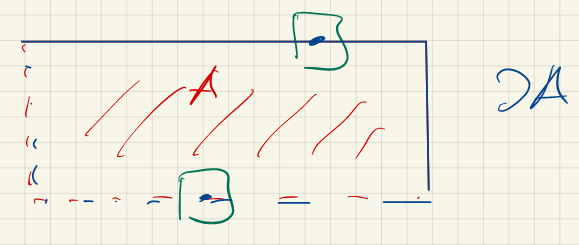
\includegraphics[width=0.5\textwidth]{Screenshot from 2023-03-22 17-49-55.png}
\end{figure}

\newpage
\section{\textcolor{red}{Lezione 12 \space\space 23/03/'23}}

\paragraph{\textcolor{red}{Osservazione}}
\begin{itemize}
    \item $\partial A = \overline{A} \cap \overline{A^c}$, $x \in \partial A$\\
        $\Rightarrow B_r (x)\cap A \neq \emptyset \,\,\, \forall r>0$, $x\in \overline{A}$\\
        $\Rightarrow B_r(x)\cap A^c \neq \emptyset \,\,\,\forall r>0$, $x\in \overline{A^c}$\\
        $\Rightarrow x \in \overline{A} \cap \overline{A^c} \Rightarrow \partial A \subseteq \overline{A} \cap \overline{A^c}$\\
        $x\in\overline{A}\cap \overline{A^c} \Rightarrow x\in \overline{A} $ e $x \in \overline{A^C}$\\
        $x \in \overline{A} \Rightarrow B_r(x)\cap A\neq \emptyset\,\,\, \forall r>0$\\
        $x \in \overline{A^c} \Rightarrow B_r(x)\cap A^c \neq \emptyset\,\,\, \forall r>0$\\
        $\Rightarrow x\in \partial A \Rightarrow \overline{A} \cap \overline{A^c} \subseteq \partial A$
    \item $\overline{A}=A \cup \partial A$\\
        $A \subseteq \overline{A}$, $\partial A \subseteq \overline{A} \Rightarrow A \cup \partial A \subseteq \overline{A}$\\
        Facciamo vedere che $\overline{A}\subseteq A \cup \partial A$.\\
        $x\in \overline{A}$, supponiamo che $x\notin A$ e dimostriamo che $x \in \partial A$\\
        $x\in \overline{A}  \Rightarrow B_r(x)\cap A \neq \emptyset \,\,\, \forall r>0$\\
        $x \in B_r (x)\cap A^c \,\,\,\forall r >0$\\
        $B_r(x)\cap A^c \neq \emptyset \,\,\, \forall r>0$\\
        $\Rightarrow x\in \partial A$, come si voleva
\end{itemize}

\paragraph{\textcolor{red}{Osservazione}}
$A$ è chiuso $\Leftrightarrow \partial A \subseteq A$, cioè se e solo se $A$ contiene la sua frontiera.

\paragraph{\textcolor{red}{Esempio}}
$(\R, |\cdot|), \Q \subseteq \R$\\
Si ha che $\overline{\Q}=\R$.\\
Fissati $x\in \R$ e $ r>0 $ $ \exists q \in \Q $ tale che $ q\in ]x-r,x+r[=B_r(x)$.\\
Si ha anche che $\partial \Q = \R$.\\
$x \in \R, B_r(x)\cap \Q \neq \emptyset \,\,\, \forall r>0, B_r(x)\cap \Q^c \neq \emptyset \,\,\, \forall r >0 $\\
$]x-r,x+r[\cap \Q^c \neq \emptyset \,\,\, \forall r>0$\\
Se non fosse vero, $\exists x \in \R$ e $r>0$ tale che $]x-r,x+r[$ è fatto tutto di numeri razionali.\\
\textcolor{orange}{I razionali sono numerabili, cioè $\exists f: \N\rightarrow \Q $ iniettiva e suriettiva. I reali hanno la potenza del continuo, cioè ogni funzione $\phi:\N\rightarrow\R$ può essere al più iniettiva, ma non suriettiva. Questo è vero anche per ogni intervallo del tipo $]x-r,x+r[, r>0$. Quindi, se $]x-r,x+r[$ fosse fatto di soli numeri razionali, sarebbe numerabile, assurdo.}

\subsection{\textcolor{red}{Successioni in spazi metrici}}
\paragraph{}
\begin{itemize}
    \item $\R^2\,\,\,\,\,\,\, \{(e^{-n}, \frac{\sin n}{n}) \}_{n\geq 1}$ è una successione di elementi di $\R^2$
    \item $\R^3\,\,\,\,\,\,\, \{ (1+\frac{1}{n}, \frac{\sinh n}{e^n},2^{-n}) \}$ è una successione di elementi di $\R^3$
\end{itemize}


\paragraph{\textcolor{red}{Definizione}}
$\{x_k\}_{k\in \N} \subseteq X$ successione, con $(X,d)$ spazio metrico. Si dice che $\{ x_k\}_{k\in\N}$ converge ad $x \in X$ e si scrive
\begin{empheq}{equation*}
x_k \rightarrow x \,\,\,\,\, \text{o} \,\,\,\,\,\lim_{k\rightarrow +\infty} x_k = x \Leftrightarrow \lim_{k \rightarrow +\infty} d(x_k,x)=0
\end{empheq}
\textcolor{orange}{(in ambito reale $\lim_{k \rightarrow+\infty} |x_k - x |=0$)}\\
cioè $\Leftrightarrow \forall \,\, \epsilon >0 \,\, \exists\,\, N >0 $ tale che $k > N \Rightarrow d(x_k,x)<\epsilon$\\
$x$ viene detto limite della successione.

\paragraph{\textcolor{red}{Teorema}}
Sia $\{ x_k \}_{k \in \N} \subseteq X, (X,d)$ spazio metrico, tale che $ x_k \rightarrow l_1 \in X$ e $x_k \rightarrow l_2 \in X$. Allora $l_1=l_2$.

\paragraph{\textcolor{red}{Proposizione}}
$\{\overline{x_k}\}_{k\in\N} \subseteq R^n$ tale che $\overline{x_k } = (x_{k_1},x_{k_2},...,x_{k_n})$. Allora $\overline{x_k}\rightarrow \overline{x}=(x_1,...,x_n) \Leftrightarrow x_{kj} \rightarrow x_j \,\,  \forall \,\, j=1,...,n$ cioè $\Leftrightarrow \forall \,\, j = 1,...,n$ la successione di numeri reali $\{ x_{kj}\}_{k\in\N}$ converge a $x_j$.

\paragraph{\textcolor{red}{Esempi}}
\begin{itemize}
    \item $\R^2, \{(e^{-k}, \frac{\sin k}{k})\}_{k \geq 1}$\\
        $\overline{x_k}=(x_{k_1},x_{k_2}), \,\,\, x_{k_1}=e^{-k}, \,\,\, x_{k_2}=\frac{\sin k}{k}$\\
        $\lim_{k \rightarrow +\infty} x_{k_1}=0, \,\,\, \lim_{k \rightarrow +\infty} x_{k_2}=0$\\
        $\Rightarrow \lim_{k \rightarrow + \infty} \overline{x_k} =(0,0)$
    \item -$\R^3, \{ a+\frac{1}{k}, \frac{\sinh k}{e^k}, \}_{k \geq 1}$\\
        $x_{k_1}=1+\frac{1}{k}, \,\,\, x_{k_2}=\frac{\sinh k}{e^k},\,\,\, x_{k_3}=2^{-k}$\\
        $\lim_{k \rightarrow +\infty}x_{k_1}=1, \,\,\, \lim_{k \rightarrow +\infty} x_{k_2}=1, \,\,\, \lim_{k \rightarrow +\infty} x_{k_3}=0 $\\
        $\lim_{k \rightarrow +\infty} \overline{x_k} =(1,1,0)$
    \item
        -$\R^2, \{(2+e^{-k}, \sin k)\} $\\
        $x_{k1}=2+e^{-k},\,\,\, x_{k2}=\sin k$\\
        $\lim_{k \rightarrow +\infty}x_{k_1}=2, \,\,\, \lim_{k \rightarrow +\infty}$ non esiste $\Rightarrow \lim_{k \rightarrow +\infty} \overline{x_k}$ non esiste.
\end{itemize}

\paragraph{\textcolor{red}{Dimostrazione della proposizione}}
$(\R^n, |\cdot|)$\\
Se $\overline{y}=(y_1,..,y_n)\in \R^n$, allora $|y_j|\leq |\overline{y}|\leq \sum_{i=1}^{n}|y_i| \forall j$\\
$|y_j| = \sqrt{|y_j|^2} \leq \sqrt{\sum_{i=1}^{n}|y_i|^2} = |\overline{y}|$.\\
Abbiamo dimostrato che, se $0 <p<1$, $(a+b)^p\leq a^p+b^p \,\, \forall\,\, a,b \geq 0$.\\
Questa disuguaglianza si può generalizzare.\\
$(a_1+a_2+...+a_n)^p\leq a_1^p+a_2^p+...+a_n^p \,\, \forall\,\, a_i \geq 0$\\
$|\overline{y}|=\sqrt{\sum_{i=1}^{n}|y_i|^2} \leq (|y_1|^2)^{\frac{1}{2}}+(|y_2|^2)^{\frac{1}{2}}+...+(|y_n|^2)^{\frac{1}{2}}= |y_1|+|y_2|+...+|y_n|= \sum_{i=1}^{n}|y_i|$\\
$|y_j|\leq |\overline{y}| \leq \sum_{i=1}^{n}|y_i|$\\
$\overline{x} \rightarrow \overline{x} \Leftrightarrow x_{k_j} \rightarrow x_j \,\, \forall\,\, j=1,...,n$\\
$|x_{k_j}-x_j|\leq |\overline{x_k}-\overline{x}| \leq \sum_{i=1}^{n}|x_{k_i}-x_i|$.\\
Se $|\overline{x_k} - \overline{x}|\rightarrow 0 $, cioè se $\overline{x_k}\rightarrow \overline{x}$, allora\\
$0 \leq |x_{kj}-x_j|\leq |\overline{x_k}-\overline{x}| \Rightarrow x_{kj} \rightarrow x_j \,\, \forall \,\, j$\\
D'altra parte, se $x_{ki} \rightarrow  x_i \,\, \forall \,\, i=1,...,n $\\
$\Rightarrow \sum_{i=1}^{n}|x_{k_i}- x_i| \rightarrow 0 $ per $k \rightarrow + \infty$\\
$\Rightarrow 0 \leq |x_{k}- x| \leq \sum_{i=1}^{n}|x_{k_i}- x_i| \Rightarrow \overline{x_k} \rightarrow \overline{x}$.
\begin{flushright}
\large\Lightning
\end{flushright}

\newpage
\section{\textcolor{red}{Lezione 13 \space\space 27/03/'23}}
\paragraph{\textcolor{red}{Teorema: caratterizzazione dei chiusi mediante le successioni}}
$(X,d)$ spazio metrico, $A \subseteq X$. Allora $z\in \overline{A}\Leftrightarrow \exists$ una successione $\{x_k\}_{k\geq 1} \subseteq A $ tale che $x_k \rightarrow z$.

\paragraph{\textcolor{red}{Corollario}}
$(X,d)$ spazio metrico. $A \subseteq X$ è chiuso $\Leftrightarrow \forall\,\, \{x_k\}_{k \geq 1} \subseteq A$ convergente, il suo limite appartiene ad $A$.\\
\textcolor{orange}{($A \subseteq X$ è chiuso $\Leftrightarrow A$ contiene i limiti delle successioni convergenti a valori in $A$.)}

\paragraph{\textcolor{red}{Dimostrazione del Corollario}}
\begin{itemize}
    \item $\Rightarrow)$ $A$ chiuso, $A = \overline{A}$. Sia $\{x_k\}_{k \geq 1} \subseteq A$ successione convergente a $z \in X$. Allora il teorema implica che $z \in \overline{A}= A$.
    \item $\Leftarrow ) $ Dobbiamo dimostrare che, se $x \in \overline{A}$, allora $z \in A$\\ \textcolor{orange}{($A=\overline{A}$, perchè l'inclusione $A \subseteq \overline{A}$ è nota)}\\
$z \in \overline{A} \Rightarrow \,\, \exists \{x_k\}_{k \geq 1} \subseteq A$ convergente a $z$. Allora $z \in A$ per ipotesi.
\end{itemize}
\begin{flushright}
\large\Lightning
\end{flushright}

\paragraph{\textcolor{red}{Dimostrazione del Teorema}}
\begin{itemize}
    \item $\Rightarrow ) $ Sia $z \in \overline{A}$. Costruiamo una successione $\{x_k\}_{k \geq 1} \subseteq A \,\,|\,\, x_k \rightarrow z, z\in \overline{A} \Leftrightarrow \forall r >0, B_r(z)\cap A \neq \emptyset$.\\
    $r=1\,\,\,\,\,\, \exists\,\, x_1 \in B_1(z) \cap A$, $x_1 \in A$ e $d(x_1,z)<1$\\
    $r=\frac{1}{2}\,\,\,\,\,\, \exists \,\,x_2 \in B_{\frac{1}{2}}(z) \cap A$, $ x_2 \in A $ e $ d(x_2,z)< \frac{1}{2}$\\
    ...\\
    $r=\frac{1}{k}\,\,\,\,\,\, \exists\,\, x_k \in B_{\frac{1}{k}}(z)\cap A$, $ x_k \in A $ e $ d(x_k,z)< \frac{1}{k}$\\
    $\{x_k\}_{k \geq 1} \subseteq A$ tale che $0 \leq d(x_k,z)\leq \frac{1}{k} \Rightarrow \lim_{k \rightarrow +\infty} d(x_k,z)=0 \Rightarrow x_k \rightarrow z$.
    \item $\Leftarrow )$ Ipotesi: $\exists \,\, \{x_k\}_{k\geq 1} \subseteq A$ tale che $x_k \rightarrow z$. Tesi: $z \in \overline{A}$.\\
    Sia $r >0$. Poichè $x_k \rightarrow z \,\, \exists \,\, N> 0$ tale che $d(x_k,z)<r\,\, \forall \,\, k > N, x_k \in B_r(z) \cap A$\\
    $ \Rightarrow B_r(z) \cap A \neq \emptyset \Rightarrow z \in \overline{A}$. 
\end{itemize}
\begin{flushright}
\large\Lightning
\end{flushright}

\paragraph{\textcolor{red}{Esempi}}
\begin{itemize}
    \item $\Q$ non è chiuso in  $\R$ perchè $\exists \,\, \{q_n\}_{n\geq 1} \subseteq \Q \,\,|\,\, q_n \rightarrow \sqrt{2} \neq \Q$
    \item $(\R, |\cdot|)$
\end{itemize}
    \begin{figure}[!h]
        \centering
        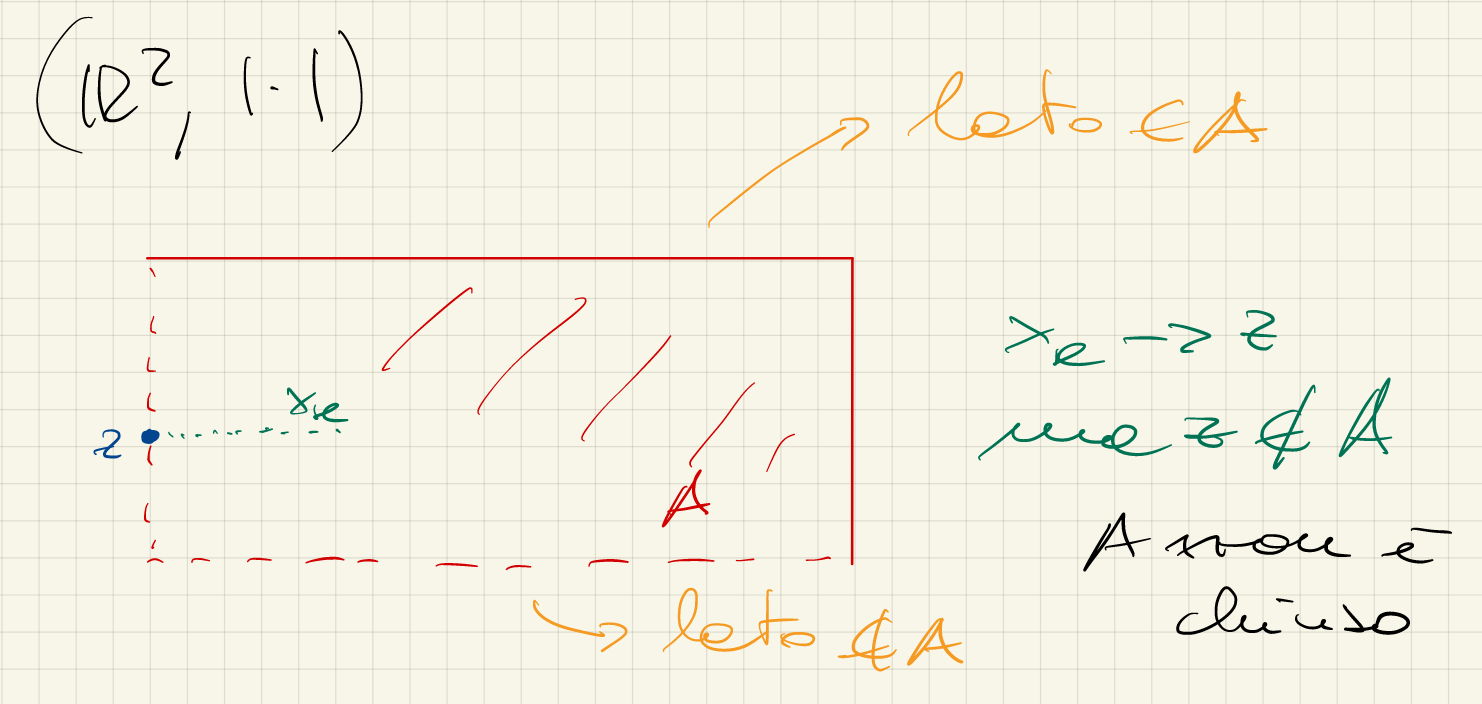
\includegraphics[width=0.5\textwidth]{Screenshot from 2023-03-28 18-09-08}
    \end{figure}

\paragraph{\textcolor{red}{Esempio importante}}
$C\subseteq \R^n$. Sono equivalenti le seguenti affermazioni
\begin{enumerate}
    \item $C$ è chiuso per la topologia data dalla norma euclidea $|\cdot|$
    \item $C$ è chiuso per la topologia data dalla norma $\parallel \cdot \parallel_\infty$
    \item $C$ è chiuso per la topologia data dalla norma $\parallel \cdot \parallel_1$
\end{enumerate}
Per dimostrare che le tre affermazioni sono equivalenti, partiamo da\\
$|x_j|\leq |\overline{x}| \leq \sum_{i=1}^{n}|x_i| \,\,\forall\,\, \overline{x}=(x_1,...,x_n)\in \R^n$\\
$\max_{j=1,...,n}|x_j| \leq |\overline{x}| \leq \sum_{i=1}^{n}|x_i| \leq n \max_{j=1,...,n}|x_j|$\\
\textcolor{red}{$\parallel \overline{x} \parallel_\infty \leq |\overline{x}| \leq \parallel \overline{x} \parallel_1 \leq n \parallel \overline{x} \parallel_\infty \forall\,\, \overline{x} \in \R^n$}
\begin{itemize}
    \item $1) \Rightarrow 2)$ Ipotesi: $C$ è chiuso per $|\cdot|$. Tesi: $C$ è chiuso per $ \parallel \cdot \parallel_\infty$\\
        $\{\overline{x_k}\}_{k\geq 1} \subseteq C \,\, |\,\, \overline{x_k} \rightarrow \overline{z}$ per $\parallel \cdot \parallel_\infty$, cioè $\parallel \overline{x_k}-\overline{z} \parallel_\infty \rightarrow 0 $ per $k \rightarrow +\infty$, e dimostriamo che $\overline{z} \in C$\\
        $|\overline{x_k}-\overline{z}|\leq n \parallel \overline{x_k}-\overline{z} \parallel_\infty \rightarrow 0$\\
        $\Rightarrow |\overline{x_k}-\overline{z}| \rightarrow 0$ per $k \rightarrow +\infty$, cioè $\overline{x_k} \rightarrow \overline{z}$ per $|\cdot|$. Ma $C$ è chiuso per $|\cdot| \Rightarrow \overline{z} \in \C$.
    \item $2) \Rightarrow 3)$ Ipotesi: $C$ è chiuso per $\parallel \cdot \parallel_\infty$.        Tesi: $C$ è chiuso per $\parallel \cdot \parallel_1$\\
        $\{\overline{x_k}\}_{k \geq 1} \subseteq C \,\,|\,\, \overline{x_k} \rightarrow \overline{z}$ per $\parallel \cdot \parallel_1$, cioè $\parallel \overline{x_k}-\overline{z} \parallel_1 \rightarrow 0$ per $k \rightarrow +\infty$ e dimostriamo che $\overline{z}\in C$.\\
        $\parallel \overline{x} \parallel_\infty \leq \parallel \overline{x} \parallel_1 \,\, \forall \,\, \overline{x}\in \R^n$\\
        Prendo $\overline{x} = \overline{x_k} -\overline{z}$\\
        $\parallel \overline{x_k} -\overline{z} \parallel_\infty \leq  \parallel\overline{x_k} -\overline{z} \parallel_1 \rightarrow 0 \Rightarrow \overline{x_k}  \rightarrow \overline{z}$ per $\parallel \cdot \parallel_\infty \rightarrow \overline{z} \in \C$ perchè $C $ è chiuso  per $\parallel\cdot\parallel_\infty$.
    \item $3) \Rightarrow 1)$ Ipotesi: $C$ è chiuso per $\parallel \cdot \parallel_1$. Tesi:       $C$ è chiuso per $|\cdot|$\\
        $\{ \overline{x_k}\}_{k \geq 1} \subseteq C \,\, | \,\, \overline{x_k} \rightarrow \overline{z}$ per $|\cdot|$ e dimostriamo che $\overline{z} \in C$ \\
        $\parallel \overline{x} \parallel_1 \leq n \parallel \overline{x} \parallel_\infty \,\, \forall \,\, \overline{x} \in \R^n$\\
        $\frac{1}{n} \parallel \overline{x} \parallel_1 \leq \parallel \overline{x}\parallel_\infty \leq |\overline{x}|\,\, \forall\,\, \overline{x} \in \R^n$\\
        $\parallel \overline{x}\parallel_1 \leq n |\overline{x}| \,\,\forall\,\, \overline{x} \in \R^n$\\
        $\overline{x}=\overline{x_k}-\overline{z}$\\
        $\Rightarrow \parallel \overline{x_k}-\overline{z}\parallel_1 \leq n |\overline{x_k}-\overline{z}| \rightarrow 0$ per $k \rightarrow +\infty$\\
        $\Rightarrow \parallel \overline{x_k}-\overline{z} \parallel_1 \rightarrow 0$ per $k \rightarrow +\infty$\\
        $\Rightarrow \overline{x_k}-\overline{z}$ per $\parallel \cdot \parallel_1 \Rightarrow z \in C$ perchè $C$ è chiuso per $\parallel \cdot \parallel_1$.
\end{itemize}
\begin{flushright}
\large\Lightning
\end{flushright}

\paragraph{\textcolor{red}{Osservazione}}
Siccome $C$ è chiuso $\Leftrightarrow C^c$ è aperto, il corollario al teorema che abbiamo appena dimostrato implica che $A \subseteq R^n$ è aperto per $|\cdot|  \Leftrightarrow A $ è aperto per la topologia data da $\parallel \cdot \parallel_\infty \Leftrightarrow A$ è aperto per $\parallel \cdot \parallel_1$, cioè le 3 norme $|\cdot|, \parallel \cdot \parallel_\infty, \parallel \cdot \parallel_1$ descirvono la stessa toplogia.\\
Si può dimostrare che in $\R^n$ \textcolor{red}{(spazio di dimensione finita)} tutte le norme sono equivalenti, cioè se $A \subseteq \R^n$ è aperto per una norma, lo è per qualsiasi altro.

\paragraph{\textcolor{red}{Definizione}}
$(X,d)$ spazio metrico. $K \subseteq X$ si dice limitato se $\exists\,\, x \in X$ e $R>0$ tale che $ K \subseteq B_R(x)$, cioè $d(x,z)< R \,\, \forall \,\,z \in K$. 

\paragraph{\textcolor{red}{Esempio}}
$K\subseteq \R$ è limitato se $\exists R >0$ tale che $K \subseteq ]-R, R[ = B_R(0)$ cioè $|z| < R \forall z \in K$.

\paragraph{\textcolor{red}{Osservazione}}
Se $(X, \parallel \cdot \parallel)$ è spazio normato, il punto $x \in X$ nella definizione di insieme limite può essere preso coincidente con $0$. Infatti se $k \subseteq B_R(x) \Rightarrow \parallel x-z \parallel < R \,\, \forall \,\, z \in K$\\
$z \in K$, $\parallel z \parallel =\parallel z-x+x \parallel \leq \parallel x-z \parallel + \parallel x\parallel <R+\parallel x \parallel \Rightarrow z \in B_{R+\parallel x\parallel}(0)$\\
Quindi, in uno spazio normato, $K \subseteq X$ è limitato se $\exists \,\, R >0 \,\,|\,\, K \subseteq B_R(0)$, cioè $\parallel z \parallel < R \,\,\forall\,\, z \in k$. \textcolor{orange}{(se $x = R$ e $\parallel \cdot \parallel = |\cdot|$, si ritrova quanto scritto sopra.)}

\paragraph{\textcolor{red}{Proposizione}}
$(X,d)$ spazio metrico. $\{x_k\}_{k\geq 1} \subseteq X$ successione convergente. Allora $\{x_k\}_{k \geq 1}$ è limitata, cioè $\exists x \in X$ e $R >0$ tale che $x_k \in B_R(x)\,\, \forall k \geq 1$\\
$(d(x_k,x)< R \,\, \forall \,\, k \geq 1)$\\

\paragraph{\textcolor{red}{Esempio}}
$C^\circ ([0,1])$\\
$K=\{f \in C^\circ ([0,1])| |f(x)|\leq \frac{1}{\sqrt{x}}\forall x \in  ]0,1]\}$
\begin{itemize}
    \item $(C^\circ([0,1]),\parallel\cdot\parallel_1)$, $K$ è limitato $f \in K$, $\parallel f \parallel_1 = \int_{0}^{1}|f(x)|dx \leq \int_{0}^{1}\frac{1}{\sqrt{x}}dx=\lim_{c \rightarrow 0^+} \int_{c}^{1} \frac{1}{\sqrt{x}}dx=2$\\
    $\parallel f \parallel_1 \leq 2 \,\,\,\, \forall \,\, f \in K$\\
    $K \leq \overline{B_{2}^{\parallel\cdot \parallel_1}(0)}\leq B_{3}^{\parallel\cdot \parallel_1}(0)$
    \item ($C^\circ([0,1]), \parallel \cdot \parallel_\infty$), $K$ è illimitato\\
    \begin{figure}[!h]
        \centering
        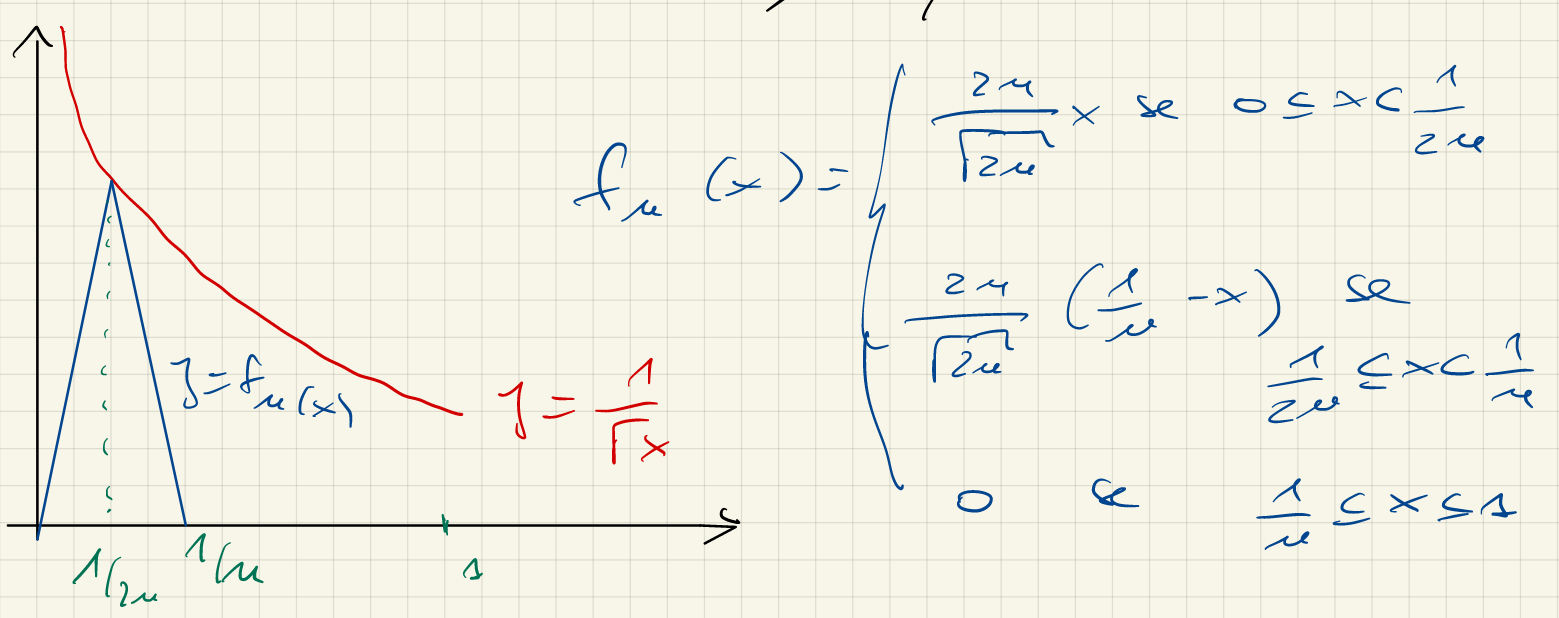
\includegraphics[width=0.7\textwidth]{Screenshot from 2023-03-28 20-48-27}
    \end{figure}
    
    $\parallel f_n \parallel_\infty = \sqrt{2n}\rightarrow +\infty$ se $n\rightarrow +\infty$, $f_n \in K$
    \item $C^\circ ([0,1]), \{f_n\}_{n\geq 1}$ come sopra. Allora $f_n \rightarrow f=0$ per $\parallel \cdot \parallel_1$\\
    $\parallel f_n -0 \parallel_1 =\int_{0}^{1} |f(x)|dx =\frac{1}{n} \sqrt{2n}\frac{1}{2}= \frac{1}{\sqrt{2n}} \rightarrow 0$ per $n \rightarrow +\infty$\\
    Ma $\parallel f_n -0 \parallel_\infty = \sqrt{2n} \rightarrow +\infty \Rightarrow f_n \nrightarrow 0$ per $\parallel \cdot \parallel_\infty$
\end{itemize}


\paragraph{\textcolor{red}{Osservazione}}
$K \subseteq \R^n$ è limitato per $|\cdot| \Leftrightarrow$ lo è per $\parallel \cdot \parallel_\infty \Leftrightarrow$ lo è per $\parallel \cdot \parallel_1$\\
$\parallel \overline{x} \parallel_\infty \leq |\overline{x}|\leq \parallel \overline{x} \parallel_1 \leq n \parallel\overline{x} \parallel_\infty$\\
\begin{figure}[!h]
    \centering
    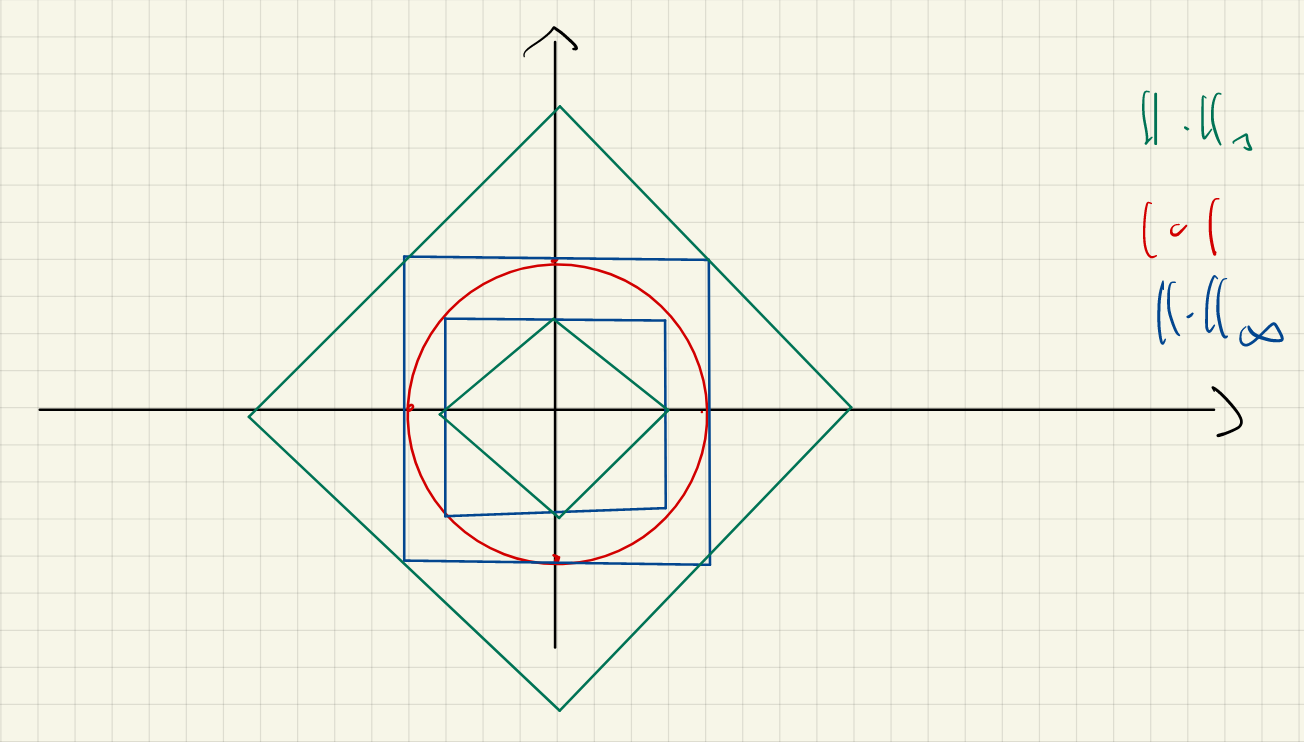
\includegraphics[width=0.7\textwidth]{Screenshot from 2023-03-28 20-55-22}
\end{figure}

\paragraph{\textcolor{red}{Osservazione}}
Introduciamo in $\R^n$ il simbolo $\infty$. Un intorno di $\infty$ è un qualunque insieme $A \subseteq \R^n$ tale che $A$ contiene il complementare di una palla di centro l'origine, cioè $\exists R>0$ tale che $\overline{x} \in A \Rightarrow \parallel \overline{x} \parallel > R$\\
\begin{figure}[!h]
    \centering
    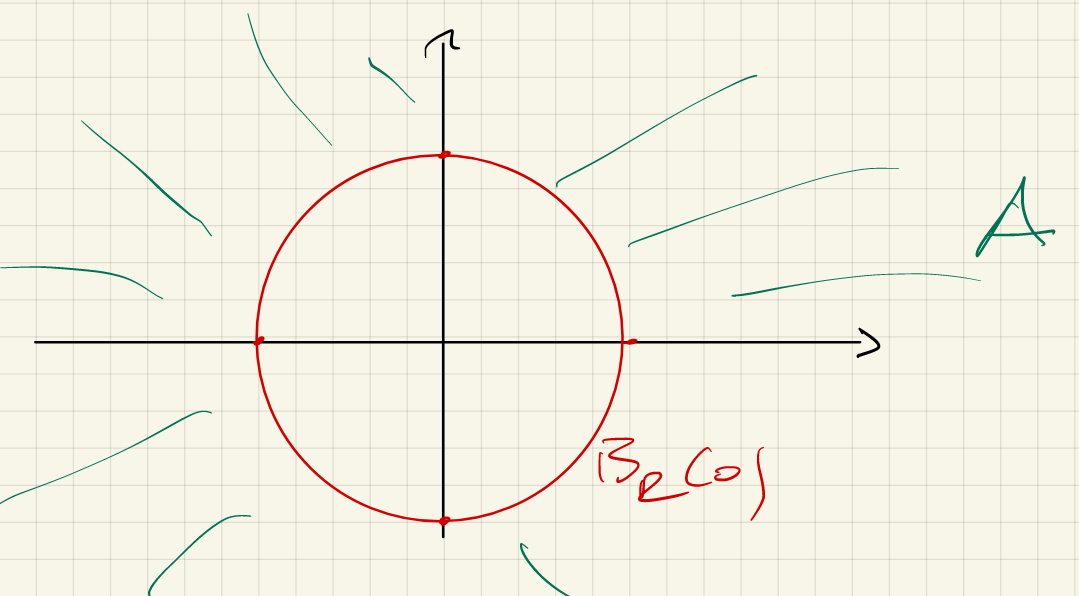
\includegraphics[width=0.5\textwidth]{Screenshot from 2023-03-28 21-04-48}
\end{figure}

Una successione $\{\overline{x_k}\}_{k\geq 1} \subseteq \R^n$ si dice divergente a $\infty$ e si scrive $\lim_{k \rightarrow \infty} \overline{x_k}=\infty$ se $\lim_{k \rightarrow \infty} |\overline{x_k}|=+\infty$ cioè se $\forall\,\, R > 0\,\, \exists\, N >0\,\,|\,\,k>N \Rightarrow |\overline{x_k}|>R$

\paragraph{\textcolor{red}{Esempio}}
$\overline{x_k}=(e^{-k},2+\frac{1}{k},\ln k) \subseteq \R^3,\,\, k \geq 1$\\
$\lim_{k}x_{k1}=\lim_{k}e^{-k}=0$\\
$\lim_{k}x_{k2}=\lim_{k}2+\frac{1}{k}=2$\\
$\lim_{k}x_{k3}=\lim_{k}\ln k=+\infty$\\
$\lim_{k}|\overline{x_k}|=\lim_{k} \sqrt{e^{-2k}+(2+\frac{1}{k})^2+(\ln k)^2} = +\infty \Rightarrow \lim_{k} \overline{x_k}=\infty$

\subsection{\textcolor{red}{Limiti di Funzione}}
\paragraph{\textcolor{red}{Definizione}}
$(X,d)$ spazio metrico, $A \subseteq X$, non vuoto. $x_0 \in X$ si dice \textcolor{red}{punto di accumulazione} per $A$ se  $\forall \epsilon >0 \,\, \exists \,\, x \in A, x \neq x_0,$ tale che $x \in B_\epsilon(x_0)$, cioè se $B_\epsilon (x_0) \cap A$ contiene punti di $A$ diversi da $x_0$. $x_0 \in A$ si dice \textcolor{red}{punto isolato} se non è di accumulazione, cioè se $\exists \epsilon >0$ tale che $B_\epsilon (x_0) \cap A =\{x_0\}$.

\paragraph{\textcolor{red}{Definizione}}
$(X,d_x),(Y,d_y)$ spazi metrici, $f:dom f \rightarrow Y$, con $domf \subseteq X, x_0 \in X $ punto di accumulazione per $domf$. Si dice che $f$ ha limite $l \in Y$ per $x \rightarrow x_0$ e si scrive
\begin{empheq}{equation*}
    \lim_{x \rightarrow x_0} f(x)=l \,\,\,\,\,\, \text{oppure} \,\,\,\,\,\, f(x) \rightarrow l \,\,\,\, \text{per} \,\,\, x \rightarrow dx_0
\end{empheq}
se per ogni intorno  $V$ di $l$  esiste un intorno $U$ di $x_0 $ tale che $ f(x) \in V$, $x \in U \cap domf, x \neq x_0$\\
In altre parole, $\lim_{x \rightarrow x_0} f(x) =l\,\,\forall\,\, \epsilon >0 \,\ \exists \,\, \delta >0 \,\,|$ se $0 < d(x,x_0) < \delta$ e $x \in domf $, allora $d_y(f(x),l)<\epsilon$\\
\textcolor{orange}{Se prendo la definizione data con $\epsilon$ e $\delta$ per $X=Y=\R$ e le distanze $d_x(x,y)=d_y(x,y)=|x-y|$, ottengo la definizione con $\epsilon$ e $\delta$ data in ambito reale.}

\paragraph{\textcolor{red}{Teorema di unicità del limite}}
$(X,d_x)$ e $(Y,d_y)$ spazi metrici, $f: domf \rightarrow Y$, $domf \subseteq X, x_0 \in X$ punto di accumulazione per $domf$.\\
Se $\lim_{x \rightarrow x_0} f(x) = l_1 \in Y$ e $\lim_{x \rightarrow x_0} f(x) = l_2 \in Y$, allora $l_1=l_2$.

\paragraph{\textcolor{red}{Proposizione}}
$(X,d)$ spazio metrico, $\overline{f}: dom\overline{f} \rightarrow \R^n,\,\, \overline{f}(x)=(f_1(x),...,f_n(x))$, $x_0 \in X$ punto di accumulazione per $dom \overline{f} \subseteq X$, allora $\lim_{x \rightarrow x_0} \overline{f}(x)=\overline{l}=(l_1,...,l_n)\in \R^n \Leftrightarrow \lim_{x \rightarrow x_0} f_j(x)=l_j \forall j=1,2,...,n$.

\paragraph{\textcolor{red}{Teorema della permanenza del segno}}
$(X,d)$ spazio metrico, $f: domf \rightarrow\R$, $domf \subseteq X, x_0 \in X$ punto di accumulazione per $domf$.\\
Se $\lim_{x \rightarrow x_0} f(x) = l >0$, allora $f(x)>0$ definitivamente per $ x \rightarrow x_0$, cioè $\exists \,\, \delta >0 \,\, |\,\, f(x)>0 \,\, \forall \,\, x \in B_\delta (x_0)\cap domf$, $x \neq x_0$. 

\paragraph{\textcolor{red}{Teorema}}
$(X,d)$ spazio metrico, $f,g: A \rightarrow\R$, $A \subseteq X, x_0 \in X$ punto di accumulazione per $A$, tali che $\lim_{} f(x) =l_f$, $\lim_{x \rightarrow x_0} g(x)=l_f$ e $f(x)\leq g(x)$ definitivamente per $x \rightarrow x_0$. \\\textcolor{orange}{$\exists \delta > 0 | f(x) \leq g(x) \forall x \in B_\delta (x_0) \cap A$, $x \neq x_0$.)}\\ Allora $l_f \leq l_g$.

\paragraph{\textcolor{red}{Teorema del Confronto}}
$(X,d)$ spazio metrico, $f,g,h : A \rightarrow \R, A \subseteq X, x_0$ punto di accumulazione per $A$, tali che $g(x) \leq f(x)\leq h(x)$ definitivamente per $x \rightarrow x_0$. Se $\lim_{x \rightarrow x_0} g(x)=\lim_{x \rightarrow x_0} h(x)=l$, allora $\lim_{x \rightarrow x_0} f(x)=l$.

\newpage
\section{\textcolor{red}{Lezione 14 \space\space 28/03/'23}}
\subsection{\textcolor{red}{Funzioni continue tra spazi metrici}}
\paragraph{\textcolor{red}{Definizione}}
$(X,d_x),(Y,d_y)$ spazi metrici, $f:domf \rightarrow Y, domf \subseteq X$, si dice \textcolor{red}{continua in $x_0 \in domf$} se vale una delle due
\begin{enumerate}
    \item $x_0$ è punto isolato per $domf$
    \item $\lim_{x \rightarrow x_0} f(x)=f(x_0)$
\end{enumerate}
In altre parole, $f$ è continua in $x_0$ se $\forall \epsilon >0\,\, \exists \,\,\delta >0$ tale che se $d_x(x,x_0)<\delta$ e $ x \in domf$, allora $d_y(f(x),f(x_0)<\epsilon$.\\
\textcolor{orange}{$x \in B_{\delta}^{x}(x_0)\cap domf \Rightarrow f(x) \in B_{\epsilon}^{y}(f(x_0))\Rightarrow x \in f^{-1}(B_{\epsilon}^{y}(f(x_0)))$}\\
\textcolor{orange}{$\forall \,\, \epsilon >0 \,\, \exists\,\, \delta >0 \,\, |\,\, B_{\delta}^{x}(x_0)\cap domf \subseteq f^{-1}(B_{\epsilon}^{y}(f(x_0)))$}\\
Una funzione $f:domf\rightarrow Y $ si dice continua se è continua in ogni punto del suo dominio.

\paragraph{\textcolor{red}{Teorema}}
$(X,d_x),(Y,d_y)$ spazi metrici, $f:X \rightarrow Y$. $f$ è continua $\Leftrightarrow f^{-1}(A)$ è aperto (in $X$) per ogni aperto $A \subseteq Y$.

\paragraph{\textcolor{red}{Dimostrazione (esercizio)}}
\begin{itemize}
    \item $\Rightarrow)$ Ipotesi: $f$ continua. Tesi: Dato $A \subseteq Y$ aperto, $f^{-1}(A)\subseteq X$ è aperto.\\
            Sia $x_0 \in f^{-1}(A)$. Dobbiamo trovare una palla centrata in $x_0$ contenuta in $f^{-1}(A)$.\\
            $f(x_0) \in A$, che è aperto, $\exists \epsilon >0$ tale che $B_{\epsilon}^{Y}(f(x_0))\subseteq A$, $\exists \delta >0 $ tale che $B_{\delta}^{x}(x_0) \Rightarrow f(x)\in B_{\epsilon}^{Y}(f(x_0))\subseteq A$.\\
            $B_{\delta}^{x}(x_0) \subseteq f^{x_0} (A)$, come si voleva.
    \item $\Leftarrow)$ Ipotesi: $f^{-1}(A)\subseteq X$ è aperto $\forall A \subseteq Y$ aperto. Tesi: $f$ è continua\\
        Fissiamo $x_0 \in X$ e $\epsilon >0$.\\
        Dobbiamo trovare $\delta >0 $ tale che $x \in B_{\delta}^{x} (x_0) \Rightarrow f(x) \in B_{\epsilon}^{y} (f(x_0))$\\
        $B_{\epsilon}^{y} (f(x_0))$ è un aperto $\Rightarrow f^{-1}(B_{\epsilon}^{y} (f(x_0)))$ è aperto e $x_0 \in f^{-1}(B_{\epsilon}^{y} (f(x_0))) \Rightarrow \exists\,\, \delta >0 $ tale che $B_{\delta}^{x}(x_0) \subseteq f^{-1}(B_{\epsilon}^{y}(f(x_0)))$ cioè, se $x \in B_{\delta}^{x}(x_0) \Rightarrow f(x) \in B_{\epsilon}^{y}(f(x_0))$ come si voleva.
\end{itemize}
\begin{flushright}
\large\Lightning
\end{flushright}

\paragraph{\textcolor{red}{Teorema}}
$(X,d)$ spazio metrico. $A \subseteq X, f,g: A \rightarrow \R, x_0 \in A$, $f$ e $g$ continue in $x_0$. Allora $f+g, f\cdot g$ e $f/g$, se $g(x_0)\neq 0$, sono continue in $x_0$.

\paragraph{\textcolor{red}{Proposizione}}
$(X,d)$ spazio metrico, $A \subseteq X, \overline{f}: A \rightarrow \R^n$\\
$\overline{f}(x)=(f_1(x),...,f_n(x))$, è continua in $x_0 \in A \Leftrightarrow$ sono continue in $x_0$ le sue componenti $f_j \forall j=1,...,n$.

\paragraph{\textcolor{red}{Esempio}}
$(X,d_x),(Y,d_y)$ spazi metrici.
\begin{enumerate}
    \item Provare che $d((x_1,y_1),(x_2,y_2))= \sqrt{(d_x(x_1,x_2))^2+(d_y(y_1,y_2))^2}$ con $(x_1, y_1),(x_2,y_2)\in X \times Y$ è una metrica in $X\times Y$.
    \item Provare che $\forall r >0$ vale\\
        $B_{\frac{r}{\sqrt{2}}}^{X}(x) \times B_{\frac{r}{\sqrt{2}}}^{Y}(y) \subseteq B_{r}^{X\times Y}((x_0,y_0))\subseteq B_{r}^{X}(x_0)\times B_{r}^{Y}(y_0)$.
        \begin{figure}[!h]
            \centering
            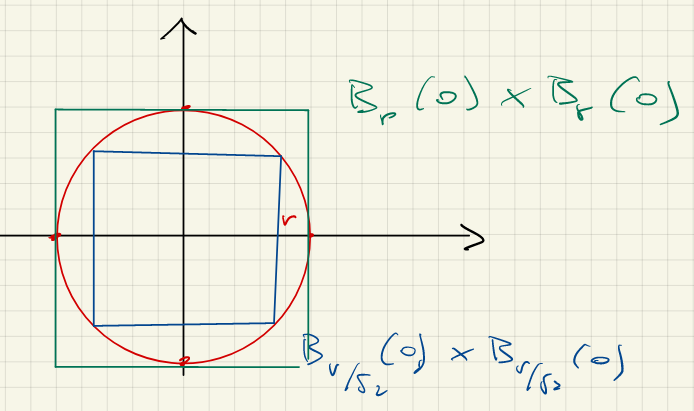
\includegraphics[width=0.5\textwidth]{Screenshot from 2023-03-28 21-59-39.png}
        \end{figure}
    \item Sia ora $Y=\R$ con la metrica usuale che deriva dal valore assoluto.\\
        $f:X \rightarrow \R$\\
        $A=\{  (x,y)\in X\times \R |y>f(x) \}$\\
        $C=\{  (x,y)\in X\times\R |y \geq f(x) \}$\\
        Provare che se $f $ è continua, allora $A$ è aperto e $C$ è chiuso in $X \times \R$ con la metrica $d$.
    \item Provare che, in generale, il viceversa non è vero, cioè $A$ può essere aperto con $f$ discontinua e $C$ chiuso con $f$ discontinua.
\end{enumerate}
\begin{enumerate}
    \item Per casa
    \item Facciamo vedere che se $(x,y)\in B_{\frac{r}{\sqrt{2}}}^{X}(x_0) \times B_{\frac{r}{\sqrt{2}}}^{Y}(y_0)$, allora $(x,y) \in B_{r}^{X\times Y}((x_0,y_0))$\\
    $d_x(x,x_0)< \frac{r}{\sqrt{2}}$ e $d_y(y,y_0)< \frac{r}{\sqrt{2}}$\\
    $\Rightarrow d((x,y),(x_0,y_0))<r$, $d((x,y),(x_0,y_0))=\sqrt{(d_x(x_1,x_2))^2+(d_y(y_1,y_2))^2} <$\\
    $< \sqrt{\left( \frac{r}{\sqrt{2}} \right)^2+\left( \frac{r}{\sqrt{2}} \right)^2} = \sqrt{r^2} =r$\\
    Facciamo vedere che, se $(x,y)\in B_{r}^{X\times Y}((x_0,y_0))$, allora $(x,y)\in B_{r}^{X}(x_0) \times B_{r}^{Y}(y_0)$, cioè che, se $d((x,y),(x_0,y_0))<r$, allora $d_x(x,x_0)<r$ e $d_y(y,y_0)<r$\\
    $d_x(x,x_0)= \sqrt{(d_x(x,x_0))^2}\leq \sqrt{(d_x(x,x_0))^2+(d_y(y,y_0))^2}= d((x,y),(x_0,y_0))<r$
    \item Introduciamo la funzione $\phi: X\times\R \rightarrow \R, (x,y)\mapsto y-f(x)$ \textcolor{orange}{(c'è la metrica $d$)}\\
    $A= \{ (x,y)\in X\times\R | \phi(x,y)>0\} = \phi^{-1}(]0,+\infty[)$\\
    $C = \{ (x,y)\in X\times\R | \phi(x,y)\geq 0\} = \phi^{-1}(]0,+\infty[)$\\
    $\phi^{-1}(B^c)=(\phi^{-1}(B))^c$\\
    $x \in \phi^{-1}(B^c) \Leftrightarrow \phi(x)\in B^c \Leftrightarrow \phi(x)\notin B \Leftrightarrow x \notin \phi^{-1}(B) \Leftrightarrow x \in (\phi^{-1}(B))^c$\\
    Se $B$ è chiuso e $\phi$ è continua, $\phi^{-1} (B) = \phi^{-1}((B^c)^c)=(\phi^{-1}(B^c))^c$ è chiuso, cioè l'antimmagine di un chiuso tramite una funzione continua è un insieme chiuso.\\
    Poichè $B= [0,+\infty[$ è chiuso e $C= \phi^{-1}(B)$, se $\phi$ è continua, $C$ è chiuso.\\
    Tutto l'esercizio si riduce a dimostrare che $\phi$ è continua.\\
    $\phi_1: X \times \R \rightarrow \R, (x,y)\mapsto y$ e $\phi_2: X\times\R \rightarrow \R, (x,y)\mapsto f(x)$\\
    $\phi(x,y)=\phi_1(x,y)-\phi_2(x,y)$\\
    Se dimostro che $\phi_1$ e $\phi_2$ sono continue, allora $\phi$ è continua perchè differenza di funzioni continue.\\
    Dimostriamo la continuità di $\phi_1$\\
    $(x_0,y_0) \in X \times \R$ e fissiamo $\epsilon >0$\\
    Dobbiamo dimostrare che $\exists \delta >0 $ tale che se $d((x,y),(x_0,y_0))<\delta$, allora $|y-y_0|<\epsilon$\\
    Sia $U = X \times  ]y_0-\epsilon,y_0+\epsilon[$\\
    Se $(x,y)\in U \Rightarrow |\phi_1(x,y)-\phi_1(x_0,y_0)|=|y-y_0|<0$\\
    $U$ è un intorno di $(x_0,y_0)$, cioè $\exists \delta >0 | B_{\delta}^{X \times \R}((x_0,y_0))\subseteq U$\\
    $B_{\delta}^{X\times \R}((x_0.y_0))\subseteq B_{\delta}^{X}(x_0) \times B_{\delta}^{\R}(y_0)\subseteq X\times ]y_0-\epsilon,y_0+\epsilon[$\\
    Continuità di $\phi_2$ in $(x_0,y_0)$\\
    $\forall \epsilon >0$ devo trovare $\delta >0$ tale che se $d((x,y),(x_0,y_0))< \delta \Rightarrow |\phi_2(x,y)-\phi_2(x_0,y_0)|=|f(x)-f(x_0)|<\epsilon$\\
    Poichè $f$ è continua, $\exists \delta >0$ tale che $ x \in B_{\delta}^{X} (x_0) \Rightarrow |f(x)-f(x_0)|<\epsilon$\\
    L'insieme $B_{\delta}^{X}(x_0) \times \R$ è un intorno di $(x_0,y_0)$ e $\forall (x,y) \in B_{\delta}^{X}(x_0) \times \R$ si ha $|\phi_2(x,y)-\phi(x_0,y_0)|=|f(x)-f(x_0)|<\epsilon$
    \item $X=Y=\R$ con la distanza data dal valore assoluto\\
    $f(x)=\chi_{[0,+\infty[}(x) \begin{cases}
         &1 \,\,\,\,\,\text{se}\,\,\,\,\, x \geq 0\\
        &0\,\,\,\,\, \text{se}\,\,\,\,\, x < 0
    \end{cases}$ \\
    \textcolor{orange}{(funzione caratteristica di $[0,+\infty[$ o funzione di Heaviside)}\\
    \begin{figure}[!h]
        \centering
        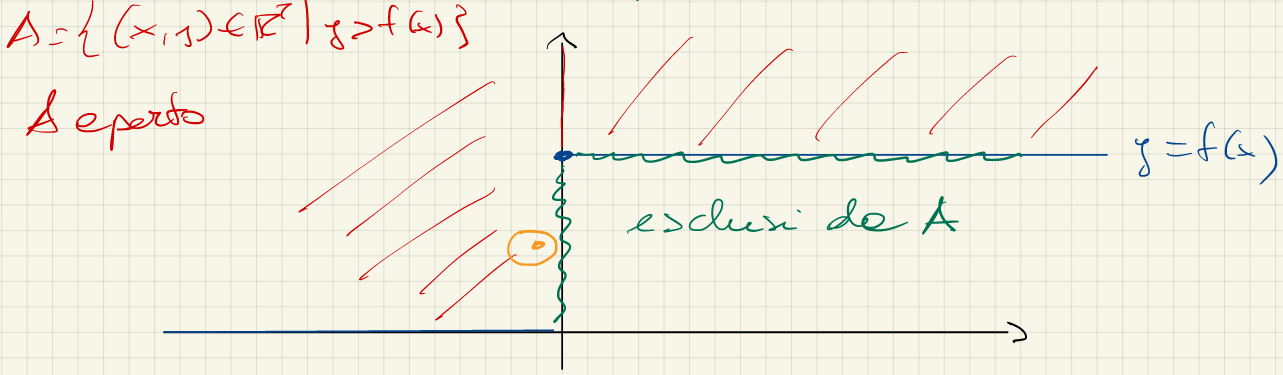
\includegraphics[width=0.7\textwidth]{Screenshot from 2023-03-28 22-16-16.png}
    \end{figure}
    
    $f(x)=\chi_{]0,+\infty[}=\begin{cases}
        &1 \,\,\,\,\,\text{se}\,\,\,\,\, x > 0\\
        &0\,\,\,\,\, \text{se}\,\,\,\,\, x \leq 0
    \end{cases}$
    \begin{figure}[!h]
        \centering
        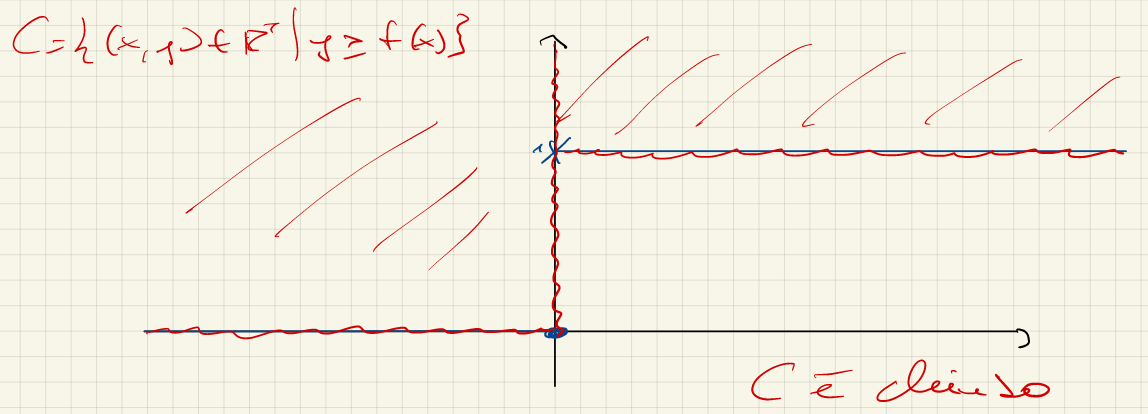
\includegraphics[width=0.7\textwidth]{Screenshot from 2023-03-28 22-17-48.png}
    \end{figure}
\end{enumerate}

\subsection{\textcolor{red}{Successioni di funzioni}}
\paragraph{\textcolor{red}{Definizione}}
$(X,d)$ spazio metrico.\\
Una successione di funzioni da $X$ in $\R$ è una funzione che ad ogni numero naturale $k$ associa una ed una sola funzione $f_k:X\rightarrow \R$. 

\paragraph{\textcolor{red}{Definizione}}
Sia $\{ f_k \}_{k\in\N}, f_k:X \rightarrow \R$, successione di funzioni. Si dice che la successione \textcolor{red}{converge puntualmente} in $D \subseteq X$ se $\{f_k(x)\}_{k\in\N}$ converge $\forall x \in D$, cioè se $\forall x \in D$ esiste finito
\begin{equation*}
    \lim_{k\rightarrow +\infty} f_k(x)=f(x),
\end{equation*}
limite puntuale della successione $f : D \rightarrow \R$. L'insieme degli $x \in X$ dove $\{f_k \}_{k \in \N}$ converge puntualmente si dice \textcolor{red}{insieme di convergenza puntuale} della successione.

\paragraph{\textcolor{red}{Esempio}}
$f_k:\R \rightarrow \R, f_k(x)=x^k$\\
$\lim_{k\rightarrow +\infty} f_k(x)=\lim_{k\rightarrow +\infty} x^k =\begin{cases}
    & 0\,\,\,\,\, \text{se} \,\,\,\,\, |x|<1 \\
    & 1 \,\,\,\,\, \text{se}\,\,\,\,\, x=1 \\
    & \nexists  \,\,\,\,\, \text{se}\,\,\,\,\, x \leq -1\\
    & +\infty  \,\,\,\,\, \text{se}\,\,\,\,\, x >1
\end{cases}$\\
Insieme di convergenza puntuale: $D=]-1,1]$\\
Limite puntuale $f:D \rightarrow \R, f(x)=\begin{cases}
    &0 \,\,\,\,\, \text{se}\,\,\,\,\, |x|<1\\
    &1  \,\,\,\,\, \text{se}\,\,\,\,\, x=1
\end{cases}$ 

\paragraph{\textcolor{red}{Definizione}}
$f_k:X \rightarrow \R, k \in \N$, successione di funzione. Si dice che $\{ f_k\}_{k\in\N}$ \textcolor{red}{converge uniformemente} in $D \subseteq X$ ad una funzione $f: D\rightarrow \R$ se 
\begin{equation*}
    \lim_{k\rightarrow+\infty}\sup_{x\in D}|f_k(x)-f(x)|=0
\end{equation*}
e si scrive $f_k \rightrightarrows f$ in $D$\\
\textcolor{orange}{$\forall \epsilon >0 \exists N | k >N$\\ 
$\sup_{x\in D}|f_k(x)-f(x)| <\epsilon$, e quindi, in particolare $|f_k(x)-f(x)|<\epsilon \forall x \in D$ cioè $f(x)-\epsilon <f-k(x)<f(x)+\epsilon \forall x \in D$}\\
\begin{figure}[!h]
    \centering
    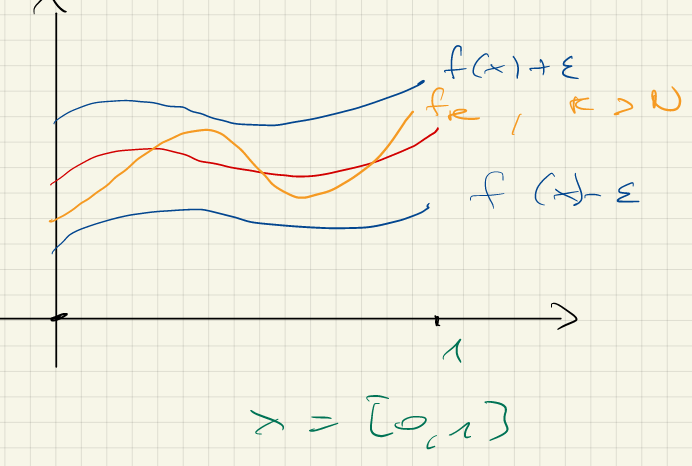
\includegraphics[width=0.5\textwidth]{Screenshot from 2023-03-28 22-27-28.png}
\end{figure}

$(X,d)$ spazio metrico\\
$B(x)=\{f:X \rightarrow \R | f$ è limitata$\}$ \textcolor{orange}{$\exists M >0 | |f(x)| \leq M \forall x \in X$}\\
$f\in B(x)$, $\parallel f \parallel_\infty =\sup_{x\in X}|f(x)|$, norma infinito di $f$\\
$f_k \rightrightarrows f$ in $X$ se $\parallel f_k - f \parallel_\infty \rightarrow 0$ per $k \rightarrow +\infty$\\
cioè la convergenza uniforme è la convergenza per $\parallel \cdot \parallel_\infty$.

\paragraph{\textcolor{red}{Proposizione}}
Se $f_k \rightrightarrows f$ in $ D $, allora $\{ f_k \}_{k \in \N}$ converge puntualmente ad $f$ in $D$.

\paragraph{\textcolor{red}{Dimostrazione}}
Se $x \in D$, $0 \leq |f_k(x) -f(x)| \leq \sup_{y\in D}|f_k(y)-f(y)| \Rightarrow |f_k(x)-f(x)|\rightarrow 0$ per $ k \rightarrow +\infty$ cioè $f(x)=\lim_{k \rightarrow +\infty f_k (x)} \forall x \in D$.
\begin{flushright}
\large\Lightning
\end{flushright}

\newpage
\section{\textcolor{red}{Lezione 15 \space\space 30/03/'23}}
\paragraph{\textcolor{red}{Esempio}}
$f_k(x)=x^k$, $x \in \R$\\
Insieme di convergenza puntuale è $D=]-1,1]$\\
Limite puntuale $f:D \rightarrow \R$\\
$f (x)= \begin{cases}
    & 0 \,\,\,\,\, \text{se} \,\,\,\,\, -1 < x<1\\
    & 1 \,\,\,\,\, \text{se} \,\,\,\,\, x=1
\end{cases}$\\
$f_k \rightrightarrows f$ in $D$?\\

\textcolor{orange}{$g_k(x)= \frac{e^{-x^2}}{k}$, $x \geq 1, x \in \R$\\
$\lim_{k \rightarrow +\infty} g_k(x)=0\,\, \forall x$\\
$\{g(x)\}_{k \geq 1}$ converge puntualmente alla funzione nulla $g(x)=0 \,\, \forall x\in\R$ in $\R$\\
$\sup_{x \in \R} |g_k(x)-g(x)|=\sup_{x\in\R} \frac{e^{-x^2}}{K}=\frac{1}{k} \rightarrow 0$\\
$g_k \rightrightarrows g$ in $\R$}\\

\textcolor{orange}{$\phi_k(x)= \frac{x^2}{k}$, $k \geq 1, x \in \R$\\
$\lim_{k \rightarrow +\infty} \phi_k(x)=0=\phi(x) \,\, \forall x \in \R$\\
Insieme di convergenza puntuale è $\R$ e il limite puntuale è la funzione nulla\\
$\sup_{x\in\R}|\phi_k(x)-\phi(x)|=\sup_{x\in\R} \frac{x^2}{k}=+\infty$\\
$\phi_k \nrightrightarrows \phi$ in $\R$\\
Fissato $M>0$, ho convergenza uniforme in $[-M,M]$?\\
$\sup_{x \in [-M,M]}|\phi_k(x)-\phi(x)|=\sup_{x\in [-M,M]} \frac{x^2}{k}=\frac{M^2}{k} \rightarrow 0$ per $k \rightarrow + \infty$\\
$\phi_k \rightrightarrows \phi$ in $[-M,M] \,\, \forall M >0$} \textcolor{red}{ma non in $\R$.}\\

Torniamo a $f_k =x^k$\\
$\sup_{x \in ]-1,1]}|f_k(x)-f(x)| \geq \sup_{x \in ]-1,1[}|f_k(x)-f(x)|= \sup_{x \in ]-1,1[}|x^k|=1\,\,\, \forall k$\\
$f_k \nrightrightarrows f$ in $]-1,1]$\\
Sia $0<\epsilon < 1$ e studiamo la convergenza uniforme in $[-1+\epsilon,1-\epsilon]$\\
$\sup_{x \in [-1+\epsilon,1-\epsilon]}|f_k(x)-f(x)|=\sup_{x \in [-1+\epsilon,1-\epsilon]}|f_k(x)|=\sup_{x \in [-1+\epsilon,1-\epsilon]}|x^k|=(1-\epsilon)^k \rightarrow 0$ per $k \rightarrow +\infty$ perchè $0<1-\epsilon <1 \Rightarrow f_k \rightrightarrows f$ in $ [-1+\epsilon, 1-\epsilon] \,\, \forall \epsilon>0$ \textcolor{red}{ma non in ]-1,1]!}

\paragraph{\textcolor{red}{Esempio}}
$f_k(x)=\frac{kx}{1+k|x|}, \,\, k \geq 0, x \in \R$\\

Convergenza puntuale
\begin{equation*}
    \lim_{k\rightarrow +\infty} f_k(x) = \begin{cases}
    & 1 \,\,\,\,\, \text{se}\,\,\, x >0 \\
    & 0 \,\,\,\,\, \text{se}\,\,\, x=0 \\
    & -1  \,\,\,\,\, \text{se}\,\,\, x<0
\end{cases}
\end{equation*}
L'insieme di convergenza puntuale è $\R$ e il limite puntuale è la funzione segno
\begin{equation*}
    sgn(x)= \begin{cases}
    & 1  \,\,\,\,\, \text{se}\,\,\, x>0 \\
    & 0  \,\,\,\,\, \text{se}\,\,\, x=0\\
    & -1  \,\,\,\,\, \text{se}\,\,\, x<0
\end{cases}
\end{equation*}
$\sup_{x\in\R}|f_k(x)-sgn(x)|\geq \sup_{x>0} |f_k(x)-sgn(x)|=\sup_{x>0}|\frac{kx}{1+kx}-1|=\sup_{x>0}|\frac{1}{1+kx}|=1$\\
$f_k \nrightrightarrows sgn$ in $\R$\\
Fissiamo $\epsilon >0$ e studiamo la convergenza uniforme in $]-\infty-\epsilon]\cup[\epsilon,+\infty[$\\
$\sup_{|x|\geq \epsilon} |f_k(x)-sgn(x)|=\sup_{x \geq \epsilon} |f_k(x)-sgn(x)|= \sup_{x \geq \epsilon} |\frac{1}{1+kx}|= \frac{1}{1+k\epsilon}\rightarrow 0$ per $k \rightarrow +\infty$\\
$f_k \rightrightarrows sgn$ in $]-\infty,-\epsilon]\cup[\epsilon,+\infty[\,\,\, \forall \epsilon >0$, \textcolor{red}{ma non in $\R\backslash \{0\}$}\\
$\sup_{x\in\R\backslash \{0\}}|f_k(x)-sgn(x)|=\sup_{x >0}|f_k(x)-sgn(x)|=1\,\, \forall k$.

\paragraph{\textcolor{red}{Teorema}}
$(X,d)$ spazio metrico, $f_k:X \rightarrow \R$, $\{f_k\}_{k \in \N}$ successione di funzioni tale che $f_k \rightrightarrows f$ in $D$. Se $f_k$ è continua in $x_0 \in X \,\, \forall\,\, k \in \N$, allora $f$ è continua in $x_0$. In particolare, se $f_k \in C^\circ(X)\,\, \forall \,\, k \in \N$, allora $f \in C^\circ(X)$ \textcolor{orange}{(il limite uniforme di funzioni continue è continuo)}.

\paragraph{\textcolor{red}{Osservazione}}
$f_k(x)=\frac{kx}{1+k|x|}$ non può convergere uniformemente a $sgn$ in $\R$ perchè $f_k \in C^\circ (\R)\,\, \forall \,\, k$, ma $sgn$ ha un punto di salto in $x=0$.

\paragraph{\textcolor{red}{Dimostrazione}}
$x_0 \in X$. Fissiamo $\epsilon >0$.\\
Dobbiamo dimostrare che $\exists \delta >0\,\, |\,\, d(x,x_0) <\delta \Rightarrow |f(x)-f(x_0)|<\epsilon$
\begin{itemize}
    \item $f_k$ è continua in $x_0 \,\, \forall \,\, k$
    \item $f_k \rightrightarrows f$ in $X$
\end{itemize}
$f_k \rightrightarrows f$ in $X \Rightarrow \exists\,\, N >0 \,\,|\,\, k >N \Rightarrow |f_k (x)-f(x)|< \frac{\epsilon}{3} \,\, \forall \,\, x \in X$ perchè $\sup_{x\in X}|f_k(x)-f(x)|<\frac{\epsilon}{3}$.\\
Fissiamo $\overline{k}>N$, cosicchè $|f_{\overline{k}}(x) -f(x)|<\frac{\epsilon}{3} \,\,\forall \,\, x \in X$ e sia $\delta >0 \,\,|\,\, d(x,x_0) <\delta$\\$\Rightarrow |f_{\overline{k}}(x) -f_{\overline{k}}(x_0)| <\frac{\epsilon}{3}$ ($\delta$ esiste perchè $f_{\overline{k}}$ è continua in $x_0$).\\
$|f(x)-f(x_0)| =|(f(x)-f_{\overline{k}}(x))+(f_{\overline{k}}(x)-f_{\overline{k}}(x_0))+(f_{\overline{k}}(x_0)-f(x_0))|\leq |f(x)-f_{\overline{k}}(x)|+|f_{\overline{k}}(x)-f_{\overline{k}}(x_0)|+|f_{\overline{k}}(x_0)-f(x_0)| < \frac{\epsilon}{3}+\frac{\epsilon}{3}+\frac{\epsilon}{3}=\epsilon$ a patto che $d(x,x_0)< \delta$
\begin{flushright}
\large\Lightning
\end{flushright}

\newpage
\section{\textcolor{red}{Lezione 16 \space\space 03/04/'23}}
\paragraph{\textcolor{red}{Osservazione}}
Tutto quello che abbiamo detto e che diremo  per successioni di funzioni a valori in $\R$ vale per successioni di funzioni a valori in $\C$.

\paragraph{\textcolor{red}{Esempio}}
$\phi: [0,1]\rightarrow \R^{\geq 0}$ continua com $C=\{ f \in C^\circ ([0,1]) \,\,|\,\,|f(x)|\leq \phi(x) \forall x \in [0,1]\}$.\\
Dotato $C^\circ([0,1])$ con la norma $\parallel\cdot \parallel_\infty$, provare che $C$ è chiuso e trovare $\partial C$.
\begin{itemize}
    \item $C$ è chiuso $\Leftrightarrow$ presa $\{f_k\}_{k \in \N} \subseteq C$, convergente per $\parallel \cdot \parallel_\infty$ a $f:[0,1]\rightarrow \R$, si ha che $f \in C$.\\
    $\{f_k\}_{k\in\N} \subseteq C,\,\,\, f_k \rightrightarrows f \Rightarrow f \in C^\circ([0,1])$ perchè limite uniforme di una successione di funzioni continue. Affinchè $f \in C$, deve essere $|f(x)|\leq \phi(x) \forall x \in [0,1]$\\
    Sappiamo che $\forall x \in [0,1]\,\,\,\, |f_k(x)|\leq \phi(x) \forall k \in \N$ perchè $f_k \in C \forall k \in \N$\\
    $f_k \rightrightarrows f$ in $[0,1]\Rightarrow f_k(x) \rightarrow f(x) \forall x \in [0,1] $ perchè la convergenza uniforme implica quella puntuale $\Rightarrow |f_k(x)|\rightarrow|f(x)|\forall x \in [0,1]$.\\
    $|f_k(x)|\leq \phi(x) \,\,\, \forall x \in [0,1] \Rightarrow |f(x)|\leq \phi(x) \,\,\, \forall x \in [0,1] \Rightarrow f \in C \Rightarrow C$ è chiuso.
    \item Troviamo $\partial C$.\\
    $C=\{ f \in C^\circ ([0,1])\,\, |\,\,|f(x)|\leq \phi(x) \forall x \in [0,1]\}=\{f \in C^\circ ([0,1])\,\, |\,\, -\phi(x) \leq f(x) \leq \phi(x) \forall x \in [0,1] \}$\\
    IMMAGINE\\
    $f_0\in \partial C \Leftrightarrow \forall \epsilon > 0, B_\epsilon(f_0)\cap C \neq \emptyset$ e $B_\epsilon (f_0)\cap C^c \neq \emptyset$.\\
    Congettura: $\partial C =\{f\in C^\circ([0,1])\,\, |\,\, \exists x_0\in [0,1]\,\,|\,\, |f(x_0)|=\phi(x_0) \}$.\\
    Sia $f\in \partial C$ e proviamo che $\exists x_0 \in [0,1]\,\, |\,\, |f(x_0)|=\phi(x_0)$\\
    $f \in \partial C \Rightarrow f \in C$ perchè $C$ è chiuso $\Rightarrow |f(x)|\leq \phi(x) \,\, \forall x \in [0,1]$.\\
    Per assurdo, assumiamo che $|f(x)|<\phi(x)  \,\, \forall x \in [0,1]$.\\
    E' vero o falso che $\inf_{x \in [0,1]}( \phi(x) -|f(x)| )>0$?\\
    IMMAGINE\\
    $[0,1]$ è compatto quindi $\phi - |f|$ è continua $\Rightarrow \inf_{x \in [0,1]} [\phi(x)-|f(x)|]=\min_{x \in [0,1]} [\phi(x)- |f(x)|]= \phi(x_0)-|f(x_0)>0 =r \,\,\, \exists x_0 \in [0,1]$\\
    $\Rightarrow B_{\frac{r}{2}}(f) \leq C$ perchè, fissata $g \in B_{\frac{r}{2}}(f)$ si ha \\
    $|g(x)|\leq |g(x)-f(x)+f(x)|\leq |g(x)-f(x)|+|f(x)|<\frac{r}{2} +|f(x)|$ \textcolor{orange}{perchè $\parallel\phi-f\parallel_\infty < \frac{r}{2}$} $\leq \frac{r}{2}+\phi(x)-r =\phi(x)-\frac{r}{2} \leq \phi(x)\,\,\, \forall x \in [0,1]$\\
    $\Rightarrow g \in C \Rightarrow B_{\frac{r}{2}}(f) \cap C^c=\emptyset\Rightarrow f \notin \partial C$, assurdo.\\
    Adesso proviamo che, se $f\in C$ è tale che $\exists x_0\in [0,1]| |f(x_0)| =\phi(x_0)$, allora $f \in \partial C$, cioè $\forall \epsilon >0$, $B_\epsilon(f) \cap C \neq \emptyset$ e $B_\epsilon(f) \cap C^c \neq \emptyset$.\\
    Sicuramente $f\in B_\epsilon (f) \cap C$, che così è diverso da $\emptyset$.\\
    Basta verificare che, $\forall \epsilon >0$, $B_\epsilon (f) \cap C^c \neq \emptyset$\\
    $|f(x_0|=\phi(x_0)$. Per fissare le idee assumiamo che $f(x_0)\geq 0$\\
    $f(x_0) = |f(x_0)|= \phi(x_0)$\\
    IMMAGINE\\
    $\epsilon >0$, $f+\frac{\epsilon}{2}=g$, $ |g(x_0)|= f(x_0)+\frac{\epsilon}{2}>\phi(x_0)$\\
    $g \notin C$ e $\parallel g-f \parallel_\infty = \frac{\epsilon}{2}<\epsilon$\\
    $g \in B_\epsilon (f) \Rightarrow B_\epsilon (f) \cap C^c \neq \emptyset$, come si voleva.
    
\end{itemize}

\paragraph{\textcolor{red}{Esempio}}
Data la successione di funzioni  \\
\begin{equation*}
    f_k: \R \backslash \{0\}\rightarrow \R,\,\, k \geq 1
\end{equation*}
definita da\\
\begin{equation*}
    f_k(x)= \frac{\ln x^{2k}}{(1+x)^{2k}}
\end{equation*}
trovare gli insiemi di convergenza puntuale e uniforme.
\begin{equation*}
    \lim_{k \rightarrow +\infty}f_k(x)= \lim_{k \rightarrow +\infty}2k\frac{\ln |x|}{(1+x)^{2k}}=\begin{cases}
         +\infty \,\,\,\,& \text{se}\,\,\, |1+x|\leq 1 \,\,\,\,\, \text{e}\,\,\, |x|>1 \\
         -\infty \,\,\,\,& \text{se}\,\,\, |1+x|\leq 1 \,\,\,\,\, \text{e}\,\,\, |x|<1 \\
         0 \,\,\,\,& \text{se}\,\,\, |1+x|\geq 1
    \end{cases}
    =\begin{cases}
         +\infty \,\,\,\, &\text{se}\,\,\, -2 \leq x <- 1 \\
         -\infty \,\,\,\, &\text{se}\,\,\, -1 < x <0 \\
         0 \,\,\,\, &\text{se}\,\,\, x< -2 \,\,\, \text{o}\,\,\, x >0
    \end{cases}
\end{equation*}
L'insieme di convergenza puntuale è $D=]-\infty,-2[\cup ]0,+\infty[$ e il limite puntuale è la funzione $f(x) = 0\,\,\, \forall x \in D$.\\
Studiamo la convergenza uniforme in $D$ e studiamo separatamente gli intervalli $]-\infty,-2[$ e $]0,+\infty[$.\\
Valutiamo 
\begin{equation*}
    \sup_{x >0} |f_k(x)-f(x)|= \sup_{x >0}|f_k (x)|=\sup_{x>0}2k \frac{|\ln |x||}{(1+x)^{2k}}\geq \lim_{x \rightarrow 0^+} \frac{2k |\ln|x||}{(1+x)^{2k}}=+\infty
\end{equation*}
$f_k \nrightrightarrows f$ in $]0,+\infty[$.\\
Vediamo cosa succede in $]-\infty,-2[$
\begin{equation*}
    \sup_{x < -2}|f_k(x) -f(x)|= \sup_{x<-2} |f_k(x)|= \sup_{x <-2}2k \frac{|\ln|x||}{|1+x|^{2k}}\geq\lim_{x \rightarrow -2^-} \frac{2k|\ln |x|}{|1+x|^{2k}}= 2k\ln 2 \xrightarrow{k \rightarrow +\infty} +\infty 
\end{equation*}
$f_k \nrightrightarrows f$ in $]-\infty,-2[$.\\
Proviamo a studiare la convergenza uniforme in sottointervalli di $]0,+\infty[$ e $]-\infty,-2[$.\\
Concentriamoci su $]0,+\infty[$ e studiamo l'andamento di $f_k$ in questo intervallo \\
$f_k(x) = 2k \frac{\ln |x|}{(1+x)^{2k}},\,\,\, x >0$\\
$\lim_{x \rightarrow 0^+} f_k(x) = -\infty$\\
$\lim_{x \rightarrow +\infty} f_k(x) = 0$\\
\begin{equation*}
    f_k' (x) = 2k \frac{1+x(1-2k \ln |x|)}{x(1+x)^{2k+1}}
\end{equation*}
\begin{equation*}
    f_k' (x) \geq 0 \Leftrightarrow 1+x(1-2k \ln |x|) \geq 0,\,\,\,\, x >0
\end{equation*}
se $x \in ]0,1]$, $-\ln x \geq 0 \Rightarrow 1+x(1-2k\ln x)\geq 0$\\
$\lim_{x \rightarrow +\infty} [1+x(1-2k\ln x)]= -\infty \Rightarrow 1+x(1-2k\ln x)<0$ defintivamente per $ x \rightarrow+\infty$\\$f_k' (x) >0\,\, \forall x \in ]0,1]$ e $f_k' (x) <0$ definitivamente per $x \rightarrow +\infty$.\\
IMMAGINE\\
Devo provare a vedere più in dettaglio il segno di $f_k' $, cioè di $1+x(1-2k \ln x)$, per $x \geq 1$\\
$\phi'(x)=1-2k\ln x -2k = 1-2k(1+\ln x)< 0 \,\, \forall x >1$\\
IMMAGINE\\
$\exists ! \alpha_k >1\,\, |\,\, \phi(\alpha_k)=0 $\\
IMMAGINE\\
$\exists ! \alpha_k >1 \,\, |\,\, f_k' (\alpha_k)=0$\\
IMMAGINE\\
$\sup_{x \geq a}|f_k (x)|= \max\{|f_k(a)|,|f_k(\alpha_k)|\}\leq |f_k(a)|+|f_k(\alpha_k)|= 2k \frac{|\ln a|}{(1+a)^{2k}}+|f_k(\alpha_k)|$\\
$f_k' (\alpha_k)=0$, $ 1+\alpha_k (1-2k \ln \alpha_k)=0$\\
$1+\alpha_k - 2 k \alpha_k \ln \alpha_k=0$\\
$\ln\alpha_k= \frac{1+\alpha_k}{2k\alpha_k}$\\
$f_k (x)= 2k \frac{\ln x}{ (1+x)^{2k}},\,\,\, x >0$\\
$f_k(\alpha_k) = 2k\frac{\ln \alpha_k}{(1+\alpha_k)^{2k}}= 2k \frac{1+\alpha_k}{2k\alpha_k}\cdot \frac{1}{(1+\alpha_k)^{2k}}= \frac{1}{\alpha_k(1+\alpha_k)^{2k-1}}\leq \frac{1}{2^{2k-1}}\xrightarrow{k \rightarrow +\infty} 0 $.\\
$\sup_{x \geq a}|f_k(x)|\leq |f_k(a)|+|f_k(\alpha_k)|\xrightarrow{k \rightarrow +\infty} 0 \Rightarrow f_k \rightrightarrows f $ in $[a,+\infty[ \forall a >0$.\\
Studiamo $f_k$ in $]-\infty,-2[$.\\
$\lim_{x \rightarrow-2^-} f_k(x) = 2k\ln 2$\\
$\lim_{x \rightarrow-\infty}f_k(x) = 0 $\\
$f_k' (x) = 2k \frac{1+x(1-2k\ln|x|)}{x(1+x)^{2k+1}}$\\
Se $x <-2 $, $x(1+x)>0 \Rightarrow x(1+x)^{2k+1}>0$.\\
Se $x <-2$, $f_k'(x) \geq 0 \Leftrightarrow 1+x(1-2k\ln|x|)\geq 0$\\
$x <0$ e $1-2k\ln |x| \leq 1-2k\ln 2 <0\,\,\ \forall \alpha \geq 1$ $\Rightarrow x(1-2k\ln|x|)\geq 0 \,\, \forall x <-2$\\
$\Rightarrow f_k'(x) >0 \,\, \forall x \in ]-\infty,-2[$ $\Rightarrow f_k$ è crescente in $]-\infty,-2[$ \\
IMMAGINE\\
Fissato $b < -2$\\
$\sup_{x \leq b} |f_k(x)| = f_k(b)= 2k \frac{\ln |b|}{(1+b)^{2k}}\xrightarrow{k \rightarrow+\infty} 0$\\
$\Rightarrow f_k \rightrightarrows f$ in $]-\infty, b]\,\, \forall b < -2$.\\
$\Rightarrow f_k \rightrightarrows f$ in $]-\infty,b]\cup [a, +\infty[\,\, \forall b < -2$ e $\forall a >0$
 
\paragraph{\textcolor{red}{Osservazione}}
$(X,d)$ spazio metrico, $\{f_k\}_{k\in \N}\leq C^\circ(X)$ tale che $f_k \rightrightarrows f \in C^\circ (X)$ in $D \subseteq X$. Allora $f_k \rightrightarrows f$ in $\overline{D}$.\\
\textcolor{orange}{Riprendendo l'esercizio precedente, se $f_k \rightrightarrows f$, funzione nulla, in $]-\infty-2[$, allora dovrebbe esserci convergenza uniforme anche in $]-\infty,-2[=]-\infty,-2]$. Ma $f_k(-2)\rightarrow+\infty$, e quindi non c'è neanche convergenza puntuale.}\\
Sia $x \in \overline{D}\Rightarrow\exists \{ x_j\}_{j\geq 1} \subseteq D |x_j\rightarrow x$ per la metrica $d$\\
$|f_k(x)-f(x)|=\lim_{j}|f_k(x_j)-f(x_j)|\leq \sup_{y\in D}|f_(y)-f(y)|\,\, \forall x \in \overline{D}$\\
$\Rightarrow \sup_{x \in \overline{D}}|f_k(x)-f(x)|\leq \sup_{y \in D}|f_k(y)-f(y)| \xrightarrow{k \rightarrow+\infty} 0$ perchè $f_k \rightrightarrows f$ in $D$ \\
$\Rightarrow f_k \rightrightarrows f$ in $\overline{D}$.

\newpage
\section{\textcolor{red}{Lezione 17 \space\space 04/04/'23}}
\paragraph{\textcolor{red}{Teorema}}
$\{f_k\}_{k\in\N}, f_k:[a,b]\rightarrow\R,a,b\in\R$, successione di funzioni Riemann integrabile in $[a,b]$ tale che $f_k \rightrightarrows f$ in $[a,b]$. Allora $f$ è Riemann integrabile in $[a,b]$ e 
\begin{equation*}
    \int_{a}^{b}f(x)dx=\lim_{k\rightarrow+\infty}\int_{a}^{b}f_k(x)dx\,\, \textcolor{orange}{ = \int_{a}^{b}\lim_{k \rightarrow +\infty} f_k(x)dx}
\end{equation*}

\paragraph{\textcolor{red}{Osservazione}}
Per ottenere un risultato analogo non basta la convergenza puntuale.\\ $f_k:[0,1]\rightarrow\R, k \geq 2$
\begin{equation*}
    f_k(x)=\begin{cases}
        k^2x \,\,\,\,\, &\text{se}\,\,\,\,\, 0 \leq x < \frac{1}{k}\\
        -k^2\left(x-\frac{2}{k}\right)\,\,\,\,\, &\text{se}\,\,\,\,\, \frac{1}{k} \leq x < \frac{2}{k} \\
        0 \,\,\,\,\,&\text{se}\,\,\,\,\, \frac{2}{k} \leq x \leq 1
    \end{cases}
\end{equation*}
IMMAGINE\\
$f_k(x) \rightarrow 0 \,\, \forall\,\, x \in [0,1]$ puntualmente.\\
$\parallel f_k-0\parallel_\infty =\parallel f_k\parallel_\infty=k \rightarrow +\infty$ per $k \rightarrow +\infty$\\
$f_k\nrightrightarrows 0$,  $\int_{0}^{1} f_k(x) dx=1 \forall k \geq 2 \nrightarrow \int_{0}^{1}0dx=0$.

\paragraph{\textcolor{red}{Dimostrazione del Teorema}}
Per semplicità, assumiamo che $f_k \in C^\circ([a,b])\forall k \in \N$. Allora $f\in C^\circ([a,b])$ perchè limite uniforme di una successione di funzioni continue, e quindi, in particolare, è Riemann integrabile in $[a,b]$. Resta da dimostrare il passaggio a limite sotto segno di integrale. Dobbiamo stimare 
\begin{align*}
    |\int_{a}^{b}f_k(x) dx -\int_{a}^{b}f(x)dx|&=|\int_{a}^{b} [f_k(x)-f(x)]dx|\leq \int_{a}^{b}|f_k(x)-f(x)|dx\\ &\leq \int_{a}^{b}\sup_{y \in [a,b]} |f_k(y)-f(y)|dx= (b-a)\sup_{y \in [a,b]} |f_k(y)-f(y)| \xrightarrow{k \rightarrow+\infty} 0
\end{align*}
perchè $f_k \rightrightarrows f$ in $[a,b]$, e si conclude.
\begin{flushright}
\large\Lightning
\end{flushright}

\paragraph{\textcolor{red}{Osservazione}}
Non è possibile enunciare lo stesso teorema per gli integrali generalizzati. In generale, se $f_k \rightrightarrows f$ in $[1,+\infty[$ e le funzioni $f_k$ sono integrabili in senso improprio in $[1,+\infty[$ non è detto che $f$ lo sia. \\
\begin{equation*}
    f_k(x)=\begin{cases}
        \frac{1}{x} \,\,\,\,\,&\text{se} \,\,\,\,\,1 \leq x \leq k\\
        0\,\,\,\,\,&\text{se}\,\,\,\,\, x >k
    \end{cases}
\end{equation*}
IMMAGINE\\
$\int_{1}^{+\infty}f_k(x)dx=\ln k$ e $f_k \rightrightarrows \frac{1}{x}$ in $[1,+\infty[$ perchè $\sup_{x \geq 1}|f_k(x) -\frac{1}{x}|=\sup_{x \geq k}\frac{1}{x}=\frac{1}{k} \xrightarrow{k \rightarrow +\infty} 0$.\\
Ma $x \mapsto \frac{1}{x}$ non è integrabile in senso proprio in $[1,+\infty[$.

\paragraph{\textcolor{red}{Teorema}}
$I \subseteq \R$ intervallo limitato, $\{f_k\}_{k \in \N}, f_k: I \rightarrow \R$, successione di funzioni derivabili in $I$. Se 
\begin{enumerate}
    \item $\exists x_0 \in I\,\, |\,\, \{f_k(x_0)\}_{k \in \N} $ converge;
    \item $\exists g:I \rightarrow \R \,\, |\,\, f_k' \rightrightarrows g$ in $I$
\end{enumerate}
allora $\exists f: I \rightarrow \R$ derivabile tale che $f_k\rightrightarrows f$ in $I$ e $f' (x)= g(x) \,\, \forall x \in I$.

\paragraph{\textcolor{red}{Dimostrazione}}
Per semplicità, assumiamo che $f_k\in C^1(I)\,\, \forall k \in \N$, cosicchè $f_k' \in C^\circ(I) \,\, \forall k \in \N$, ed essendo $f_k' \rightrightarrows g$ in $I$, si deduce che $g \in C^\circ (I)$. Sia $\alpha = \lim_{k \rightarrow +\infty}f_k(x_0) \in \R$, allora $f_k(x) = f_k(x_0)+\int_{x_0}^{x}f_k' (t)dt\,\,\, x \in I $.\\
Sia $f(x) = \alpha + \int_{x_0}^{x}g(t) dt$, cosicchè, siccome $g$ è continua, per il teorema fondamentale del calcolo $f$ è derivabile e $f'(x) =g(x)$. Devo dimostrare che $f_k \rightrightarrows f$ in $I$, \\
$|f_k(x)-f(x)|= |f_k(x_0)+ \in_{x_0}^{x}f_k' (t) dt+\alpha - \int_{x_0}^{x}g(t) dt|\leq |f_k(x_0)-\alpha|+|\int_{x_0}^{x}[f_k'(t)-g(t)] dt|\leq |f_k(x_0)-\alpha| + |\int_{x_0}^{x}|f_k'(t)-g(t)|dt|\leq |f_k(x_0)-\alpha| + |\int_{x_0}^{x}\sup_{y \in I}|f_k'(y)-g(y)|dt|=|f_k(x_0)-\alpha|+ |x-x_0|\sup_{y \in I}|f_k'(y)-g(y)|\leq |f_k(x_0)-\alpha|+|I|\sup_{y\in I}|f_k'(y)-g(y)|$ che non dipende da $x$, ma solo da $k$.\\
Dunque $\forall x \in I$, $|f_k(x)-f(x)| \leq |f_k(x_0)-\alpha|+|I|\sup_{y\in I}|f_k'(y)-g(y)| $\\
$\sup_{x\in I}|f_k(x)-f(x)|\leq |f_k(x_0)-\alpha|+|I|\sup_{y \in I}|f_k'(y)-g(y)|\rightarrow0$ per $k \rightarrow +\infty$ $\Rightarrow f_k \rightrightarrows f$ in $I$.
\begin{flushright}
\large\Lightning
\end{flushright}

\textcolor{orange}{Errore tipico dei compiti:\\
$\{f_k\}_{k \in \N}, f_k: I \rightarrow \R$, $\lim_{k}f_k(x) = f(x)$, $f: I \rightarrow \R$ ho convergenza puntuale in $I$. Studio la convergenza uniforme $f_k(x) -f(x)|\leq ... \leq g_k(x) \rightarrow 0$ per $k \rightarrow +\infty$, $\sup_{x \in I}|f_k(x)-f(x)|\leq g_k(x) \Rightarrow f_k \rightrightarrows f$ in $I$.
} \textcolor{red}{NO!!!}\\
\textcolor{orange}{La stima giusta è $\sup_{x \in I} |f_k(x)-f(x)|\leq \sup_{x \in I}g_k(x)$.}

\paragraph{\textcolor{red}{Osservazione}}
$I \subseteq \R$ intervallo, $f_k: I \rightarrow \R$ successione di funzioni derivabili uniformemente convergente ad $f$ in $I$. Possiamo dedurre che $f'(x) = \lim_{k}f_k'(x)$, $x \in I$?\\
No!\\
$f_k(x)=\frac{\sin(k^2x^2)}{k}$. Allora $f_k \rightrightarrows 0$ in $\R$, $\sup_{x \in \R}|f_k(x)-0|= \sup_{x \in \R}|\frac{\sin(k^2x^2)}{k}|= \frac{1}{k}\rightarrow 0$ per $k \rightarrow+\infty$\\
$f(x)=0 \,\, \forall x \in \R$ è il limite uniforme di $\{f_k\}_{k\geq 1}$. Ma $f_k'(x)=2kx\cos(k^2x^2)\nrightarrow 0$ per $k \rightarrow +\infty$.

\paragraph{\textcolor{red}{Osservazione}}
$I \subseteq \R$ intervallo, $f_k: I \rightarrow \R$ funzioni derivabili tali che $f_k \rightrightarrows f$ in $I$. Possiamo dedurre che $f$ è derivabile?\\
No!\\
$f_k(x)= \sqrt{x^2+\frac{1}{k}}, \,\, x$ in $\R$.\\
IMMAGINI\\
$\lim_{k}f_k(x)=|x|$, $f_k \rightrightarrows |x|$ in $\R$ perchè $\sup_{x\in \R}|f_k(x)-(x)|= \frac{1}{\sqrt{k}}\xrightarrow{k \rightarrow +\infty}0$. $f_k \in C^1(\R)$, mentre $f$ non è derivabile in $x =0$, $f_k' (x) = \frac{x}{\sqrt{x^2+\frac{1}{k}}}\rightarrow sgnx$, 
$\lim_{k \rightarrow+\infty}f_k'(x)=f'(x)$, $x \neq 0$.\\
$f_k' \rightrightarrows f'$ in $]-\infty,-\epsilon]\cup[\epsilon,+\infty[\,\, \forall \epsilon >0$ \textcolor{orange}{(Provare per casa)}

\paragraph{\textcolor{red}{Esempio}}
Sia $\{f_k\}_{k \geq 1}$ la successione di funzioni definita da 
\begin{equation*}
    f_k(x)=\left(\frac{x}{k} \right)^2 e^{-\left(\frac{x}{k}\right)^2}, \,\,\, x \in \R.
\end{equation*}
Trovare l'insieme di convergenza puntuale, stabilire se in tale insieme la convergenza è uniforme e calcolare poi 
\begin{equation*}
    \lim_{k \rightarrow +\infty} \int_{0}^{\alpha}f_k(x)dx\,\,\,\,\, \forall \alpha >0,
\end{equation*}
$\lim_{k \rightarrow +\infty} f_k(x)=0 \,\,\, \forall x \in \R$. Calcoliamo dunque $\sup_{x \in \R}|f_k(x)-0|=\sup_{x \in \R}f_k(x)$ perchè $f_k(x) \geq 0\,\, \forall x \in \R$.\\
Sappiamo che $\lim_{x \rightarrow \pm \infty}f_k(x)=0$, $ f_k'(x) = \frac{2x}{k^2}e^{-\left(\frac{x}{k}\right)^2}-\frac{2x}{k^2}\left(\frac{x}{k}\right)^2 e^{-\left(\frac{x}{k}\right)^2}= \frac{2x}{k^4}e^{-\left(\frac{x}{k}\right)^2}(k^2-x^2)$, dunque $\sup_{x \in \R}f_k(x) = f_k(k)= e^{-1}$. Quindi $f_k \nrightrightarrows 0$ in $\R$.\\
Fissato $\alpha >0$, studiamo la convergenza uniforme in $[0, \alpha]$.\\
IMMAGINE\\
Per $k > \alpha$, avremo $\sup_{x \in [0,\alpha]}f_k(x)=f_k(\alpha)$ cioè $\sup_{x \in [0, \alpha]} f_k(x) = \left( \frac{\alpha}{k} \right)^2 e^{-\left(\frac{\alpha}{k}\right)^2}\rightarrow 0$ per $k \rightarrow +\infty \,\, \forall \alpha >0$ fissato $\Rightarrow f_k \rightrightarrows f$ in $[0,\alpha] \Rightarrow$ per il teorema di passaggio al limite sotto segno di integrale\\
\begin{equation*}
    \lim_{k \rightarrow+\infty}\int_{o}^{\alpha} f_k(x) dx = \int_{0}^{\alpha}f(x) dx=0.
\end{equation*}

\subsection{\textcolor{red}{Proprietà topologiche degli spazi metrici}}
\subsubsection{\textcolor{red}{Compattezza negli spazi metrici}}

\paragraph{\textcolor{red}{Definizione}}
$(X,d)$ spazio metrico. $K \subseteq X$ si dice \textcolor{red}{(sequenzialmente) compatto} se ogni successione a valori in $K$ ammette una sottosuccessione convergente ad un elemento di $K$.

\paragraph{\textcolor{red}{Teorema }}
$(X,d_x),(Y,d_y)$ spazi metrici, $K \subseteq X$ compatto e $f:K \rightarrow Y$ continua. Allora $f(K)$ è compatto in $Y$ \textcolor{orange}{(l'immagine continua di un compatto è compatta)}.

\paragraph{\textcolor{red}{Corollario (Teorema di Weierstrass)}}
$(X,d)$ spazio metrico, $K \subseteq X$ compatto, $f:K \rightarrow\R$ continua. Allora $f$ ha massimo e minimo.

\paragraph{\textcolor{red}{Dimostrazione del Corollario}}
$f(K)\subseteq \R$ è un compatto, quindi è chiuso e limitato $\Rightarrow$ è un insieme con $\max$ e $\min$, che banalmente coincidono con massimo e minimo di $f$ per definizione. 
\begin{flushright}
\large\Lightning
\end{flushright}

\newpage
\section{\textcolor{red}{Lezione 18 \space\space 06/04/'23}}
\paragraph{\textcolor{red}{Dimostrazione del Teorema}}
Sia $\{y_j\}_{j\in\N}\subseteq f(K)$ una successione. Dobbiamo trovare una sottosuccessione convergente ad un elemento di $K$.\\
$\forall j \in \N \,\,\exists\,\, x_j\in K \,\,|\,\, f(x_j)=y_j$\\
$\{x_j\}_{j \in \N} \subseteq K$ è una successione, $K$ è compatto $\Rightarrow \,\, \exists\,\, x \in K$ e un a sottosuccessione $\{x_{j_i}\}_{i\in \N}$ tali che $x_{j_i}\rightarrow x$ in $(X,d_x)$.\\
Sia $y_{j_i}=f(x_{j_i})$, cosicchè $\{y_{j_i}\}_{i\in\N}$ è sottosuccessione di $\{y_j\}_{j\in\N}$.\\
$f:K\rightarrow Y$ è continua\\
$x_{j_i}\rightarrow x \in K$ in $(X,d_x)$\\
$y_{j_i}=f(x_{j_i})\rightarrow f(x) \in f(K)$ in $(Y,d_y)$
\begin{flushright}
\large\Lightning
\end{flushright}

\paragraph{\textcolor{red}{Teorema di Heine-Borel}}
$K \subseteq \R^n$ è compatto $\Leftrightarrow K$ è chiuso e limitato. \textcolor{orange}{(In $\R^n$ c'è la topologia data dalla norma euclidea o da qualsiasi altra norma.)}

\paragraph{\textcolor{red}{Dimostrazione}}
Per ora dimostriamo la sufficienza \textcolor{orange}{(chiuso e limitato $\Rightarrow$ compatto)} perchè la necessità seguirà da un risultato più generale.\\
$K \subseteq \R^n$ chiuso e limitato.\\
Per semplicitià assumiamo $n=2$.\\
$K \subseteq \R^2$. Sia $\{(x_j,y_j)\}_{j \in \N} \subseteq K$ una successione.\\
$|x_j|\leq |(x_j,y_j)|\leq C \,\, \forall j$ e $ \exists\,\, C >0$\\
$|y_j|\leq |(x_j,y_j)|\leq C \,\, \forall j$ e $ \exists\,\, C >0$\\
$\Rightarrow \{x_j\}_{j\in\N} \subseteq \R$ è successione limitata $\Rightarrow$ per Bolzano-Weierstrass ha una sottosuccesione $\{x_{j_i}\}_{i\in\N}$ convergente ad un elemento $x \in \R$. Anche la sottosuccessione $\{y_{j_i}\}_{i\in\N}$ è limitata $\Rightarrow$ a sua volta ha una sottosuccessione $\{y_{j_{i_l}}\}_{l\in\N}$ convergente ed un elemento $y \in \R$.\\ Consideriamo la sottosuccessione $\{(x_{j_{i_l}},y_{j_{i_l}})\}_{l \in \N}$ di $\{(x_j,y_j\}_{j\in\N}$ allora $\{x_{j_{i_l}}\}_{l \in \N}$ essendo sottosuccessione di $\{x_{j_i}\}_{i\in\N}$ converge a $x$\\
$y_{j_{i_l}}\rightarrow y$ per $l\rightarrow+\infty$\\
$\{(x_{j_{i_l}},y_{j_{i_l}})\}_{l\in \N} \subseteq K$, che è chiuso $\Rightarrow (x,y)\in K$, perchè $K$ contiene i limiti delle successioni convergenti a valori in esso $\Rightarrow K$ è compatto.
\begin{flushright}
\large\Lightning
\end{flushright}

\paragraph{\textcolor{red}{Teorema}}
$(X,d)$ spazio metrico, $K \subseteq X$ compatto. Allora $K$ è chiuso e limitato.

\paragraph{\textcolor{red}{Osservazione}}
In uno spazio normato di dimensione infinita un insieme può essere chiuso e limitato senza essere compatto.\\
$(C^\circ([0,1]),\|\cdot\|_\infty)$\\
$\overline{B_1(0)}=\{f\in C^\circ ([0,1])\,\, |\,\, \|f\|_\infty\leq 1\}$\\
$\overline{B_1(0)}$ non è compatta.\\
IMMAGINE\\
$f_k(x)=\begin{cases}
    1\,\,\,\,\, &\text{se} \,\,\,\,\,0\leq x <\frac{1}{2}\\
    1k(\frac{1}{2}+\frac{1}{2k}-x)\,\,\,\,\, &\text{se} \,\,\,\,\, \frac{1}{2}\leq x <\frac{1}{2}+\frac{1}{2k}\\
    0 \,\,\,\,\, &\text{se} \,\,\,\,\, \frac{1}{2}+\frac{1}{sk}\leq x \leq 1
\end{cases}$\\
$\|f_k\|_\infty=f(0)=1\,\, \forall k$\\
$\lim_{k \rightarrow +\infty} f_k(x) = \begin{cases}
   1 \,\,\,\,\, &\text{se} \,\,\,\,\, 0\leq x \leq \frac{1}{2} \\
   0 \,\,\,\,\, &\text{se} \,\,\,\,\, 0 < x \leq 1
\end{cases} = f(x),\,\,\,\, f \notin C^\circ([0,1])$\\
\textcolor{orange}{(provare a dimostrarlo per casa)}\\
Se esistesse una sottosuccessione $\{f_{k_j}\}_{j\in N}$ uniformemente convergente, allora $f_{k_j}(x)\rightarrow f(x)$ per $j \rightarrow +\infty$ perchè $\{f_{k_j}(x)\}_{j\in\N}$ è una sottosuccessione di $\{f_k(x)\}_k\in\N$.\\
Poichè la convergenza uniforme implica quella puntuale, si avrebbe che $f$ sarebbe il limite uniforme di $\{f_{k_j}\}_{j\in\N}$, assurdo perchè $f$ è discontinua. 

\paragraph{\textcolor{red}{Dimostrazione del Teorema}}
$(X,d)$ spazio metrico. $K \subseteq X$ compatto
\begin{itemize}
    \item $K$ è chiuso.\\
    $\{x_j\}_{j\in\N}\subseteq K$ una successione convergente ad un elemento $x \in X$ e dimostriamo che $x \in K$.\\
    $K$ è compatto $\Rightarrow \exists$ una sottosuccessione $\{x_{j_i}\}_{i\in\N}$ convergente ad un elemento $y \in K$. Però, $x_{j_i} \rightarrow x$, perchè sottosuccessione di $\{x_j\}_{j  \in \N} \Rightarrow x = y \in K$ per l'unicità del limite.
    \item $K $ è limitato.\\
    Ragioniamo per assurdo e supponiamo $K$ illimitato, cioè \textcolor{orange}{($K$ limitato $\Leftrightarrow \exists x \in X$ e $R>0 \,\, |\,\, K \subseteq B_k(x)$)} preso $x \in X \,\,\exists\,\, x_j \in K\,\, |\,\, d(x_j,x)\geq j\geq 1$, ($x_j\notin B_j(x)$)\\
    $\{x_j\}_{j\geq 1}\subseteq K$ è una successione\\ $K$ è compatto $ \Rightarrow$ ha una sottosuccessione $\{x_{j_i}\}_{i\geq 1}$ convergente ad un elemento $x_0 \in K$\\
    $d(x_{j_i},x_0)\rightarrow 0$ per $i \rightarrow+\infty$\\
    Per la disuguaglianza triangolare\\ $j_i \leq d(x_{j_i},x)\leq d(x_{j_i},x_0)+d(x_0,x)$\\
    $d(x_{j_i,x_0})\geq j_i - d(x_0,x)\rightarrow +\infty$ per $i \rightarrow +\infty$\\
    assurdo perchè $d(x_{j_i},x_0)\rightarrow 0$
\end{itemize}
\begin{flushright}
\large\Lightning
\end{flushright}

\subsection{\textcolor{red}{Spazi metrici completi}}
\paragraph{\textcolor{red}{Definizione}}
$(X,d)$ spazio metrico, $\{x_k\}_{k \in\N}\subseteq X$ successione si dice di Cauchy se $\forall \epsilon >0 \,\, \exists N >0 \,\,|\,\, k >N$ e $\forall p\geq 1$\\
$d(x_k,x_{k+p})<\epsilon$\\
\textcolor{orange}{(se $x=\R, \{x_k\}_{k \in\N}\subseteq\R$ è di Cauchy se $\forall \epsilon >0 \exists N >0 \,\, |\,\, \forall k>N$ e $\forall p \geq 1\,\, |x_k - x_{k+p}|<\epsilon$)}

\paragraph{\textcolor{red}{Definizione}}
Uno spazio metrico $(X,d)$ si dice completo se ogni successione di Cauchy a valori in esso è convergente.

\newpage
\section{\textcolor{red}{Lezione 19 \space\space 13/04/'23}}
\paragraph{\textcolor{red}{Definizione}}
Se $(X, \|\cdot  \|)$ è spazio normato completo (per la metrica $d(x,y)=\|x-y\|$ definita dalla norma) allora $X$ si dice \underline{spazio di Banach}.

\paragraph{\textcolor{red}{Esempio}}
$(\R,|\cdot|)$ è spazio di Banach. Sia $\{x_k\}_{k\geq 1}\subseteq \R$ successione di Cauchy.\\
$\forall \epsilon >0 \exists N > 0 \,\,| \,\, k >N$ e $p \geq 1 \Rightarrow |x_k-x_{k+p}|< \epsilon$.\\
Facciamo vedere che è limitata, cioè che $\exists C >0 \,\,|\,\, |x_k| \leq C\,\, \forall \,\, k \geq 1$.\\
In corrispondenza di $\epsilon = 1 \,\, \exists \,\, N \in \N, N \geq 1 \,\,| \,\, |x_k-x_{k+p}|< 1 \,\,\forall \,\, k >N$ e $p \geq 1$.\\
In particolare, se $j >N$ $|x_j-x_{N+1}|<1$ perchè fissato $k = N+1$ se $p \geq 1$ si ha $|x_{N+1}-x_{N+1+p}|< 1$ riscrivibile come $|x_j-x_{N+1}|<1 \forall j >N$.\\
Se $j >N$, $|x_j|=|x_j-x_{N+1}+x_{N+1}|\leq |x_j-x_{N+1}|+|x_{N+1}|< 1 +|x_{N+1}|$\\
Preso $C= \max\{|x_1|,|x_2|,..., |x_N|,1+|x_{N+1}|\}$ si ha\\
Se $j \leq N \Rightarrow |x_j|\leq \max\{|x_1|,|x_2|,...,|x_N|\}\leq C$\\
Se $j > N \Rightarrow |x_j| \leq 1+|x_{N+1}|\leq C$
$\Rightarrow |x_j|\leq C \,\,\forall \,\, j \geq 1$\\
$\Rightarrow \{x_k\}_{k \geq 1}$ è limitata.\\
Per il teorema di Bolzano-Weierstrass $\{x_k\}_{k \geq1}$ ha una sottosuccessione convergente, $\{x_{k_j}\}_{j \geq 1}$ ed un elemento $x \in \R$. Allora $\{x_k\}_{k \geq1}$ converge ad $x$ e quindi $\R$ è completo. Infatti vale la seguente.

\paragraph{\textcolor{red}{Proposizione}}
$(X,d)$ spazio metrico, $\{x_k\}_{k \geq 1} \subseteq X$ successione di Cauchy tale che ammette una sottosuccessione $\{x_{k_j}\}_{j\geq 1}$ convergente ad un elemento $x \in X$. Allora l'intera successione $\{x_k\}_{k\geq 1}$ converge ad $x$.

\paragraph{\textcolor{red}{Dimostrazione}}
Dobbiamo dimostrare che $\forall \epsilon >0 \,\,\exists \,\, N >0 \,\,|\,\, k > N \Rightarrow d(x_k,x)< \epsilon$. Fissiamo $\epsilon >0$. Siccome $\{x_k\}_{k\geq 1}$ è di Cauchy, $\exists N >0 \,\, |$ se  $k,l >L \Rightarrow d(x_k,x_l)< \frac{\epsilon}{2}$\\
$\exists \,\, k_j > N \,\,|\,\, d(x_{k_j},x)< \frac{\epsilon}{2}$ perchè $x_{k_j} \rightarrow x$\\
Preso $k > N$ si ha $d(x_k, x)\leq d(x_k,x_{k_j})+d(x_{k_j},x)<\frac{\epsilon}{2}+\frac{\epsilon}{2}=\epsilon$.
\begin{flushright}
\large\Lightning
\end{flushright}

\paragraph{\textcolor{red}{Proposizione}}
$(X,d)$ spazio metrico, $\{x_k\}_{k \geq 1} \subseteq X$ successione di Cauchy. Allora $\{x_k\}_{k \geq 1}$ è limitata, cioè $\exists x \in X$ e $C >0 \,\, |\,\, d(x_k,x)\leq C \forall k \geq 1$.

\paragraph{\textcolor{red}{Dimostrazione}}
Utile esercizio per casa. Bisogna ripercorrere quanto fatto nel caso $x = \R$.

\paragraph{\textcolor{red}{Esempio}}
$(\R^n,|\cdot|)$ è completo. $\{\overline{x_k}\}_{k\geq 1}$, $\overline{x_k} =(x_{k1, ..., x_{kn}})$, è successione di Cauchy in $\R^n$ allora $\{x_{k_j}\}_{j \geq 1}$ è successione di Cauhcy in $\R \forall j = 1,...,n$, e quindi le successioni delle componenti di $\{\overline{x_k}\}_{k \geq 1}$ convergono in $\R$, $\Rightarrow$ la successione $\{\overline{x_k}\}_{k \geq 1}$ converge in $\R^n$.

\paragraph{\textcolor{red}{Esempio}}
$(C^\circ([0,1]), \|\cdot \|)$, $\| f \|_1 = \int_{0}^{1} |f(x)|dx$, non è completo.\\
$f_k(x)= \begin{cases}
    1&\,\,\,\,\,\text{se}\,\,\,\,\, 0 \leq x < \frac{1}{2} \\
    2k\left(\frac{1}{2}+\frac{1}{2k}-x\right)& \,\,\,\,\,\text{se}\,\,\,\,\, \frac{1}{2} \leq x <  \frac{1}{2}+ \frac{1}{2k}\\
   0 & \,\,\,\,\,\text{se}\,\,\,\,\, \frac{1}{2}+ \frac{1}{2k} \leq x \leq 1
\end{cases}$

IMMAGINE\\

$f(x)= \begin{cases}
    1&\,\,\,\,\,\text{se}\,\,\,\,\, 0 \leq x \leq \frac{1}{k}\\
    0&\,\,\,\,\,\text{altrimenti}\,\,\,\,\,
\end{cases}$
$f_k \rightarrow f$ per $\|\cdot\|_1$\\
$\|f_k-f\|_1=\int_{0}^{1}|f_k(x)-f(x)|dx=\frac{1}{\epsilon k} \xrightarrow{k \rightarrow +\infty} 0$
$\Rightarrow \{f_k\}_{k \geq 1}$ converge ad $f$ per $\|\cdot \|_1$, quindi, in particolare, è di Cauchy, ma $ f \notin C^\circ([0,1]) \Rightarrow (C^\circ([0,1]),\|\cdot\|_1)$ non è completo.

\paragraph{\textcolor{red}{Teorema}}
$(X,d)$ spazio metrico, $K \subseteq X$ compatto. Allora \underline{$(C^\circ(K), \|\cdot\|_\infty)$ è completo}. In particolare, se $a < b, a, b \in \R$, $(C^\circ([a,b]),\|\cdot\|_\infty)$ è completo.

\paragraph{\textcolor{red}{Dimostrazione}}
$f \in C^\circ(K) \Rightarrow \| f\|_\infty = \sup_{x \in K}|f(x)|= \max_{x \in K}|f(x)|< +\infty$ per Weierstrass.\\
Sia $\{f_n\}_{n \geq 1}\subseteq C^\circ(K)$ di Cauchy per il $\| \cdot\|_\infty \Rightarrow \forall \epsilon >0\,\,  \exists \,\, N >0 \,\, |\,\, n , l >N \Rightarrow \| f_n-f_l \|_\infty <\epsilon$\\
In particolare, fissati $x \in K$ e $n,l >N$, $|f_n(x)-f_l(x)|\leq \| f_n-f_l \|< \epsilon \Rightarrow$ la successione $\{f_n(x)\}_{n \geq 1}$ è di Cauchy in $\R$ e quindi converge $\Rightarrow \{f_n\}_{n \geq 1}$ convege puntual,ente. Sia $ f: K \rightarrow \R$ il suo limite puntuale. Dimostriamo che $ f_n \rightrightarrows f$, e che quindi $f \in C^\circ(K)$ essendo limite uniforme di funzioni continue.\\
Devo dimostrare che, fissato $\epsilon >0  \exists N >0  \,\, | \,\, n >N \Rightarrow \| f_n-f\|_\infty \leq \epsilon$. So che $\exists N >0 \,\, | \,\, n,l>0 \Rightarrow |f_n(x)-f_l(x)|< \epsilon \forall x \in K$ \\
$|f_n(x)-f(x)| \leq \epsilon \forall n > N$ e $\forall x \in K$\\
$\| f_n-f\|_\infty = \sup_{x \in K}|f_n(x)-f(x)| \leq \epsilon \forall n > N$, come si voleva.
\begin{flushright}
\large\Lightning
\end{flushright}

\paragraph{\textcolor{red}{Osservazione}}
Lo stesso risultato vale in $C^\circ(X)_b =\{f:X \rightarrow \R \,\, | \,\, f$ è continua e limitata$\}$ con $\|f\|_\infty = \sup_{x \in X}|f(x)|$.\\
$(C^\circ_b(X),\|\cdot\|_\infty)$ è spazio di Banach.

\newpage
\section{\textcolor{red}{Lezione 20 \space\space 17/04/'23}}
%buongiorno presidente, ciao Giacomo
\paragraph{\textcolor{red}{Definizione}}
$(X,d)$ spazio metrico. Una funzione $T:X\rightarrow X $ si dice \underline{contrazione} se $\exists\,\, \lambda \in ]0,1[$ tale che $d(t(x),t(y))\leq \lambda d(x,y) \,\, \forall\,\, x,y \in X$. 

\paragraph{\textcolor{red}{Osservazione}}
Se $T:X \rightarrow X$ è una contrazione, allora è una funzione continua, perchè lipschitziana di costante di Lipschitz $\lambda \in ]0,1[$.

\paragraph{\textcolor{red}{Esempio}}
$x=\R,\,\, d(x,y)=|x-y|$, $T:\R \rightarrow \R, \,\, x \mapsto e^{-\frac{|x|}{2}}$\\
$|T(x)-T(y)|\leq \sup_{x \neq 0}|T'(x)||x-y|=\frac{1}{2}|x-y| \Rightarrow T$ è contrazione.  

\subsection{\textcolor{red}{Lemma alle contrazioni di Banach-Caccioppoli}}
\begin{wrapfigure}[11]{l}{0.24\textwidth}
    \centering
    
\includegraphics[width=0.24\textwidth]{Caccioppoli.jpg}
    \textbf{\small{Renato Caccioppoli}}
\end{wrapfigure}
\paragraph{\textcolor{red}{Teorema}}
$(X,d)$ spazio metrico completo. $T:X \rightarrow X$ contrazione. Allora $\exists! \,\, x \in X \,\, | \,\, T(x) = x$, cioè $T$ ha un unico punto fisso.

\paragraph{\textcolor{red}{Esempio}}
Stabilire se esistono soluzioni $(x,y)\in[0,1]\times[0,1]$ del sistema di equazioni
\begin{equation*}
    \begin{cases}
        &e^{-\frac{x+y}{3}}=x\\
        &e^{-\frac{xy}{3}}=y.
    \end{cases}
\end{equation*}
$T(x,y)=(e^{-\frac{x+y}{3}},e^{-\frac{xy}{3}})$, $T: \R^2 \rightarrow \R^2$.\\
Le soluzioni $(x,y)\in [0,1]\times[0,1]$ del sistema sono tutte e sole le soluzioni $(x,y)\in [0,1]\times[0,1]$ di $T(x,y)=(x,y)$, cioè sono tutti e soli i punti fissi di $T$ appartenenti al quadrato $[0,1]\times[0,1]$.

\paragraph{\textcolor{red}{Dimostrazione del Teorema}}
Dimostriamo l'unicità. Per assurdo, assumiamo che $\exists \,\, x,y\in X, x \neq y \,\, | \,\, T(x)=x$ e $T(y)=y$. $0 < d(x,y)=d(T(x),T(y))\leq \lambda d(x,y) < d(x,y) \Rightarrow d(x,y) < d(x,y)$, assurdo.\\
Prendiamo $x_0 \in X$ e definiamo $x_1 = T(x_0)$, $x_2 = T(x_1)= T(T(x_0))$, $x_3 = T(x_2)$....
In generale $x_{k+1}=T(x_k)$, $k \in \N$, cioè $\{x_k\}_{k \in \N}$ è una successione definita per induzione con $x_{k+1}=T(x_k)$ e $x_0$ fissato. Se dimostriamo che $\{x_k\}_{k \in \N}$ è di Cauchy, questa converge ad un elemento $x \in X$, essendo $(X,d)$ completo, e $x$ è il punto fisso cercato $x_{k+1}=T(x_k) \Rightarrow x = T(x)$.\\
$d(x_{k+1},x_k)=d(T(x_k),T(x_{k-1}))\leq \lambda d(x_k,x_{k-1}) = \lambda d(T(x_{k-1}),T(x_{k-2}))\leq \lambda \cdot \lambda d(x_{k-1},x_{k-2})=\lambda^2d(x_{k-1},x_{k-2}) \leq \lambda^3 d() \leq...\leq \lambda^k d(x_1,x_0)$.\\
Dobbiamo far vedere che $\forall \epsilon >0 \,\, \exists \,\, N \,\, | \,\, n >N$ e $p \geq 1$ tali che $d(x_{n+p},x_n)< \epsilon$.\\
$d(x_{n+p},x_n) \leq d(x_{n+p},x_{n+p-1})+d(x_{n+p-1},x_n)\leq d(x_{n+p},x_{n+p-1})+d(x_{n+p-1},x_{n+p-2})+$$d(x_{n+p-2},x_n)\leq \sum_{k=n}^{n+p-1} d(x_{k+1},x_k)\leq \sum_{k=n}^{n+p-1} \lambda d(x_{1},x_0)\leq d(x_1,x_0)\sum_{k=n}^{\infty} \lambda^k$ che è il resto n-esimo di una serie geometrica convergente perchè $\lambda \in ]0,1[$. In particolare, $\lim_{n\rightarrow +\infty} \sum_{k=n}^{\infty}\lambda^k=0 \Rightarrow \exists\,\, N \,\, |$ se $n> N\left(\sum_{k=n}^{\infty}\lambda^k\right)d(x_1,x_0)<\epsilon \Rightarrow d(x_{n+p},x_n)<\epsilon \forall n > N$ e $p \geq 1$.
\begin{flushright}
\large\Lightning
\end{flushright}

\paragraph{\textcolor{red}{Corollario}}
$(X,d)$ spazio metrico completo, $C\subseteq X$ chiuso, $T: C \rightarrow C$ contrazione. Allora $\exists!\,\, x \in C \,\, | \,\, T(x)=x$

\paragraph{\textcolor{red}{Dimostrazione}}
E' sufficiente dimostrare che $(C,d)$ è completo. Sia $\{x_k\}_{k \in \N}\subseteq C$ successione di Cauchy. In particolare $\{x_k\}_{k \in \N} \subseteq X $ e quindi converge ad un elemento $x \in X$, essendo $(X,d)$ completo. Poichè $C$ è chiuso, $x \in C$.
\begin{flushright}
\large\Lightning
\end{flushright}

\paragraph{\textcolor{red}{Torniamo all'esempio}}
$T(x,y)= (e^{-\frac{x+1}{3}},e^{-\frac{xy}{3}})$, $(x,y)\in [0,1]\times[0,1]$. Se faccio vedere che 
\begin{enumerate}
    \item $T(x,y)\in [0,1]\times[0,1] \,\, \forall\,\, (x,y)\in [0,1]\times[0,1]$
    \item T è contrazione
\end{enumerate}
posso applicare il corollario al lemma alle contrazioni e concludere che $T$ ha un unico punto fisso in $[0,1]\times[0,1]$.
\begin{enumerate}
    \item $(x,y)\in [0,1]\times[0,1]$\\
    $T(x,y)=(e^{-\frac{x+y}{3}},e^{-\frac{xy}{3}})$\\
    $0 < T(x)=e^{-\frac{x+y}{3}}\leq e^0=1$\\
    $0< T(y)=e^{-\frac{xy}{3}}\leq e^0=1 $\\
    $T(x,y)\in [0,1]\times[0,1]$
    \item Dimostriamo che $T$ è contrazione. Consideriamo $(\R^2,\|\cdot\|_1)$ e dimostriamo che $T$
    è contrazione, cioè che $\exists \,\, \lambda \in ]0,1[$ tale che $\| T(x,y) \|_1\leq \lambda \|0,1\|$ tale che\\
    $d(T(x_2,y_2),T(x_1,y_1))\leq \lambda d((x_2,y_2),(x_1,y_1))$\\
    $\|T(x_2,y_2)-T(x_1,y_1)\|_1\leq \lambda \| (x_2,y_2)-(x_1,y_1)\|_1$\\
    $\|(e^{-\frac{x_2+y_2}{3}},e^{-\frac{x_2y_2}{3}}) - (e^{-\frac{x_1+y_1}{3}},e^{-\frac{x_1y_1}{3}}) \|_1 \leq \lambda \| (x_2-x_1,y_2-y_1)\|_1$\\
    $|e^{-\frac{x_2+y_2}{3}}-e^{-\frac{x_1+y_1}{3}}| +|e^{-\frac{x_2y_2}{3}}-e^{-\frac{x_1y_1}{3}}|\leq \lambda (|x_2-x_1|+|y_2-y_1|)$\\
    $\forall (x_1,t_1),(x_2,y_2)\in [0,1]\times[0,1]$.
\end{enumerate}
Consideriamo $t \mapsto e^{-\frac{t}{3}},t \in [0,2]$\\
$|e^{-\frac{t_2}{3}}-e^{-\frac{t_1}{3}}|\leq \left( \sup_{t \in [0,1]}|De^{-\frac{t}{3}}| \right)|t_1-t_2|\,\,\forall \,\, t_1,t_2 \in [0,2]$\\
$|e^{-\frac{t_2}{3}}-e^{-\frac{t_1}{3}}| \leq \frac{1}{3}|t_2-t_1| \,\, \forall \,\, t_1,t_2 \in [0,2]$\\
$|e^{-\frac{x_2+y_2}{3}}-e^{-\frac{x_1+y_1}{3}}|\leq \frac{1}{3}|(x_2+y_2)-(x_1+y_1)| \leq \frac{1}{3} \left( |x_2-x_1|+|y_2-y_1| \right)$\\
$|e^{-\frac{x_2y_2}{3}}-e^{-\frac{x_1y_1}{3}}|\leq \frac{1}{3}|x_2y_2-x_1y_1|=\frac{1}{3}|x_2y_2-x_1y_2+x_1y_2-x_1y_1|= \frac{1}{3}\left( y_2(x_2-x_1)+x_1(y_2-y_1) \right) \leq \left[ |y_2||x_2-x_1|+|x_1||y_2-y_1| \right] \leq \frac{1}{3} (|x_2-x_1|+|y_2-y_1|)$\\
$|e^{-\frac{x_2+y_2}{3}}-e^{-\frac{x_1+y_1}{3}}|+|e^{-\frac{x_2y_2}{3}}-e^{-\frac{x_1y_1}{3}}| \leq \frac{1}{3}(|x_2-x_1|+|y_2-y_1|)+\frac{1}{3}(|x_2-x_1|+|y_2-y_1|)=\frac{2}{3}(|x_2-x_1|+|y_2-y_1|)$\\
Per costruire una successione convergente alla soluzione del sistema, scegliamo\\ $(x_0,y_0)=(0,0)$, $(x_1,y_1)=(1,1)$, $(x_2,y_2)=T(x_1,y_1)=T(1,1)=T(e^{-\frac{2}{3}},e^{-\frac{1}{3}})$, ... \\
La dimostrazione del lemma alle contrazioni mi assicura che la successione $\{(x_k,y_k)\}_{k\in\N}$ così costruita converge alla soluzione cercata.

\paragraph{\textcolor{red}{Esempio}}
Sia data l'equazione integrale $f(x)=1\frac{e^{-{|x|}}}{2}\int_{0}^{2\cos x}e^{-(f(t))^2}dt$ con $f:\R \rightarrow \R$ funzione.
\begin{enumerate}
    \item Provare che l'equazione ha un'unica soluzione $f \in C^\circ_b (\R)$ \textcolor{orange}{funzioni continue e limitate su $\R$}
    \item Provare che definita $f_0(x)=0 \forall x \in \R$ e $f_{k+1}(x)=1+\frac{e^{-{|x|}}}{2}\int_{0}^{2\cos x}e^{-(f_k(t))^2}dt$, $k \geq 0$, la successione di funzioni $\{f_{k}\}_{k \in \N}$ converge uniformemente alla soluzione $f \in C^\circ_b(\R)$ dell'equazione integrale.
\end{enumerate}
Riscriviamo l'equazione integrale come punto fisso di una funzione.\\
$f\in C^\circ_b(\R)$ posso definire $ T(f):\R \rightarrow \R$\\
$T(f)(x)= 1+\frac{e^{-{|x|}}}{2}\int_{0}^{2\cos x}e^{-(f(t))^2}dt $\\
$T(f)\in C^\circ(\R)$\\
E' limitata? \\
$|T(f)(x)|=|1+\frac{e^{-{|x|}}}{2}\int_{0}^{2\cos x}e^{-(f(t))^2}dt| \leq 1+ \frac{e^{-{|x|}}}{2}|\int_{0}^{2\cos x}e^{-(f(t))^2}dt|\leq 1+\frac{1}{2}|2\cos x|\leq 2\,\, \forall x \in \R $\\
$T(f)\in C^\circ_b (\R)$\\
$T: C^\circ_b(\R) \rightarrow C^\circ_b(\R)$, $f \mapsto T(f)$\\
$f \in C^\circ_b(\R)$ risolve l'equazione integrale $\Leftrightarrow f(x)= T(f)(x)\forall\,\, x \in \R$, cioè $\Leftrightarrow f=T(f)$, punto fisso di $T$.\\
$(C^\circ_b(\R),\|\cdot \|_\infty)$ è completo. Se dimostriamo che $T$ è una contrazione, abbiamo risolto il problema.\\
Per risolvere anche il punto 2 è sufficiente osservare che $f_{k+1}=T(f_k)$ e quindi la dimostrazione del lemma alle contrazioni assicura la convergenza per la norma $\|\cdot\|_\infty$, e quindi uniforme, di $\{f_k\}_{k \in \N}$ alla soluzione cercata.\\
Dimostriamo che $T$ è contrazione cioè che $\exists \lambda \in ]0,1[$ $|$ $\| T(f)-T(g) \|_\infty \leq \lambda \|f-g\|_\infty \,\, \forall \,\, f,g\in C^\circ_b (\R)$\\
$|T(f)(x)-T(g)(x)|= |1+\frac{e^{-{|x|}}}{2}\int_{0}^{2\cos x}e^{-(f(t))^2}dt-1-\frac{e^{-{|x|}}}{2}\int_{0}^{2\cos x}e^{-(g(t))^2}dt| = \frac{e^{-|x|}}{2} |\int_{0}^{2\cos x} e^{-(f(t))^2}-e^{-(g(t))^2}dt| \leq \frac{e^{-|x|}}{2} |\int_{0}^{2\cos x} |e^{-(f(t))^2}-e^{-(g(t))^2}| dt| \leq \frac{1}{2} |\int_{0}^{2\cos x}|e^{-(f(t))^2}-e^{-(g(t))^2}|dt| $\\
Consideriamo $ t \mapsto e^{-t^2}$\\
$|e^{-t_2^2}-e^{-t_1^2}| \leq \sup_{t \in \R}|De^{-t^2}||t_2-t_1|= \sup_{t \in \R}|2te^{-t^2}||t_2-t_1|$\\
$|e^{t_2^2}-e^{-t_1^2}|\leq \sqrt{2}e^{-\frac{1}{2}}|t_2-t_1|$\\
$|e^{-(f(t))^2}-e^{-(g(t))^2}|\leq \sqrt{2} e^{-\frac{1}{2}}|g(t)-f(t)| $\\
$ |T(f)(x)-T(g)(x)| \leq \frac{1}{2}|\int_{0}^{2\cos x}|e^{-(f(t))^2}-e^{-(g(t))^2}|dt|\leq \frac{1}{2}\sqrt{2} e^{-\frac{1}{2}}|\int_{0}^{2\cos x}|f(t)-g(t)|dt|\leq \frac{1}{2}\sqrt{2} e^{-\frac{1}{2}} |2 \cos x| \|f-g\|_\infty \leq \sqrt{2} e^{-\frac{1}{2}} \|f-g\|_\infty$\\
$\Rightarrow |T(f)(x)-t(g)(x)|\leq \sqrt{2} e^{-\frac{1}{2}}\| f-g \|_\infty \,\, \forall \,\, x \in \R$.\\
Prendendo a sinistra l'estremo superipre si ottiene $\| T(f)-T(g) \|_\infty \leq \sqrt{2}e^{-\frac{1}{2}}\|f-g\|_\infty \Rightarrow T$ è contrazione.

\newpage
\section{\textcolor{red}{Lezione 21 \space\space 18/04/'23}}
\subsection{\textcolor{red}{Insiemi connessi}}
IMMAGINE

\paragraph{\textcolor{red}{Definizione}}
Dato uno spazio metrico $(X,d)$ una \underline{curva} in $X$ è una funzione continua $\gamma:I\rightarrow X$, con $I \subseteq \R$ intervallo. L'immagine di $\gamma$, $\gamma(I)=\{\gamma(t)\,\,|\,\, t \in I\}$ si dice \underline{sostegno} della curva.

\paragraph{\textcolor{red}{Definizione}}
$(X,d)$ spazio metrico. $C \subseteq X$ si dice \underline{connesso (per archi)} se $\forall x_0,x_1 \in C \,\, \exists \,\, \gamma:[a,b]\rightarrow X$ curva tale che $\gamma (a)=x_0, \gamma (b) =x_1$ e $\gamma (t)\in C\,\, \forall\,\, t \in [a,b].$\\
IMMAGINE\\
\textcolor{orange}{Il sostegno della curva è intervamente contenuto in $C$.}

\paragraph{\textcolor{red}{Osservazione}}
Non è restrittivo assumere che $[a,b]=[0,1]$. Infatti, data $\gamma:[a,b]\rightarrow C$ continua, la funzione $\Tilde{\gamma}=[0,1]\rightarrow C$ definita da $\Tilde{\gamma}(t)=\gamma(a+t(b-a))$ è continua, $\Tilde{\gamma} (0)=\gamma(a)$, $\Tilde{\gamma}(1)=\gamma(b)$, $\Tilde{\gamma}([0,1])=\gamma([a,b])$, cioè $\gamma$ e $\Tilde{\gamma}$ hanno lo stesso sostegno.

\paragraph{\textcolor{red}{Osservazione}}
Se $(X, \|\cdot\|)$ è spazio normato \textcolor{orange}{($X$ è spazio vettoriale)} e $C \subseteq X$ è convesso, allora $C$ è connesso per archi. $C$ convesso $\Leftrightarrow \forall x_0,x_1\in C$, $[x_0,x_1]=\{x_0+t(x_1+x_0)\,\,|\,\,t \in [0,1]\}$, segmento congiungente $x_0$ e $x_1$, è interamente contenuto in $C$. $C$ convesso $\Rightarrow C$ connesso perchè $x_0, x_1 \in C$, $\gamma:[0,1]\rightarrow X$ continua, $t \mapsto x_0+t(x_1-x_0)$, $\gamma(0)=x_0$, $\gamma(1)=x_1$ e $\gamma(t)\in C$ $\forall t \in [0,1]$ \\
\textcolor{orange}{$\|\gamma(t_2)-\gamma(t_1)\|=\|(t_2-t_1)(x_1-x_0)\|=|t_2-t_1|\|x_1-x_0\|$\\
$\Rightarrow \gamma$ è lipschitziana di costante di Lipschitz $\|x_1-x_0\|$}

\paragraph{\textcolor{red}{Proposizione}}
$C \subseteq \R$. $C$ è connesso per archi $\Leftrightarrow C$ è un intervallo.\\
IMMAGINE

\paragraph{\textcolor{red}{Dimostrazione}} 
\begin{itemize}
    \item \textbf{$\Leftarrow$)} $C$ intervallo $\Rightarrow C$ convesso $\Rightarrow C$ connesso per archi.
    \item \textbf{$\Rightarrow$)} Sia $C$ connesso per archi. Per assurdo, assumiamo che $C$ non sia un intervallo, cioè non sia convesso. Allora $\exists\,\, x_0,x_1 \in C$ e $\xi \notin C$ tali che $\xi \in ]x_0,x_1[$. Sia $\gamma:[a,b]\rightarrow \R$ continua tale che $\gamma(a)=x_0$ e $\gamma(b)=x_1$. Per il teorema dei valori intermedi $\exists\,\, t \in [a,b]\,\, |\,\, \gamma(t)=\xi \in C$ e quindi $C$ non è connesso per archi.
\end{itemize}
\begin{flushright}
\large\Lightning
\end{flushright}

\paragraph{\textcolor{red}{Esempio}}
\begin{itemize}
    \item $\R$, $\alpha \in \R$, $\R \backslash \{\alpha\}$.\\
    $\R$ è connesso perchè intervallo mentre $\R \backslash \{\alpha\}$ non è connesso, perchè non è un intervallo.
    \item $\R^2$ è convesso e quindi connesso.\\
    $\R^2\backslash \{(x_0,y_0)\}$ è ancora connesso.\\
    IMMAGINE\\
    Se prendo $r$ retta in $\R^2$, $\R^2\backslash r$ non è connesso.\\
    IMMAGINE
    \item Per sconnettere in $\R^3$ devo togliere un piano e, in genereale, per sconnettere $\R^n$ devo togliere un sottospazio affine di dimensione $n-1$.
\end{itemize}

\paragraph{\textcolor{red}{Teorema}}
$(X,d_x),(Y,d_y)$ spazi metrici, $C \subseteq X$ connesso per archi, $f: C \rightarrow Y$ continua. Allora $f(C)$ è un insieme connesso per archi.

\paragraph{\textcolor{red}{Corollario (Teorema dei valori intermedi)}}
$(X,d)$ spazio metrico, $C \subseteq X$ connesso per archi, $f:C \rightarrow \R$ continua. Allora $f$ assume tutti i valori dell'intervallo $]\inf f, \sup f[$.

\paragraph{\textcolor{red}{Dimostrazione del Corollario}}
$f(C)$ è connesso per archi in $\R \Rightarrow f(C)$ è un intervallo di estremi $\inf f$ e $\sup f \Rightarrow f$ assume tutti i valori di $]\inf f, \sup f[$.
\begin{flushright}
\large\Lightning
\end{flushright}

\paragraph{\textcolor{red}{Dimostrazione del Teorema}}
Siano $y_0,y_1 \in f(C)$. Devo trovare una curva che congiunge $y_0$ e $y_1$ il cui sostegno è contenuto in $f(C)$. $\exists \,\, x_0,x_1 \in C\,\, |\,\, y_0= f(x_0)$ e $y_1=f(x_1)$, $C$ è connesso per archi, $\exists\,\, \gamma:[a,b]\rightarrow X$ continua tale che $\gamma(a)=x_0, \gamma(b)=x_1, \gamma(t)\in C \forall\,\, t \in [a,b]$. Definiamo dunque $\Tilde{\gamma}:[a,b] \rightarrow Y$, $t \mapsto f(\gamma(t))$, $[a,b]\xrightarrow{\gamma} C \xrightarrow{f}Y$ \\
$\Tilde{\gamma}$ è continua perchè composizione di funzioni continue\\
$\Tilde{\gamma}(a)=f(\gamma(a))=f(x_0)=y_0$\\
$\Tilde{\gamma}(b)=f(\gamma(b))=f(x_1)=y_1$\\
$\gamma(t)\in C\,\, \forall\,\, f \in [a,b]$\\
$f(\gamma(t))=\Tilde{\gamma}(t)\in f(C)\,\,\forall\,\,t \in [a,b]$\\
$\Rightarrow \Tilde{\gamma}$ è la curva cercata $\Rightarrow f(C)$ è connesso per archi.
\begin{flushright}
\large\Lightning
\end{flushright}
IMMAGINE

\paragraph{\textcolor{red}{Esempio}}
$f:\R^2\rightarrow \R$ continua tale che $f(-1,0)=-3$, $f(1,0)=4$. Quanti zeri ha $f$, cioè quante sono le soluzioni di $f(x,y)=0$?\\
IMMAGINE\\
\textcolor{orange}{$\phi : f \mapsto f(\gamma(t))$ è continua, $\phi(0)=-3 <0$, $\phi(1)=4 >0 \Rightarrow \exists\,\, I\,\, |\,\, \phi(I)=0 \Rightarrow f(\gamma(I))=0$. Trovo un altro zero di $f$ appartenente al sostegno di $\Tilde{\gamma}$} $\Rightarrow f$ ha infiniti zeri.

\subsection{\textcolor{red}{Serie di funzioni}}
\paragraph{\textcolor{red}{Definizione}}
$(X,d)$ spazio metrico, $\{f_k\}_{k \in \N}, f_k : X \rightarrow \R $ (o $\C$) una successione di funzioni $\sum_{k=0}^{\infty} f_k$, $\sum_{k=0}^{\infty}f_k(x)$. Una \underline{serie di funzioni} è una coppia $(\{f_k\}_{k \in \N},\{S_n\}_{n \in \N})$ dove $\{f_k\}_{k \in \N}, f_k: X \rightarrow \R$, è successione di funzioni e $\{S_n\}_{n \in \N}, S_n = \sum_{k=0}^{n}f_k$ è la successione delle ridotte. La serie è indicata con $\sum_{k=0}^{\infty}f_k$ o $\sum_{k=0}^{\infty}f_k (x)$.

\paragraph{\textcolor{red}{Esempio}}
\begin{itemize}
    \item Serie esponenziale $e^x= \sum_{k=0}^{\infty}\frac{x^k}{k!}, x \in \R$, $X=\R, f_k (x)= \frac{ x^k}{k!}$
    \item Serie logaritmica $\ln (1+x)= \sum_{k=0}^{\infty}(-1)^{k+1}\frac{x^k}{k}, x \in ]-1,1]=X$, $ f_k(x)=(-1)^{k+1}\frac{x^k}{k}$
\end{itemize}

\paragraph{\textcolor{red}{Definizione}}
Una serie di funzioni $\sum_{k=0}^{\infty} f_k$ si dice \underline{puntualmente convergente} in $D \subseteq X$ se la sua successione delle ridotte converge puntualmente. In tal caso il limite puntuale si dice (funzione) somma della serie ed è indicato con $\sum_{k=0}^{\infty}f_k(x), x \in D$.\\ Una serie di funzioni $\sum_{k=0}^{\infty}f_k$ si dice \underline{uniformemente convergente} in $D \subseteq X$ se la sua successione delle ridotte converge uniformemente in $D$.\\
\textcolor{orange}{$\sum_{k=0}^{\infty}f_k$ converge puntualmente in $D$ se le serie numeriche $\sum_{k=0}^{\infty}f_k(x)$ connvergono $\forall x \in D$.}\\
\textcolor{orange}{$\sum_{k=0}^{\infty}f_k$ converge uniformemente in $D$, $\sup_{x \in D}|\sum_{k=0}^{\infty}f_k(x)-f(x)|\xrightarrow{n \rightarrow+\infty}0$}\\

\subsubsection{\textcolor{red}{Teorema di passaggio al limite sotto segno di integrale}}
\paragraph{\textcolor{red}{Teorema}}
Sia $\sum_{k=0}^{\infty}f_k$ una serie di funzioni $f_k: [a,b]\rightarrow \R$, Riemann integrabili in $[a,b]$, uniformemente convergente in $[a,b]$ ad una funzione $f$, somma della serie. Allora $f$ è Riemann integrabile in $[a,b]$ e 
\begin{equation*}
    \int_{a}^{b}f(x)dx=\sum_{k=0}^{\infty}\int_{a}^{b}f_k(x)dx
\end{equation*}
\textcolor{orange}{$\int_{a}^{b}\lim_{n\rightarrow +\infty}S_n(x)dx=\lim_{n\rightarrow +\infty}\int_{a}^{b}S_n (x)dx$}\\
\textcolor{orange}{$\lim_{n\rightarrow +\infty}\int_{a}^{b}\sum_{k=0}^{\infty}f_k(x)dx= \sum_{k=0}^{\infty}\int_{a}^{b}f_k(x)dx$}

\subsubsection{\textcolor{red}{Teorema di passaggio al limite sotto segno di derivata}}
\paragraph{\textcolor{red}{Teorema}}
$I \subseteq \R$ intervallo. $\{f_k\}_{k \in \N}, f_k: I \rightarrow \R$, successione di funzioni derivabili. Se 
\begin{enumerate}
    \item $\exists\,\, x_0\in I \,\, |\,\, \sum_{k=0}^{\infty}f_k(x_0)$ converge;
    \item la serie di funzioni $\sum_{k=0}^{\infty}f_k'$ converge uniformemente in $I$;
\end{enumerate}
allora la serie di funzioni $\sum_{k=0}^{\infty}f_k$ converge uniformemente in $I$ ad una funzione somma $f$ derivabile e tale che $f'(x)= \sum_{k=0}^{\infty}f_k'(x)$, $x \in I$, cioè $f'$ è la somma della serie delle derivate.
\textcolor{orange}{
\begin{enumerate}
    \item $\exists x_0 \in I \,\, |\,\, \{S_n(x_0)\}_{n \in \N}, S_n= \sum_{k=0}^{\infty}f_k$, converge
    \item $\{S_n'\}_{n \in \N}$ converge uniformemente in $I$ ad una funzione $g$.
\end{enumerate}
Allora $\{S_n\}_{n \in \N}$ converge uniformemente in $I$ ad una funzione derivabile $f$ tale che $f'=g=\lim_{n\rightarrow +\infty} S_n' =\lim_{n\rightarrow +\infty} \sum_{k=0}^{n} f_k'=\sum_{k=0}^{\infty}f_k'$.
}

\paragraph{\textcolor{red}{Proposizione}}
Sia $\sum_{k=0}^{\infty} f_k$ serie uniformemente convergente in $D \subseteq X$, $(X,d)$ spazio metrico. Allora 
\begin{equation*}
    \lim_{k\rightarrow+\infty}\sup_{x \in D} |f_k(x)|=0,
\end{equation*}
cioè $f_k \rightrightarrows 0$ in $D$.\\
\textcolor{orange}{Se $f_k \nrightrightarrows 0$ in $D$, la serie $\sum_{k=0}^{\infty}f_k$ non può convergere uniformemente.}
\paragraph{\textcolor{red}{Esempio}}
Serie esponenziale, $e^x= \sum_{k=0}^{\infty}\frac{x^k}{k!}, x \in \R$ che converge puntualmente in $\R$. Converge uniformemente in $\R$?\\
$\sup_{x \in \R}|f_k(x)|=\sup_{x \in \R}\frac{|x|^k}{k!}=+\infty \,\,\forall\,\,  k \rightarrow f_k \nrightrightarrows 0$ in $\R \Rightarrow$ la serie non converge uniformemente in $\R$.

\paragraph{\textcolor{red}{Dimostrazione della proposizione}}
$f:D \rightarrow \R$ somma della serie. Se $\{S_n\}_{n \in \N}$ è la successione delle ridotte, si ha 
\begin{equation*}
    \lim_{n \rightarrow + \infty} \sup_{x \in D} |S_n(x)-f(x)|=0
\end{equation*}
perchè $S_n \rightrightarrows f(x)$ in $D$.\\
Fissato $\epsilon >0 \,\, \exists\,\, N >0\,\, |\,\, n > N,\,\,\sup_{x \in D} |S_n(x)-f(x)|< \epsilon \Rightarrow$ se $n > N, |S_n(x)-f(x)|< \epsilon \,\, \forall \,\, x \in D$\\
$n > N +1$\\
$|f_n(x)|=|S_n(x)-S_{n-1}(x)|\leq |S_n (x)-f(x)|+|S_{n-1}(x)-f(x)| < 2 \epsilon \,\, \forall \,\, x \in D$\\
$n > N+1 \Rightarrow \sup_{x \in D}|f_n(x)| < 2 \epsilon \Rightarrow f_n \rightrightarrows 0$ in $D$.
\begin{flushright}
\large\Lightning
\end{flushright}

\paragraph{\textcolor{red}{Definizione}}
Una serie di funzioni $\sum_{k=0}^{\infty}f_k$ si dice \underline{totalmente convergente} in $D \subseteq X$ se converge la serie numerica 
\begin{equation*}
    \sum_{k=0}^{\infty}\sup_{x\in D}|f_k(x)|.
\end{equation*}

\paragraph{\textcolor{red}{Osservazione}}
Se $\exists\,\, \{a_k\}_{k \in \N}\subseteq \R$ tale che 
\begin{enumerate}
    \item $|f_k(x)|\leq a_k \,\, \forall \,\, x \in D$ e $\forall\,\, k \in \N $
    \item $\sum_{k=0}^{\infty}a_k$ converge 
\end{enumerate}
allora $\sum_{k=0}^{\infty}f_k$ converge totalmente in $D$.\\
Infatti, se $|f_k(x)|\leq a_k \,\,\forall \,\,x \in D \Rightarrow \sup_{x \in D} |f_k (x)|\leq a_k \,\,\forall\,\, k \in \N \Rightarrow$ la serie $\sum_{k=0}^{\infty} \sup_{x \in D}|f_k(x)|$ converge per il criterio del confronto.

\subsubsection{\textcolor{red}{Criterio di Weierstrass}}
\paragraph{\textcolor{red}{Teorema}}
Sia $\sum_{k=0}^{\infty}f_k$ serie di funzioni totalmetne convergente in $ D \subseteq X$, $ (X,d)$ spazio metrico. Allora $\sum_{k=0}^{\infty}f_k$ converge uniformemente in $D$.

\newpage
\section{\textcolor{red}{Lezione 22 \space\space 20/04/'23}}
\paragraph{\textcolor{red}{Dimostrazione del Teorema}}
$\sum_{k=0}^{\infty}\sup_{y \in D} |f_k(y)|$ converge.\\
Siccome $|f_k(x)|\leq \sup_{y \in D}|f_k(y)|\,\, \forall\,\, x \in D$ per il criterio del confronto $\sum_{k=0}^{\infty}|f_k(x)|$ converge $\forall \,\, x \in D$ e quindi, per il criterio di convergenza assoluta, converge $\forall\,\, x \in D$ la serie $\sum_{k=0}^{\infty} f_k(x)$.\\ 
Sia $f(x)=\sum_{k=0}^{\infty}f_k(x)$ la sua somma, $x \in D$.\\
Stimiamo $|S_n(x)-f(x)|$ dove $S_n(x)=\sum_{k=0}^{n}f_k(x)$.\\ $\sum_{k=n+1}^{\infty}f_k(x)=f(x)-S_n(x)$ è ben definita $\forall \,\, n$, perchè è il resto di una serie convergente
\textcolor{orange}{($\exists$ finito $\lim_{p \rightarrow+\infty}\sum_{k=n+1}^{p}f_k(x)$)}.\\ 
$|S_n(x)-f(x)|=|\sum_{k=n+1}^{\infty}f_k(x)|\leq \sum_{k=n+1}^{\infty}|f_k(x)| \leq \sum_{k=n+1}^{\infty} \sup_{y \in D}|f_k(y)|$ perchè è il resto di una serie convergente $\Rightarrow \sup_{x \in D}|S_n(x)-f(x)|\leq \sum_{k=n+1}^{\infty}\sup_{y \in D} |f_k(y)| \Rightarrow S_n \rightrightarrows f$ in $D$.
\begin{flushright}
\large\Lightning
\end{flushright}

\paragraph{\textcolor{red}{Esempio}}
La convergenza totale non è equivalente a quella uniforme, cioè una serie può convergere uniformemente senza convergere totalmente.\\
Consideriamo 
\begin{equation*}
    \sum_{k=1}^{\infty}(-1)^k \frac{|x|^k}{k},\,\, x \in [-1,1]    
\end{equation*}
la cui somma è $-\ln (1+|x|)$. E' una serie di Leibniz. Detta $S_n(x)$ la sua ridotta $n$-esima si ha $|S_n(x)-(-\ln (1+|x|))|\leq \frac{|x|^{n+1}}{n+1}\leq \frac{1}{n+1}\,\, \forall x \in [-1,1]$ e dunque $\sup_{x \in [-1,1]}|S_n(x)-(-\ln (1+|x|))| \leq \frac{1}{n+1}\xrightarrow{n \rightarrow +\infty} 0 \Rightarrow$ la serie converge uniformemente in $[-1,1]$.\\ Studiamo la convergenza totale. $\sum_{k=1}^{\infty}\sup_{x \in [-1,1]}|(-1)^k\frac{|x|^k}{k}|= \sum_{k=1}^{\infty} \frac{1}{k}=+\infty$, cioè la serie di funzioni non converge totalmente in $[-1,1]$.  

\paragraph{\textcolor{red}{Esempio}}
Studiamo la convergenza puntuale, uniforme e totale di 
\begin{equation*}
    \sum_{k=0}^{\infty}z^k,\,\, z\in \C.    
\end{equation*}
E' una serie geometrica di ragione $z \Rightarrow$ converge $\Leftrightarrow |z|<1$ e in tal caso la sua funzione somma è $f(z)=\frac{1}{1-z}$.\\
Insieme di convergenza puntuale è $B_1(0)=\{z \in \C\,\,|\,\, |z|< 1\}$.\\
La ridotta $n$-esima è $S_n(z)=\frac{1-z^{n+1}}{1-z}$.\\
$|S_n(z)-f(z)|=|\frac{1-z^{n+1}}{1-z}-\frac{1}{1-z}|=\frac{|z|^{n+1}}{|1-z|}$.\\
$\sup_{z \in B_1(0)}|S_n(z)-f(z)|=+\infty \,\,\, \forall n \Rightarrow$ la serie di funzioni non converge uniformemente in $B_1(0)$.\\
Studiamo la convergenza uniforme in $B_\delta(0)=\{z \in \C\,\, |\,\, |z|< \delta\}$, con $0 < \delta< 1$ fissato.\\
$|f_k(z)|=|z|^k< \delta^k \,\, \forall z \in B_\delta(0)$.\\
$\sup_{z \in B_\delta(0)}|f_k(z)|\leq \delta^k$ che è termine generale di una serie geometrica convergente\\ $\Rightarrow \sum_{k=0}^{\infty}\sup_{z\in B_\delta(0)}|f_k(z)|$ converge $\Rightarrow$ la serie $\sum_{k=0}^{\infty} z^k$ converge totalmente, e quindi uniformemente, in $B_\delta(0)$, per ogni $0 < \delta < 1$ fissato.

\paragraph{\textcolor{red}{Esempio}}
Consideriamo la serie esponenziale
\begin{equation*}
    e^z= \sum_{k=0}^{\infty} \frac{z^k}{k!}, \,\,z \in \C.    
\end{equation*}
Questa serie non converge uniformemente in $\C$.\\
$\sup_{z\in\C}|\frac{z^k}{k!}|=\sup_{z\in\C}\frac{|z|^k}{k!}=+\infty\,\, \forall k \geq 1 \Rightarrow$ detta $f_k(z)=\frac{z^k}{k!}$, si ha $f_k \nrightrightarrows 0$ in $\C$.\\
Sia $M >0 $ e consideriamo $B_M(0)=\{z \in \C\,\, | \,\, |z|< M\}$.\\
$\sup_{z \in B_M(0)}|f_k(z)|=\sup_{z \in M}\frac{|z|^k}{k!}=\frac{M^k}{k!}$ e $\sum_{k=0}^{\infty} \frac{M^k}{k!}=e^M$, cioè $\sum_{k=0}^{\infty}\frac{M^k}{k!}$ converge\\ $\Rightarrow \sum_{k=0}^{\infty}\sup_{z \in B_M(0)}|f_k(z)|$ converge $\Rightarrow \sum_{k=0}^{\infty}\frac{z^k}{k!}$ converge totalmente, e quindi uniformemente, in $B_M(0) \,\, \forall M >0$ fissato.\\
\textcolor{orange}{Detta $S_n(x)=\sum_{k=0}^{n}\frac{x^k}{k!},\,\, x\in \R$, si può stimare $\sup_{x \in \R}|S_n(x)-e^x|$, con $e^x=\sum_{k=0}^{\infty}\frac{x^k}{k!}$.\\ $\sup_{ x \in \R}|\sum_{k=0}^{n} \frac{x^k}{k!}-e^x|=+\infty$ perchè $\lim_{x \rightarrow +\infty}|\sum_{k=0}^{n}\frac{x^k}{k!}-e^x|=+\infty$.}

\paragraph{\textcolor{red}{Esempio}}
Esprimere $\int_{0}^{1}e^{-x^2}dx$
 come somma di una serie e darne una stima del valore con $8$ cifre decimali esatte.\\
$e^{-x^2}=\sum_{k=0}^{\infty}\frac{(-x^2)^k}{k!}=\sum_{k=0}^{\infty}(-1)^k \frac{x^{2k}}{k!}$.\\
$\sum_{k=0}^{\infty}\sup_{x \in [0,1]}|(-1)^k \frac{x^{2k}}{k!}|=\sum_{k=0}^{\infty} \frac{1}{k!}$, che è serie convergente $\Rightarrow \sum_{k=0}^{\infty}(-1)^k \frac{x^{2k}}{k!}$ converge totalmente, e quindi uniformemente in $[0,1]$.\\
Allora $\int_{0}^{1}e^{-x^2}dx=\int_{0}^{1}\sum_{k=0}^{\infty}(-1)^k\frac{x^{2k}}{k!}dx=\sum_{k=0}^{\infty} (-1)^k \int_{0}^{1}\frac{x^{2k}}{k!}dx=\sum_{k=0}^{\infty}(-1)^k \frac{1}{(2k+1)k!}$.\\
$S_n=\sum_{k=0}^{n}(-1)^k \frac{1}{(2k+1)k!}$.\\ $|S_n-\int_{0}^{1}e^{-x^2}dx|\leq \frac{1}{(2n+3)(n+1)!}$ scelgo $n$ in modo che $\frac{1}{(2m+3)(n+1)!}<10^{-8}$.\\
Preso $n=10$, si ha che $\sum_{k=0}^{10}(-1)^k\frac{1}{(2k+1)k!}=1-\frac{1}{3}+\frac{1}{10}+...+\frac{1}{21\cdot10!}$ è una stima di $\int_{0}^{1}e^{-x^2}dx$ con $8$ cifre decimali esatte.
 
\newpage
\section{\textcolor{red}{Lezione 23 \space\space 27/04/'23}}
\paragraph{\textcolor{red}{Esempio}}
Sia data la serie di funzioni
\begin{equation*}
    \sum_{k=1}^{\infty}\frac{\sin(kx)}{k^x},\,\,\, x \geq 0
\end{equation*}
\begin{enumerate}
    \item Trovare l'insieme di convergenza puntuale
    \item Dimostrare che la serie converge totalmente in tutti gli intervali del tipo $[a,+\infty[$ con $a > 1$, ma non in $]1,+\infty[$
    \item Dimostrare che la funzione somma è derivabile in $]2,+\infty[$
\end{enumerate}
\begin{equation*}
    f_k(x)=\frac{\sin(kx)}{k^x},\,\,\, k \geq 1, \,\, x \geq 0
\end{equation*}
\begin{enumerate}
    \item $f_k(0)=0\,\, \forall\,\, k \geq 1 $ e quindi $\sum_{k=1}^{\infty} f_k(0)=0$, $x >0$, $\sum_{k=1}^{\infty} \frac{\sin(kx)}{k^x}$.\\
    Osserviamo che $\{\frac{1}{k^x}\}_{k \geq 1}$ è monotona decrescente e infinitesima.\\
    Prendiamo la successione delle ridotte di $\sum_{k=1}^{\infty}\sin(kx)$\\
    $S_n(x)=\sum_{k=1}^{n}\sin(kx)= \Im \left(\sum_{k=1}^{n}e^{ikx}\right)=\Im \left( \frac{1-e^{e^{i(k+1)x}}}{1-e^{ix}}-1\right) $ con $x \neq 2j\pi,\,\,\, j \geq 1, \,\,\, , j \in \Z$\\
    $|S_n(x)|\leq |\frac{1-e^{i(n+1)x}}{1-e^{ix}}-1|\leq \frac{2}{|1-e^{ix}|}+1$, $x \neq 2j\pi$, $j \geq 1$\\
    $\{S_n(x)\}_{n \geq 1}$ è limitata $\forall\,\, x >0,\,\, x \neq 2j\pi \Rightarrow \sum_{k=1}^{\infty}\frac{\sin(kx)}{k^x}$ converge puntualmente per $x \geq 0, x \neq 2j\pi$, $j \geq 1$ per il criterio di Dirichlet.\\
    Se $x = 2j \pi$ allora $f_k(x)=f_k(2j\pi)=0 = \frac{\sin(2jk\pi)}{k^{2j\pi}} \,\, \forall k \Rightarrow \sum_{k=1}^{\infty} f_k(2j\pi)=0\Rightarrow$ la serie converge puntualmente $\forall x \geq 0$.
    \item $a > 1$, $x \in [a,+\infty[$, $x\geq a $.\\
    Dobbiamo studiare la convergenza della serie numerica $\sum_{k=1}^{\infty}\sup_{x \geq a}|\frac{\sin(kx)}{k^x}|$ se $x \geq a$ si ha $|\frac{\sin(kx)}{k^x}|\leq \frac{1}{k^x}\leq \frac{1}{k^a}$ e $\sum_{k=1}^{\infty}\frac{1}{k^a}$ converge perchè $a > 1 \Rightarrow \sup_{x \geq a}|\frac{\sin(kx)}{k^x}| \leq \frac{1}{k^a}$ e quindi la serie converge totalmente, e quindi uniformemente in $[a,+\infty[$.\\
    Dimostriamo che non converge totalmente in $]1,+\infty[$, cioè che la serie numerica \\$\sum_{k=1}^{\infty}\sup_{x >1}|\frac{\sin(kx)}{k^x}| $
    diverge siccome $\sup_{x >1}|\frac{\sin(kx)}{k^x}|\geq \lim_{x \rightarrow 1^+}|\frac{\sin(kx)}{k^x}|=\frac{|\sin (k)|}{k}$\\
    Se dimostro che $\sum_{k=1}^{\infty}\frac{|\sin(k)|}{k}$ diverge, posso concludere per il criterio del confronto.\\
    $\frac{\sin(k+1)}{k+1}=\frac{\sin (k)}{k+1}\cos (1) +\frac{\cos(k)}{k+1}\sin(1)$, $\frac{\cos(k)}{k+1}=\frac{1}{\sin(1)}\left[\frac{\sin(k+1)}{k+1} -\frac{\sin(k)}{k+1} \cos(1) \right]$, $|\frac{\sin(x)}{k+1}| \sim \frac{|\sin(k)|}{k}$\\
    Se $\sum_{k=1}^{\infty} \frac{|\sin(k)|}{k}$ converge,  allora converge $\sum_{k=1}^{\infty} \frac{|\sin(k)|}{k+1}$ e, banalmente, anche $\sum_{k=1}^{\infty}|\frac{\sin(k+1)}{k+1}| \Rightarrow \sum_{k=1}^{\infty} \frac{|\cos(k)|}{k+1}$ converge, perchè $\sum_{k=1}^{\infty} \frac{\cos(k)}{k+1}$ è somma di serie assolutamente convergenti. Ma $\frac{|\cos(k)|}{k+1} \sim \frac{|\cos(k)|}{k}\Rightarrow \sum_{k=1}^{\infty}\frac{|\cos(k)|}{k}$ converge, cioè, se $\sum_{k=1}^{\infty} \frac{\sin{k}}{k}$ converge assolutamente, anche $\sum_{k=1}^{\infty} \frac{\cos(k)}{k}$ converge assolutamente, e questo è assurdo perchè $\frac{e^{ik}}{k}=\frac{\cos(k)}{k} +i \frac{\sin(k)}{k}$ e quindi $\sum_{k=1}^{\infty}\frac{e^{ik}}{k}$ convergerebbe assolutamente. Ma $\sum_{k=1}^{\infty} |\frac{e^{ik}}{k}|=\sum_{k=1}^{\infty}\frac{1}{k}$ diverge.
    \item $f(x)=\sum_{k=1}^{\infty} \frac{\sin(kx)}{k^x},\,\,\, x \geq 0$.
    Devo studiare la derivabilità di $f$ in $]2,+\infty[$. Se la serie derivata $f(x)=\sum_{k=1}^{\infty} f_k'(x)$ converge uniformemente in $]2,+\infty[$, il teorema di derivabilità per serie permette di concludere che $f$ è derivabile.\\
    Avremo dunque $ f_k'(x)=\frac{k \cos(kx)-(\ln k) \sin(kx)}{k^x}$,      $|f_k'(x)|\leq \frac{k+\ln k}{k^x} \leq \frac{k+\ln k}{k^2} \sim \frac{1}{k}$ che però diverge.\\
    Consideriamo dunque un intervallo del tipo $[b,+\infty[$ con $b >2$. Avremo $|f_k'(x)|\leq \frac{k+\ln k}{k^x} \leq \frac{k+\ln k}{k^b}$, $\sup_{ x \geq b}|f_k'(x)|\leq \frac{k +\ln k}{k^b}\sim \frac{1}{k^{b-1}}$, che è il termine generale di una serie convergente perche $b-1  > 1 \Rightarrow$ la serie $\sum_{k=1}^{\infty}f_k'(x)$ converge totalmente, e quindi uniformemente, in $[b,+\infty[ \Rightarrow f$ è derivabile in $[b,+\infty[ \forall b > 2$.\\
    Fissato $x_0 > 2$, posso conlcudere che $f$ è derivabile in $x_0$ \textcolor{orange}{e quindi $f$ è derivabile in $]2,+\infty[$}?\\
    Certo, perchè fissato $2 < b < x_0$, $f$ è derivabile in $[b,+\infty[$ e quindi anche in $x_0$.
\end{enumerate}

\paragraph{\textcolor{red}{Esempio}}
Studiamo la convergenza puntuale, uniforme e totale della serie di funzioni \begin{equation*}
    \sum_{k=2}^{\infty}\left[\frac{k^y+1}{k^{x+2}(\ln k)^2} +\left( \frac{x}{y} \right)^k\right], \,\,\, x,y >0
\end{equation*} 
La serie è somma di due serie a termini positivi e quijndi converge puntualmente $\Leftrightarrow$ le due serie $\sum_{k=2}^{\infty} \frac{k^y+1}{k^{x+2}(\ln k)^2}$ e $\sum_{k=2}^{\infty}  \left( \frac{x}{y} \right)^k$ convergono puntualmente.\\
Studiamo $\sum_{k=2}^{\infty} \frac{k^y+1}{k^{x+2}(\ln k)^2}$, $x,y >0$.\\
$\frac{k^y+2}{k^{x+2}(\ln k)^2} \sim \frac{k^y}{k^{x+2}(\ln k)^2}=\frac{1}{k^{x-y+2}(\ln k)^2}$, che è il termine generale di una serie convergente $\Leftrightarrow x-y+2 \geq 1 \Leftrightarrow x-y \geq -1$.\\
Studiamo $\sum_{k=2}^{\infty} \left(\frac{x}{y}\right)^k$, $x,y>0$, che è una serie geometrica di ragione $\frac{x}{y}$, che converge $\Leftrightarrow |\frac{x}{y}|< 1 \Leftrightarrow x <y$.\\
La serie di partenza converge puntualmente $\Leftrightarrow 0<x<y\leq x+1$\\
IMMAGINE\\
Studiamo la convergenza uniforme nell'insieme di convergenza puntuale.\\
Osserviamo che $\sup_{0<x< y\leq x+1}|\frac{k^y+1}{k^{x+2}(\ln k)^2}+\left( \frac{x}{y}\right)^k|\geq  \sup_{0<x< y\leq x+1} \left( \frac{x}{y}\right)^k=1\,\, \forall k$ perchè il rapporto $\frac{x}{y}$ può essere preso vicino a $1$ quanto vogliamo.\\
In particolare, $\sup_{0<x< y\leq x+1}|\frac{k^y+1}{k^{x+2}(\ln k)^2}+\left( \frac{x}{y}\right)^k|\nrightarrow 0$ per $k \rightarrow +\infty$ e quindi la serie non converge uniformemente nell'insieme di convergenza puntuale.

\newpage
\section{\textcolor{red}{Lezione 24 \space\space 02/05/'23}}
\paragraph{\textcolor{red}{Continuazione esercizio della scorsa lezione}}
$\sum_{k=2}^{\infty}\left[ \frac{k^y+1}{k^{x+2}(\ln k)^2} +\left(\frac{x}{y}\right)^k\right]$, $x,y >0$.\\
Fissiamo $0 < a  < 1$  e studiamo la convergenza totale nell'insieme $0 <x \leq a y \leq a(x+1)$.\\
IMMAGINE.\\
Dobbiamo stimare $\sup_{0 < \leq ay \leq a(y+1)}| \frac{k^y+1}{k^{x+2}(\ln k)^2} +\left(\frac{x}{y}\right)^k|$.\\
$| \frac{k^y+1}{k^{x+2}(\ln k)^2} +\left(\frac{x}{y}\right)^k|= \frac{k^y+1}{k^{x+2}(\ln k)^2} +\left(\frac{x}{y}\right)^k \leq  \frac{k^{x+1}+1}{k^{x+2}(\ln k)^2}+a^k\leq 2\frac{k^{x+1}}{k^{x+2}(\ln k)^2}+a^k =\frac{2}{k(\ln k)^2}+a^k$, $\forall \,\, x,y >0, 0 < x \leq ay\leq a(x+1)$.\\
La serie $\sum_{k=2}^{\infty}\left[\frac{2}{k(\ln k)^2}+a^k\right]$ converge perchè entrambe le serie $\sum_{k=1}^{\infty}\frac{2}{k(\ln k)^2}$ e $\sum_{k=2}^{\infty}a^k$ convergono $\Rightarrow$ la serie di partenza converge totalmente, e quindi uniformemente negli insiemi del tipo $\{(a,y)\in \R^2|0<x\leq ay, y \leq x+1\}$ con $0 < a<1$ fissato.

\subsection{\textcolor{red}{Serie di potenze}}
\paragraph{\textcolor{red}{Definizione}}
Una serie di potenze centrata nel punto $z_0 \in \C$ è una serie di funzioni del tipo 
\begin{equation*}
    \sum_{k=0}^{\infty} a_k(z-z_0)^k,
\end{equation*}
dove $\{a_k\}_{k\in\N}$ è una successione di numeri complessi.

\paragraph{\textcolor{red}{Esempio}}
Serie esponenziale
\begin{equation*}
e^z=\sum_{k=0}^{\infty}\frac{z^k}{k!},\,\,\,\, z_0=0,\,\,\, a_k=\frac{1}{k!}
\end{equation*}

\paragraph{\textcolor{red}{Osservazione}}
Non è restrittivo assumere $z_0=0$. Infatti, posto $w=z-z_0$, la serie $\sum_{k=0}^{\infty} a_k(z-z_0)^k$ si riscrive come $\sum_{k=0}^{\infty} a_k w^k$, cioè come una serie di potenze di centro $w_0=0$.

\subsection{\textcolor{red}{Criterio di Cauchy-Hadamard}}
\paragraph{\textcolor{red}{Teorema}}
Sia data la serie di potenze
\begin{equation*}
    \sum_{k=0}^{\infty} a_kz^k,\,\,\, z \in \C
\end{equation*}
e sia $R\in [0,+\infty]$ la quantità definita da 
\begin{equation*}
    \frac{1}{R}=\limsup_{k \rightarrow+\infty} \sqrt[k]{|a_k|},
\end{equation*}
dove, se
\begin{equation*}
    \limsup_{k \rightarrow+\infty} \sqrt[k]{|a_k|} =0 \Rightarrow R=+\infty
\end{equation*}
e se
\begin{equation*}
    \limsup_{k \rightarrow+\infty} \sqrt[k]{|a_k|} =+\infty \Rightarrow R=0.
\end{equation*}
Allora
\begin{enumerate}
    \item la serie converge assolutamente in $B_k(0)=\{z\in\C|\,\,\,|z|<R\}$, detto disco o cerchio di convergenza;
    \item la serie converge totalmente, e quindi uniformemente, in $B_\delta (0)=\{z \in \C|\,\,\,|z|< \delta\}$ per ogni $0< \delta < R$;
    \item la serie non converge per $|z|>R$.
\end{enumerate}
$R$ è detto raggio di convergenza della serie.

\paragraph{\textcolor{red}{Osservazione}}
Il teorema non fornisce informazioni sulla convergenza della serie per $|z|=R$.

\paragraph{\textcolor{red}{Definizione}}
Data una successione $\{\alpha_k\}_{k\in\N}\subseteq \R$, 
\begin{equation*}
    \limsup_{k\rightarrow+\infty} \alpha_k=\inf_{k\in\N}\left(\sup_{l>k} \alpha_l\right)=\lim_{k \rightarrow+\infty}\left(\sup_{l>k}\alpha_l\right)
\end{equation*}
ed esiste sempre.\\
\textcolor{red}{Se $\exists \lim_{k\rightarrow+\infty}\alpha_k$, allora $\limsup_{k\rightarrow+\infty}\alpha_k=\lim_{k\rightarrow+\infty}\alpha_k$.\\ Nel criterio di Hadamard, se $\exists \lim_{k\rightarrow+\infty}\sqrt[k]{|\alpha_k|}$, allora $\frac{1}{R}=\lim_{k\rightarrow+\infty}\sqrt[k]{|a_k|}$}

\paragraph{\textcolor{red}{Osservazione}}
Si ricorda che, se $\lim_{k\rightarrow+\infty}|\frac{a_k+1}{a_k}|=l$, allora $\lim_{k\rightarrow+\infty}\sqrt[k]{|a_k|}=l$.

\paragraph{\textcolor{red}{Dimostrazione del teorema}}
Lo dimostriamo assumendo che esista $\lim_{k\rightarrow+\infty}\sqrt[k]{|a_k|}=\frac{1}{R}$.
\begin{enumerate}
    \item Dobbiamo dimostrare che la serie $\sum_{k=0}^{\infty}|a_kz^k|=\sum_{k=0}^{\infty}|a_k||z|^k$ converge se $|z|<R$.\\ Applichiamo il criterio della radice e calcoliamo $\lim_{k \rightarrow+\infty}\sqrt[k]{|a_k||z|^k}=\frac{|z|}{R}$. Se $\frac{|z|}{R}<1$, la serie converge.
    \item Dobbiamo dimostrare che, fissato $0<\delta<k$, la serie $\sum_{k=0}^{\infty}\sup_{|z|<\delta} |a_kz^k|$ converge.\\ Se $|z|<\delta \Rightarrow |a_kz^k|=|a_k||z|^k<|a_k|\delta^k$ e la serie $\sum_{k=0}^{\infty}|a_k|\delta^k$ converge perchè $\lim_{k \rightarrow+\infty} \sqrt[k]{|a_k|\delta^k}=\frac{\delta}{R}<1$. Allora $\sup_{|z|<\delta}|a_kz^k|<|a_k|\delta^k\,\, \forall k$ e quindi deduco la convergenza totale della serie in $B_{\delta}(0)$.
    \item Se $\frac{|z|}{R}>1$, il termine generale della serie non è infinitesimo, e quindi la serie non converge.
\end{enumerate}

\paragraph{\textcolor{red}{Esempio}}
$e^z=\sum_{k=0}^{\infty}\frac{z^k}{k!}$, esponenziale complesso. Calcoliamo il raggio di convergenza\\ $\lim_{k\rightarrow+\infty}\sqrt[k]{\frac{1}{k!}}=\lim_{k\rightarrow+\infty}\frac{1}{\sqrt[k]{k!}}$. $\lim_{k\rightarrow+\infty}\frac{\frac{1}{(k+1)!}}{\frac{1}{k!}}=\lim_{k\rightarrow+\infty}\frac{1}{k+1}=0\Rightarrow R=+\infty \Rightarrow$ la serie converge assolutamente in $\C$ e totalmente in $B_c(0) \,\, \forall \delta>0$.

\paragraph{\textcolor{red}{Esempio}}
$\sin x =\sum_{k=0}^{\infty}(-1)^k\frac{x^{2k+1}}{(2k+1)!}$ e
$\cos x =\sum_{k=0}^{\infty}(-1)^k\frac{x^{2k}}{(2k)!}$.\\
Studio la serie $\sum_{k=0}^{\infty}(-1)^k\frac{(x^2)^{k}}{(2k+1)!}=\sum_{k=0}^{\infty}(-1)^k\frac{y^k}{(2k+1)!}$ che è serie di potenze con $a_k=\frac{(-1)^k}{(2k+1)!}$.\\ Calcoliamo il raggio di convergenza $\lim_{k\rightarrow +\infty}|\frac{a_{k+1}}{a_k}|=\lim_{k\rightarrow+\infty}\frac{\frac{1}{(2k+3)!}}{\frac{1}{(2k+1)!}}=0\Rightarrow R=+\infty$.\\
Definiamo $\sin(z)=\sum_{k=0}^{\infty}(-1)^k\frac{z^{2k+1}}{(2k+1)!},\,\,\,\, z \in \C$.\\
Il raggio di convergenze è sempre $R=+\infty$, e quindi la serie converge assolutamente in $\C$ e totalmente in $B_\delta(0)\forall \delta >0$. La stessa cosa si può fare con la funzione coseno e definire $\cos z=\sum_{k=0}^{\infty}(-1)^k\frac{z^{2k}}{(2k)!},\,\,\,\, z \in \C$.\\
$\sin(ix)=\sum_{k=0}^{\infty}(-1)^k\frac{(ix)^{2k+1}}{(2k+1)!}=\sum_{k=0}^{\infty}(-1)^k\frac{(i)^{2k+1}(x)^{2k+1}}{(2k+1)!}=\sum_{k=0}^{\infty}(-1)^k(-1)^ki\frac{x^{2k+1}}{(2k+1)!}=i\sum_{k=0}^{\infty}\frac{x^{2k+1}}{(2k+1)!}=i\sinh x$.\\
$\cos(ix)=\sum_{k=0}^{\infty}(-1)^k \frac{(ix)^{2k}}{(2k)!}=\sum_{k=0}^{\infty}(-1)^k i^{2k} \frac{x^{2k}}{(2k)!}=\sum_{k=0}^{\infty}\frac{x^{2k}}{(2k)!}=\cosh x$.\\
Sfruttando le serie scritte sopra si dimostra che $e^{x+iy}=e^x(\cos y + i \sin y) \,\,\,\, \forall x,y\in \R$ ed inoltre che $e^{z_1+z_2}=e^{z_1}e^{z_2},\,\,\, z_1,z_2 \in \C$.

\paragraph{\textcolor{red}{Osservazione}}
$z \in \C, z=x+iy$, $e^{z+2\pi i}=e^{x+(y+2\pi)i}=e^x(\cos(y+2\pi)+i\sin(y+2\pi))=e^x(\cos y + i \sin y) =e^{x+iy}=e^z$, $z \mapsto e^z$ è funzione periodica di periodo $2\pi i$.\\
$e^z=e^x(\cos y+i \sin y)\neq 0\,\,\, \forall \,\, z \in \C$. Fissiamo $w \in \C$ e proviamo a risolvere in $z =x+iy$ l'equazione $e^z=w$, $w=\rho (\cos \omega + i \sin \omega)$, $\rho =|\omega|$, $e^x(\cos y+i \sin y)=|\omega|(\cos \omega+i\sin \omega)$.\\
\begin{equation*}
    \begin{cases}
        & e^x=|w| \\
        & y=\theta+2k\pi,\,\,\,\, \exists k\in\Z
    \end{cases} \Rightarrow \begin{cases}
        & e=\ln |w|\\
        & y=\theta+2k\pi,\,\,\,\, \exists k\in\Z
    \end{cases}
\end{equation*}\\
$z =\ln |w|+i(\arg w + 2k\pi) \exists k \in \Z$, dove $\arg w \in ]-\pi,\pi]$ è l'argomento principale di $w$. In particolare, l'immagine di $z \mapsto e^z$ è $\C \backslash \{0\}$.\\
E' possibile definire la funzione logaritmo principale di un numero complesso 
\begin{equation*}
    \ln: \C \backslash\{0\}\rightarrow\C
\end{equation*}
\begin{equation*}
    \ln w=\ln|w|=i \arg w
\end{equation*}
\begin{equation*}
    \ln (-1)=\ln|-1|+i\arg(-1)=i\pi
\end{equation*}
\begin{equation*}
    \ln (i)=\ln |i|+i\arg(i)=i \frac{\pi}{2}
\end{equation*}
\begin{equation*}
    \ln(\sqrt{2}+i\sqrt{2})=\ln|\sqrt{2}+i\sqrt{2}|+i \arg(\sqrt{2}+i\sqrt{2})=\ln2+i\frac{\pi}{4}
\end{equation*}

\paragraph{\textcolor{red}{Esempio}}
Studiare la convergenza delle seria serie di funzioni
\begin{equation*}
    \sum_{k=0}^{\infty}\frac{k!+2^k}{(2k)!-(\arctan k)^{k+1}}(\arctan x)^k,\,\,\,\,\, x \in \R.
\end{equation*}
Studiamo la serie di potenze $\sum_{k=0}^{\infty}\frac{k!+2^k}{(2k)!-(\arctan k)^{k+1}}(y)^k$, $y \in \R$. Calcoliamo il raggio di convergenza $\lim_{k\rightarrow +\infty}|\frac{a_k+1}{a_k}|=\lim_{k\rightarrow+\infty}\frac{(k+1)!+2^{k+1}}{(2k+2)!+(\arctan(k+1))^{k+1}}\frac{(2k)!-(\arctan k)^{k+1}}{k!+2k}=\lim_{k \rightarrow+\infty} \frac{(k+1)!}{(2k+2)!}\frac{(2k)!}{k!}=\lim_{k\rightarrow +\infty}\frac{k+1}{(2k+2)(2k+1)}=0 \Rightarrow R =+\infty$.\\
La serie di potenze converge assolutamente $\forall y \in \R$ e totalmente in $]-\delta,\delta[\forall \delta >0$. Poichè $\arctan x \in ]-\frac{\pi}{2},\frac{\pi}{2}[ \forall x \in \R$, la serie di partenza converge totalmente, e quindi uniformemente, in $\R$. 

\paragraph{\textcolor{red}{Esempio}}
Studiare la serie di potenze
\begin{equation*}
    \sum_{k=1}^{\infty}\frac{i^k}{k}z^k.    
\end{equation*}
Calcoliamo il raggio di convergenza $\lim_{k \rightarrow +\infty}\sqrt[k]{|a_k|}=\lim_{k\rightarrow+\infty} \sqrt[k]{|\frac{i^k}{k}|}=\lim_{k \rightarrow +\infty}\frac{1}{\sqrt[k]{k}}=1\Rightarrow R=1$.\\
La serie converge assolutamente per $z \in B_1(0)$ e totalmente in $B_\delta (0)\forall 0 < \delta<1$, e non converge se $|z|>1$.\\ Dobbiamo studiare la convergenza per $|z|= 1$, cioè se $z =e^{i\theta}$ $\exists \theta \in [0,2\pi]$. Bisogna studiare $\sum_{k=1}^{\infty}\frac{i^k}{k}e^{ik\theta}=\sum_{k=1}^{\infty}\frac{i^k}{k}(e^{i\theta})^k=\sum_{k=1}^{\infty}\frac{1}{k}(ie^{i\theta})^k$,\\
$\{\alpha_k\}_{k \geq 1}$ è monotona decrescente, infinitesima. Studiamo la successione delle ridotte di $\sum_{k=1}^{\infty}\beta_k $ che è la serie di partenza di ragione $ie^{i\theta}$. Se $i e^{i\theta}=1$, cioè $\theta =\frac{3}{2}\pi$, la serie si scrive $\sum_{k=1}^{\infty}\frac{1}{k}$, che diverge. Sia $i e^{i\theta}\neq 1$, $\theta \neq \frac{3}{2}\pi$. $S_n=\sum_{k=1}^{n}(ie^{i\theta})^k=\frac{1-i^{n+1}e^{i(n+1)\theta}}{1-ie^{i\theta}}-1$\\
$|S_n|\leq \frac{|1-i^{n+1}e^{i(n+1)\theta}|}{|1-ie^{i\theta}|}+1 \leq \frac{2}{|i -ie^{i\theta}|}+1 \Rightarrow$ la successione delle ridotte della serie $\sum_{k=1}^{\infty}(i e^{i\theta})^k$ è limitata per $\theta \neq \frac{3}{2}\pi \Rightarrow$ la serie $\sum_{k=1}^{\infty}\frac{1}{k}(ie^{i\theta})^k$ converge per $\theta \neq \frac{3}{2}\pi$ grazie al criterio di Dirichlet. La serie di partenza $\sum_{k=1}^{\infty}\frac{i^k}{k}z^k$ converge semplicemente in $\{z \in \C||z|\leq 1, z \neq -i\}$

\subsection{\textcolor{red}{Cenno alla funzioni olomorfe}}
Deriviamo $\sum_{k=0}^{\infty}a_kz^k$ ottenendo $\sum_{k=1}^{\infty}ka_kz^{k-1}$.\\
$Dz^k|_{z=z_0}=\lim_{z \rightarrow z_0} \frac{z^k-z_0^k}{z-z_0}=kz_0^{k-1}$.\\
Qual è il raggio di convergenza di $\sum_{k=1}^{\infty}ka_k z^{k-1}$?\\
$\limsup_{k \rightarrow +\infty} \sqrt[k]{k|a_k|}=\limsup_{k \rightarrow +\infty}\sqrt[k]{|a_k|}=\frac{1}{R}$ dove $R$ è il raggio di convergenza di $\sum_{k=0}^{\infty}a_kz^k$.




\newpage
\section{\textcolor{red}{Lezione 25 \space\space 04/05/'23}}
Prendiamo una serie di potenze in $\R$
\begin{equation*}
    f(x)=\sum_{k=0}^{\infty}a_kx^k,\,\,\,\, x \in \R
\end{equation*}
Sia $R>0$ il suo raggio di convergenza, allora $\sum_{k=0}^{\infty}a_kx^{k-1}$ ha raggio di convergenza $R>0 \Rightarrow$ la serie delle derivate converge totalmente, e quindi uniformemente, in ogni intervallo del tipo $]-\delta,\delta[$, $0<\delta<R \Rightarrow f$ è derivabile in $]-\delta,\delta[\,\,\forall\,\, 0<\delta<R$, e quindi in $]-R,R[$ e 
\begin{equation*}
    f'(x)=\sum_{k=0}^{\infty}ka_kx^{k-1}.
\end{equation*}
Deriviamo un'altra volta, e si ottiene che la serie derivata
\begin{equation*}
    \sum_{k=0}^{\infty} k(k-1)a_kx^{k-2}
\end{equation*}
ha raggio di convergenza $R$ e $(f')'(x)=f''(x)=\sum_{k=0}^{\infty} k(k-1)a_kx^{k-2}$, e quindi $f$ è derivabile due volte. Iterando il procedimento si ottiene che $f$ è di classe $C^\infty$ in $]-R,R[$.

\paragraph{\textcolor{red}{Definizione}}
$A \subseteq \C$ aperto, $f:A\rightarrow \C$, $z_0\in A$. $f$ si dice derivabile (in senso complesso) in $z_0$ se $\exists$ finito 
\begin{equation*}
    \lim_{z \rightarrow z_0} \frac{f(z)-f(z_0)}{z-z_0}=f'(z_0).
\end{equation*}
In particolare, $f$ si dice \underline{olomorfa} in $A$ se è derivabile in senso complesso in ogni punto di $A$.

\paragraph{\textcolor{red}{Esempio}}
$f(z)=\overline{z}$, $f(x+iy)=x-iy$, $f'(0)=\lim_{z \rightarrow 0} \frac{\overline{z}-\overline{0}}{z-0}=\lim_{z\rightarrow0}\frac{\overline{z}}{z}$.\\
Se $z$ è putamente immaginario, $z=iy$, $\frac{\overline{z}}{z}=\frac{-iy}{iy}=-1\xrightarrow{z \rightarrow 0}-1$. Se $z$ è puramente reale, $z=x$, $\frac{\overline{z}}{z}=1\xrightarrow{z \rightarrow 0}1 \Rightarrow \lim_{z\rightarrow0}\frac{\overline{z}}{z}$ non esiste, cioè $f$ non è derivabile in senso complesso. Se guardo $f$ come una funzione definita su $\R^2$, $f(x,y)=(x,-y)=\begin{pmatrix}
1 & 0 \\
0 & -1 
\end{pmatrix} \begin{pmatrix}
x\\
y
\end{pmatrix}$, cioè $f$ è lineare, di classe $C^\infty$ come funzione di $(x,y)$.
Si può dimostrare che se $f$ è olomorfa in un aperto $A\subseteq \C$, allora $\forall\,\, z_0 \in A \,\,\exists\,\, R>0\mid f$ è somma di una serie di potenze in $B_R(z_0)$ di centro $z_0$, e quindi, come per le serie di potenze in $\R$, è derivabile in senso complesso infinite volte e vale
\begin{equation*}
    f(z)=\sum_{k=0}^{\infty}\frac{f^{(k)}(z_0)}{k!}(z-z_0)^k
\end{equation*}
$\forall \,\, z \in B_R(z_0)$, cioè in $B_R(z_0)$, $f$ è somma della sua serie di Taylor di centro $z_0$.\\
$f$ derivabile in senso complesso in $A \Rightarrow f$ è somma della sua serie di Taylor di centro $z_0$ in un intorno di $z_0$. 

\paragraph{\textcolor{red}{Osservazione}}
Se $f:\R\rightarrow\R$ è di classe $C^\infty$, non è detto che sia somma della sua serie di Taylor.\\
Ad esempio
\begin{equation*}
    f(x)=\begin{cases}
        e^{-\frac{1}{x^2}}&\text{  se  }  x \neq 0 \\
        0 &\text{  se  } x =0
    \end{cases}
\end{equation*}
$f\in C^\infty(\R)$, $f^{(k)}(0)=0\,\,\forall\,\, k\in \N$ e quindi $f(x)\neq \sum_{k=0}^{\infty}\frac{f^{(k)}(0)}{k!}x^k$, serie di Taylor di $f$ di centro zero.

\paragraph{\textcolor{red}{Esempio}}
$e^z=\sum_{k=0}^{\infty}\frac{z^k}{k!}$, $z \in \C$.\\
$De^z=\sum_{k=1}^{\infty}k\frac{z^{k-1}}{k!}=\sum_{k=0}^{\infty} k \frac{z^{k-1}}{k(k-1)!}=\sum_{k=0}^{\infty} \frac{z^{k-1}}{(k-1)!}=\sum_{j=0}^{\infty} \frac{z^{j}}{j!}=e^z$\\
$sin z= \sum_{k=0}^{\infty}(-1)^k\frac{z^{2k+1}}{(2k+1)!}$\\
$D\sin z=\sum_{k=0}^{\infty}(-1)^k(2k+1)\frac{z^{2k}}{(2k+1)!}=\sum_{k=0}^{\infty}(-1)^k(2k+1)\frac{z^{2k}}{(2k+1)(2k)!}=\sum_{k=0}^{\infty}(-1)^k\frac{z^{2k}}{(2k)!}=\cos z$\\
$D\cos z=-\sin z$\\
$\Ln z = \ln |z|+i \arg z$\\
$\Ln $ è olomorfa in $\C\backslash\{z \in \C|\Im(z)=0 \text{  e  } \Re(z) \leq 0 \}$, cioè è olomorfa in $\C$ privato della semiretta dei numeri reali non positivi $e^{\Ln z}=z$ $\forall z \in \C\backslash\{z \in \C|\Im(z)=0 \text{  e  } \Re(z) \leq 0 \}$, $D e^{\Ln z}=Dz =1$, $e^{\Ln z}D\Ln z=zD\Ln z \Rightarrow D \Ln z =\frac{1}{z}$.\\
\textcolor{orange}{$\Ln: \C\backslash\{0\}\rightarrow\C$, $\Ln z=\ln |z|=\ln |z|+i \arg z$ non è continua in $\{z \in \C|\Im(z)=0 \text{  e  } \Re(z)\leq 0\}$, $\arg(z)\in]-\pi,\pi]$\\
IMMAGINE}

\subsection{\textcolor{red}{Calcolo differenziale in $\R^n$}}
\paragraph{\textcolor{red}{Definizione}}
$A \subseteq \R^n$, $\overline{x_0}\in \R^n$ punto di accumulazione per $A$, $f:A\rightarrow \R$. $ \lim_{\overline{x}\rightarrow\overline{x_0} }f(0)=l \in \R\Leftrightarrow \forall$ intorno $V$ di $l\,\, \exists\,\,$ un intorno $U$ di $\overline{x_0}\mid \overline{x}\in U \cap A$, $\overline{x}\neq \overline{x_0}\Rightarrow f(\overline{x}\in V) \Leftrightarrow \forall \epsilon >0\,\, \exists\,\, \delta >0\mid 0 < \|\overline{x}-\overline{x_0} \| <\delta$, $\overline{x}\in A\Rightarrow |f(\overline{x})-l|< \epsilon \Leftrightarrow |f(\overline{x})-l|\xrightarrow{\overline{x}\rightarrow\overline{x_0}}0$
\paragraph{\textcolor{red}{Esempio}}
$\lim_{(x,y)\rightarrow(0,0)}\frac{\sin(xy)}{xy}$, $f(x,y)=\frac{\sin(xy)}{xy}$, $xy\neq 0$
$(x,y)\rightarrow (0,0)\Rightarrow xy \rightarrow 0$\\
$\sin(xy)=xy+o(xy)$
$\lim_{(x,y)\rightarrow(0,0)} \frac{\sin(xy)}{xy}=\lim_{(x,y)\rightarrow(0,0)}\frac{xy+o(xy)}{xy}=\lim_{(x,y)\rightarrow(0,0)}\frac{xy}{xy}=1$.

\paragraph{\textcolor{red}{Esempio}}
Calcoliamo, se esiste
\begin{equation*}
    \lim_{(x,y)\rightarrow(0,0)}x\frac{\sin(xy)}{x^2+y^2}=
\end{equation*}
$=\lim_{(x,y)\rightarrow(0,0)}x \frac{xy+o(xy)}{x^2+y^2}=\lim_{(x,y)\rightarrow(0,0)}\frac{x^2y+o(x^2y)}{x^2+y^2}=\lim_{(x,y)\rightarrow(0,0)}\frac{x^2y}{x^2+y^2}$.

\newpage
\section{\textcolor{red}{Lezione 26 \space\space 08/05/'23}}
\paragraph{\textcolor{red}{Continuazione esempio}}
$\lim_{(x,y)\rightarrow(0,0)} \frac{x^2y}{x^2+y^2}=0 $ perchè $0 \leq |\frac{x^2y}{x^2+y^2}| = \frac{x^2}{x^2+y^2}|y|\leq |y| \rightarrow 0$.

\paragraph{\textcolor{red}{Esempio}}
Calcolare, se esiste,
\begin{equation*}
    \lim_{(x,y)\rightarrow (0,0)}\frac{\ln(1+xy)-\sin(xy)}{2x^2+y^2}
\end{equation*}
$\ln(1+t)=t-\frac{t^2}{2}+o(t^2)$ per $t \rightarrow 0$\\
$\sin(t)=t-\frac{t^3}{6}+o(t^4)$ per $t \rightarrow 0$\\
$\ln(1+xy)=xy-\frac{x^2y^2}{2}+o(x^2y^2)$ per $(x,y)\rightarrow (0,0)$\\
$\sin(xy)=xy-\frac{x^3y^3}{6}+o(x^4y^4)$ per $(x,y)\rightarrow (0,0)$\\
$\ln(1+xy)-\sin(xy)=-\frac{x^2y^2}{2}+\frac{x^3y^3}{6}+o(x^2y^2)=-\frac{x^2y^2}{2}+o(x^2y^2)$ per $(x,y)\rightarrow (0,0)$\\
$\lim_{(x,y)\rightarrow(0,0)}\frac{\ln(1+xy)-\sin(xy)}{2x^2+y^2}=\lim_{(x,y)\rightarrow(0,0)} -\frac{1}{2}\frac{x^2y^2}{2x^2+y^2}=0$
\begin{itemize}
    \item $|-\frac{1}{2}\frac{x^2y^2}{2x^2+y^2}|\leq \frac{1}{2}\frac{x^2y^2}{2x^2}=\frac{1}{4}y^2\rightarrow 0$.
    \item $|-\frac{1}{2}\frac{x^2y^2}{2x^2+y^2}|=\frac{1}{2}x^2\frac{y^2}{2x^2+y^2}\leq \frac{1}{2}x^2\rightarrow 0$.
    \item $|xy|\leq \frac{1}{2}(x^2+y^2)$\\
    $0 \leq (|x|-|y|)^2=x^2-2|x||y|+y^2$\\
    $2|xy|\leq x^2+y^2$\\
    $|\frac{1}{2}\frac{x^2y^2}{2x^2+y^2}|\leq \frac{1}{2}|xy|\frac{|xy|}{x^2+y^2}\leq \frac{1}{4}|xy|\rightarrow 0$.
\end{itemize}

\paragraph{\textcolor{red}{Esempio}}
\begin{equation*}
    \lim_{(x,y)\rightarrow(0,0)}\frac{e^{xy}-\cos(xy)}{x^2-x^4+|y|}
\end{equation*}
$e^{xy}=1+xy+o(xy)$ per $(x,y)\rightarrow(0,0)$\\
$\cos(xy)=1-\frac{x^2y^2}{2}+o(x^2y^2)$ per $(x,y)\rightarrow(0,0)$\\
$e^{xy}-\cos(xy)=xy+o(xy)$\\
$\lim_{(x,y)\rightarrow(0,0)}\frac{e^{xy}-\cos(xy)}{x^2-x^4-|y|}=\lim_{(x,y)\rightarrow(0,0)}\frac{xy}{x^2-x^4+|y|}$\\
\textcolor{orange}{$x^2-x^4+|y|\geq x^2-x^4>0$ in un intorno di $x=0$\\
$|\frac{xy}{x^2-x^4+|y|}|\leq \frac{|xy|}{x^2-x^4}$\\
$\lim_{(x,y)\rightarrow(0,0)}\frac{|xy|}{x^2-x^4}=o(x^2)=\lim_{(x,y)\rightarrow(0,0)} \frac{|x|}{x^2}|y|=\lim_{(x,y)\rightarrow(0,0)} |\frac{x}{y}|$???}\\
$x^2-x^4 \geq 0$ definitivamente per $(x,y)\rightarrow(0,0)$\\
$x^2-x^4+|y|\geq |y|$ definitivamente per $(x,y)\rightarrow(0,0)$\\
$|\frac{xy}{x^2-x^4+|y|}|\leq \frac{|xy|}{|y|}=|x|\xrightarrow{(x,y)\rightarrow(0,0)} 0$ e quindi il limite esiste e vale zero.

\subsubsection{\textcolor{red}{Limiti all'infinito}}
Avevamo introdotto il simbolo  $\infty$ in $\R^n$. Gli intorni di infinito sono complementari di palle di centro l'origine.\\
Dire che $\overline{x} \rightarrow \infty \Leftrightarrow \|\overline{x}\|\rightarrow +\infty$, $f:\dom f\rightarrow\R$, $\infty$ punto di accumulazione per $\dom f \subseteq \R^n$ allora $\lim_{\overline{x}\rightarrow \infty} f(\overline{x})=l\in \R \Leftrightarrow \forall \,\, \epsilon >0 \,\, \exists\,\, M >0 \,\, |\,\, \|\overline{x}\|>M, \overline{x}\in \dom f \Rightarrow |f(\overline{x})-l|<\epsilon$.\\
\textcolor{orange}{($\forall$ intorno $V$ di $l$ $\exists$ un intorno $U$ di $\infty \mid \overline{x}\in U \cap \dom f\Rightarrow f(\overline{x})\in V$.)}

\paragraph{\textcolor{red}{Esempio}}
\begin{equation*}
    \lim_{(x,y)\rightarrow\infty} \arctan(x^2+|y|)=\frac{\pi}{2}
\end{equation*}
\begin{equation*}
    \lim_{(x,y)\rightarrow\infty} \arctan(x^2+y)= \nexists
\end{equation*}
IMMAGINE\\
IMMAGINE\\


\paragraph{\textcolor{red}{Esempio}}
$p(x,y)=x^2+y$, $\lim_{(x,y)\rightarrow\infty}p(x,y) \,\,\nexists$\\
$p(x,y)|_{y+x^2=0}=0$\\
$p(x,y)|_{y+x^2=1}=1$\\
IMMAGINE\\

\subsubsection{\textcolor{red}{Teorema sui limiti lungo restrizioni}}
\paragraph{\textcolor{red}{Teorema}}
$f:\dom f\rightarrow\R$, $\dom f \subseteq\R^n$, $\overline{x_0}\in \R^n\cup\{\infty\}$ punto di accumulazione per $\dom f$. Allora $\lim_{\overline{x}\rightarrow\overline{x_0}}f(\overline{x})=l\Leftrightarrow \forall\,A \subseteq \dom f$ tale che $\overline{x_0}$ è punto di accumulazione per $A$ si ha che 
\begin{equation*}
    \lim_{\overline{x}\rightarrow\overline{x_0}}f|_A(\overline{x})=l.
\end{equation*}
\textcolor{orange}{ove $f|_A:A\rightarrow \R$, $\overline{x}\mapsto f(\overline{x})$ restrizione di $f$ ad $a$.}

\paragraph{\textcolor{red}{Osservazione}}
Solitamente il teorema viene utilizzato per dimostrare che un limite non esiste, ad esempio trovando due restrizioni con due limiti diversi, come fatto negli esempi precedenti.

\paragraph{\textcolor{red}{Esempio}}
Calcolare, se esiste,
\begin{equation*}
    \lim_{(x,y)\rightarrow(0,0)}\frac{xy}{x^2+y^2}.
\end{equation*}
Consideriamo la restrizione di $f$ lungo una retta uscente dall'origine di equazione $y= mx$, $f(x,y)|_{y=mx}=f(x,mx)=\frac{mx^x}{x^2+m^2x^2}=\frac{m}{1+m^2}\xrightarrow{(x,y)\rightarrow(0,0)}\frac{m}{1+m^2} \Rightarrow f$ non ha limite in $(0,0)$.

\paragraph{\textcolor{red}{Esempio}}
Provare che 
\begin{equation*}
    \lim_{(x,y)\rightarrow(0,0)}\frac{x^2y}{x^4+y^2} \nexists
\end{equation*}
\begin{equation*}
    f(x,y)|_{y=mx}=f(x,mx)=\frac{mx^3}{x^4+m^2x^2}=\frac{mx^3}{x^2(x^2+m^2)}=\frac{mx}{x^2+m^2}\xrightarrow{(x,y)\rightarrow(0,0)}0
\end{equation*}
Le restrizioni di $f$ lungo le rette passanti per l'origine hanno limite zero in $(0,0)$.\\
Non posso dedurre che $f$ ha limite zero in $(0,0)$.\\
Se prendiamo la restrizione di $f$ lungo la parabola di equazione $y=x^2$ abbiamo
\begin{equation*}
    f(x,y)|_{y=x^2}=f(x,x^2)=\frac{x^4}{x^4+x^4}\xrightarrow{(x,y)\rightarrow(0,0)} \frac{1}{2}
\end{equation*}
$\Rightarrow f$ non ha limite in $(0,0)$.

\paragraph{\textcolor{red}{Esempio}}
\begin{equation*}
    \lim_{(x,y)\rightarrow(0,0)} \frac{xy}{y-x}, y \neq x
\end{equation*}
\begin{equation*}
    f(x,y)|_{y=mx}=f(x,mx)=\frac{mx^2}{x(m-1)}=\frac{mx}{m-1}\xrightarrow{(x,y)\rightarrow(0,0)}0
\end{equation*}
\begin{equation*}
    f(x,y)|_{y=x+x^2}=f(x,x+x^2)= \frac{x(x+x^2)}{x^2}=\frac{x^2+x^3}{x^2}\xrightarrow{(x,y)\rightarrow(0,0)}1
\end{equation*}
$\Rightarrow f$ non ha limite in $(0,0)$.

\subsubsection{\textcolor{red}{Utilizzo delle coordinate polari}}
$(x_0,y_0)\in \R^2$\\
IMMAGINE\\
Coordinate polari di centro $(x_0,y_0)$\\
$\begin{cases}
    & x=x_0+\rho \cos(\theta)\\
    & y=y_0+\rho \sin(\theta)
\end{cases}$\\
$\lim_{(x,y)\rightarrow(x_0,y_0)}f(x,y)=l\in \R $\\
$\forall\,\, \epsilon >0 \,\, \exists \,\, \delta >0 \mid 0 < \|(x,y)-(x_0,y_0)\|< \delta$, $(x,y)\in \dom f \Rightarrow |f(x,y)-l|< \epsilon$\\
$ \forall \,\, \epsilon >0 \,\, \exists \delta >0 \mid 0<\rho < \delta$\\
$(x_0+\rho \cos(\theta), y_0+\rho \sin(\theta))\in \dom f \Rightarrow |f(x_0+\rho \cos(\theta), y_0+\rho \sin(theta))-l|<\epsilon \forall\theta \in [0,2\pi[$\\
$\sup_{\theta \in [0,2\pi[}|f(x_0+\rho \cos(\theta), y_0+\rho \sin(theta))-l|\leq\epsilon$\\
$\lim_{\rho\rightarrow0}\sup_{\theta \in [0,2\pi[}|f(x_0+\rho \cos(\theta), y_0+\rho \sin(theta))-l|=0$.

\paragraph{\textcolor{red}{Teorema}}
$f:\dom f \rightarrow\R$, $\dom f \subseteq\R^2$, $(x_0,y_0)\in \R^2$ punto di accumulazione per $\dom f$. Supponiamo \textcolor{orange}{(per semplicità)} che esista un intorno $U$ di $(x_0,y_0)\mid U\backslash \{(x_0,y_0)\}\subseteq \dom f$
\begin{enumerate}
    \item $\lim_{(x,y)\rightarrow(x_0,y_0)}f(x,y)=l\in\R \Leftrightarrow \lim_{\rho \rightarrow 0 } \sup_{\theta \in [0,2\pi[}|f(x_0+\rho\cos(\theta),y_0+\rho\sin(\theta))-l|=0$ 
    \item $\lim_{(x,y)\rightarrow(x_0,y_0)}f(x,y)=+\infty \Leftrightarrow \lim_{\rho\rightarrow 0}\inf_{\theta \in[0,2\pi[}|f(x_0+\rho \cos(\theta), y_0+\rho \sin(\theta))|=+\infty$
    \item $\lim_{(x,y)\rightarrow(x_0,y_0)}f(x,y)=-\infty\Leftrightarrow \lim_{\rho\rightarrow 0}\sup_{\theta \in[0,2\pi[}|f(x_0+\rho \cos(\theta), y_0+\rho \sin(\theta))|=-\infty$
\end{enumerate}

\paragraph{\textcolor{red}{Esempio}}
\begin{equation*}
    \lim_{(x,y)\rightarrow(0,0)}\frac{5x^3+xy^2}{x^2+y^2}
\end{equation*}
\begin{enumerate}
    \item Indovino il candidato valore del limite\\
    $f(\rho\cos(\theta),\rho\sin(\theta)))=\frac{5\rho^3\cos^2\theta+\rho^3\cos\theta\sin^2\theta}{\rho^2}=\rho[5\cos^2\theta+\cos\theta\sin^2\theta]\xrightarrow{\rho\rightarrow0}0\,\, \forall \theta$.\\
    Il candidato limite è $l=0$
    \item Dimostro che effettivamente $f$ ha limite $l$ in $(0,0)$.\\
    Devo far vedere che \\
    $\sup_{\theta \in [0,2\pi[} |f(\rho\cos(\theta),\rho\sin(\theta))-l|=\sup_{\theta\in[0,2\pi[} |\rho(5\cos^3(\theta)+\cos(\theta)\sin^2(\theta))|\xrightarrow{\rho\rightarrow0}0$\\
    $|\rho(5\cos^3(\theta)+\cos(\theta)\sin^2(\theta))|\leq \rho(|5\cos^3\theta|+|\cos\theta\sin^2\theta|)\leq 6\rho$\\
    $\sup_{\theta\in[0,2\pi[}|\rho(5\cos^3\theta+\cos\theta\sin^2\theta)|\leq 6\rho \xrightarrow{\rho\rightarrow0}0$\\
    $\Rightarrow \lim_{(x,y)\rightarrow(0,0)\frac{5x^3+xy^2}{x^2+y^2}}=0$
\end{enumerate}

\paragraph{\textcolor{red}{Esempio}}
Calcolare $\lim_{(x,y)\rightarrow(0,0)}\frac{|x|^\alpha y}{x^2+2y^2}$ al variare di $\alpha >0$.
\begin{enumerate}
    \item Indovino il candidato valore limite
    \begin{align*}
        f(\rho\cos\theta,\rho\sin\theta)=&\rho^{1+\alpha}\frac{|\cos\theta|^\alpha\sin\theta}{\rho^2(\cos^2\theta+2\sin^2\theta)}\\
        &=\rho^{\alpha-1}\frac{|\cos\theta|^\alpha \sin\theta}{\cos^2\theta+2\sin^2\theta}\xrightarrow{\rho\rightarrow0}\begin{cases}
        0 &\text{  se  } \alpha > 1\\
         \frac{|\cos\theta|^\alpha \sin \theta}{\cos^2\theta+2\sin^2\theta}&\text{  se  } \alpha=1\\
        \infty &\text{  se  } \alpha < 1 \text{  e   } \cos\theta \sin\theta \neq 0\\
        0 &\text{  se  } \alpha < 1  \text{  e   } \cos\theta \sin\theta = 0
    \end{cases}
    \end{align*}
\textcolor{orange}{Lungo semirette uscenti da $(0,0)$ ho limiti diversi perchè il limite dipende da $\theta \Rightarrow$ non esiste.\\Ho limiti diversi a seconda che tenda a $(0,0)$ muovendomi lungo gli assi cartesiani o fuori da essi $\Rightarrow$ il limite non esiste.}\\
Il limite può esistere solo per $\alpha > 1$.
\item Proviamo a dimostrare che il limite esiste e fa zero per $\alpha >1$.\\
$\sup_{\theta \in [0,2\pi[}|f(\rho\cos\theta,\rho\sin\theta)-l|=\sup_{\theta \in [0,2\pi[}|\rho^{\alpha-1}\frac{|\cos \theta|^\alpha \sin\theta}{\cos^2\theta+2\sin^2\theta}-0|\xrightarrow{\rho\rightarrow0}0$?\\
$ |\rho^{\alpha-1}\frac{|\cos \theta|^\alpha \sin\theta}{\cos^2\theta+2\sin^2\theta}| \leq \rho^{\alpha-1}\frac{1}{1}=\rho^{\alpha-1}$\\
\textcolor{orange}{$\cos^2\theta+2\sin^2\theta=\cos^2\theta+\sin^2\theta+\sin^2\theta=1+\sin^2\theta \geq 1$}\\
$\sup_{\theta \in [0,2\pi[}|\rho^{\alpha-1}\frac{|\cos\theta|^\alpha\sin\theta}{\cos^2\theta+2\sin^2\theta}|\leq \rho^{\alpha-1}\xrightarrow{\rho\rightarrow0}0 \Rightarrow \lim_{(x,y)\rightarrow(0,0)}\frac{|x|^\alpha y}{x^2+2y^2}$ esiste $\Leftrightarrow \alpha> 1$ e in tal caso vale zero. 
\end{enumerate}

\newpage
\section{\textcolor{red}{Lezione 27 \space\space 09/05/'23}}
\paragraph{\textcolor{red}{Esempio}}
$f:\R^2\rightarrow \R$ definita da 
\begin{equation*}
    f(x,y)=\begin{cases}
        \frac{\pi-2\arccos(1-e^{-(x^2+y^4)})}{(x^2+y^2)^\alpha}&\text{  se  }(x,y)\neq (0,0)\\
        0&\text{  se  }(x,y)=(0,0) \\
    \end{cases}\,\,\,\,\,\,\,\alpha \in \R.
\end{equation*}
Trovare tutti e soli i valori di $\alpha$ per cui $f$ è continua. In $\R^2 \backslash\{(0,0)\}$ $f$ è continua perchè rapporto di funzioni continue con denominatore non nullo. L'esercizio si riduce a trovare tutti e soli i valori di $\alpha \in \R \mid \lim_{(x,y)\rightarrow(0,0)}f(x,y)=0=f(0,0)$. Calcoliamo
\begin{equation*}
    \lim_{(x,y)\rightarrow(0,0)}  \frac{\pi-2\arccos(1-e^{-(x^2+y^4)})}{(x^2+y^2)^\alpha}
\end{equation*}
al variare di $\alpha \in \R$.\\
\begin{equation*}
    \arccos t=\arccos(0)+\arccos'(0)t+o(t)=\frac{\pi}{2}-t+o(t)
\end{equation*}
\begin{equation*}
    \arccos(1-e^{-(x^2+y^4)})=\frac{\pi}{2}-(1-e^{-(x^2+y^4)})+o(1-e^{-(x^2+y^4)})
\end{equation*}
\begin{equation*}
    e^{-(x^2+y^4)}=1-(x^2+y^4)+o(x^2+y^4)
\end{equation*}
\begin{equation*}
    \arccos(1-e^{-(x^2+y^4)})=\frac{\pi}{2}-(x^2+y^4)+o(x^2+y^4)
\end{equation*}
\begin{equation*}
    \pi-2\arccos(1-e^{-(x^2+y^4)})=2(x^2+y^4)+o(x^2+y^4) 
\end{equation*}
\begin{equation*}
    \lim_{(x,y)\rightarrow(0,0)}f(x,y)=\lim_{(x,y)\rightarrow(0,0)}2\frac{x^2+y^4}{(x^2+y^2)^\alpha}
\end{equation*}
\begin{enumerate}
    \item Individuiamo il candidato limite di $\phi$ passando in coordinate polari.\\
    $\phi(\rho\cos(\theta),\rho\sin(\theta))=2\frac{\rho^2(\cos^2(\theta)+\rho^2\sin^4(\theta))}{\rho^{2\alpha}}=2\rho^{2(1-\alpha)}(\cos^2\theta+\rho^2\sin^4\theta)$
    \begin{equation*}
        \lim_{\rho\rightarrow0}\phi(\rho\cos(\theta),\rho\sin(\theta))=\begin{cases}
            0&\text{  se  }\alpha<1\\
            2\cos^2\theta&\text{  se  }\alpha=1\\
            \infty&\text{  se  }\alpha>1\text{  e  }\cos^2(\theta)\neq 0\\
            0,1\text{  o  }\infty\text{  a seconda dei casi  }&\text{  se  }\cos^2(\theta)=0
        \end{cases}
    \end{equation*}
    $\Rightarrow$ il limite può esistere solo per $\alpha< 1$ e in tal caso vale $0$.
    \item Cerchiamo di dimostrare che il limite vale zero stimando\\
    $\sup_{\theta \in[0,2\pi[}|\phi(\rho\cos(\theta),\rho\sin(\theta))-l|=\sup_{\theta \in[0,2\pi[}|2\rho^{2(1-\alpha)}(\cos^2(\theta)+\rho^2\sin^4(\theta))|$\\
    $|2\rho^{2(1-\alpha)}(\cos^2(\theta)+\rho^2\sin^4(\theta))|\leq 2\rho^{2(1-\alpha)}(1-\rho^2)$ che non dipende da $\theta$\\
    $\sup_{\theta \in[0,2\pi[}|2\rho^{2(1-\alpha)}(\cos^2(\theta)+\rho^2\sin^4(\theta))|\leq2\rho^{2(1-\alpha)}(1-\rho^2)\xrightarrow{\rho \rightarrow 0} 0 $ se $\alpha <1$.\\
    $\Rightarrow \lim_{(x,y)\rightarrow(0,0)}f(x,y)=0$, e quindi $f$ è continua in $(0,0)\Leftrightarrow \alpha<1$.
\end{enumerate}

\paragraph{\textcolor{red}{Esempio}}
Sia 
\begin{equation*}
    \Gamma=\{(x,y,z)\in\R^3\mid x^2+y^2-z^2\leq 1, x+y+2z=0\} 
\end{equation*}
e sia $f:\R^3\rightarrow \R $ definita da 
\begin{equation*}
    f(x,y,z)=\begin{cases}
        \frac{1-\cos(xyz)}{x^2y^2z^2}&\text{  se  }xyz\neq 0\\
        \frac{1}{2}&\text{  se  }xyz= 0
    \end{cases}
\end{equation*}
Provare che $f$ ha massimo e minimo in $\Gamma$.\\
Se dimostriamo che $f$ è continua e $\Gamma$ è compatto, il teorema di Weierstrass permette di concludere.\\
Fuori dai piani coordinati $f$ è continua perchè rapporto di funzioni continue con denominatore non nullo.\\
Sia $(x_0,y_0,z_0)$ un punto di un piano coordinato, cosicchè $x_0y_0z_0=0$, e calcoliamo il\\ $\lim_{(x,y,z)\rightarrow(x_0,y_0,z_0)}f(x,y,z)$. Se $(x,y,z)\rightarrow(x_0,y_0,z_0)$, allora $xyz\rightarrow0$.\\
$\cos(xyz)=1-\frac{x^2y^2z^2}{2}+o(x^2y^2z^2)$\\
$\lim_{(x,y,z)\rightarrow(x_0,y_0,z_0)}=\lim_{(x,y,z)\rightarrow(x_0,y_0,z_0)}\frac{\frac{x^2y^2z^2}{2}}{x^2y^2z^2}=\frac{1}{2}=f(x_0,y_0,z_0) \Rightarrow f$ è continua anche in $(x_0,y_0,z_0)$.\\
Proviamo a dimostrare che $\Gamma$ è compatto, cioè chiuso e limitato. \\
$\Gamma=\{(x,y,z)\in\R^3\mid x^2+y^2-z^2\leq 1, x+y+2z=0\} $\\
$\Gamma_1=\{(x,y,z)\in\R^3\mid x^2+y^2-z^2\leq 1\}$\\
$\Gamma_2=\{(x,y,z)\in\R^3\mid x+y+2z=0\}$\\
$\Gamma=\Gamma_1\cap\Gamma_2$   \\
$\phi_1(x,y,z)=x^2+y^2-z^2$, che è continua $\Gamma_1=\{(x,y,z)\in\R^3\mid \phi_1(x,y,z)\leq 1\}=\phi_1^{-1}(]-\infty,1])\Rightarrow \Gamma_1$ è antimmagine di un chiuso tramite una funzione continua $\Rightarrow$ è chiuso.\\
$\phi_2(x,y,z)=x+y+2z$ è continua, $\Gamma_2=\{(x,y,z)\in\R^3\mid \phi_2(x,y,z)= 0\}=\phi_2^{-1}(\{0\})\Rightarrow\Gamma_2$ è antimmagine di un chiuso tramite una funzione continua $\Rightarrow$ è chiuso $\Rightarrow$ siccome $\Gamma$ è intersezione di chiusi, è chiuso.\\
Dimostriamo che $\Gamma $ è limitato. Devo far vedere che $\exists C>0\mid |x|,|y|,|z|\leq C \forall (x,y,z)\in \Gamma$ oppure che $\exists C>0\mid \|(x,y,z)\|\leq C\forall(x,y,z)\in\Gamma$.\\
$x^2+y^2-z^2\leq 1$, $z=-\frac{x+y}{2}$\\
$x^2+y^2\leq 1+\left(\frac{x+y}{2}\right)^2=1+\frac{1}{4}(x^2+y^2+2xy)$\\
$\frac{3}{4}(x^2+y^2)\leq 1+\frac{1}{2}xy\leq 1+\frac{1}{4}(x^2+y^2)$\\
$\frac{1}{2}(x^2+y^2)\leq 1\Rightarrow x^2+y^2\leq 2\Rightarrow |x|,|y|\leq \sqrt{2}$\\
$z=-\frac{x+y}{2}\Rightarrow |z|=\frac{|x+y|}{2}\leq \frac{|x|+|y|}{2}\leq \sqrt{2}$.\\
Prese $C=\sqrt{2}$, si ha $|x|,|y|,|z|\leq C\forall(x,y,z)\in \Gamma\Rightarrow\Gamma$ è limitato.

\subsection{\textcolor{red}{Derivate parziali e direzionali}}
$f:\R\rightarrow\R$, $x_0\in\R$
\begin{equation*}
    \lim_{x \rightarrow x_0}\frac{f(x)-f(x_0)}{x-x_0}=f'(x_0)
\end{equation*}
$f(x)=f(x_0)+f'(x_0)(x-x_0)+o(x-x_0)$\\
$f:\R^2\rightarrow\R$\\
IMMAGINE\\
\textcolor{orange}{Studio il comportamento di $f$ lungo questa retta fissata.}
\begin{itemize}
    \item $f:\dom f\rightarrow\R$, $domf \subseteq \R^n$
    \item $\overline{x_0}\in \dom f$, punto interno
    \item $\overline{v}\in \R^n$ versore
\end{itemize}
Considero la restrizione di $f$ lungo la retta passante per $\overline{x_0}$ e parallela a $\overline{v}$, $\phi_{\overline{v}}(t)=f(\overline{x_0}+t\overline{v})$, ben definita in un intorno di $t=0$ perchè $\overline{x_0}$ è interno a $\dom f$.

\paragraph{\textcolor{red}{Definizione}}
Se $\phi_{\overline{v}}$ è derivabile in $t=0$ allora 
\begin{equation*}
    \phi_{\overline{v}}'(0)=\lim_{t\rightarrow0}\frac{\phi_{\overline{v}}(t)-\phi_{\overline{v}}(0)}{t}=\lim_{t\rightarrow 0}\frac{f(\overline{x_0}+t\overline{v})-f(\overline{x_0})}{t}=D_{\overline{v}}f(x_0)
\end{equation*}
si dice derivata di $f$ in $\overline{x_0}$ nella direzione $\overline{v}$ e $f$ si dice derivabile in $\overline{x_0}$ nella direzione $\overline{v}$ o lungo $\overline{v}$.

\paragraph{\textcolor{red}{Esempio}}
$f(x,y)=e^{x+y}+xy$\\
$\overline{v}=(\cos\alpha,\sin\alpha)$\\
Calcoliamo, se esiste, $D_{\overline{v}}f(x_0,y_0)$.\\
$\phi_{\overline{v}}(t)=f((x_0,y_0)+t(\cos\alpha,\sin\alpha))=f(x_0+t\cos\alpha,y_0+t\sin\alpha)=e^{x_0+y_0+t(\cos\alpha+\sin\alpha)}+(x_0+t\cos\alpha)(y_0+t\sin\alpha)$\\
$\phi_{\overline{v}}'(0)=(\cos\alpha+\sin\alpha)e^{x_0+y_0}+y_0\cos\alpha+x_0\sin\alpha=D_{\overline{v}}f(x_0,y_0)$.

\paragraph{\textcolor{red}{Definizione}}
Se $\overline{v}=\overline{e_k}$, $k-$esimo vettore della base canonica, $D_{\overline{e_k}}f(\overline{x_0})$ si dice derivata parziale di $f$ in $x_0$ rispetto a $x_k$ \textcolor{orange}{$(\overline{x}=(x_1,x_2,...,x_n))$} ed è indicata con uno dei simboli $\partial_{x_k}f(\overline{x_0})$, $\frac{\partial f}{\partial x_k}(\overline{x_0})$, $D_{x_k}f(\overline{x_0})$, $f_{x_k}(\overline{x_0})$, $D_kf(\overline{x_0})$.\\
Se esistono tutte $n$ le derivate parziali di $f$ in $\overline{x_0}$, $\partial_{x_1}f(\overline{x_0}),\partial_{x_2}f(\overline{x_0}),...,\partial_{x_n}f(\overline{x_0})$, f si dice derivabile in $\overline{x_0}$ e il vettore $(\partial_{x_1}f(\overline{x_0}),\partial_{x_2}f(\overline{x_0}),...,\partial_{x_n}f(\overline{x_0}))$ si dice gradiente di $f$ in $\overline{x_0}$ e su scrive $\nabla f(\overline{x_0})$ o grad$f(\overline{x_0})$.

\paragraph{\textcolor{red}{Esempio}}
$f:\R^2\rightarrow\R$, $(x_0,y_0)\in\R^2$\\
$\partial_xf(x_0,y_0)=\lim_{t\rightarrow0}\frac{f((x_0,y_0)+t\overline{e_1})-f(x_0,y_0)}{t}=\lim_{t\rightarrow0}\frac{f(x_0+t,y_0)-f(x_0,y_0)}{t}$\\
$\partial_y f(x_0,y_0)=\lim_{t \rightarrow 0}\frac{f(x_0,y_0+t)-f(x_0,y_0)}{t}$\\
$\nabla f(x_0,y_0)=(\partial_xf(x_0,y_0),\partial_yf(x_0,y_0))$\\
$f(x,y)=e^{x^2+y}+x^2y^3$\\
$\partial_xf(x,y)=2xe^{x^2+y}+2xy^3$\\
$\partial_yf(x,y)=e^{x^2+y}+3x^2y^2$\\
$\nabla f(x,y)=(2xe^{x^2+y}+2xy^3,e^{x^2+y}+3x^2y^2)$

\paragraph{\textcolor{red}{Osservazione}}
$f,g:A\rightarrow\R$, $A\subseteq\R^n$ aperto e derivabile
\begin{equation*}
    \partial_{x_k}(\alpha f+\beta g)(\overline{x_0})=\alpha\partial_{x_k}f(\overline{x_0})+\beta\partial_{x_k}g(\overline{x_0}) \text{  per  }   \alpha,\beta\in\R
\end{equation*}
\begin{equation*}
    \partial_{x_k}(f\cdot g)(\overline{x_0})=g(\overline{x_0})\partial_{x_k}f(\overline{x_0})+f(\overline{x_0})\partial_{x_k}g(\overline{x_0})
\end{equation*}
\begin{equation*}
    \partial_{x_k}\left(\frac{f}{g}\right)(\overline{x_0})=\frac{g(\overline{x_0})\partial_{x_k}f(\overline{x_0})-f(\overline{x_0})\partial_{x_k}g(\overline{x_0})}{(g(\overline{x_0}))^2} \text{  per  } g(\overline{x_0})\neq 0.
\end{equation*}
Regola della catena: $A\subseteq \R^n$ aperto, $g:A\rightarrow \R$, derivabile in $\overline{x_0}\in A$, $f:I\rightarrow\R$, $I$ intervallo, derivabile in $g(\overline{x_0})\in I$, allora $f\circ g$ è derivabile in $\overline{x_0}$ e 
\begin{align*}
    \nabla(f \circ g)(\overline{x_0})&=f'(g(\overline{x_0}))\nabla g(\overline{x_0}),\\
    \partial_{x_k}(f\circ g)(\overline{x_0})&=f'(g(\overline{x_0}))\partial_{x_k}g(\overline{x_0})
\end{align*}Se $f:\R\rightarrow\R$ è derivabile in $x_0$, allora
\begin{enumerate}
    \item $f$ è continua in $x_0$
    \item posso definire la retta tangente al grafico di $f$ in $x_0$ come la retta di equazione
    \begin{equation*}
        y=f(x_0)+f'(x_0)(x-x_0).
    \end{equation*}
\end{enumerate}

\paragraph{\textcolor{red}{Esempio}}
\begin{equation*}
    f(x,y)=\begin{cases}
        \sin\frac{1}{xy}&\text{  se  }xy\neq0\\
        1& \text{  se  }xy=0
    \end{cases}
\end{equation*}
$\partial_{x}f(0,0)$, Per calcolarla, guardiamo la restrizione di $f$ lungo l'asse delle ascisse\\
\begin{equation*}
    \phi(t)=f(t,0)=0\,\,\forall\,\,t\in\R
\end{equation*}
\begin{equation*}
    \partial_xf(0,0)=\phi'(0)=0
\end{equation*}
$\partial_yf(0,0)$, guardiamo $\Phi(t)=f(0,t)$, restrizione di $f$ lungo l'asse delle ordinate
\begin{equation*}
    \Phi(t)=f(0,t)=0\,\,\forall\,\, t \in \R
\end{equation*}
\begin{equation*}
    \partial_yf(0,0)=\Phi'(0)=0
\end{equation*}
$\Rightarrow f$ è derivabile in $(0,0)$ e $\nabla f(0,0)=(0,0)$. Ma $\lim_{(x,y)\rightarrow(0,0)}f(x,y)$ non esiste perchè non esiste $\lim_{(x,y)\rightarrow(0,0)}\sin\frac{1}{xy}\Rightarrow f$ non è continua in $(0,0)$, anche se è derivabile.  

\paragraph{\textcolor{red}{Esempio}}
$f:\R^2\rightarrow\R$
\begin{equation*}
    f(x,y)=\begin{cases}
        1&\text{  se  }x^4<y<x^2\\
        0 &\text{  altrimenti}
    \end{cases}
\end{equation*}
IMMAGINE\\
$\Rightarrow D_{\overline{v}}f(0,0)=0\,\,\forall$ versore $\overline{v}$ però $f$ non è continua in $(0,0)$.

\newpage
\section{\textcolor{red}{Lezione 28 \space\space 10/05/'23}}
\subsection{\textcolor{red}{Differenziabilità}}
$f:\R\rightarrow\R$ è derivabile in $x_0\in \R \Leftrightarrow \exists \,\, a \in \R \mid f(x)=f(x_0)+a(x-x_0)+o(x-x_0)$ per $x \rightarrow x_0$ e in tal caso $a=f'(x_0)$.\\
$f:\R^n\rightarrow\R, \overline{x_0}\in\R^n$, $\exists\overline{a}\in\R^n \mid f(\overline{x})=\overline{x_0}+ \langle \overline{a},\overline{x}-\overline{x_0} \rangle +o(\overline{x}-\overline{x_0})$, $\lim_{\overline{x}\rightarrow\overline{x_0}}\frac{o(\overline{x}-\overline{x_0})}{\|\overline{x}-\overline{x_0}\|}=0$.\\
Se vale quanto sopra, $f$ è continua e posso definire l'iperpiano tangente al grafico di $f$ in $(\overline{x_0},f(\overline{x_0}))$ come l'iperpiano $\R^{n+1}$ di equazione
\begin{equation*}
    x_{n+1}=f(\overline{x_0})+\langle \overline{a},\overline{x}-\overline{x_0}\rangle
\end{equation*}
\begin{equation*}
    f(\overline{x})-f(\overline{x_0})-\langle \overline{a},\overline{x}-\overline{x_0} \rangle=o(\overline{x}-\overline{x_0})
\end{equation*}
\textcolor{orange}{$\Gamma_f=\{(\overline{x},f(\overline{x}))\mid \overline{x} \in \R^n\}\subseteq\R^{n+1}$, $(x_1,...,x_n,x_{n+1})$}

\paragraph{\textcolor{red}{Definizione}}
$A\subseteq\R^n$ aperto, $f:A\rightarrow \R$, $\overline{x_0}\in A$. $f$ si dice \underline{differenziabile} in $\overline{x_0}$ se $\exists\,\, \overline{a}\in \R^n$ tale che
\begin{equation*}
    \lim_{\overline{x}\rightarrow\overline{x_0}}\frac{f(\overline{x})-f(\overline{x_0})-\langle \overline{a},\overline{x}-\overline{x_0}\rangle}{\|\overline{x}-\overline{x_0}\|}=0.
\end{equation*}

\paragraph{\textcolor{red}{Teorema}}
$A\subseteq\R^n$ aperto, $f:A\rightarrow\R$ differenziabile in $\overline{x_0}\in A$. Allora 
\begin{enumerate}
    \item $f$ è continua e derivabile in $\overline{x_0}$;
    \item vale 
    \begin{equation*}
         \lim_{\overline{x}\rightarrow\overline{x_0}}\frac{f(\overline{x})-f(\overline{x_0})-\langle \nabla f(\overline{x_0}),\overline{x}-\overline{x_0}\rangle}{\|\overline{x}-\overline{x_0}\|}=0;
    \end{equation*}
    \item (Formula del gradiente) $\forall$ versore $\overline{v}\in\R^n\exists$ la derivata direzionale di $f$ lungo $\overline{v}$ in $\overline{x_0}$ e vale
    \begin{equation*}
        D_{\overline{v}}f(\overline{x_0})=\langle \nabla f(\overline{x_0}), \overline{v} \rangle.
    \end{equation*}
\end{enumerate}

\paragraph{\textcolor{red}{Osservazione}}
Se $f$ è funzione di una variabile reale, $f: \dom f\rightarrow\R$, $\dom f \subseteq\R$, $f$ è differenziabile in $x_0\in \dom f \Leftrightarrow$ è derivabile in $x_0$.

\paragraph{\textcolor{red}{Osservazione}}
La tesi 2. del teorema dice che il vettore $\overline{a}$ he compare nella definizione di differenziabilità è $\nabla f(\overline{x_0})$. Quindi, si può riparafrasare la definizione di differenziabilità dicendo che $f$ è differenziabile in $\overline{x_0}$ se è derivabile in $\overline{x_0}$ e vale 
\begin{equation*}
         \lim_{\overline{x}\rightarrow\overline{x_0}}\frac{f(\overline{x})-f(\overline{x_0})-\langle \nabla f(\overline{x_0}),\overline{x}-\overline{x_0}\rangle}{\|\overline{x}-\overline{x_0}\|}=0.
\end{equation*}

\paragraph{\textcolor{red}{Dimostrazione}}
\begin{enumerate}
    \item $f(\overline{x})=f(\overline{x_0})+\langle \overline{a},\overline{x}-\overline{x_0} \rangle+o(\overline{x}-\overline{x_0})$\\
    $\lim_{\overline{x}\rightarrow\overline{x_0}}f(\overline{x})=\lim_{\overline{x}\rightarrow\overline{x_0}}f(\overline{x_0})+\langle \overline{a},\overline{x}-\overline{x_0} \rangle+o(\overline{x}-\overline{x_0})=f(\overline{x_0})\Rightarrow f$ è continua in $\overline{x_0}$.\\
    Calcoliamo $\partial_{x_k}f(\overline{x_0})$\\
    $\partial_{x_k}f(\overline{x_0})=\lim_{\overline{x}\rightarrow\overline{x_0}}\frac{f(\overline{x_0}+t\overline{e}^k)-f(\overline{x_0})}{t}$\\
    $f(\overline{x})=f(\overline{x_0})+\langle\overline{a},\overline{x}-\overline{x_0}\rangle+o(\overline{x}-\overline{x_0})$\\
    $f(\overline{x_0}+t\overline{e_k})=f(\overline{x_0})+\langle\overline{a},t\overline{e_k}\rangle+o(t\overline{e_k})=f(\overline{x_o})+ta_k+o(t) $\\
    dove $\overline{a}=(a_1,...,a_n)$, cioè $a_k$ è la $k$-esima componente del vettore $\overline{a}$.\\
    $\partial_{x_k}f(\overline{x_0})=\lim_{\overline{x}\rightarrow\overline{x_0}}\frac{f(\overline{x_0})-ta_k+o(t)-f(\overline{x_0})}{t}=a_k \Rightarrow f$ è derivabile in $\overline{x_0}$ e $\nabla f(x_0)=\overline{a}$.
    \item E' conseguenza del fatto che $\lim_{\overline{x}\rightarrow\overline{x_0}}\frac{f(\overline{x})-f(\overline{x_0})-\langle\overline{a},\overline{x}-\overline{x_0}\rangle}{\|\overline{x}-\overline{x_0}\|}=0$ e che $\overline{a}=\nabla f(\overline{x_0})$.\\
    In particolare, $f(\overline{x})=f(\overline{x_0})+\langle \nabla f(\overline{x_0}),\overline{x}-\overline{x_0} \rangle +o(\overline{x}-\overline{x_0})$.
    \item Sia $\overline{v}\in \R^n$ versore. Calcoliamo $D_{\overline{v}}f(\overline{x_0})=\lim_{t\rightarrow0}\frac{f(\overline{x_0}+t\overline{v})-f(\overline{x_0})}{t}$.\\
    Utiliziamo quanto dimostrato in 2. con $\overline{x}=\overline{x_0}+t\overline{v}$\\
    $f(\overline{x_0}+t\overline{v})=f(\overline{x_0})+\langle \nabla f(\overline{x_0}), t\overline{v} \rangle + o(t\overline{v})=f(\overline{x_0})+t\langle \nabla f(\overline{x_0}),\overline{v} \rangle +o(t)$\\
    $D_{\overline{v}}f(\overline{x_0})=\lim_{t\rightarrow 0}\frac{f(\overline{x_0})+t\langle\nabla f(\overline{x_0}),\overline{v}\rangle+o(t)-f(\overline{x_0})}{t}=\langle \nabla f(\overline{x_0}),\overline{v} \rangle$.
\end{enumerate}
\begin{flushright}
    \Lightning
\end{flushright}

\paragraph{\textcolor{red}{Osservazione}}
Una funzione può essere continua e derivabile in un punto senza essere differenziabile.
\begin{equation*}
    f(x,y)=\begin{cases}
    \frac{x^2y}{x^2+y^2}&\text{  se  }(x,y)\neq (0,0) \\
    0&\text{  se  }(x,y)=(0,0)
\end{cases}
\end{equation*}
$0 \leq |f(x,y)|=\frac{x^2|y|}{x^2+y^2}\leq |y|\xrightarrow{(x,y)\rightarrow(0,0)}0 \Rightarrow f$ è continua in $(0,0)$. \\
$f(x,0)=f(0,y)=0 \,\,\forall \,\,x,y \in \R$, $\partial_{x}f(0,0)=\partial_yf(0,0)=0 \Rightarrow f$ è derivabile in $(0,0)$ e $\nabla f(0,0)=(0,0)$.\\
$f$ è differenziabile in $(0,0)$?\\
Lo è $\Leftrightarrow$
$\lim_{(x,y)\rightarrow(0,0)}\frac{f(x,y)-f(0,0)-\langle \nabla f(0,0),(x,y)-(0,0) \rangle}{\|(x,y)-(0,0)\|}=0$\\
Dobbiamo calcolare \\
$\lim_{(x,y)\rightarrow(0,0)}\frac{f(x,y)}{\sqrt{x^2+y^2}}=\lim_{(x,y)\rightarrow(0,0)}\frac{x^2y}{(x^2+y^2)\sqrt{x^2+y^2}}$\\
Passiamo in coordinate polari\\
$\phi(\rho\cos\theta,\rho\sin\theta)=\frac{\rho^3\cos^2\theta\sin\theta}{\rho^2\cdot \rho}=\cos^2\theta\sin\theta$\\
$\lim_{\rho\rightarrow0}\phi(\rho\cos\theta,\rho\sin\theta)=\cos^2\theta\sin\theta$, che dipende da $\theta$\\
$\Rightarrow \lim_{(x,y)\rightarrow(0,0)}\frac{f(x,y)}{\sqrt{x^2+y^2}}$ non esiste\\
$\Rightarrow f$ non è differenziabile in $(0,0)$.

\newpage
\section{\textcolor{red}{Lezione 29 \space\space 11/05/'23}}
\paragraph{\textcolor{red}{Osservazione}}
Somma, prodotto, quoziente (con denominatore non nullo) e composizioni di funzioni differenziabili sono differenziabili.

\paragraph{\textcolor{red}{Osservazione (direzione di massima crescita)}}
$f:\R^2\rightarrow\R$, differenziabile in $(x_0,y_0)$, consideriamo tutte le rette passanti per $(x_0,y_0)$ e le restrizioni di $f$ lungo tali rette. Qual è la retta lungo cui $f$ cresce più velocemente?\\
IMMAGINE\\
$f:A \rightarrow\R$, $A\subseteq\R^n$ aperto, $\overline{x_0}\in A$, $f$ differenziabile in $\overline{x_0}$. Voglio trovare il versore $\overline{v}$ di $\R^n$ per cui la restrizione di $f$ lungo la retta per $\overline{x_0}$ parallela a $\overline{v}$, $\phi_{\overline{v}}t\mapsto f(\overline{x_0}+\overline{v})$ cresce più velocemente in un intorno di $\overline{x_0}$, $\phi_{\overline{v}}'(0)=D_{\overline{v}}f(\overline{x_0})$.\\
Cerco $\overline{v}$ in modo che $\phi_{\overline{v}}'(0)=D_{\overline{v}}f(\overline{x_0})$ sia massima $D_{\overline{v}}f(\overline{x_0})=\langle \nabla f(x_0),\overline{v} \rangle$ è massima se $\overline{v}=\frac{\nabla f(\overline{x_0})}{\|\nabla f(\overline{x_0})\|}$ ($\nabla f(\overline{x_0})\neq \overline{0}$).\\
Quindi $\nabla f(\overline{x_0})$ fornisce la direzione di massima crescita di $f$ in $\overline{x_0}$.\\
IMMAGINE\\

\paragraph{\textcolor{red}{Definizione}}
$A\subseteq\R^n$ aperto, $f:A \rightarrow \R$ differenziabile in $\overline{x_0}\in A$. Si definisce \underline{iperpiano tangente} al grafico di $f$ in $(\overline{x_0},f(\overline{x_0}))$ l'iperpiano di $\R^{n+1}$ di equazione
\begin{align*}
    x_{n+1}&=f(x_0)+\langle \nabla f(\overline{x_0}), \overline{x}-\overline{x_0} \rangle\\
    \overline{x}&(x_1,...,x_n).
\end{align*}
In particolare, se $A \subseteq \R^2$ e $f$ è differenziabile in $(x_0,y_0)$, il piano tangente al grafico di $f$ in $((x_0,y_0),f(x_0,y_0))$ è il piano di equazione
\begin{align*}
    z&=f(x_0,y_0)-\langle \nabla f(x_0,y_0),(x-x_0,y-y_0) \rangle\\
    z&=f(x_0,y_0)+\partial_xf(x_0,y_0)(x-x_0)+\partial_yf(x_0,y_0)(y-y_0).
\end{align*}

\paragraph{\textcolor{red}{Esempio}}
$f(x,y)=e^{x+y-1}+x^4+y^2$\\
Calcoliamo l'equazione del piano tangente al grafioco di $f$ in $((1,0),f(1,0))$.\\
$z=f(1,0)+\partial_xf(1,0)(x-1)+\partial_yf(1,0)y$\\
$f(1,0)=1+1=2$\\
$\partial_xf(x,y)=e^{x+y-1}+4x^3$\\
$\partial_x f(1,0)=1+4=5$\\
$\partial_yf(x,y)=e^{x+y-1}+2y$\\
$\partial_yf(1,0)=1$\\
$z=2+5(x-1)+y$\\
$z=5x+y-3$.

\subsection{\textcolor{red}{Teorema del differenziale totale}}
\paragraph{\textcolor{red}{Teorema}}
$A \subseteq \R^n$, $f:A\rightarrow \R$ derivabile in un intorno di $\overline{x_0}\in A$. Se le derivate parziali di $f$ sono continue in $\overline{x_0}$, cioè
\begin{equation*}
    \lim_{\overline{x}\rightarrow\overline{x_0}}\partial_{x_k}f(\overline{x})=\partial_{x_k}f(\overline{x_0})\,\,\, \forall \,\,k=1,...,n,
\end{equation*}
allora $f$ è differenziabile in $\overline{x_0}$.

\paragraph{\textcolor{red}{Esempio}}
$f(x,y)=e^{x+y-1}+x^4+y^2$ è derivabile in $\R^2$ e $\partial_x f(x,y)=e^{x+y-1}+4x^3$, $\partial_y f(x,y)=e^{x+y-1}+2y^2$ sono funzioni continue in $\R^2 \Rightarrow f$ è differenziabile in ogni punto di $\R^2$.

\paragraph{\textcolor{red}{Definizione}}
Una funzione $f$ definita in un sottoinsieme di $\R^n$ si dice differenziabile in $A \subseteq\R^n$ se è differenziabile in ogni punto di $A$. Si dice di classe $C^1$ in $A$ e si scrive $f \in C^1(A)$ se è derivabile in $A$ e le sue derivate parziali sono continue in $A$.

\paragraph{\textcolor{red}{Corollario}}
$A\subseteq\R^n$ aperto, $f\in C^1(A)$. Allora $f$ è differenziabile in $A$.

\paragraph{\textcolor{red}{Osservazione}}
Il teorema del differenziale totale fornisce una condizione sufficiente, \underline{ma non necessaria}, per la differenziabilità, cioè una funzione può essere differenziabile in un punto senza avere le derivate parziali continue in quel punto.
\begin{equation*}
    f(x,y)=\begin{cases}
        x^2\sin\frac{1}{x}&\text{  se  }x\neq0\\
        0&\text{  se  }x=0
    \end{cases}
    \,\,\,\,\, (x,y)\in \R^2
\end{equation*}
$f\in C^1\left( \R^2\backslash\{(0,y),y\in\R\} \right)$.\\
Sia $(0,y_0)$ fissato e calcoliamo $\partial_x f(0,y_0)$ e $\partial_y f(0,y_0)$\\
$\phi: f \mapsto f(t,y_0)=t^2\sin\frac{1}{t}$, $t \neq 0$\\
$\partial_x f(0,y_0)=\phi'(0)=0$\\
$\Phi:f\mapsto f(0,y_0+t)=0\,\,\, \forall t$\\
$\partial_y f(0,y_0)=0=\Phi'(0)$\\
$x \neq 0$, $\partial_x f(x,y)=2x\sin\frac{1}{x}-\cos\frac{1}{x}$\\
$\lim_{(x,y)\rightarrow(0,y_0)}\partial_x f(x,y)$ non esiste $\Rightarrow \partial_xf$ non è continua in $(0,y_0)$. Ciononostante è differenziabile in $(0,y_0)$\\
$\nabla f(0,y_0)=(0,0)$.\\
Devo verificare che $\lim_{(x,y)\rightarrow(0,y_0)}\frac{f(x,y)-f(0,y_0)-\langle \nabla f(0,y_0),(x,y-y_0) \rangle}{\|(x,y)-(0,y_0)\|}=0$\\
$\lim_{(x,y)\rightarrow(0,y_0)}\frac{x^2\sin\frac{1}{x}}{\sqrt{x^2+(y-y_0)^2}}=0$\\
$|\frac{x^2\sin\frac{1}{x}}{\sqrt{x^2+(y-y_0)^2}}|\leq \frac{x^2}{|x|}|\sin\frac{1}{x}|=|x||\sin\frac{1}{x}|\xrightarrow{(x,y)\rightarrow(0,y_0)}0$.

\paragraph{\textcolor{red}{Esempio}}
Data la funzione $f(x,y)=\ln(2+\sqrt{2x^2+y^2})\sin(x+2y)$ se ne determinino dominio, punti di continuità, di derivabilità e di differenziabilità.
\begin{enumerate}
    \item Dominio\\
    $2+\sqrt{2x^2+y^2}>0$, vero $\forall(x,y)\in\R^2 \Rightarrow \dom f =\R^2$
    \item Derivabilità\\
    Per $2x^2+y^2\neq 0$, cioè in $\R^2\backslash\{(0,0)\}$, $f$ è prodotto e composizione di funzioni derivabili, e quindi è derivabile.\\
    $\partial_x f(x,y)=\frac{\sin(x+2y)}{2+\sqrt{2x^2+y^2}}\cdot \frac{1}{2\sqrt{2x^2+y^2}}\cdot4x+\ln(2+\sqrt{2x^2+y^2})\cos(x+2y)$\\
    $\partial_yf(x,y)=\frac{\sin(x+2y)}{2+\sqrt{2x^2+y^2}}\cdot\frac{1}{2\sqrt{2x^2+y^2}}\cdot 2y+2\ln(2+\sqrt{2x^2+y^2})\cos(x+2y)$\\
    $\Rightarrow \partial_x f$ e $\partial_y f$ sono continue in $\R^2\backslash\{(0,0)\} \Rightarrow f \in C^1(\R^2\backslash\{(0,0)\})$ e quindi è differenziabile in $\R^2\backslash\{(0,0)\}$.\\
    Per verificare se $f$ è derivabile in $(0,0)$ utilizzo la definizione di derivata parziale, guardando le restrizioni di $f$ lungo gli assi cartesiani.\\
    $\phi: t \mapsto f(t,0)=\ln(2+\sqrt{2t^2})\sin(t)= \ln(2+\sqrt{2}|t|)\sin(t)$.\\
    Se esiste, $\partial_x f(0,0)=\phi'(0)$\\
    Se $t\neq 0$, $\phi'(t)=\frac{\sin(t)}{2+\sqrt{2}|t|}\sqrt{2}\sgn(t)+\ln(2+\sqrt{2}|t|)\cos(t)$\\
    $\lim_{t \rightarrow0} \phi'(t)=\ln 2 \Rightarrow \phi$ è derivabile in $0$ e $\phi'(0)=\ln 2=\partial_x f(0,0)$\\
    $\Phi: t \mapsto f(0,t)=\ln(2+\sqrt{t^2})\sin(2t)=\ln(2+|t|)\sin(2t)$.\\
    Se esiste, $\partial_y f(0,0)=\Phi'(0)$\\
    Se $t \neq 0$\\
    $\Phi'(t)=\frac{\sin(2t)}{2+|t|}\sgn (t)+2\ln(2+|t|)\cos(2t)$\\
    $\lim_{t\rightarrow0}\Phi'(t)=2\ln 2=\Phi'(0)=\partial_y f(0,0)$\\
    $\Rightarrow f$ è derivabile in $(0,0)$ e $\nabla f(0,0) =(\ln2,2\ln2)$
    \item Differenziabilità in $(0,0)$\\
    Conviene utilizzare il teorema del differenziale totale e provare a verificare che \\
    $\lim_{(x,y)\rightarrow(0,0)}\partial_xf(x,y)=\partial_xf(0,0)=\ln2$ e $\lim_{(x,y)\rightarrow(0,0)}\partial_y f(x,y)=\partial_y f(0,0)=2 \ln 2$, oppure conviene utilizzare la definizione di differenziabilità e calcolare\\
    $\lim_{(x,y)\rightarrow(0,0)}\frac{f(x,y)-f(0,0)-\langle\nabla f(0,0),(x,y)\rangle}{\sqrt{x^2+y^2}}$?\\
    Conviene utilizzare la definizione.\\
    Calcoliamo \\
    $\lim_{(x,y)\rightarrow(0,0)}\frac{\ln(2+\sqrt{2x^2+y^2})\sin(x+2y)-\ln(2x)-2\ln(2y)}{\sqrt{x^2+y^2}}=\lim_{(x,y)\rightarrow(0,0)}\frac{\ln(2+\sqrt{2x^2+y^2})\sin(x+2y)-\ln2(x+2y)}{\sqrt{x^2+y^2}}=\lim_{(x,y)\rightarrow(0,0)}\frac{1}{\sqrt{x^2+y^2}}\left[ \ln(2+\sqrt{2x^2+y^2})\sin(x+2y)-\ln2\sin(x+2y)+\ln2\sin(x+2y)-\ln2(x+2y) \right]=\lim_{(x,y)\rightarrow(0,0)}\left[ \frac{\ln(2+\sqrt{2x^2+y^2})-\ln 2}{\sqrt{x^2+y^2}}\sin(x+2y) + \ln 2 \frac{\sin(x+2y)-(x+2y)}{\sqrt{x^2+y^2}}\right]$\\
    Dimostriamo che \\
    $\lim_{(x,y)\rightarrow(0,0)}\frac{\ln(2+\sqrt{2x^2+y^2}-\ln2)}{\sqrt{x^2+y^2}}\sin(x+2y)=0$*\\
    $\ln(2+\sqrt{2x^2+y^2})-\ln2=\ln\left( \frac{2+\sqrt{2x^2+y^2}}{2}\right)=\ln=\ln\left(1+\frac{\sqrt{2x^2+y^2}}{2}\right)=\frac{1}{2}\sqrt{2x^2+y^2}+o(\sqrt{2x^2+y^2})$\\
    *$=\lim_{(x,y)\rightarrow(0,0)}\frac{1}{2}\frac{\sqrt{2x^2+y^2}}{\sqrt{x^2+y^2}}\sin(x+2y)=0$\\
    Dimostriamo anche\\
    $\lim_{(x,y)\rightarrow(0,0)}\frac{\sin(x+2y)-(x+2y)}{\sqrt{x^2+y^2}}=0$\\
    $\sin(x+2y)=(x+2y)-\frac{1}{6}(x+2y)^3+o((x+2y)^4)$\\
    $\lim_{(x,y)\rightarrow(0,0)}\frac{\sin(x+2y)-(x+2y)}{\sqrt{x^2+y^2}}=\lim_{(x,y)\rightarrow(0,0)}-\frac{1}{6}\frac{(x+2y)^3}{\sqrt{x^2+y^2}}=\lim_{(x,y)\rightarrow(0,0)}-\frac{1}{6}\xi(x,y)$\\
    Passando in coordinate polari\\
    $\xi(\rho\cos\theta,\rho\sin\theta)=\frac{\rho^3(\cos\theta+2\sin\theta)^3}{\rho}=\rho^2(\cos\theta+2\sin\theta)^3\xrightarrow{\rho\rightarrow 0}0 \forall \theta$\\
    $|\xi(\rho\cos\theta,\rho\sin\theta)|\leq 27\rho^2$\\
    $\sup_{\theta \in [0,2\pi[}|\xi(\rho\cos\theta,\rho\sin\theta)|\leq 27\rho^2\xrightarrow{\rho \rightarrow 0}0$\\
    $\Rightarrow\lim_{(x,y)\rightarrow(0,0)}-\frac{1}{6}\xi(x,y)=0$  e $f$ è differenziabile in $(0,0)$.
\end{enumerate}

\paragraph{\textcolor{red}{Notazione}}
$\overline{x_1},\overline{x_2}\in\R^n$\\
$[\overline{x_1},\overline{x_2}]=\{\overline{x_1}+\lambda(\overline{x_2}-\overline{x_1})\mid\lambda\in[0,1]\}$\\
$]\overline{x_1},\overline{x_2}[=\{\overline{x_1}+\lambda(\overline{x_2}-\overline{x_1})\mid\lambda\in]0,1[\}$\\
$[\overline{x_1},\overline{x_2}[=\{\overline{x_1}+\lambda(\overline{x_2}-\overline{x_1})\mid\lambda\in[0,1[\}$\\
$]\overline{x_1},\overline{x_2}]=\{\overline{x_1}+\lambda(\overline{x_2}-\overline{x_1})\mid\lambda\in]0,1]\}$\\
segmenti di estremi $\overline{x_1}$ e $\overline{x_2}$.

\subsection{\textcolor{red}{Teorema del valor medio}}
\paragraph{\textcolor{red}{Teorema}}
$A \subseteq \R^n$ \textcolor{orange}{connesso per archi}, $f:A\rightarrow \R$, $\overline{x_1},\overline{x_2}\in A$ tali che $[\overline{x_1},\overline{x_2}]\subseteq A$. Se $f$ è continua in $[\overline{x_1},\overline{x_2}]$ e differenziabile in $]\overline{x_1},\overline{x_2}[$, allora $\exists\,\, \overline{\xi} \in]\overline{x_1},\overline{x_2}[$ tale che $f(\overline{x_2})-f(\overline{x_1})=\langle \nabla f(\overline{\xi}),\overline{x_2}-\overline{x_1} \rangle$.

\paragraph{\textcolor{red}{Dimostrazione}}
Sia $\overline{v}=\frac{\overline{x_2}-\overline{x_1}}{\|\overline{x_2}-\overline{x_1}\|}$ versore.\\
$\phi_{\overline{v}}:[0,\|\overline{x_2}-\overline{x_1}\|]\rightarrow\R$\\
$\phi_{\overline{v}}(t)=f(\overline{x_1}+t\overline{v})$\\
$\phi_{\overline{v}}$ è continua nel suo dominio e derivabile in $]0,\| \overline{x_2}-\overline{x_1} \|[$ per la formula del gradiente e $\phi_{\overline{v}}'(t)=\langle\nabla f(\overline{x_1}+t\overline{v}),\overline{v}\rangle$. \\
Per il teorema di Lagrange $\exists\,\, \overline{t}\in]0,\|\overline{x_2}-\overline{x_1}\|[\,\, \mid \phi_{\overline{v}}(\|\overline{x_2}-\overline{x_1}\|)-\phi(0)=\phi'(\overline{t})(\|\overline{x_2}-\overline{x_1}\|-0)\Rightarrow f(\overline{x_2})-f(\overline{x_1})=\langle\nabla f(\overline{\xi}),\overline{x_2}-\overline{x_1}\rangle$
\begin{flushright}
    \Lightning
\end{flushright}

\newpage
\section{\textcolor{red}{Lezione 30 \space\space 15/05/'23}}

\paragraph{\textcolor{red}{Corollario}}
Sia $A \subseteq \R^n$ aperto connesso per archi, $f:A \rightarrow \R$ derivabile con $\nabla f(\overline{x})=\overline{0}\,\, \forall \,\, \overline{x} \in A$. Allora $f$ è costante. 

\paragraph{\textcolor{red}{Dimostrazione}}
$f \in C^1(A)$ e quindi è differenziabile in $A$. Supponendo per sempkicità $A$ convesso. $\overline{x_1},\overline{x_2}\in A\Rightarrow [\overline{x_1},\overline{x_2}]\subseteq A \,\,\exists \,\, \overline{\xi}\in ]\overline{x_1},\overline{x_2}[\,\,\mid\,\, f(\overline{x_2})-f(\overline{x_1})=\langle\nabla f(\overline{\xi}),\overline{x_2}-\overline{x_1}\rangle =0 \Rightarrow f$ è costante.\\
IMMAGINE\\
$f(\overline{x_1})=f(\overline{y_1})=f(\overline{y_2})=f(\overline{x_2})$.
\begin{flushright}
    \Lightning
\end{flushright}

\paragraph{\textcolor{red}{Esempio}}
Sia data la funzione $f: \R^2\rightarrow \R$
\begin{equation*}
    f(x,y)=\begin{cases}
        \frac{\sin(x|y|^\alpha)}{x^4+|y|^7}& \text{  se  }(x,y)\neq (0,0)\\
        0& \text{  se  } (x,y)=(0,0) 
    \end{cases}
\end{equation*}
Si stabilisca per quali valori del parametro $\alpha >0$
\begin{enumerate}
    \item $f$ è continua in $(0,0)$
    \item $f$ è derivabile in $(0,0)$
    \item $f$ è differenziabile in $(0,0)$
\end{enumerate}
\begin{enumerate}
    \item $\sin(x|y|^\alpha)=x|y|^\alpha+o(x|y|^\alpha)$ per $(x,y)\rightarrow (0,0)$ perchè $x|y|^\alpha \rightarrow 0 $ per $(x,y)\rightarrow (0,0)$\\
    $\lim_{(x,y)\rightarrow(0,0)}f(x,y)=\lim_{(x,y)\rightarrow(0,0)}\frac{x|y|^\alpha}{x^4+|y|^7}$\\
    Proviamo con ad utilizzare le coordinate polari \\
    $\phi(\rho\cos\theta,\rho\sin\theta)=\phi^{\alpha+1}\frac{\cos\theta|\sin \theta|^\alpha}{\rho^4(\cos^4\theta+\rho^3|\sin\theta|^7)}=\rho^{\alpha-3}=\frac{\cos\theta|\sin\theta|^\alpha}{\cos^4\theta+\rho^3|\sin\theta|^7} \\
    \xrightarrow{\rho \rightarrow 0} \begin{cases}
        0& \text{  se  } \alpha > 3\\ 
        \infty& \text{  o qualcosa che dipende da }\theta \text{  se  } \alpha \leq 3
     \end{cases}$\\
     $\Rightarrow f$ non è continua in $(0,0)$ se $\alpha \leq 3$. Per $\alpha > 3 $ dobbiamo stimare\\
     $\sup_{\theta \in [0,2\pi[}\rho^{\alpha-3}\frac{|\cos\theta||\sin\theta|^\alpha}{\cos^4\theta+\rho^3|\sin\theta|^7}$ che non ci porta da nessuna parte \textcolor{orange}{poichè $\leq \rho^{\alpha-3}\frac{|\cos\theta||\sin\theta|^\alpha}{\rho^3|\sin\theta|^7}=\rho^{\alpha-6}|\cos\theta||\sin\theta|^{\alpha-7}\leq \rho^{\alpha-6}\Rightarrow f$ (e non $\Leftrightarrow$) è continua se $\alpha>7$.}\\
     Proviamo a studiare la restrizione di $\phi$ lungo $x^4 =|y|^7$\\
     $|\phi(x,y)||_{x^4=|y|^7} = \frac{|y|^{\frac{7}{4}} |y|^\alpha}{2|y|^7}=\frac{1}{2}|y|^{\alpha +\frac{7}{4}-7}=\frac{1}{2}|y|^{\alpha-\frac{21}{4}}$\\
     Se $\alpha \leq \frac{21}{4} \Rightarrow \phi(x,y) \nrightarrow 0$ per $(x,y)\rightarrow(0,0)$.\\
     Se voglio aver speranza che $\phi(x,y)\rightarrow 0$ per $(x,y)\rightarrow(0,0)$ deve essere $\alpha > \frac{21}{4}$.\\
     Siano $0 \leq p \leq q$, allora $\exists\,\, C >0 \mid \frac{|\alpha|^{q-p}|\beta|^p}{|\alpha|^q+|\beta|^q}\leq C\,\, \forall (\alpha,\beta)\neq(0,0)$.\\
     $|\phi(x,y)|=\frac{|x||y|^\alpha}{|x|^4+|y|^7}\cdot\frac{|x||y|^\alpha}{|x|^q+|y|^{\frac{7}{q}\cdot p}}=|x||y|^\alpha=\frac{1}{|x|^q+|y|^{\frac{7}{q}\cdot p}}\leq |x||y|^\alpha \frac{C}{|x|^{4-p}\cdot |y|^{\frac{7}{q}p}}=$, (per $0 \leq p \leq 4$), $= C|x|^{p-3}|y|^{\alpha-\frac{7}{4}p}=C|y|^{\alpha-\frac{21}{4}}$\\
     $ \exists  C > 0 \mid |\phi(x,y)|\leq C|y|^{\alpha-\frac{21}{4}}\xrightarrow{(x,y)\rightarrow(0,0)} 0$ se $\alpha > \frac{21}{4}$\\
     $\Rightarrow f$ è continua in $(0,0)\Leftrightarrow \alpha> \frac{21}{4}$.\\
     \textcolor{orange}{Dimostriamo che $\exists C > 0 \mid \frac{|\alpha|^{q-p}|\beta|^{p}}{|\alpha|^q+|\beta|^q}\leq C\,\, \forall (\alpha,\beta)\neq(0,0)$\\
     $\Phi(0,\beta)=0$, $\alpha \neq 0$\\
     $\frac{|\alpha|^{q-p}|\beta|^p}{|\alpha|^q+|\beta|^q}=\frac{|\alpha|^q}{|\alpha^q}\frac{|\alpha|^{-p}|\beta|^p}{1+|\frac{\beta}{\alpha}|^q}=\frac{|\frac{\beta}{\alpha}|^p}{1-|\frac{\beta}{\alpha}|^q}\leq C$, $|\frac{\beta}{\alpha}|\geq 0$.}
     \textcolor{orange}{$\xi(t)=\frac{t^p}{1+t^q}$, $t\geq 0$, $\exists C > 0 \mid \xi(t)\leq C \,\, \forall\,\, t \geq 0$ perchè $0 \leq p \leq q$.}
     
     
    \item Derivabilità in $(0,0)$.\\
    Guardo le restrizioni di $f$ lungo gli assi cartesiani $f(x,0)=0\,\, \forall x$, $f(0,y)=0\,\, \forall y$\\
    $\partial_xf(0,0)=0$ e $\partial_yf(0,0)=0$ perchè $f$ è costante lungo gli assi cartesiani $\Rightarrow f$ è derivabile in $(0,0) \forall \,\, \alpha >0$ e $\nabla f(0,0)=(0,0)$.
    
    \item Calcoliamo $\lim_{(x,y)\rightarrow(0,0)}\frac{f(x,y)-f(0,0)-\langle \nabla f(0,0),(x,y) \rangle}{\sqrt{x^2+y^2}}=\lim_{(x,y)\rightarrow(0,0)}\frac{f(x,y)}{\sqrt{x^2+y^2}}=$\\$=\lim_{(x,y)\rightarrow(0,0)}\frac{\sin(x|y|^\alpha)}{(x^4+|y|^7)\sqrt{x^2+y^2}}=\lim_{(x,y)\rightarrow(0,0)}\frac{x|y|^\alpha}{(x^4+|y|^7)\sqrt{x^2+y^2}}$\\
    $|\frac{x|y|^\alpha}{x^4+|y|^7}|\leq C|y|^{\alpha-\frac{21}{4}}$\\
    $|\frac{x|y|^\alpha}{(x^4+y^7)\sqrt{x^2+y^2}}|\leq \frac{C|y|^{\alpha-\frac{21}{4}}}{\sqrt{x^2+y^2}}\leq C \frac{|y|^{\alpha-\frac{21}{4}}}{|y|}=C |y|^{\alpha -\frac{25}{4}}\xrightarrow{(x,y)\rightarrow(0,0)}0 $.\\
    Se $\alpha > \frac{25}{4}$, $f$ è differenziabile in $(0,0)$.\\
    $|\frac{x|y|^\alpha}{(x^4+|y|^7)\sqrt{x^2+y^2}}||_{x^4=|y|^7}=|y|^{\alpha -\frac{21}{4}}\frac{1}{\sqrt{x^2+y^2}}|_{x^4=|y|^7}=|y|^{\alpha-\frac{21}{4}}\frac{1}{\sqrt{|y|^{\frac{7}{2}}+y^2}}=\frac{|y|^{\alpha-\frac{21}{4}}}{|y|}\frac{1}{\sqrt{1+|y|^{\frac{3}{2}}}}=$\\
    $=|y|^{\alpha-\frac{25}{4}}\frac{1}{\sqrt{1+|y|^{\frac{3}{2}}}}\nrightarrow 0$ per $y \rightarrow 0$ se $\alpha \leq \frac{25}{4} \Rightarrow f$ non è differenziabile in $(0,0)$ se $\alpha \leq \frac{25}{4}$. $f$ è differenziabile in $(0,0)\Leftrightarrow \alpha > \frac{25}{4}$. 
\end{enumerate}

\subsection{\textcolor{red}{Ricerca di punti di estremo}}
$f:]a,b[\rightarrow \R$, derivabile.
\begin{enumerate}
    \item Teorema di Fermat: i punti di massimo e minimo di $f$ sono punti stazionari, cioè soddisfano $f'(x)=0$.
    $f: A \rightarrow \R$, $A \subseteq \R^n$ aperto $\overline{x_0}\in A$ punto di estremo per $f \Rightarrow \nabla f(\overline{x_0})=\overline{0}$
    \item Se $x_0 \in ]a,b[$ è punto stazionario, come faccio a capire se è di massimo, di minimo o di flesso orizzontale?\\
    $f''(x_0)<0 \Rightarrow x_0$ punto di massimo\\
    $f''(x_0)>0 \Rightarrow x_0$ punto di minimo\\
    $f''(x_0)=0 \Rightarrow x_0$ è candidato punto di flesso.
\end{enumerate}
\paragraph{\textcolor{red}{Definizione}}
$f:\dom f \rightarrow \R$, $\dom f \subseteq \R^n$. $\overline{x_0}\in \dom f$ si dice punto di massimo relativo per $f$ se $\exists r >0 \mid f(\overline{x_0})\geq f(\overline{x})\forall\overline{x}\in B_r(\overline{x_0})\cap \dom f$, $\overline{x_0}\in \dom f$ si dice punto di minimo relativo se $\exists r >0 \mid f(\overline{x_0})\leq f(\overline{x})\forall \overline{x} \in B_r(\overline{x_0})\cap \dom f$. $\overline{x_0} \in \dom f$ di massimo o minimo relativo si dice anche punto di estremo relativo.\\
$\overline{x_0}\in \dom f$ si dice di massimo (assoluto o globale) se $f(\overline{x_0})\geq f(\overline{x})\forall \overline{x} \in \dom f$. Definizione analoga si dà per un punto di minimo (assoluto o globale).

\subsection{\textcolor{red}{Teorema di Fermat}}
\paragraph{\textcolor{red}{Teorema}}
$A \in \R^n$ aperto, $f: A \rightarrow \R$ derivabile in $\overline{x_0} \in A$, punto di estremo relativo per $f$. Allora $\nabla f(\overline{x_0})=\overline{0}$, cioè $\partial_{x_k}f(\overline{x_0})=0 \forall k =1,...,n$.

\paragraph{\textcolor{red}{Dimostrazione}}
$\exists \delta >0 \mid B_\delta (\overline{x_0})\subseteq A$ perchè $A$ è aperto. Fissato $k=1,...,n$ sia $\phi(t)=f(\overline{x_0}+t\overline{e_k})$, $ t \in ]-\delta,\delta[$ restrizione di $f$ lungo un segmento parallelo  a $\overline{e_k}$ passante per $\overline{x_0}$ e di lunghezza $2\delta$.\\
IMMAGINE\\
Per fissare le idee assumiamo che $\overline{x_0}$ sia di massimo relativo. Prendendo $\delta$ abbastanza piccolo, possiamo assumere che $f(\overline{x_0})\geq f(\overline{x})\forall \overline{x} \in B_\delta (\overline{x_0})$.\\
$\phi(0)=f(\overline{x_0})\geq f(\overline{x_0}+t\overline{e_k})=\phi(t)\forall \,\, t \in ]-\delta,\delta[$ perchè $\overline{x_0}+t \overline{e_k} \in B_\delta (\overline{x_0})\forall t \in ]-\delta,\delta[ \Rightarrow t=0$ è punto di massimo per $\phi \Rightarrow \phi'(0)=\partial_{x_k}f(\overline{x_0})=0$ per il teorema di Fermat in una variabile.
\begin{flushright}
    \Lightning
\end{flushright}

\paragraph{\textcolor{red}{Definizione}}
$f:\dom f \rightarrow \R$, $\overline{x_0}\in \dom f \subseteq \R^n$. $f$ derivabile in $\overline{x_0}$. Se $\nabla f(\overline{x_0})=\overline{0}$, allora $\overline{x_0}$ si dice \underline{punto stazionario o critico} per $f$.

\paragraph{\textcolor{red}{Definizione}}
$f: \dom f \rightarrow \R$, $ \overline{x_0}\in \dom f \subseteq \R^n$ punto stazionario. Se $\overline{x_0}$ non è punto di estremo relativo, allora si dice \underline{punto di sella} per $f$.

\paragraph{\textcolor{red}{Esempio}}
$f(x,y)=x^2-y^2$\\
$\nabla f(x,y)=(2x,-2y)$\\
$\nabla f(0,0)=(0,0)$\\
$f(x,0)=x^2\geq 0=f(0,0) \forall x \in \R$\\
$f(0,y)=-y^2 < 0 =f(0,0)\forall y \neq 0 \Rightarrow (0,0)$ non è punto di estremo relativo per $f$ perchè in ogni intorno di $(0,0)$ $f$ assume valori sia maggiori che minori di $0=f(0,0)$.

\subsection{\textcolor{red}{Derivate di ordine superiore e polinomio di Taylor}}
$f: \R \rightarrow \R$, $x_0\in\R \mid f'(x_0)=0$. Guardo $f''(x_0)$.\\ 
$f''(x_0)<0$ IMMAGINE\\
$f''(x_0)>0$ IMMAGINE\\
$f(x)=f(x_0)+f'(x_0)(x-x_0)+\frac{1}{2}f''(x_0)(x-x_0)^2+o((x-x_0)^2)=f(x_0)+\frac{1}{2}f''(x_0)(x-x_0)^2+o((x-x_0)^2)$\\
$y=f(x_0)+\frac{1}{2}f''(x_0)(x-x_0)^2$\\
$f(x)=f(x_0)+\frac{1}{2}f''(x_0)(x-x_0)^2+o((x-x_0)^2)=f(x_0)+(x-x_0)^2\left[ \frac{1}{2} f''(x_0)+o(1) \right]$ che è $> f(x_0)$ o $< f(x_0)$ vicino a $x_0$ se $f''(x_0)< 0$ o $f''(x_0)>0$.\\
Il criterio della derivata seconda per studiare la natura di un punto critico discende dalla possibilità di scrivere una formula di Taylor al secondo ordine.

\paragraph{\textcolor{red}{Definizione}}
$A \subseteq \R^n$ aperto, $f: A \rightarrow \R$ derivabile rispetto a $x_i$ in un intorno $U$ di $\overline{x_0}$. Se $\partial_{x_i}f:U\rightarrow \R$, $\overline{x} \mapsto \partial_{x_i}f(\overline{x})$ è derivabile rispetto a $x_j$ in $\overline{x_0}$, allora si dice che $f$ ha derivata parziale seconda in $\overline{x_0}$, $\partial_{x_j}(\partial_{x_i}f)(\overline{x_0})$ ed è indicata con $\partial_{x_jx_i}^2f(\overline{x_0})$, $ \frac{\partial^2 f}{\partial_{x_j}\partial_{x_i}}(\overline{x_0})$, $D_{x_jx_i}^2f(\overline{x_0})$.
\begin{itemize}
    \item $f$ si dice derivabile due volte in $\overline{x_0} $ se in $\overline{x_0}$ ha tutte le $n^2$ derivate parziali seconde.
    \item $f$ si dice differenziabile due volte in $\overline{x_0}$ se è differenziabile in un intorno di $\overline{x_0}$ e le sue derivate parziali prime sono differenziabili in $\overline{x_0}$.
    \item $f$ si dice di classe $C^2$ in $A$ e si scrive $f \in C^2(A)$ se è derivabile due volte in $A$ e le sue derivate parziali seconde sono continue in $A$. In tal caso $f$ è differenziabile due volte in $A$ per il teorema differenziale totale. 
\end{itemize}

\newpage
\section{\textcolor{red}{Lezione 31 \space\space 16/05/'23}}
\paragraph{\textcolor{red}{Definizione}} 
In generale, se $A \subseteq \R^n$ è aperto e $f:A\rightarrow\R$, $f$ si dice di classe $C^k$ in $A$ e si scrive $f \in C^k(A)$, $k \geq 1$, se $f$ è derivabile $k$ volte in $A$ e le sue derivate parziali di ordine $k$ sono continue. $f$ si dice di classe $C^\infty$ in $A$ e si scrive $f \in C^\infty(A)$ se $f\in C^k(A) \,\, \forall \,\, k \geq 1$.

\paragraph{\textcolor{red}{Esempio}}
$f(x,y)=\sin(x^3y+y^3)$, $f \in C^\infty(\R^2)$\\
$\partial_xf(x,y)=3x^2y \cos(x^3y+y^3)$\\
$\partial_y f(x,y)=(x^3+3y^2)\cos(x^3y+y^3)$\\
$\partial_y(\partial_xf)(x,y)=\partial_{yx}^2f(x,y)=3x^2 \cos(x^3y+y^3)-3x^2y(x^3+3y^2)\cos(x^3y+y^3)$\\
$\partial_x(\partial_x f)(x,y)= \partial_{xx}^2f(x,y)=6xy\cos(x^3y+y^3)-3x^2y(3x^2y)\sin(x^3y+y^3)$\\
$\partial_y(\partial_y f)(x,y)=\partial_{yy}^2f(x,y)=6y\cos(x^3y+y^3)-(x^3+3y)^2\sin(x^3y+y^3)$\\
$\partial_x(\partial_y f)(x,y)=\partial_{xy}^2f(x,y)=3x^2\cos(x^3y+y^3)-3x^2y(x^3y+y^3)\sin(x^3y+y^3)$\\
Noto che vale
\begin{equation*}
    \partial_{yx}^2f(x,y)=\partial_{xy}^2f(x,y).
\end{equation*}
E' sempre vero? No.

\subsubsection{\textcolor{red}{Teorema di Schwarz}}
\paragraph{\textcolor{red}{Teorema}}
$A \subseteq\R^n$ aperto, $f:A\rightarrow\R$ tale che $\partial_{x_ix_j}^2f$ e $\partial_{x_jx_i}^2f$ ($i$ e $j$ fissati) esistono in un intorno $U$ di $\overline{x_0}\in A$ e sono continue in $\overline{x_0}$. Allora
\begin{equation*}
    \partial_{x_jx_i}^2f(\overline{x_0})=\partial_{x_ix_j}^2f(\overline{x_0}).
\end{equation*}
In particolare, se $f \in C^2(A)$, allora 
\begin{equation*}
     \partial_{x_jx_i}^2f(\overline{x})=\partial_{x_ix_j}^2f(\overline{x})\,\,\, \forall\,\, \overline{x} \in A\,\, \forall \,\,i,j=1,...,n 
\end{equation*}  

\paragraph{\textcolor{red}{Esempio}}
(funzione per cui le derivate seconde miste non sono uguali)\\
$f:\R^2\rightarrow\R$\\
\begin{equation*}
    f(x,y)=\begin{cases}
        xy\frac{x^2-y^2}{x^2+y^2}&\text{  se  }(x,y)\neq (0,0)\\
        0&\text{  se  }(x,y)=(0,0)
    \end{cases}
\end{equation*}
Calcoliamo $\partial_{yx}^2f(0,0)$ e $\partial_{xy}^2f(0,0)$\\
$f(x,0)=f(0,y)\,\, \forall\,\, x,y \Rightarrow \nabla f(0,0)=(0,0)$\\
$(x,y)\neq (0,0)$\\
$\partial_x f(x,y)=y \frac{x^2-y^2}{x^2+y^2}+xy\frac{2x(x^2+y^2)-2x(x^2-y^2)}{(x^2+y^2)^2}= y \frac{x^2-y^2}{x^2+y^2}+4xy\frac{xy^2}{(x^2+y^2)^2}$\\
$\partial_yf(x,y)=x\frac{x^2-y^2}{x^2+y^2}+xy\frac{-2y(x^2+y^2)-2y(x^2-y^2)}{(x^2+y^2)^2}=x\frac{x^2-y^2}{x^2+y^2}-4xy\frac{x^2y}{(x^2+y^2)^2}$\\
$\partial_{yx}^2f(0,0)=\partial_y (\partial_x f)(0,0)=[\partial_y(\partial_xf(0,y))]|_{y=0}=[\partial_y(-y)]|_{y=0}=-1$\\
$\partial_{xy}^2f(0,0)=\partial_x(\partial_yf)(0,0)= [\partial_x(\partial_yf(x,0))]|_{x=0}=[\partial_x(x)]|_{x=0}=1$\\
Le due derivate parziali seconde miste in questo caso sono diverse.

\paragraph{\textcolor{red}{Definizione}}
$A \subseteq \R^n$ aperto, $f: A \rightarrow \R$ derivabile due volte in $\overline{x}\in A$. Si dice \underline{matrice hessiana} di $f$ in $\overline{x}$ la matrice
\begin{equation*}
    D^2f(\overline{x})=\begin{pmatrix}
        \partial_{x_1x_1}^2f(\overline{x})& \partial_{x_1x_2}^2f(\overline{x})  & \cdots & \partial_{x_1x_n}^2f(\overline{x})\\
        \partial_{x_2x_1}^2f(\overline{x})& \partial_{x_2x_2}^2f(\overline{x}) & \cdots & \partial_{x_2x_n}^2f(\overline{x})\\
        \vdots&\vdots & \ddots &\vdots \\
        \partial_{x_nx_1}^2f(\overline{x})& \partial_{x_nx_2}^2f(\overline{x})& \cdots & \partial_{x_nx_n}^2f(\overline{x}) \\
    \end{pmatrix}
\end{equation*}


\paragraph{\textcolor{red}{Osservazione}} Se $f \in  C^2(A)$, $D^2f(\overline{x})$ è matrice simmetrica per il teorema di Schwarz.

\paragraph{\textcolor{red}{Esempio}}
$f(x,y)=x^2y+y^3$\\
$\partial_x f(x,y)=2xy$, $\partial_y f(x,y)=x^2+3y^2$\\
$\partial_{yx}^2f(x,y)=2x=\partial_{xy}^2f(x,y)$ per il teorema di Schwarz.\\
$\partial_{xx}^2f(x,y)=2y$, $\partial_{yy}^2f(x,y)=6y$\\
$D^2f(1,1)=\begin{pmatrix}
   \partial_{xx}^2f(1,1) & \partial_{xy}^2f(1,1)\\
\partial_{yx}^2f(1,1)& \partial_{yy}^2f(1,1)
\end{pmatrix}= \begin{pmatrix}
    2 & 2 \\
    2 & 6
\end{pmatrix}$

\subsubsection{\textcolor{red}{Formula di Taylor}}
$f: \R \rightarrow \R$ derivabile due volte in $x_0 \in \R$\\
$\Rightarrow f(x)=f(x_0)+f'(x_0)(x-x_0)+\frac{1}{2}f''(x_0)(x-x_0)^2+o(|x-x_0|^2)$\\
$f: \R^n \rightarrow \R$, differenziabile due volte in $\overline{x_0} \in \R^n $\\
$\Rightarrow f(\overline{x})=f(\overline{x_0})+\langle \nabla f(\overline{x_0}), \overline{x}-\overline{x_0} \rangle + \frac{1}{2} \langle D^2f(\overline{x_0})(\overline{x}-\overline{x_0}), \overline{x}-\overline{x_0} \rangle + o(\|\overline{x}-\overline{x_0}\|^2)=f(\overline{x_0})+\langle \nabla f(\overline{x_0}), \overline{x}-\overline{x_0} \rangle + \frac{1}{2} (\overline{x}-\overline{x_0})^TD^2 f(\overline{x_0})(\overline{x}-\overline{x_0})+o(\|\overline{x}-\overline{x_0}\|^2)$\\

\begin{equation*}
    T(\overline{x})=f(\overline{x_0}) +\langle\nabla f(\overline{x_0}),\overline{x}-\overline{x_0} \rangle +\frac{1}{2} \langle D^2f(\overline{x_0})(\overline{x} -\overline{x_0}),\overline{x}-\overline{x_0} \rangle
\end{equation*}
polinomio di Taylor di ordine o grado $2$ di $f$ di centro $\overline{x_0}$.
\paragraph{\textcolor{red}{Teorema}}
$A \subseteq \R^n$ aperto, $f: A \rightarrow \R$
\begin{enumerate}
    \item Se $f$ è differenziabile $2$ volte in $\overline{x_0} \in A$, allora $f(\overline{x})=T(\overline{x})+o(\|\overline{x}-\overline{x_0}\|^2)$ per $\overline{x}\rightarrow \overline{x_0}$ e $T$ è l'unico polinomio di grado al più $2$ che sodddisfa  la formula di Taylor di ordine $2$ di $f$ di centro $\overline{x_0}$.
    \item Se $f$ è differenziabile due volte in $A$ e $[\overline{x_0},\overline{x}]\subseteq A$, $\overline{x_0},\overline{x}\in A$ allora $ \exists\,\, \overline{\xi}\in ]\overline{x_0},\overline{x}[$ tale che $f(\overline{x})=f(\overline{x_0})+\langle \nabla f(\overline{x_0}),\overline{x} -\overline{x_0}\rangle +\frac{1}{2}\langle D^2 f(\overline{\xi})(\overline{x}-\overline{x_0}),\overline{x}-\overline{x_0} \rangle$.
\end{enumerate} 

\paragraph{\textcolor{red}{Dimostrazione della formula di Taylor}}
$\overline{x_0}, \overline{x}\in A$, $\overline{x}\neq \overline{x_0}$, $\phi:[0, \|\overline{x}-\overline{x_0}\|]\rightarrow \R$, $\overline{v}=\frac{\overline{x}-\overline{x_0}}{\|\overline{x}-\overline{x_0}\|}$\\
$\phi(t)=f(\overline{x_0}+t\overline{v})$, restrizione di $f$ lungo il segmento $[\overline{x_0},\overline{x}]$.\\
$\phi$ è derivabile due volte in $t=0$ perchè $f$ lo è in $\overline{x_0}$.\\
$\phi(t)=\phi(0)+\phi'(0)t+\frac{1}{2}\phi''(0)t^2+o(t^2)$ per $t \rightarrow 0$.\\
$\phi'(t)=\langle\nabla f(\overline{x_0}+t\overline{v}),\overline{v}\rangle$\\
$\phi'(0)=\langle \nabla f(\overline{x_0}), \frac{\overline{x}-\overline{x_0}}{\|\overline{x}-\overline{x_0}\|}\rangle$\\
$\phi''(t)=\langle D^2f(\overline{x_0}+t\overline{v})\overline{v},\overline{v} \rangle$\\
$\phi''(0)=\langle D^2 f(\overline{x_0})\frac{\overline{x}-\overline{x_0}}{\|\overline{x}-\overline{x_0}\|}, \frac{\overline{x}-\overline{x_0}}{\|\overline{x}-\overline{x_0}\|}\rangle$.\\
$\phi(\|\overline{x}-\overline{x_0}\|)=\phi(0)+\phi'(0) \|\overline{x}-\overline{x_0}\|+\frac{1}{2}\phi''(0)\| \overline{x}-\overline{x_0}\|^2+o(\|\overline{x}-\overline{x_0}\|^2)$\\
$f(\overline{x})=f(\overline{x_0})+\langle \nabla f(\overline{x_0}), \frac{\overline{x}-\overline{x_0}}{\|\overline{x}-\overline{x_0}\|} \rangle \|\overline{x} -\overline{x_0}\|+ \frac{1}{2}\langle D^2 f(\overline{x_0})\frac{\overline{x}-\overline{x_0}}{\|\overline{x}-\overline{x_0}\|},\frac{\overline{x}-\overline{x_0}}{\|\overline{x}-\overline{x_0}\|}  \rangle \|\overline{x}-\overline{x_0}\|+o(\|\overline{x}-\overline{x_0}\|)$
\begin{flushright}
    \Lightning
\end{flushright}

\paragraph{\textcolor{red}{Esempio}}
$f(x,y)=e^y\ln(1+x)$\\
Calcoliamo il polinomio di Taylor di $f$ di ordine $2$ e centro $(0,0)$.\\
$\partial_xf(x,y)=\frac{e^y}{1+x}$\\
$\partial_y f(x,y) =e^y \ln(1+x)$\\
$\partial_xf(0,0)=1$\\
$\partial_y f(0,0)=0$\\
$\partial_{xx}^2f(x,y)=\frac{-e^y}{(1+x)^2}$\\
$\partial_{yy}^2f(x,y)=e^y\ln(1+x)$
$\partial_{yx}^2 f(x,y)=\frac{e^y}{1+x}=\partial_{xy}^2f(x,y)$ per il teorema di Schwarz.\\
$\partial_{xx}^2f(0,0)=-1$\\
$\partial_{yy}^2f(0,0)=0$\\
$\partial_{yx}^2f(0,0)=1=\partial_{xy}^2f(0,0)$\\
$\nabla f(0,0)=(1,0)$\\
$D^2f(0,0)=\begin{pmatrix}
    -1&1\\
    1&0
\end{pmatrix}$\\
$T(\overline{x})=f(0,0)+\langle\nabla f(0,0),(x,y) \rangle + \frac{1}{2}\langle D^2f(0,0)(x,y),(x,y) \rangle=$\\$=0+\langle (1,0),(x,y) \rangle + \frac{1}{2}\begin{pmatrix}
    x&y
\end{pmatrix}\begin{pmatrix}
    -1& 1\\
    1 &0
\end{pmatrix} \begin{pmatrix}
    x\\
    y
\end{pmatrix}=x+\frac{1}{2}\begin{pmatrix}
    -x+y & x
\end{pmatrix}\begin{pmatrix}
    x\\
    y
\end{pmatrix}=x-\frac{1}{2}x^2+\frac{1}{2}xy+\frac{1}{2}xy=x-\frac{1}{2}x^2+xy$\\
$f(x,y)=e^y\ln(1+x)$\\
$e^y=1+y+\frac{1}{2}y^2+o(y^2)$ per $y \rightarrow0$\\
$\ln(1+x)=x-\frac{x^2}{2}+o(x^2)$ per $x \rightarrow 0$\\
$f(x,y)=(1+y+\frac{1}{2}y^2+o(y^2))(x-\frac{x^2}{2}+o(x^2))=x-\frac{x^2}{2}+o(x^2)+xy-\frac{x^2}{2}y+o(x^2y)+\frac{1}{2}x^2y-\frac{1}{4}x^4y^4+o(x^2y^2)+o(y^2)=x-\frac{x^2}{2}+xy+\left[ -\frac{1}{4}x^4y^4+o(x^2)+o(y^2) \right]$
$o(x^2)=o(x^2+y^2)$\\
$o(y^2)=o(x^2+y^2)$\\
\textcolor{orange}{$\lim_{(x,y)\rightarrow(0,0)}\frac{o(x^2)}{x^2+y^2}=0$, è vero? Sì: $o(x^2)=x^2\cdot o(1)\xrightarrow{x \rightarrow 0}0$\\
$\lim_{(x,y)\rightarrow(0,0)}\frac{o(x^2)}{x^2+y^2}=\lim_{(x,y)\rightarrow(0,0)}\frac{x^2}{x^2+y^2}\cdot o(1)=0$}\\
$f(x,y)=x-\frac{x^2}{2}+xy+o(x^2+y^2)=x-\frac{x^2}{2}+xy+o(\|x,y\|^2)$\\
Il polinomio di Taylor di $f$ di ordine $2$ e centro $(0,0)$ è l'unico polinomio di grado al più $2$ che soddisfa la suscritta formula $\Rightarrow T(\overline{x})=x-\frac{x^2}{2}+xy$.

\subsubsection{\textcolor{red}{Studio della natura dei punti critici}}
Sia $Q: \R^n$ forma quadratica. $Q(\overline{x})=\overline{x}^T A \overline{x}$, con $A$ matrice simmetrica $n\times n$.
\paragraph{\textcolor{red}{Definizione}}
\begin{enumerate}
    \item $Q$ si dice \underline{definita positiva} se $Q(\overline{x}) >0\,\, \forall\,\, \overline{x} \neq \overline{0}$.
    \item $Q$ si dice \underline{definita negativa} se $Q(\overline{x})<0 \,\, \forall \,\, \overline{x} \neq \overline{0}$.
    \item $Q$ si dice \underline{semidefinita positiva} se $Q(\overline{x})\geq 0 \,\, \forall \,\, \overline{x} \in \R^n$.
    \item $Q$ si dice \underline{semidefinita negativa} se $Q(\overline{x})\leq 0 \,\, \forall \,\, \overline{x} \in \R^n$.
    \item $Q$ si dice \underline{indefinita} se $\exists \,\,\overline{x_1},\overline{x_2}\in \R^{n}$ tali che $Q(\overline{x_1})>0$ e $Q(\overline{x_2})<0$.
\end{enumerate}

\paragraph{\textcolor{red}{Proposizione}}
$Q$ forma quadratica su $\R^n$. Sia $A$ la matrice simmetrica $n \times n$ associata a $Q$ e siano $\lambda_1,...,\lambda_n$ gli autovalori di $A$ contati con la loro molteplicità.
\begin{enumerate}
    \item $Q$ è definita positiva $\Leftrightarrow \lambda_i >0 \,\, \forall i =1,...,n$ e in tal caso $\exists \,\, c >0 \mid Q(\overline{x})\geq c\|\overline{x}\|^2\,\, \forall \overline{x} \in \R^n$.
    \item $Q$ è semidefinita positiva $\Leftrightarrow \lambda_i \geq 0 \,\, \forall i=1,...,n$.
    \item $Q$ è definita negativa $\Leftrightarrow \lambda_i <0 \,\, \forall i =1,...,n$ e in tal caso $\exists \,\, c >0 \mid Q(\overline{x})\leq -c\|\overline{x}\|^2\,\, \forall \overline{x} \in \R^n$.
    \item $Q$ è semidefinita negativa $\Leftrightarrow \lambda_i \leq 0 \,\, \forall i=1,...,n$.
    \item $Q$ è indefinita $\Leftrightarrow \exists\,\, i,j \in \{1,...,n\} \mid \lambda_i <0$ e $\lambda_j>0$.
\end{enumerate}
\paragraph{\textcolor{red}{Osservazione}}
Se $Q$ è la forma quadratica nulla, è contemporaneamente semidefinita positiva e semidefinita negativa.\\
Sia $A$ matrice $n \times n$ nella forma
\begin{equation*}
    A= \begin{pmatrix}
    a_{11}&a_{12} &\cdots &a_{1n} \\
    a_{21}&a_{22} &\cdots &a_{2n} \\
    \vdots&\vdots &\ddots &\vdots \\
    a_{n1}&a_{n2} &\cdots &a_{nn} \\
\end{pmatrix}
\end{equation*}
I minori principali di $A$ sono i determinanti delle sottomatrici lungo la diagonale principale cioè $\alpha_1=a_{11}$, $\alpha_2=\det\begin{pmatrix}
    a_{11}&a_{12} \\
    a_{21}&a_{22}
\end{pmatrix}$, $\alpha_3=\det\begin{pmatrix}
    a_{11}&a_{21}&a_{31} \\
    a_{21}&a_{22}&a_{32} \\
    a_{31}&a_{23}&a_{33} 
\end{pmatrix}$
etc.\\
Data $A$
\paragraph{\textcolor{red}{Proposizione}}
Sia $Q$ forma quadratica, sia $A$ la matrice simmetrica ad essa associata e sia $\alpha_1,...,\alpha_n$ i suoi minori principali.
\begin{enumerate}
    \item $Q$ è definita positiva $\Leftrightarrow \alpha_i >0\,\, \forall \,\, i =1,...,n$
    \item $Q$ è definita negativa $\Leftrightarrow \alpha_i <0 $ per i dispari e $\alpha_1>0$ per i pari. 
\end{enumerate}
In particolare, se $A$ è matrice $2 \times 2$, allora
\begin{enumerate}
    \item se $\det A <0 \Rightarrow Q$ è indefinita,
    \item se $\det A=0 \Rightarrow 0$ è semidefinita.
\end{enumerate}

\paragraph{\textcolor{red}{Notazione}}Con abuso di notazione si usa dire
\begin{enumerate}
    \item $Q$ definita positiva: $A >0$; 
    \item $Q$ definita negativa: $A<0$;
    \item $Q$ semidefinita positiva: $A \geq 0$;
    \item $Q$ semidefinita negativa: $A \leq 0$.
\end{enumerate}

\newpage
\section{\textcolor{red}{Lezione 32 \space\space 18/05/'23}}

\paragraph{\textcolor{red}{Teorema}}
$A \subseteq \R^n$ aperto, $f:A \rightarrow  \R$ differenziabile due volte in $\overline{x_o}\in A$, punto stazionario per $f$.
\begin{enumerate}
    \item Se $D^2f(\overline{x_0})>0 $ allora $\overline{x_0}$ è punto di minimo relativo per $f$.
    \item Se $D^2f(\overline{x_0})<0$ allora $\overline{x_0}$ è punto di massimo relativo per $f$. 
    \item Se $D^2f(\overline{x_0})$ è indefinita, allora $\overline{x_0}$ è punto di sella per $f$.
    \item Se $\overline{x_0}$ è punto di minimo relativo, allora $D^2f(\overline{x_0})\geq0$.
    \item Se $\overline{x_0}$ è punto di massimo relativo per $f$, allora $D^2f(\overline{x_0})\leq0$.
\end{enumerate}

\paragraph{\textcolor{red}{Osservazione}}
I punti 4. e 5. sono conseguenza di 1., 2. e 3.

\paragraph{\textcolor{red}{Esempio}}
$f(x,y)=x^4+y^4$, $f(x,y)\geq 0 = f(0,0)$ $\forall (x,y)\in \R^2 \Rightarrow (0,0)$ è punto di minimo assoluto.\\
$\partial_xf(x,y)=4x^3$\\
$\partial_yf(x,y)=4y^3$\\
$\partial_{xx}^2f(x,y)=12x^2$\\
$\partial_{yy}^2f(x,y)=12y^2$\\
$\partial_{xy}^2f(x,y)=\partial_{yx}^2f(x,y)=0$\\
$D^2f(0,0)=\begin{pmatrix}
    0&0\\
    0&0
\end{pmatrix}$
che è semidefinita.

\paragraph{\textcolor{red}{Dimostrazione del Teorema}}
\begin{enumerate}
    \item $f(\overline{x})=f(\overline{x_0})+\langle \nabla f(\overline{x_0}), \overline{x}-\overline{x_0} \rangle+\frac{1}{2}\langle D^2f(\overline{x_0})(\overline{x}-\overline{x_0}),(\overline{x}-\overline{x_0}) \rangle+o(\| \overline{x}-\overline{x_0} \|^2)=f(\overline{x_0})+\frac{1}{2}\langle D^2f(\overline{x_0})(\overline{x}-\overline{x_0}),(\overline{x}-\overline{x_0})\rangle+o(\|\overline{x}-\overline{x_0}\|^2)$\\
    $D^2f(\overline{x_0})>0 \Rightarrow \exists \,\, c >0 \mid \langle D^2f(\overline{x_0})(\overline{x}-\overline{x_0}),\overline{x}-\overline{x_0} \rangle \geq \|\overline{x}-\overline{x_0} \|^2\Rightarrow f(\overline{x})\geq f(\overline{x_0})+\frac{c}{2}\|\overline{x}-\overline{x_0}\|^2+o(\|\overline{x}-\overline{x_0}\|^2)=-f(\overline{x_0})+\|\overline{x}-\overline{x_0} \|^2(\frac{c}{2}+o(1))\Rightarrow \exists\,\, r>0 \mid \frac{c}{2}+o(1)\geq \frac{c}{4}$in $B_r(\overline{x_0})$ per il teorema della permanenza del segno\\
    $\Rightarrow \forall\,\, \overline{x}\in B_r(\overline{x_0})$ si ha
    $f(\overline{x})\geq f(\overline{x_0})+\frac{c}{4}\|\overline{x}-\overline{x_0}\|^2 \geq f(\overline{x_0}) \Rightarrow \overline{x_0}$ è punto di minimo relativo.
    \item Analoga al punto 1. Si sfrutta il fatto che $\exists \,\, c>0 \mid \langle D^2f(\overline{x_0})(\overline{x}-\overline{x_0}),\overline{x}-\overline{x_0} \rangle \leq -c\|\overline{x}-\overline{x_0}\|^2$.
    \item $D^2f(\overline{x_0})$ è indefinita, quindi ha due autovalori $\lambda_1$ e $\lambda_2$ tali che $\lambda_1<0$ e $\lambda_2>0$.\\
    Siano $\overline{r_1}$ e $\overline{r_2}$ i rispettivi autovettori tali che $D^2f(\overline{x_0})\overline{r_1}=\lambda_1\overline{r_1}$, $D^2f(\overline{x_0})=\lambda_2\overline{r_2}$, che supponiamo avere norma uno, $\|\overline{r_1} \|=\|\overline{r_2}\|=1$.\\
    $f(\overline{x})=f(\overline{x_0})+\frac{1}{2}\langle D^2f(\overline{x_0})(\overline{x}-\overline{x_0}),\overline{x}-\overline{x_0} \rangle + o(\|\overline{x}-\overline{x_0}\|^2)$\\
    $\overline{x}=\overline{x_0}+t\overline{r_1}$, $t \in \R$, sufficientemente piccolo in modo che $\overline{x_0}+t\overline{r_1}\in A$.\\
    $f(\overline{x_0}+t\overline{r_1})=f(\overline{x_0})+\frac{1}{2}\langle D^2f(\overline{x_0})t\overline{r_1},t\overline{r_1} \rangle + o(t^2)=f(\overline{x_0})+\frac{1}{2}\langle \lambda_1 +\overline{r_1},t\overline{r_1}\rangle + o(t^2)=f(\overline{x_0})+\frac{1}{2}\lambda_1 t^2 + o(t^2)=f(\overline{x_0})+t^2(\frac{1}{2}\lambda_1+o(1)) \Rightarrow \frac{1}{2}\lambda_1+o(1) < \frac{1}{4}\lambda_1$ in un intorno di $t=0$\\
    $f(\overline{x_0}+t\overline{r_1})<f(\overline{x_0})+\frac{1}{4}\lambda_1 t^2< f(\overline{x_0})$ in un intorno di $t=0$, $t\neq 0$..\\
    Analogamente $f(\overline{x_0}+t\overline{r_2})=f(\overline{x_0})+\frac{1}{2}\langle D^2f(\overline{x_0})t\overline{r_2},t\overline{r_1} \rangle +o(t^2)=f(\overline{x_0})+\frac{1}{2}\lambda_2t^2+o(t^2)>f(\overline{x_0})$ in un intorno di $t=0$, $t \neq 0$\\
    $\Rightarrow \overline{x_0}$ non è punto di estremo per $f \Rightarrow \overline{x_0}$ è punto di sella per $f$. 
\end{enumerate}
\begin{flushright}
    \Lightning
\end{flushright}

\paragraph{\textcolor{red}{Esempio}}
Cercare i punti di estremo relativo della funzione $f(x,y)=4xe^x\cos y$, $(x,y)\in\R^2$.\\
$f \in C^\infty(\R^2)$.\\
Cerchiamo i punti critici di $f$ \\
$\partial_xf(x,y)=4e^x(x+1)\cos y$\\
$\partial_yf(x,y)=-4xe^x\sin y$\\
Deve essere $\nabla f(x,y)=(0,0)\Leftrightarrow \begin{cases}
    \partial_x f(x,y)=0\\
    \partial_y f(x,y)=0
\end{cases}= \begin{cases}
    e^x(x+1)\cos y=0\\
    xe^x\sin y=0
\end{cases}$\\
$\Leftrightarrow \begin{cases}
    x=-1 &\text{  o  }\cos y =0\\
    x=0 &\text{  o  }\sin y=0
\end{cases} \Leftrightarrow \begin{cases}
    x=-1\\
    \sin y =0
\end{cases}$ oppure $\begin{cases}
    \cos y=0\\
    x=0
\end{cases}$\\
$(-1,k\pi)$, $(0,\frac{\pi}{2}+k\pi)$, $k \in \Z$.\\
Studiamo la natura dei punti critici.\\
$\partial_xf(x,y)=4e^x(x+1)\cos y$\\
$\partial_yf(x,y)=-4xe^x\sin y$\\
$\partial_{xx}^2f(x,y)=4e^x(x+2)\cos y$\\
$\partial_{yy}^2f(x,y)=-4xe^x \cos y$\\
$\partial_{yx}f(x,y)=-4e^x(x+1)\sin y= \partial_{xy}^2f(x,y)$\\
$D^2f(x,y)=4 \begin{pmatrix}
    e^x(x+2)\cos y & -e^x(x+1)\sin y\\
    -e^x(x+1)\sin y & -x e^x \cos y
\end{pmatrix}$\\
$D^2f(-1, k\pi)=4 \begin{pmatrix}
    e^{-1}\cos(k \pi)&0\\
    0&e^{-1}\cos(k\pi)
\end{pmatrix}=\begin{pmatrix}
    e^{-1}(-1)^k&0\\
    0&e^{-1}(-1)^k
\end{pmatrix}$\\
$k$ pari $D^2f(-1,k\pi) >0 \Rightarrow (-1,k\pi)$ sono punti di minimo relativo.\\
$k$ dispari $D^2f(-1,k\pi)< 0 \Rightarrow (-1,k\pi)$ sono punti di massimo relativo.\\
$D^2f(0,\frac{\pi}{2}+k \pi)=4 \begin{pmatrix}
    0 & -\sin(\frac{\pi}{2}+k\pi)\\
    -\sin(\frac{\pi}{2}+k\pi)& 0
\end{pmatrix}=4 \begin{pmatrix}
    0&(-1)^{k+1}\\
    (-1)^{k+1}&0
\end{pmatrix}$\\
che è matrice indefinita $\Rightarrow$ i punti $(0,\frac{\pi}{2}+k \pi)$ sono punti di sella.

\paragraph{\textcolor{red}{Esempio}}
Calcolare i punti critici della funzione $f(x,y)=(y-x^2)(y-2x^2)$, $(x,y) \in \R^2$ e studiare la loro natura.\\
$f\in C^\infty (\R^2)$\\
$\partial_xf(x,y)=-2x(y-2x^2)-4x(y-x^2)=8x^3-6xy$\\
$\partial_yf(x,y)=y-2x^2+y-x^2=2y-3x^2$\\
$\begin{cases}
    \partial_xf(x,y)=0\\
    \partial_yf(x,y)=0
\end{cases} \Leftrightarrow \begin{cases}
    8x^3-6xy=0\\
    2y-3x^2=0
\end{cases} \Leftrightarrow \begin{cases}
    x=0 \text{   o   } 4x^2-3y=0\\
    y=\frac{3}{2}x^2
\end{cases}\Leftrightarrow \begin{cases}
    x=0\\
    y=0
\end{cases}$\\
$\Rightarrow(0,0)$ è l'unico punto critico per $t$\\
Calcoliamo $D^2f(0,0)$.\\
$\partial_{xx}^2f(x,y)=24x^2-6y$\\
$\partial_{yy}^2f(x,y)=2$\\
$\partial_{yx}^2f(x,y)=\partial_{xy}^2f(x,y)-6x$\\
$D^2f(0,0)=\begin{pmatrix}
    0&0\\
    0&2
\end{pmatrix} \Rightarrow$ è semidefinita positiva e non è la matrice nulla $\Rightarrow (0,0)$ è punto di minimo o è punto di sella.\\
$f(x,y)=(y-x^2)(y-2x^2)$\\
$f(0,0)=0$, $f(x,y) |_{y=x^2}=0$\\
$f(x,y)|_{y=2x^2}=0$\\
IMMAGINE\\
Se $y < x^2 \Rightarrow y-x^2 < 0$ e $y-2x^2< 0 \Rightarrow f(x,y)>0$. Se $y > 2x^2 \Rightarrow y-x^2 >0$ e $y-2x^2 >0 \Rightarrow f(x,y)> 0$.\\
$x^2< y< 2x^2$\\
$y- x^2>0$, $y-2x^2< 0 \Rightarrow f(x,y)<0 \Rightarrow (0,0)$ è punto di sella.

\newpage
\section{\textcolor{red}{Lezione 33 \space\space 22/05/'23}}

\paragraph{\textcolor{red}{Esempio}}
Studiare la natura dei punti critici della funzione $f: \R^3 \rightarrow \R$ definita da $f(x,y,z)=x\sin z + y^2$.\\
$\partial_x f(x,y,z)=\sin z$\\
$\partial_y f(x,y,z)=2y$\\
$\partial_z f(x,y,z)=x \cos z$\\
$\begin{cases}
    \partial_x f(x,y,z)=0\\
    \partial_y f(x,y,z)=0\\
    \partial_z f(x,y,z)=0
\end{cases}\Leftrightarrow\begin{cases}
    \sin z=0\\
    2y=0\\
    x\cos z=0
\end{cases}\Leftrightarrow\begin{cases}
    z=k\pi\\
    y=0\\
    x=0 \text{  o  } z=\frac{\pi}{2}+k\pi
\end{cases}$\\
$(0,0,k\pi)$, $k \in \Z$.\\
Per studiarne la natura calcoliamo le derivate seconde.\\
$\partial_x f(x,y,z)=\sin z$\\
$\partial_y f(x,y,z)=2y$\\
$\partial_z f(x,y,z)=x \cos z$\\
$\partial_{xx}^2f(x,y,z)=0$\\
$\partial_{yx}^2f(x,y,z)=0=\partial_{xy}^2f(x,y,z)$\\
$\partial_{zx}^2f(x,y,z)=\cos z$\\
$\partial_{yy}^2f(x,y,z)=2$\\
$\partial_{zy}^2f(x,y,z)=0=\partial_{yz}^2f(x,y,z)$\\
$\partial_{zz}^2f(x,y,z)=-x \sin z$\\
$D^2f(x,y,z)=\begin{pmatrix}
    0&0&\cos z\\
    0&2&0\\
    \cos z&0&-x \sin z
\end{pmatrix}$\\
$D^2f(0,0,k\pi)=\begin{pmatrix}
    0&0&(-1)^k\\
    0&2&0\\
    (-1)^k&0&0
\end{pmatrix}$\\
Calcoliamo gli autovalori della matrice hessiana.\\
$0=\det(D^2 f(0,0,k\pi)-\lambda I)= \det\begin{pmatrix}
    -\lambda&0&(-1)^k\\
    0&-2\lambda&0\\
    (-1)^k&0&-\lambda
\end{pmatrix}=(2-\lambda)(\lambda^2-1)$.\\
Autovalori: $\lambda=2$ e $\lambda= \pm 1$. Avendo due autovalori di segno opposto, la matrice hessisiana è indefinita e quindi tutti i punti critici sono punti di sella


\paragraph{\textcolor{red}{Esempio}}
Studiare i punti critici della funzione definita da $f(x,y,z)=2x^3-2y^2+z^2+3(x^2+y)z$, $(x,y,z)\in \R^3$. $f\in C^\infty(\R^3)$.\\
$\partial_xf(x,y,z)=6x^2+6xz$\\
$\partial_yf(x,y,z)=-4y+3z$\\
$\partial_zf(x,y,z)=2z+3(x^2+y)$\\
$\nabla f(x,y,z)=(0,0,0)$\\
$\begin{cases}
    6x(x+z)=0\\
    -4y+3z=0\\
    2z+3(x^2+y)=0
\end{cases}\Leftrightarrow\begin{cases}
    x=0\text{  o  }x=-z\\
    -4y+3z=0\\
    2z+3(x^2+y)=0
\end{cases}\Leftrightarrow\begin{cases}
    x=0\\
    -4y+3z=0\\
    3y+2z=0
\end{cases}$\\
$\det\begin{pmatrix}
    -4&3\\
    3&2
\end{pmatrix}=-17\neq 0 \Leftrightarrow (x,y,z)=(0,0,0)$.\\
$\begin{cases}
    x=-z\\
    -4y+3z=0\\
    2z+3z^2+3y=0
\end{cases}\Leftrightarrow\begin{cases}
    x=-z\\
    y=\frac{3}{4}z\\
    2z+3z^2+\frac{9}{4}z=0
\end{cases}\Leftrightarrow (x,y,z)=(0,0,0)$ oppure $(x,y,z)=(\frac{17}{12},-\frac{17}{16},-\frac{17}{12})$.\\
I punti critici sono $(0,0,0)$ e $(\frac{17}{12},-\frac{17}{16},-\frac{17}{12})$. Studiamone la natura.\\
$\partial_xf(x,y,z)=6x^2+6xz$\\
$\partial_yf(x,y,z)=-4y+3z$\\
$\partial_zf(x,y,z)=2z+3(x^2+y)$\\
$\partial_{xx}^2f(x,y,z)=12x+6z$\\
$\partial_{yx}^2f(x,y,z)=0=\partial_{xy}^2f(x,y,z)$\\
$\partial_{zx}^2f(x,y,z)=6x=\partial_{xz}^2f(x,y,z)$\\
$\partial_{yy}^2f(x,y,z)=-4$\\
$\partial_{zy}^2f(x,y,z)=3=\partial_{yz}^2f(x,y,z)$\\
$\partial_{zz}^2f(x,y,z)=2$\\
$D^2f(x,y,z)=\begin{pmatrix}
    12x+6z&0&6x\\
    0&-4&3\\
    6x&3&2
\end{pmatrix}$\\
$D^2f(0,0,0)=\begin{pmatrix}
    0&0&0\\
    0&-4&3\\
    0&3&2
\end{pmatrix}$\\
$0=\det(D^2f(0,0,0)-\lambda I)= \det \begin{pmatrix}
    -\lambda&0&0\\
    0&-4-\lambda&3\\
    0&3&2-\lambda
\end{pmatrix}=-\lambda[(\lambda-2)(4+\lambda)-9]=-\lambda[\lambda^2+2\lambda-17] \Rightarrow$ ha autovalore positivo ad uno negativo $\Rightarrow$ la metrica è indefinita $\Rightarrow (0,0,0)$ è punto di sella.\\
$D^2f(\frac{17}{12},-\frac{17}{16},-\frac{17}{12})=\begin{pmatrix}
    \frac{17}{2}&0&\frac{17}{2}\\
    0&-4&3\\
    \frac{17}{2}&3&2
\end{pmatrix}$\\
$\det D^2f(\frac{17}{12},-\frac{17}{16},-\frac{17}{12})\neq 0$ e i primi due minori principali $\alpha_1$ e $\alpha_2$ soddisfano $\alpha_1= \frac{17}{2} >0$ e $\alpha_2 =-34 <0 \Rightarrow$ la matrice è indefinita $\Rightarrow (\frac{17}{12},-\frac{17}{16},-\frac{17}{12})$ è punto di sella.

\subsubsection{\textcolor{red}{Matrice Jacobiana}}
$A \subseteq \R^n$ aperto, $\overline{f}: A \rightarrow \R^p$, $p \geq 1$, $\overline{f}(\overline{x})=(f_1(\overline{x}),f_2(\overline{x}),...,f_p(\overline{x}))$, $f_i:A \rightarrow \R$, $ i =1,...,p$.

\paragraph{\textcolor{red}{Definizione}}
$\overline{f}$ si dice derivabile in $\overline{x_0}$ nella direzione $\overline{v}\in \R^n$, $\overline{v}$ versore, se tali sono $f_1,...,f_p$ e in tal caso si pone
\begin{equation*}
    D_{\overline{v}}f(\overline{x_0})=\begin{pmatrix}
        D_{\overline{v}}f_1(\overline{x_0})\\
        D_{\overline{v}}f_2(\overline{x_0})\\
        \vdots\\
        D_{\overline{v}}f_p(\overline{x_0})
    \end{pmatrix}
\end{equation*}
In particolare, $\overline{f}$ è derivabile in $\overline{x_0}$ se ciascuna componente $f_1,...,f_p$ lo è e in tal caso si pone 
\begin{equation*}
    \partial_{x_k}\overline{f}(\overline{x_0})=\begin{pmatrix}
        \partial_{x_k}f_1(\overline{x_0})\\
        \partial_{x_k}f_2(\overline{x_0})\\
        \vdots\\
        \partial_{x_k}f_p(\overline{x_0})
    \end{pmatrix}
\end{equation*}

\paragraph{\textcolor{red}{Definizione}}
$\overline{f}$ è differenziabile in $\overline{x_0}\in A  \Leftrightarrow$ lo sono tutte le sue componenti. Se $\overline{f}$ è derivabile in $\overline{x_0}$, poniamo 
\begin{equation*}
    D\overline{f}(\overline{x_0})=\overline{d_f}(\overline{x_0})=\begin{pmatrix}
    \nabla f_1(\overline{x_0})\\
    \nabla f_2(\overline{x_0})\\
    \vdots\\
    \nabla f_p(\overline{x_0})
\end{pmatrix}=\begin{pmatrix}
    \partial_{x_1}f_1(\overline{x_0})&\partial_{x_2}f_1(\overline{x_0})&\cdots&\partial_{x_n}f_1(\overline{x_0})\\
    \partial_{x_1}f_2(\overline{x_0})&\partial_{x_2}f_2(\overline{x_0})&\cdots&\partial_{x_n}f_2(\overline{x_0})\\
    \vdots&\vdots&\ddots&\vdots \\
    \partial_{x_1}f_p(\overline{x_0})&\partial_{x_2}f_p(\overline{x_0})&\cdots&\partial_{x_n}f_p(\overline{x_0})
\end{pmatrix}
\end{equation*}
che viene detta \underline{matrice jacobiana} di $\overline{f}$ in $\overline{x_0}$.


\paragraph{\textcolor{red}{Teorema}}
Se $\overline{f}$ è differenziabile in $\overline{x_0}$, allora $\overline{f}(\overline{x})=\overline{f}(\overline{x_0})+Df(\overline{x_0})(\overline{x}-\overline{x_0})+o(\|\overline{x}-\overline{x_0}\|)$.\\
\textcolor{orange}{$f: \R \rightarrow \R$, differenziabile in $x_0$, $f(x)=f(x_0)+f'(x_0)(x-x_0)+o(x-x_0)$.\\
$f:\R^n \rightarrow \R$ differenziabile in $\overline{x_0}$, $f(\overline{x})=f(\overline{x_0})+\langle \nabla f(\overline{x_0}), \overline{x}-\overline{x_0} \rangle + o(\|\overline{x}-\overline{x_0} \|)$.\\
$\overline{f}: \R^n \rightarrow \R^p$ differenziabile in $\overline{x_0}$\\
$\overline{f}(\overline{x})=\overline{f}(\overline{x_0})+Df(\overline{x_0})(\overline{x}-\overline{x_0})+o(\|\overline{x}-\overline{x_0}\|)$}.

\paragraph{\textcolor{red}{Esempio}}
$\overline{f}:\R^n \rightarrow \R^p$ lineare, $\overline{f}(\overline{x})=M \overline{x}$, $M$ matrice $p \times n$, allora $D \overline{f}(\overline{x})=M$.


\paragraph{\textcolor{red}{Esempio}}
$\overline{f}:\R^2 \rightarrow \R^3$\\
$\overline{f}(x,y)=\begin{pmatrix}
    \sin(xy)\\
    x^2+y^2\\
    e^{x^2y^3}
\end{pmatrix}$\\
$Df(x,y)=\begin{pmatrix}
    \nabla \sin(xy)\\
    \nabla (x^2+y^2)\\
    \nabla (e^{x^2y^3})
\end{pmatrix}=\begin{pmatrix}
    y \cos(xy) & x \cos (xy)\\
    2x & 2y\\
    2xy^3e^{x^2y^3}&3x^2y^2e^{x^2y^3}
\end{pmatrix}$.

\subsubsection{\textcolor{red}{Regola della catena}}
\paragraph{\textcolor{red}{Teorema}}
$A \subseteq \R^n$ e $B \subseteq \R^p$ aperti, $\overline{f}: B \rightarrow \R^k$ e $\overline{g}:A \rightarrow B$
\textcolor{orange}{($\overline{f}\circ \overline{g}: A \rightarrow \R^k$)}.\\
Se $\overline{g}$ è differenziabile in $\overline{x_0}\in A$ e $\overline{f}$ è differenziabile in $\overline{g}(\overline{x_0})\in B$, allora $\overline{f}\circ \overline{g}$ è differenziabile in $\overline{x_0}$ e in tal caso
\begin{equation*}
    D(\overline{f}\circ \overline{g})(\overline{x_0})=D\overline{f}(\overline{g}(\overline{x_0}))D\overline{g}(\overline{x_0}).
\end{equation*}

\subsection{\textcolor{red}{Curve e Forme Differenziali}}

\paragraph{\textcolor{red}{Definizione}}
$(X,d)$ spazio metrico. Una \underline{curva} in $X$ è una funzione continua $\overline{\gamma}:I \rightarrow X$, con $I \subseteq \R$ intervallo. L'immagine di $\overline{\gamma}$, $\overline{\gamma}(\overline{t})=\{\overline{\gamma}(t)\mid t \in I \}\subseteq X$ si dice \underline{sostegno della curva}.\\
La funzione $\overline{\gamma}$ è anche detta \underline{parametrizzazione della curva}.\\
Una curva in $X$ è una coppia $(\overline{\gamma},\Gamma)$ tale che
\begin{itemize}
    \item $\overline{\gamma}:\overline{t}\rightarrow X$, $I \subseteq \R$ funzione continua, detta parametrizzazione della curva
    \item $\Gamma=\overline{\gamma}(\overline{t})$ è detta sostegno della curva.
\end{itemize}
\textcolor{orange}{$\rightarrow \overline{\gamma}$ è la legge oraria di una particella\\
$\rightarrow \Gamma$ è il percorso della particella.}

\paragraph{\textcolor{red}{Esempio}}
IMMAGINE\\
$\overline{\gamma_1}(\overline{t})=(R\cos t , R\sin t)$, $t \in [0,\pi]$, $(\overline{\gamma_1},\Gamma)$\\
$\overline{\gamma_2}(\overline{t})=(R\cos 2t, R\sin 2t)$, $t \in [0,\frac{\pi}{2}]$, $(\overline{\gamma_2},\Gamma)$\\
$\overline{\gamma_3}(\overline{t})=(t, \sqrt{R^2-t^2})$, $t \in [-R,R]$, $(\overline{\gamma_3},\Gamma)$

\paragraph{\textcolor{red}{Nomenclatura}}
Una curva si dice
\begin{itemize}
    \item \underline{chiusa} se $I = [a,b]$ e $\overline{\gamma}(a)=\overline{\gamma}(b)$ \textcolor{orange}{(Parte e arriva nello stesso punto)}
    \item \underline{semplice} se $\overline{\gamma}(t_1)\neq \overline{\gamma}(t_2)$ per $t_1 \neq t_2$, con l'unica eccezione $I =[a,b]$ e $\overline{\gamma}(a)=\overline{\gamma}(b)$ \textcolor{orange}{($\overline{\gamma}$ non passa per due volte per lo stesso punto, tranne al più arrivo e partenza)}\\
    IMMAGINE
    \item \underline{circuito} se è semplice e chiusa \textcolor{orange}{(giro lanciato in Formula 1)}
    \item \underline{piena} $X =\R^2$ \textcolor{orange}{(per alcuni autori se il sostegno di $\overline{\gamma}$ è contenuto in un piano)}
\end{itemize}
\begin{itemize}
    \item Le \underline{equazioni parametriche} di una curva in $\R^n$ sono le equazioni $\overline{x}=\overline{\gamma}(t)$, $\overline{x}=(x_1,...,x_n)$, $\overline{\gamma}(t)=(\gamma_1(t),...,\gamma_n(t))$\\
$n=3$, $\overline{\gamma}(t)=(\gamma_1(t),\gamma_2(t),\gamma_3 (t))$, $\overline{x}=(x,y,z)$\\
Equazioni parametriche\\
$\begin{cases}
    x=\gamma_1(t)\\
    y=\gamma_2(t)\\
    z=\gamma_3(t)
\end{cases}$
\item \underline{Curva cartesiana} è una curva in $\R^2$ parametrizzata da $\overline{\gamma}(t)=(t,f(t))$, $f:I \rightarrow \R$ continua, $I \subseteq \R$ intervallo. Una curva cartesiana è semplice\\
$t_1 \neq t_2 \Rightarrow \overline{\gamma}(t_1)=(t_1,f(t_1))\neq (t_2,f(t_1))=\overline{\gamma}(t_2)$\\
Il sostegno di $\overline{\gamma}$ è il grafico di $f$.
 \end{itemize}

\paragraph{\textcolor{red}{Esempio}}
$\begin{cases}
    x=2t\\
    y=1+t\\
    z=4-3t
\end{cases}$
equazioni parametriche della retta passante per $(0,1,n)$ e parallela a $(2,1,-5)$\\
$\overline{\gamma}_1(t)=(R\cos t, R \sin t)$, $t \in [0,\pi]$ equazioni parametriche $\begin{cases}
    x=R \cos t\\
    y=R \sin t
\end{cases}$

\paragraph{\textcolor{red}{Esempi}}
\begin{itemize}
    \item $\begin{cases}
    x=a \cos t\,\,\,\,\, t \in [0,2\pi]\\
    y= b \sin t\,\,\,\,\, a,b >0
\end{cases}$\\
Il sostegno è un'ellisse di equazione $\frac{x^2}{a^2}+\frac{y^2}{b^2}=1$
    \item $\begin{cases}
        x=a \cosh t\,\,\,\,\,\, t \in \R, a,b>0\\
        y=a \sinh t
    \end{cases}$\\
    Ramo di iperbole di equazione $\frac{x^2}{a^2}+\frac{y^2}{b^2}=1$\\
    IMMAGINE
\item Folium di Cartesio\\
$\begin{cases}
    x= a t(t-1)\\
    x=a t(t-1)(2t-1)
\end{cases}$
\item Spirale logaritmica\\
$ \overline{\gamma}= (\beta e^{\alpha t}\cos t, \beta e^{\alpha t} \sin t)$
\item Cardioide\\
$\overline{\gamma}(t)=(a \cos t (1+\cos t), a \sin t (1+\sin t))$, $t \in [0, 2\pi]$
\item Lemmiscata di Bernoulli\\
$\begin{cases}
    x=a \frac{\sin t}{1+\cos^2 t}\\
    y=a \frac{\sin t \cos t}{1+\cos^2 t}
\end{cases}$, $a >0$, $ t \in [0, 2 \pi]$
\item Elica cilindrica\\
$\begin{cases}
    x=a\cos t\\
    y=a \sin t \\
    z= \frac{ht}{2\pi}
\end{cases}$ ove $h $ è detto passo dell'elica $f \in \R$.
\item Cucitura di una pallina da Tennis\\
$\begin{cases}
    x=a \cos t+ b \cos (3t)\\
    y=a \sin t - b \sin (3t)\\
    z=c \sin (2t)
\end{cases}$, $t\in [0,4 \pi]$, $a,b,c>0$, $a=2$, $b=1$, $c=2\sqrt{2}$.
\item Contorno della finestra di Viviani (intersezione tra la sfera di equazione $x^2+y^2+x^2=4$ e il cilindro di equazione $(x-1)^2+y^2=1$)\\
$\begin{cases}
    x=1+\cos(t)\\
    y=\sin t\\
    x=2 \sin\left(\frac{t}{2}\right)
\end{cases}$, $t \in [0, 4 \pi]$.
\end{itemize}

\newpage
\section{\textcolor{red}{Lezione 34 \space\space 23/05/'23}}
\subsection{\textcolor{red}{Curve Regolari}}
$\overline{\gamma}; I \rightarrow \R^n$, $\overline{\gamma}(t)=(\gamma_1(t),...,\gamma_n(t))$\\
$\overline{\gamma}$ è differenziabile in $t_0 \in I \Leftrightarrow \gamma_i$ è differenziabile (derivabile) in $t_0 \in I \,\, \forall\,\, i =1,...,n \Leftrightarrow \overline{\gamma}$ è derivabile in $t_0 \in I$ e in tal caso
\begin{equation*}
    \overline{\gamma}'(t_0)=\left( \gamma_1'(t_0),...,\gamma_n'(t_0) \right).
\end{equation*}

\paragraph{\textcolor{red}{Definizione}}
Se $\overline{\gamma}$ è derivabile in $t_0 \in I$ e $\overline{\gamma}' (t_0)\neq \overline{0}$, allora la retta di equazioni parametriche
\begin{equation*}
    \overline{x}=\overline{\gamma}(t_0)+\overline{\gamma}'(t_0)(t-t_0)
\end{equation*}
\textcolor{orange}{
\begin{equation*}
    \begin{cases}
        x_1=&\gamma_1(t_0)+\gamma_1'(t_0)(t-t_0)\\
        x_2=&\gamma_2(t_0)+\gamma_2'(t_0)(t-t_0)\\
        \vdots\\
        x_n=&\gamma_n(t_0)+\gamma_n'(t_0)(t-t_0)
    \end{cases}
\end{equation*}
}
è detta \underline{retta tangente} alla curva in $\overline{\gamma}(t_0)$.

\paragraph{\textcolor{red}{Esempio}}
Consideriamo il folium di Cartesio parametrizzato da 
\begin{equation*}
    \overline{\gamma}(t)=\left(t(t-1),t(t-1)(2t-1)\right)
\end{equation*}
$\overline{\gamma}\in C^\infty(\R)$\\
\begin{equation*}
    \overline{\gamma}' (t)=(2t-1,6t^2-4t+1)
\end{equation*}
$\overline{\gamma}' (t) \neq (0,0)\,\, \forall\,\, t$ perchè $\begin{cases}
    2t-1=0\\
    6t^2-4t+1=0
\end{cases}$ non ha soluzioni.\\
La retta tangente a $\overline{\gamma}$ in $\overline{\gamma}(2)=(2,6)$ ha equazioni parametriche
\begin{equation*}
\begin{cases}
    x=\gamma_1(2)+\gamma_1'(2)(t-2)\\
    y=\gamma_2(2)+\gamma_2'(2)(t-2)
\end{cases}
\Leftrightarrow \begin{cases}
    x=2+3(t-2)\\
    y=6+17(t-2)
\end{cases} \Leftrightarrow\begin{cases}
    t-2=\frac{x-2}{3}\\
    t-2=\frac{y-6}{17}
\end{cases}
    \Rightarrow \frac{x-2}{3}=\frac{y-6}{17}
\end{equation*}
$y=\frac{17}{3}x-\frac{16}{3}$ è l'equazione cartesiana della retta tangente.

\paragraph{\textcolor{red}{Definizione}}
Se $\overline{\gamma}'(t_0)\neq \overline{0}$, $\overline{\gamma}'(t_0)$ si dice vettore tangente alla curva in $\overline{\gamma}(t_0)$ e $\frac{\overline{\gamma}'(t_0)}{\|\overline{\gamma}'(t_0)\|}$ è il versore tangente.

\paragraph{\textcolor{red}{Definizione}}
$\overline{\gamma}'(t_0)$ è detta anche velocità vettoriale e $v= \|\overline{\gamma}'(t_0)\|$ velocità scalare.

\paragraph{\textcolor{red}{Esempio}}
Consideriamo la cardioide di equazioni parametriche
\begin{equation*}
    \begin{cases}
        x=\cos t(t+\cos t)\\
        y=\sin t(1+\cos t)
    \end{cases}\,\,\,\, t \in [0,2\pi].
\end{equation*}
IMMAGINE
\begin{equation*}
    \overline{\gamma}(t)=(\cos t(1+\cos t),\sin t(1+\cos t))
\end{equation*}
$\overline{\gamma}(\pi)=(0,0)$\\
$\overline{\gamma}'(t)=(-\sin t (1+\cos t)-\sin t\cos t, \cos t (1+\cos t)-\sin ^2t )=(-\sin t- \sin (2t),\cos t + \cos (2t))$\\
$\overline{\gamma}'(t)=(0,0)$\\
\begin{equation*}
    \begin{cases}
        \sin t (1+2 \cos t)=0\\
        \cos t + \cos (2t)=0
    \end{cases}\Leftrightarrow
    \begin{cases}
        \sin t =0\,\,\, \text{  o  }1+2\cos t =0\\
        \cos t + \cos (2t)=0
    \end{cases}\Leftrightarrow
    \begin{cases}
        \sin t =0\\
        \cos t + \cos (2t)=0
    \end{cases}
\end{equation*}
\begin{equation*}
    \,\,\, t=\pi\, \Leftrightarrow\\
    \begin{cases}
        1+2\cos t =0\\
        \cos t +2 \cos^2 t-1=0
    \end{cases}
    \,\,\,\,\,\,\, \text{Non ha soluzioni.}
\end{equation*}
$\overline{\gamma}'(t)=(0,0) \Leftrightarrow t=\pi$.\\
Proviamo a calcolare i limiti destro e sinistro in $t=\pi$ del versore tangente.\\
$\|\overline{\gamma}'(t)\|^2=(\sin t + \sin (2t))^2+(\cos t +\cos (2t))^2=2+2\sin t \sin (2t)+2\cos t \cos (2t)$\\
$\lim_{t \rightarrow \pi^+}\frac{\overline{\gamma}'(t)}{\|\overline{\gamma}'(t)\|}$ e $\lim_{t \rightarrow \pi^-}\frac{\overline{\gamma}'(t)}{\|\overline{\gamma}'(t)\|}$.\\
$\lim_{t \rightarrow \pi^+} \frac{\overline{\gamma}'(t)}{\|\overline{\gamma}'(t)\|}=\left( \lim_{t\rightarrow \pi^+} \frac{\gamma_1'(t)}{\| \overline{\gamma}'(t)\|},\lim_{t\rightarrow \pi^+} \frac{\gamma_2'(t)}{\| \overline{\gamma}'(t) \|} \right)=$\\$=\left( \lim_{t \rightarrow \pi^+} -\frac{\sin t +\sin(2t)}{\sqrt{2+2\sin t \sin(2t)+2\cos t \cos(2t)}}, \lim_{t \rightarrow \pi^+} \frac{\cos t + \cos (2t)}{\sqrt{2+2\sin t \sin(2t)+2\cos t \cos(2t)}}\right)$\\
e cosa analoga per il limite da sinistra.\\
$\lim_{t \rightarrow \pi^+}\frac{\overline{\gamma}'(t)}{\|\overline{\gamma}'(t)\|}=(-1,0)$\\
$\lim_{t \rightarrow \pi^-}\frac{\overline{\gamma}'(t)}{\|\overline{\gamma}'(t)\|}=(1,0)$\\

\paragraph{\textcolor{red}{Nomenclatura}}
Una curva $\overline{\gamma}: I \rightarrow \R^n$, $I \subseteq \R$ intervallo, si dice
\begin{itemize}
    \item $C^1$ se $\overline{\gamma} \in C^1(I)$
    \item regolare se $\overline{\gamma} \in C^1(I)$ e $\overline{\gamma}'(t)\neq \overline{0} \,\, \forall \,\, t \in I$
    \item $C^1$ a tratti se, detti $a$ e $b$, $a < b$, gli estremi di $I$, esistono $a=t_0 <t_1<...<t_p=b$ tali che $\overline{\gamma} \in C^1([t_1,t_{i+1}]) \,\forall\,\, i =0,..., p-1$
    \item regolare a tratti se, con le stesse notazioni di prima, la restrizione di $\overline{\gamma}$ a ciascun intervallo  $[t_i,t_{i+1}]$, $i=0,...,p-1$ è regolare.
\end{itemize}

\paragraph{\textcolor{red}{Esempio}}
La cardioide parametrizzata da $\overline{\gamma}(t)=(\cos t (1+\cos t), \sin t (1+\cos t))$ è $C^1$ e regolare a tratti.

\subsection{\textcolor{red}{Regola della Catena}}
\paragraph{\textcolor{red}{Teorema}}
$\overline{\gamma}: I \rightarrow \R^n$ curva derivabile in $t_0 \in I$, $A \subseteq \R^n$ aperto, $\overline{f}: A \rightarrow \R^p$ differenziabile in $\overline{\gamma}(t_0)\in A$. Allora 
$\overline{f}\circ \overline{\gamma}: I \rightarrow \R^p$, $t \mapsto \overline{f}(\overline{\gamma}(t))$ è differenziabile (derivabile) in $t_0$ e $(\overline{f}\circ \overline{\gamma})'(t_0)=D\overline{f}(\overline{\gamma}(t))\overline{\gamma}'(t_0)$

\paragraph{\textcolor{red}{Esempio}}
$f: \R^2 \rightarrow \R$, $f(x,y)=x^2+y^2$\\
$\overline{\gamma} (t)=(e^{3t},t)$, $t \in \R$\\
$t \mapsto f \circ \overline{\gamma}(t)=f(e^{3t},t)=e^{6t}+t^2=\phi(t)$\\
$\phi' (t)=(f \circ \overline{\gamma})'(t)=6e^{6t}+2t$\\
$(f \circ \overline{\gamma})'(t)=\langle\nabla f(\overline{\gamma}(t)), \overline{\gamma}'(t) \rangle= \langle (2e^{3t},2t),(3e^{3t},1)\rangle=6e^{6t}+2t$.

\subsection{\textcolor{red}{Cambio di parametrizzazione}}
\paragraph{\textcolor{red}{Definizione}}
$\overline{\gamma}:[a,b]\rightarrow \R^p$ curva e $\phi: [c,d]\rightarrow [a,b]$ invertibile\textcolor{orange}{, cioè iniettiva e suriettiva,} di classe $C^1$ con $\phi'(u)\neq 0 \,\, \forall \,\, u \in [c,d]$ \textcolor{orange}{(e quindi $\phi$ è monotona con inversa derivabile)}. Sia $\overline{\zeta}(u)=\overline{\gamma}$ o $\phi(u)=\overline{\gamma}(\phi(u))$, $n \in [c,d]$. Allora $\overline{\zeta}$ si dice ottenuta da $\overline{\gamma}$ per cambiamento di parametro e che è una riparametrizzazione di $\overline{\gamma}$. Le due curve $\overline{\zeta}$ e $\overline{\gamma}$ si dicono equivalenti.

\paragraph{\textcolor{red}{Osservazione}}
Due curve equivalenti hanno lo stesso sostegno.

\paragraph{\textcolor{red}{Definizione}}
Con le notazioni di prima, se $\phi$ è crescente \textcolor{orange}{($\phi'(u)>0 \forall u$)} si dice che $\overline{\gamma}$ e $\overline{\zeta}$ hanno lo stesso verso; se $\phi$ è decrescente \textcolor{orange}{($\phi'(u)<0 \forall u $)} si dice che $\overline{\gamma}$ e $\overline{\zeta}$ hanno verso opposto.\\
IMMAGINI

\paragraph{\textcolor{red}{Esempio}}
$\overline{\gamma}(t)=(\cos t, \sin t)$, $t\in [0,2\pi]$, il sostegno è la circonferenza di centro $(0,0)$ e raggio $1$ ed è percorsa una volta  in senso antiorario. $\phi(u)=2u$, $u\in [o,\pi]$, $\phi(u)\in[0,2\pi]$; $\overline{\zeta}(u)=\overline{\gamma}(\phi(u))=(\cos (2u),\sin (2u))$, $u \in [0,\pi]$ è curva equivalente \textcolor{orange}{(percorre la stessa circonferenza a velocità doppia)}.\\
$\psi(u)=2u$, $u \in [0, 2\pi]$, $\overline{\mu}(u)=\overline{\gamma}(\psi(u))=(\cos(2u), \sin (2u))$, $u \in [0,2\pi]$ non è equivalente a $\overline{\gamma}$ \textcolor{orange}{(percorre la circonferenza due volte)}. Infatti $\psi$ non è invertibile\textcolor{orange}{, cioè iniettiva e suriettiva,} come funzione da $[0,2\pi]$ in $[0,2\pi]$. Nel nostro caso si ha infatti $\psi ([0,2\pi])=[0,4\pi]$, $\mu (u)=2\pi-u$, $u \in [0,2\pi]$.\\
$\overline{\nu}(u)=\overline{\gamma}(\mu(u))=(\cos(2\pi-u),\sin(2\pi-u))$ \textcolor{orange}{ la circonferenza è percorsa una volta in senso orario} $\overline{\gamma}$ e $\overline{\nu}$ sono curve equivalenti di verso opposto ($\mu$ è decrescente).

\subsection{\textcolor{red}{Equazione polare di una curva}}
Considero nel piano cartesiano le coordinate polari e individuo il sostegno di una curva tramite un'equazione del tipo $\rho=f(\theta)$, $\theta \in I$. Il sostegno sarà dato da tutti e soli i punti le cui coordinate polari soddisfano l'equazione data. $f(\theta) \geq 0\,\, \forall\,\, \theta \in I$.\\
Come trovo una parametrizzazione di una curva il cui sostegno è assegnato tramite un'equazione polare?\\
$\begin{cases}
    x=\rho \cos \theta\\
    y=\rho \sin \theta
\end{cases}$\\
$\overline{\gamma}(\theta)=(f(\theta)\cos \theta, f(\theta)\sin \theta)$, $\theta \in I$ è una parametrizzazione. Se $f\in C^1(I)\Rightarrow \overline{\gamma} \in C^1(I)$. Calcoliamo $\overline{\gamma}'(\theta)$.\\
$\overline{\gamma}'(\theta)=(f'(\theta)\cos \theta - f(\theta)\sin \theta, f'(\theta)\sin \theta + f(\theta)\cos \theta)$.\\
Studiamo la regolarità: $\overline{\gamma}'(\theta)=(0,0)\Leftrightarrow \|\overline{\gamma}(\theta)\|^2=0$, $\|\overline{\gamma}'(\theta)\|^2=(f'(\theta))^2\cos^2\theta+(f(\theta))^2\sin^2\theta- 2f'(\theta)f(\theta)\cos\theta\sin\theta+(f'(\theta))\sin^2\theta+(f(\theta))\cos^2\theta+2f'(\theta)f(\theta)\cos \theta\sin\theta=(f'(\theta))^2+(f(\theta))^2$\\
$\|\overline{\gamma}(\theta)\|^2=0 \Leftrightarrow f(\theta)=f'(\theta)=0$.\\
In particolare, se $f \in C^1(I)$ e $(f(\theta), f'(\theta))\neq (0,0)\,\, \forall \theta \in I$, $\overline{\gamma}$ è regolare.

\subsection{\textcolor{red}{Integrazione di funzioni a valori vettoriali}}
\paragraph{\textcolor{red}{Definizioni}}
Data $\overline{\gamma}:[a,b]\rightarrow \R^n$, $a,b\in \R$, $\overline{\gamma}(t)=(\gamma_1(t),...,\gamma_n(t))$, essa si dice integrabile in $[a,b]$ se tali sono $\gamma_1,...,\gamma_n$ e in tal caso si pone
\begin{equation*}
    \int_{a}^{b}\overline{\gamma}(t)dt=\left(\int_{a}^{b}\gamma_1(t)dt,\int_{a}^{b}\gamma_2(t)dt,...,\int_{a}^{b}\gamma_n(t)dt\right).
\end{equation*}

\paragraph{\textcolor{red}{Esempio}}
$\overline{\gamma}(t)=(\cos t , e^t)$, $t \in [0,\pi]$\\
$\int_{0}^\pi \overline{\gamma}(t)dt=\left( \int_0^\pi \cos t dt, \int_0^\pi e^t dt \right)=(0,e^\pi-1)$.

\subsection{\textcolor{red}{Teorema fondamentale del calcolo}}
\paragraph{\textcolor{red}{Teorema}}
Data $\overline{\gamma}:[a,b]\rightarrow \R^n$ curva $C^1$ si ha
\begin{equation*}
    \int_1^b\overline{\gamma}'(dt)=\overline{\gamma}(b)-\overline{\gamma}(a).
\end{equation*}

\paragraph{\textcolor{red}{Dimostrazione}}
$\overline{\gamma}(t)=(\gamma_1(t),...,\gamma_n(t))$\\
\begin{align*}
    \int_a^b\overline{\gamma}'(t)dt&=\left( \int_a^b \gamma_1'(t)dt,...,\int_a^b \gamma_n'(t)dt \right)\\
    &=\left( \gamma_1(b)-\gamma_1(a),\gamma_2(b)-\gamma_2(a),...,\gamma_n(b)-\gamma_n(a)\right)\\
    &=\overline{\gamma}(b)-\overline{\gamma}(a).
\end{align*}
\begin{flushright}
    \Lightning
\end{flushright}

\paragraph{\textcolor{red}{Teorema}}
Data $\overline{\gamma}: [a,b]\rightarrow \R^n$ integrabile, allora $t \mapsto \|\overline{\gamma}(t)\|$, $t\in[a,b]$, è integrabile e 
\begin{equation*}
    \|\int_a^b\overline{\gamma}(t)dt\|\leq \int_a^b\|\overline{\gamma}(t)\|dt.
\end{equation*}

\subsection{\textcolor{red}{Curve rettificabili}}
$\overline{\gamma}:[a,b]\rightarrow\R^n$ curva. $D=\{a=t_0,t_1,t_2,...,t_n=b\mid t_0<t_1<...<t_n\}$ suddivisione di $[a,b]$. Poniamo $L(\overline{\gamma},D)=\sum_{i=1}^{n}\| \overline{\gamma}(t_i)-\overline{\gamma}(t_{i-1}) \|$\\
IMMAGINE

\paragraph{\textcolor{red}{Definizione}}
La curva $\overline{\gamma}$ si dice \underline{rettificabile} se $\sup_D L(\overline{\gamma},D)<+\infty$. In tal caso il valore di $\sup_D L(\overline{\gamma},D)$ si dice lunghezza della curva $L(\overline{\gamma})$.

\newpage
\section{\textcolor{red}{Lezione 35 \space\space 01/06/'23}}
\paragraph{\textcolor{red}{Proposizione}}
Siano $\overline{\gamma}$ e $\overline{\xi}$ due curve equivalenti. Allora $\overline{\gamma}$ è rettificabile $\Leftrightarrow $ lo è $\overline{\xi}$ e in tal caso $L(\overline{\gamma})=L(\overline{\xi})$.

\paragraph{\textcolor{red}{Dimostrazione}}
\begin{align*}
    &\overline{\gamma}:[a,b]\rightarrow \R^n\\
    &\overline{\xi}:[c,d]\rightarrow \R^n
\end{align*}
$\exists \,\,\phi: [c,d]\rightarrow [a,b]$ invertibile e derivabile tale che $\overline{\xi}(u)=\overline{\gamma}(\phi(u))$, $u \in [c,d]$. Per fissare le idee assumiamo $\phi$ strettamente crescente.\\
$D_1=\{ u_0,u_1,...,u_p \mid c=u_0<u_n<...<u_p=d \}$ suddivisione di $[c,d]$\\
$D_2=\{\phi(u_0),\phi(u_1),...,\phi(u_p)\}$ è suddivisione di $[a,b]$ che soddisfa $a = \phi (u_0)<\phi(u_1)<...<\phi(u_p)=b$\\
$|\overline{\xi} (u_i)-\overline{\xi}(u_{i-1})|=|\overline{\gamma}(\phi(u_i))-\overline{\gamma}(\phi(u_{i-1}))|\,\,\, i=1,...p$\\
$L(P_1,\overline{\xi})=\sum_{i=1}^P|\overline{\xi}(u_i)-\overline{\xi}(u_{i-1})|=\sum_{i=1}^P|\overline{\gamma}(\phi(u_i))-\overline{\gamma}(\phi(u_{i-1}))|=L(D_2,\overline{\gamma})$.\\
Se $\overline{\gamma}$ è rettificabile, $L(D_2,\overline{\gamma})< +\infty \Rightarrow \overline{\xi}$ è rettificabile e $L(\overline{\xi})\leq L(\overline{\gamma})$.\\
Ripetendo lo stesso argomento con $\phi^{-1}:[a,b]\rightarrow [c,d]$, cosicchè $\overline{\gamma}(t)=\overline{\xi}(\phi^{-1}(t))$, si ottiene che, se $\overline{\xi}$ è rettificabile, anche $\overline{\gamma}$ lo è e $L(\overline{\gamma})\leq L(\overline{\xi})$.
\begin{flushright}
    \Lightning
\end{flushright}

\paragraph{\textcolor{red}{Osservazione}}
Se $\overline{\gamma}$ è semplice e rettificabile, $L(\overline{\gamma})$ rappresenta la lunghezza del sostegno di $\Gamma$.

\paragraph{\textcolor{red}{Teorema}}
Sia $\overline{\gamma}:[a,b]\rightarrow \R^n$, $[a,b] \subseteq \R$ intervallo, curva $C^1$ e tratti. Allora $\overline{\gamma}$ è rettificabile e 
\begin{equation*}
    L(\overline{\gamma})=\int_{a}^{b}|\overline{\gamma}'(t)|dt.
\end{equation*}
\paragraph{\textcolor{red}{Esempio}}
Lunghezza di una curva cartesiana $\overline{\gamma}:[a,b]\rightarrow \R^2$, $t \mapsto (t,f(t))$. $f:[a,b]\rightarrow \R$, $C^1$ a tratti $\Rightarrow \overline{\gamma}$ è $C^1$ a tratti.\\
$L(\overline{\gamma})=\int_a^b|\overline{\gamma}'(t)|dt$\\
$\overline{\gamma}'(t)=(1,f'(t))$\\
$|\overline{\gamma}'(t)|=\sqrt{1+[f'(t)]^2}$
$\Rightarrow L(\overline{\gamma})=\int_a^b\sqrt{1+[f'(t)]^2}dt$.\\
Lunghezza di un arco di parabola $\overline{\gamma}(x)=(x,x^2)$, $x \in [0,1]$.\\
$L(\overline{\gamma})=\int_0^1\sqrt{1+4x^2}dx= \int_0^{sett \sinh z} \sqrt{1+(\sinh t)^2}\cosh t dt= \frac{1}{2}\int_0^{sett \sinh z}(\cosh t)^2dt$.

\paragraph{\textcolor{red}{Esempio}}
Curva non rettificabile $\overline{\gamma}(t)= \begin{cases}
    (t,t \sin \left(\frac{1}{t}\right)) &\text{  se  } t \in ]0,\frac{2}{\pi}]\\
    (0,0)&\text{  se  } t=0.
\end{cases}$\\
Il sostegno di $\overline{\gamma}$ è il grafico della funzione $f(t)=t \sin \frac{1}{t}$, $t \in ]0,\frac{2}{\pi}]$.\\
IMMAGINE\\
$k=0,...,n,\{\frac{1}{\frac{\pi}{2}+k\pi}, k=0,...,n\}\cup \{(0,0)\}=D$.\\
Calcoliamo $L(D,\overline{\gamma})$\\
$|\overline{\gamma}(t_{k+1})-\overline{\gamma}(t_k)|^2=|\left(t_{k+1},t_{k+1}\sin \frac{1}{t_{k+1}}\right)-\left(t_k,t_k\sin\frac{1}{tk}\right)|=|\left(\frac{1}{\frac{\pi}{2}+(k+1)\pi},\frac{1}{\frac{\pi}{2}+(k+1)\pi} (-1)^{k+1}\right)|-|\left(\frac{1}{\frac{\pi}{2}+k\pi},\frac{1}{\frac{\pi}{2}+k\pi}(-1)^k\right)|^2=|\frac{1}{\frac{\pi}{2}+(k+1)\pi}-\frac{1}{\frac{\pi}{2}+k\pi}|+|\frac{1}{\frac{\pi}{2}+(k+1)\pi}+\frac{1}{\frac{\pi}{2}+k\pi}|^2=\frac{\pi^2}{\left(\frac{\pi}{2}+(k+1)\pi\right)^2\left(\frac{\pi}{2}+k\pi\right)^2}+\frac{(2\pi +2k\pi)^2}{\left(\frac{\pi}{2}+(k+1)\pi\right)^2\left(\frac{\pi}{2}+k\pi\right)^2}$.\\
$L(D,\overline{\gamma})\geq\sum_{k=0}^{n-1}|\overline{\gamma}(t_{k+1})-\overline{\gamma}(t_k)|=\sum_{k=0}^{n-1}\left[ \frac{\pi^2}{\left( \frac{\pi}{2}+(k+1)\pi \right)^2\left( \frac{\pi}{2}+k\pi\right)^2} + \frac{(2\pi +2k\pi)^2}{\left( \frac{\pi}{2}+(k+1)\pi \right)^2\left( \frac{\pi}{2}+k\pi \right)^2} \right]^{\frac{1}{2}} \geq \sum_{k=0}^{n-1}\left[ \frac{(2\pi+2k\pi)^2}{\left( \frac{\pi}{2}+(k+1)\pi \right)^2\left( \frac{\pi}{2}+k\pi \right)^2} \right]^{\frac{1}{2}}=\sum_{k=0}^{n-1}\frac{2\pi+2k\pi}{\left( \frac{\pi}{2}(k+1)\pi \right)\left( \frac{\pi}{2}+k\pi \right)} \xrightarrow{n \rightarrow \infty} +\infty$ perchè ridotta $n-$esima di una serie divergente $\Rightarrow \sup_D L(D,\overline{\gamma})=+\infty$.

\paragraph{\textcolor{red}{Esempio}}
Lunghezza di una spirale logaritmica $\rho=\beta e^{\alpha\theta}$, $\theta \geq 0$, $\beta >0$ equazione polare.\\
IMMAGINE\\
Se $\alpha >0$ allora $\rho$ è crescente come funzione di $\theta$.\\
IMMAGINE\\
Se $\alpha<0$ allora $\rho$ è decrescente come funzione di $\theta$.\\
$\overline{\gamma}(\theta)=(\beta e^{\alpha\theta}\cos \theta, \beta e^{\alpha\theta}\sin\theta)$, $\theta \geq 0$\\
$L(\overline{\gamma})=\int_{0}^{+\infty} |\overline{\gamma}'(\theta)|d\theta=\lim_{c \rightarrow +\infty}\int_0^c |\overline{\gamma}'(\theta)|d\theta= \lim_{c \rightarrow + \infty}\int_{0}^c \sqrt{(f(\theta))^2+(f'(\theta))^2}d\theta=\lim_{x \rightarrow +\infty} \int_0^c \sqrt{\beta^2e^{2\alpha \theta}+\beta^2\alpha^2e^{2\alpha \theta}}d\theta= \lim_{c \rightarrow +\infty} \int_{0}^{c}\beta \sqrt{1+\alpha^2}e^{\alpha\theta}= -\frac{\beta}{\alpha}\sqrt{1+\alpha^2}=\beta \sqrt{\frac{1+\alpha^2}{\alpha^2}}< + \infty$\\
$\overline{\gamma}$ è rettificabile.\\

\newpage
\section{\textcolor{red}{Lezione 36 \space\space 05/06/'23}}
\subsection{\textcolor{red}{Integrali di Prima Specie}}
\paragraph{\textcolor{red}{Definizione}}
$f:\dom f \rightarrow \R$, $\dom f \subseteq \R^n$ funzione, $\overline{\gamma}:[a,b]\rightarrow \R^n$ curva regolare con $\overline{\gamma}([a,b])\subseteq \dom f$. Si dice \underline{integrale di linea di prima specie di $f$ lungo $\overline{\gamma}$} la quantità
\begin{equation*}
    \int_{\overline{\gamma}}f ds = \int_a^bf(\overline{\gamma}'(t))|\overline{\gamma}'(t)|dt
\end{equation*}
nel senso che il primo integrale esiste $\Leftrightarrow$ esiste il secondo e in tal caso sono uguali.

\paragraph{\textcolor{red}{Osservazione}}
$\phi(t)=f(\overline{\gamma}(t))|\overline{\gamma}'(t)|$, $t\in[a,b]$\\
$\phi: [a,b]\rightarrow \R$\\
$\int_a^b \phi(t)dt=\int_{\overline{\gamma}}f ds$\\
IMMAGINE\\
\textcolor{orange}{Guardo la restrizione di $f$ lungo il sostegno di $\overline{\gamma}$.}

\paragraph{\textcolor{red}{Esempio}}
$f(x,y)=\left( \frac{x}{2} \right)^2+\frac{y^2}{2}-\left( \frac{x}{2} \right)^2\frac{y}{2}$\\
$(x,y)\in \R^2$\\
$\overline{\gamma}:[0,\pi]\rightarrow \R^2$\\
$\overline{\gamma}(t)=(4\cos t, 4 \sin t)$\\
$\overline{\gamma}([0,\pi])$ è la semicirconferenza di centro $(0,0)$ e raggio $4$ contenuta nel semipiano $y \geq 0$ e percorsa una volta in senso antiorario.\\
IMMAGINE\\
Calcoliamo $\int_{\overline{\gamma}}f ds$, $\overline{\gamma}'(t)=(-4\sin t, 4 \cos t)$, $|\overline{\gamma}'(t)|=4$\\
$\int_{\overline{\gamma}}fds =\int_0^\pi f(\overline{\gamma}(t))|\overline{\gamma}'(t)|dt=\int_0^\pi f(4\cos t , 4 \sin t)4 dt=4\int_0^\pi ((2\cos t)^2+8\sin^2 t-(2\cos t)^2 2\sin t)dt= 4 \int_0^\pi (4+4\sin^2 t -8 \cos^2 t \sin t) dt =...$

\paragraph{\textcolor{red}{Proposizione}}
Sia $f: \dom f \rightarrow \R$ funzione $\dom f \subseteq \R^n$, e siano $\overline{\gamma}$ e $\overline{\zeta}$ curve equivalenti regolari con sostegno contenuto in $\dom f$. Allora
\begin{equation*}
    \int_{\overline{\gamma}}f ds = \int_{\overline{\zeta}}f ds
\end{equation*}

\paragraph{\textcolor{red}{Dimostrazione}}
$\overline{\gamma}:[a,b]\rightarrow \dom f$, $\overline{\zeta}:[c,d]\rightarrow \dom f$\\
$\phi: [c,d]\rightarrow [a,b]$ è un cambio di parametro, $\overline{\zeta}(u)=\overline{\gamma}(\phi(u))$, $u\in [c,d]$\\
$\int_{\overline{\zeta}}f ds = \int_c^d f(\overline{\zeta}(u))|\overline{\zeta}'(u)|du= \int_c^d f(\overline{\gamma}(\phi(u)))|\overline{\gamma}'(\phi(u))\phi'(u)|du=\int_a^b f(\overline{\gamma}(t))|\overline{\gamma}'(t)|dt=\int_{\overline{\gamma}} f ds$.

\paragraph{\textcolor{red}{Applicazioni}}
\subparagraph{\textcolor{red}{\textbf{Baricentro  di una curva}}}
$\overline{\gamma}:[a,b]\rightarrow \R^3$ curva regolare di densità $\rho(\overline{x})$ nel punto $\overline{x}=\overline{\gamma}(t)$. Siano allora $(x_B,y_B,z_B)$ coordinate del baricentro. Avremo
\begin{align*}
    x_B&=\frac{1}{\int_{\overline{\gamma}}\rho ds}\int_{\overline{\gamma}}x\rho ds=\frac{1}{\int_a^b \rho(\overline{\gamma}(t))|\overline{\gamma}'(t)|dt}\int_a^b \gamma_1(t)\rho(\overline{\gamma}(t))|\overline{\gamma}'(t)|dt\\
y_B&=\frac{1}{\int_{\overline{\gamma}}\rho ds}\int_{\overline{\gamma}}y \rho ds= \frac{1}{\int_a^b \rho(\overline{\gamma}(t))|\overline{\gamma}'(t)|dt}\int_a^b \gamma_2(t)\rho(\overline{\gamma}(t))|\overline{\gamma}'(t)|dt\\
z_B&=\frac{1}{\int_{\overline{\gamma}}\rho ds}\int_{\overline{\gamma}}z \rho ds= \frac{1}{\int_a^b \rho(\overline{\gamma}(t))|\overline{\gamma}'(t)|dt}\int_a^b \gamma_3(t)\rho(\overline{\gamma}(t))|\overline{\gamma}'(t)|dt
\end{align*}
Ove $\frac{1}{\int_{\overline{\gamma}}\rho ds}$ è la massa della curva e $\overline{\gamma}(t)=(\gamma_1(t),\gamma_2(t),\gamma_3(t))$.

\subparagraph{\textcolor{red}{\textbf{Momento d'inerzia di una curva}}}
$\overline{\gamma}:[a,b]\rightarrow \R^3$ curva regolare di densità $\rho(\overline{x}) $ nel punto $\overline{x}=\overline{\gamma}(x)$, $\overline{x}=(x,y,z)$. Voglio calcolare il momento di inerzia di $\overline{\gamma}$ rispetto ad un asse di rotazione $a$. Sia $d(\overline{x})$ la distanza dal punto $\overline{x}=(x,y,z)$ dall'asse $a$. Allora
\begin{equation*}
    I= \int_{\overline{\gamma}}(d(\overline{x}))^2 \rho(\overline{x})ds= \int_a^b (d(\overline{\gamma}(t)))^2 \rho (\overline{\gamma}(t))|\overline{\gamma}'(t)|dt.
\end{equation*}
Se la curva è omogenera, cioè a densità constante $\overline{\rho}(\overline{x})=\rho$, allora 
\begin{align*}
    x_B&= \frac{1}{\int_{\overline{\gamma}}\rho ds}\int_{\overline{\gamma}}x \rho ds = \frac{1}{\int_a^b\rho|\overline{\gamma}'(t)|dt}\int_a^b \gamma_1 (t) \rho |\overline{\gamma}'(t)|dt= \frac{1}{L(\overline{\gamma})}\int_{\overline{\gamma}}x ds\\
    y_B&=\frac{1}{L(\overline{\gamma})}\int_{\overline{\gamma}}y ds\\
    z_B&= \frac{1}{L(\overline{\gamma})}\int_{\overline{\gamma}}z ds
\end{align*}
Momento d'inerzia
\begin{align*}
    I=& \int_{\overline{\gamma}}(d(\overline{x}))^2\rho(\overline{x})ds\\
    =& \int_a^b (d(\overline{\gamma}(t)))^2 \rho|\overline{\gamma}'(t)|dt\\
    =& \frac{m}{L(\overline{\gamma})}\int_{\overline{\gamma}}(d(\overline{x}))^2 ds
\end{align*}
\paragraph{\textcolor{red}{Esempi}}
Calcolare l'integrale di prima specie lungo l'elica cilindirca 
\begin{equation*}
    \overline{\gamma}(t)=(R \cos t , R \sin t , h t)\,\,\,\,\,\,\,\,t \in [0,2\pi]
\end{equation*}
di raggio $R$ e passo $h$ della funzione $f(x,y,z)=xyz$.\\
Calcolare poi la lunghezza di $\overline{\gamma}$\\
$\int_{\overline{\gamma}} f ds$\\
$\overline{\gamma}'(t)=(-R\sin t , R \cos t , h)$\\
$|\overline{\gamma}'(t)|=\sqrt{R^2+h^2}$\\
$L(\overline{\gamma})=\int_0^{2\pi}|\overline{\gamma}'(t)|dt=2\pi \sqrt{R^2+h^2}$\\
$\int_{\overline{\gamma}} f ds = \int_0^{2\pi} f(R \cos t , R \sin t , h t)\sqrt{R^2 +h^2} dt= \sqrt{R^2 + h^2} \int_0^{2\pi} R^2h t \cos t \sin t dt = \frac{ R^2 h}{2}\sqrt{R^2+h^2}\int_0^{2\pi}t \sin (2t)dt=...
$
\paragraph{\textcolor{red}{Esempio}}
Calcolare il baricentro di un ramo di elica cilindrica omogenea \textcolor{orange}{(a densità costante)} parametrizzato da 
\begin{equation*}
    \gamma (t)=(\cos t , \sin t , t)\,\,\,\,\, t \in [0, 2 \pi].
\end{equation*}
Calcolare poi il suo momento d'inerzia rispetto all'asse $z$ supponendo la densità $\rho $ pari a $\rho(\overline{\gamma}(t))=t(2\pi-t)$, $t\in [0,2\pi]$.
\begin{align*}
    x_B=& \frac{1}{L(\overline{\gamma})}\int_{\overline{\gamma}}x ds\\
    y_B=& \frac{1}{L(\overline{\gamma})}\int_{\overline{\gamma}}y ds\\
    z_B=& \frac{1}{L(\overline{\gamma})}\int_{\overline{\gamma}}z ds
\end{align*}
$L(\overline{\gamma})=2\pi \sqrt{2}$ \textcolor{orange}{(curva dell'esempio precedente con $R=h=1$)}.
\begin{align*}
    x_B&=\frac{1}{2\pi \sqrt{2}}\int_0^{2\pi}\cos t \sqrt{2} dt =0\\
    y_B&=\frac{1}{2\pi \sqrt{2}}\int_0^{2\pi}\sin t \sqrt{2} dt =0 \\
    z_B&= \frac{1}{2\pi \sqrt{2}}\int_0^{2\pi}t \sqrt{2}dt=\pi
\end{align*}
Potevo indovinare che $x_B=y_B$ per ragioni di simmetria. Il baricentro ha coordinate $(0,0,\pi)$.\\
Per determinare il momento d'inerzia rispetto all'asse $z$ mi serve la distanza di un generico punto $(x,y,z)$ dall'asse $z$, $d(x,y,z)=\sqrt{x^2+y^2}$.
\begin{align*}
    I&=\int_{\overline{\gamma}}\rho(x,y,z)(d(x,y,z))^2 ds\\
    &= \int_0^{2\pi} \rho(\cos t , \sin t , t)\sqrt{\cos^2 t +\sin ^2 t}|\overline{\gamma}'(t)|dt\\
    &= \int_0^{2\pi}t(2\pi -t )1 \sqrt{2}dt = \sqrt{2}\int_0^{2\pi} t(2\pi -t)dt=...
\end{align*}

\paragraph{\textcolor{red}{Esempio}}
Calcolare il baricentro della curva piana omogenea di equazione polare \textcolor{orange}{(Arco di spirale logaritmica)}
\begin{equation*}
    \rho=e^{k\theta}, \,\,\,\, \, 0 \leq \theta \leq \pi\,\,\,\, k \neq 0
\end{equation*}
Calcolare poi il suo momento d'inerzia rispetto alla retta di equazione $x=y=z$, supponendo la densità costante e pari a $1$.\\
IMMAGINE\\
$\overline{\gamma}(\theta)=(e^{k\theta}\cos \theta, e^{k\theta}\sin \theta)$, $\theta \in [0,\pi]$\\
$|\overline{\gamma}'(\theta)|\sqrt{(e^{k\theta})^2+(ke^{k\theta})^2}=e^{k\theta}\sqrt{1+k^2}$\\
$L(\overline{\gamma})=\int_0^{\pi} \sqrt{1+k^2}e^{k\theta}=\frac{\sqrt{1+k^2}}{k}(e^{k\pi}-1)$
\begin{align*}
    x_B&=\frac{1}{L(\overline{\gamma})}\int_{\overline{\gamma}} x ds\\
    &= \frac{k}{\sqrt{1+k^2}(e^{k\pi}-1)}\int_0^\pi e^{k\theta} \cos \theta e^{k\theta}\sqrt{1+k^2}d\theta\\
    &=\frac{k}{(e^{k\pi}-1)}\int_0^\pi e^{2k\theta} \cos \theta d \theta=...
\end{align*}
Analogamente
\begin{equation*}
    y_B= \frac{k}{e^{k\pi}-1}\int_0^\pi e^{2k \theta} \sin \theta d \theta
\end{equation*}
\textcolor{orange}{($z_B=0$) per ovvie ragioni}.\\
Per quanto riguarda il momento d'inerzia avremo un asse rispetto a cui possiamo calcolarlo che è la retta di equzione $x=y=z$. Mi devo procurare la distanza di un generico punto $(x_0,y_0,z_0)$ da questa retta.\\
IMMAGINE\\
Prendo un piano passante per $(x_0,y_0,z_0)$ e ortogonale alla retta data. \\
\textcolor{orange}{$ax+by+cz+d=0 \Rightarrow (a,b,c)$ è ortogonale al piano.}\\
$(1,1,1)$ è vettore direttore della retta data $\Rightarrow x+y+z+d=0$ è un piano ortogonale alla retta. Siccome deve passare per $(x_0,y_0,z_0) \Rightarrow d= -x_0-y_0-z_0 \Rightarrow x+y+z-x_0-y_0-z_0=0$ è l'equazione del piano cercato. Il sotegno della curva giace sul piano $xy \Rightarrow z_0=0$. Quindi $x+y+z-x_0-y_0=0$ è piano ortogonale alla retta passante per $(x_0,y_0,z_0)$. Troviamone l'intersezione con la retta data. \\
\begin{equation*}
    \begin{cases}
    &x+y+z-x_0-y_0=0\\
    & x=y=z
\end{cases}\rightarrow \begin{cases}
    &3x = x_0+y_0\\
    &x=y=z
\end{cases}\rightarrow \left( \frac{x_0+y_0}{3},\frac{x_0+y_0}{2}, \frac{x_0+y_0}{3} \right)
\end{equation*}
\begin{equation*}
    d(x_0,y_0,0)=\sqrt{\left( \frac{x_0+y_0}{3}-x_0 \right)^2+\left( \frac{x_0+y_0}{3}-y_0 \right)^2 + \left( \frac{x_0+y_0}{3} \right)^2}=\sqrt{x_0^2+y_0^2-\frac{1}{3}(x_0+y_0)^2}
\end{equation*}
\begin{align*}
    I&=\int_{\overline{\gamma}}(d(x,y,z))^2 1 ds\\
    &= \int_0^{\pi} (d(e^{k\theta}\cos \theta, e^{k\theta}\sin \theta,0))^2\cdot e^{k\theta}\sqrt{1+k^2}d\theta\\
    &=\int_0^\pi \left( e^{2k\theta} \cos^2 \theta + e^{2k\theta}\sin^2 \theta - \frac{1}{3}\left( e^{k\theta}\cos \theta + e^{k\theta}\sin \theta \right)^2 \right)e^{k\theta} \sqrt{1+k^2}d\theta\\
    &\sqrt{1+k^2}\int_0^\pi e^{3k\theta} \left( \frac{2}{3}-\frac{2}{3}\cos\theta \sin \theta \right) d \theta\\
    &\frac{2}{3}\sqrt{1+k^2}\int_0^\pi e^{3k\theta} (1-\cos \theta \sin \theta) d\theta=...
\end{align*}

\paragraph{\textcolor{red}{Esempio}}
Si consideri l'intersezione tra la semisfera di equazione $x^2+y^2+z^2=4$ contenuta nel semispazio $z \geq 0$ ed il cilindro di equazione $(x-1)^2+y^2=1$ \textcolor{orange}{(Contorno della finestra si Viviani)}. Tale intersezione è il sostegno di una curva.
\begin{enumerate}
    \item Trovare una parametrizzazione $\overline{\gamma}$ della curva in modo che sia un circuito regolare a tratti .
    \item Calcolare le equazioni della retta tangente a $\overline{\gamma}$ nel punto $(1,1,\sqrt{2})$.
    \item Calcolare $\int_{\overline{\gamma}}\frac{z}{\sqrt{2+x}}ds$.
\end{enumerate}
\begin{enumerate}
    \item $\overline{\gamma}(t) =(\gamma_1(t), \gamma_2(t), \gamma_3(t))$\\
    $\begin{cases}
        &(\gamma_1(t))^2+(\gamma_2(t))^2+(\gamma_3 (t))^2=4\\
        &(\gamma_1(t))^2+(\gamma_2(t))^2=1,\,\,\,\, \gamma_3(t)\geq 0
    \end{cases}$\\
    \textcolor{orange}{$(\gamma_1 (t),\gamma2(t))$ appartiene ad una circonferenza di centro $(1,0)$ e raggio $1$ nel piano $xy$.}\\
    $(\gamma_1(t),\gamma_2(t))=(1+\cos t , \sin t)$, $t \in [-\pi, \pi]$.\\
    Dalla prima equazione, sapendo che $\gamma_3(t)\geq 0$ ricaviamo \\
    $\gamma_3 (t)=\sqrt{4-(\gamma_1(t))^2-(\gamma_2(t))^2}=\sqrt{2(1-\cos t)}$, $ t \in [-\pi,\pi]$\\
    $\overline{\gamma}(t)= (1+\cos t, \sin t, \sqrt{2(1-\cos t)})$, $\overline{\gamma} (-\pi) = \overline{\gamma}(\pi)$
    \item Troviamo $t$ per cui $(1,1,\sqrt{2})=\overline{\gamma}(t) \Rightarrow t = \frac{\pi}{2}$\\
    $\begin{cases}
        & x= 1+\gamma_1' (\frac{\pi}{2})(\rho -\frac{\pi}{2})\\
        & y= 1+\gamma_2' (\frac{\pi}{2})(\rho -\frac{\pi}{2})\\
        & z= \sqrt{2} + \gamma_3' (\frac{\pi}{2})(\rho - \frac{\pi}{2})
    \end{cases}$\\
    $\gamma_1'(t)=-\sin t$, $\gamma_2'(t)=\cos t$, $\gamma_3(t)=\sqrt{2} \frac{1}{2\sqrt{1-\cos t}}\sin t$\\
    $\gamma_1'\left(\frac{\pi}{2}\right)=-1$, $\gamma_2\left( \frac{\pi}{2}\right)=0$, $\gamma_3'\left( \frac{\pi}{2}\right)=\frac{\sqrt{2}}{2}$\\
    $\begin{cases}
      & x= 1-\left(\rho-\frac{\pi}{2}\right)\\
      & y= 1\\
      & z= \sqrt{2} +\frac{\sqrt{2}}{2}\left(\rho -\frac{\pi}{2}\right)
    \end{cases}$\\
    $\rho-\frac{\pi}{2}=1-x$\\
    $\begin{cases}
        & y=1\\
        & z= \sqrt{2} +\frac{\sqrt{2}}{2}(1-x)
    \end{cases}$
    equazioni carteziane della retta cercata
    \item Calcolare $\int_{\overline{\gamma}} \frac{z}{\sqrt{2+x}}ds$\\
    $\overline{\gamma}(t)=\left( 1+\cos t, \sin t, \sqrt{2(1-\cos t)} \right)$, $t \in [-\pi,\pi]$\\
    $\overline{\gamma}'(t)=\left( -\sin t , \cos t , \frac{\sqrt{2}}{2}\frac{\sin t }{\sqrt{1-\cos t}}\right)$, $t \in [-\pi,\pi]$\\
    $|\overline{\gamma}'(t)|=\sqrt{\sin^2t+\cos^2t+\frac{1}{2}\frac{\sin^2 t}{1-\cos t}}=\sqrt{\frac{2-2\cos t + \sin^2 t}{2(1-\cos t)}}=\sqrt{\frac{2(1-\cos t)+1-\cos^2t}{2(1-\cos t)}}=$\\$=\sqrt{\frac{2(1-\cos t)+ (1-\cos t)(1+\cos t)}{2(1-\cos t)}}=\sqrt{\frac{3+\cos t}{2}}$, $ t \in [-\pi,\pi]$\\
    $\overline{\gamma}(t)=\left(1+\cos t, \sin t , \sqrt{2(1-\cos t)}\right)$, $t \in [-\pi,\pi]$\\
    $\int_{\overline{\gamma}} \frac{z}{\sqrt{2+x}}ds=\int_{-\pi}^\pi \sqrt{\frac{2(1-\cos t)}{\sqrt{2+1+\cos t}}}\sqrt{\frac{3+\cos t}{2}}dt= \int_{-\pi}^\pi \sqrt{1-\cos t}dt=$\\
    $=2 \int_0^\pi \sqrt{1-\cos t}dt= 2 \sqrt{2}\int_0^\pi|\sin \frac{t}{2}|dt=...$
\end{enumerate}

\newpage
\section{\textcolor{red}{Lezione 37 \space\space 06/06/'23}}
\subsection{\textcolor{red}{Forme differenziali (Campi vettoriali)}}
$A \subseteq \R^n$ aperto, $f:A \rightarrow \R$ differenziabile in $A$. Si definisce il differenziale di $f$ in $x_0 \in A$ come la funzione lineare 
\begin{align*}
    df(\overline{x}_0)=&\R^n\rightarrow\R\\
    &\overline{y}\mapsto \langle \nabla f(\overline{x}_0),\overline{y} \rangle
\end{align*}
$f(\overline{x})=f(\overline{x_0})+\langle \nabla f (\overline{x_0}),\overline{x}-\overline{x_0} \rangle + o(|\overline{x}-\overline{x_0}|)=f(\overline{x_0})+df(\overline{x_0})(\overline{x}-\overline{x_0})+o(|\overline{x}-\overline{x_0}|)$\\
$df(\overline{x_0})(\overline{y})=\langle \nabla f (\overline{x_0}),\overline{y}\rangle =\sum_{j=1}^n\frac{\partial f}{\partial x_j}(\overline{x_0})y_j$, $\overline{y}=(y_1,...y_n)$\\
$\pi_j: \R^n \rightarrow \R$, $\overline{y}\mapsto y_j$, $y_j=\pi_j(\overline{y})$ $j-$esima proiezione\\
$\overline{x}=(x_1,...x_n)$, $x_j=\pi_j(\overline{x})$\\
$\pi_j$ è lineare\\
$d \pi_j (\overline{x_0})(\overline{x})=\pi_j(x)=x_j$\\
$\nabla \pi_j (\overline{x_0})=\overline{e_j}$\\
$d \pi _j (\overline{x_0})=dx_j= \R^n \rightarrow \R$, $\overline{x} \mapsto x_j=\pi_j(\overline{x})$\\
$df(\overline{x_0})(\overline{x})=\sum_{j=1}^n \frac{\partial f}{\partial x_j}(\overline{x_0})x_j=\sum_{j=1}^n \frac{\partial f}{\partial x_j}(\overline{x_0})dx_j(\overline{x})$\\
$df(\overline{x_0})=\sum_{j=1}^n \frac{\partial f}{\partial x_j} (\overline{x_0})dx_j$\\
Se $f$ è differenziabile in $A$, posso definire
\begin{align*}
    df: &A \rightarrow \mathcal{L}(\R^n,\R)\\
    &\overline{x_0} \mapsto df(\overline{x_0})
\end{align*}
\begin{equation*}
    df: \overline{x_0} \mapsto df(\overline{x_0})=\sum_{j=1}^n \frac{\partial f}{\partial x_j}(\overline{x_0})dx_j
\end{equation*}

\paragraph{\textcolor{red}{Definizione}}
Una forma differenziale su $A \subseteq \R^n$ aperto è una scrittura del tipo 
$\omega (\overline{x})=F_1(\overline{x})dx_1 +F_2(\overline{x})dx_2 +...+ F_n(\overline{x})dx_n$ dove $\overline{F}: A \rightarrow \R^n$, $\overline{x} \mapsto (F_1(\overline{x}),...,F_n(\overline{x}))$ è un campo vettoriale, intendendo con questo che la funzione $\overline{x}\mapsto \omega (\overline{x})$ associa ad ogni punto $\overline{x} \in A$ la funzione lineare
\begin{equation*}
    \omega(\overline{x})(\overline{y}) =\langle \overline{F}(\overline{x}),\overline{y}\rangle =\sum_{j=1}^n F_j (\overline{x}) y_j.
\end{equation*}
$\overline{F}$ si dice campo vettoriale associato ad $\omega$ e determina univocamente la forma differenziale.\\
Una forma differenziale si dice di classe $C^k$, $k \geq 0$, se tale è il campo vettoriale ad essa associato.

\paragraph{\textcolor{red}{Esempio}}
$\omega(x,y) =\frac{x}{x^2+y^2}dx+\frac{y}{x^2+y^2}dy$, $(x,y)\in \R^2\backslash \{(0,0)\}$\\
$\overline{F}(x,y)=(F_1(x,y),F_2(x,y))$\\
$F_1(x,y)=\frac{x}{x^2+y^2}$, $F_2(x,y)=\frac{y}{x^2+y^2}$\\
$\omega(1,2)=\frac{1}{5}dx+\frac{2}{5}dy$\\
 intendendo con questo la funzione lineare
$ \omega (1,2)(a,b)=\frac{1}{5}dx (a,b) + \frac{2}{5}dy (a,b) =\frac{1}{5}a + \frac{2}{5} b$\\
$\omega(2,3)=\frac{2}{13}dx+\frac{3}{13}dy$\\
$\omega(2,3)(a,b)=\frac{2}{13}a+\frac{3}{13}b$\\
$\omega(x,y)(a,b)=\frac{x}{x^2+y^2}a+ \frac{y}{x^2+y^2}b= \langle \overline{F}(a,y),(a,b) \rangle$


\paragraph{\textcolor{red}{Definizione}}
Sia $\omega$ forma differenziale su $A \subseteq \R^n$ aperto e sia $\overline{F}=(F_1,...,F_n)$ il campo vettoriale ad essa associato. Data una curva $C^1$ a tratti $\overline{\gamma} :[a,b]\rightarrow \R^n$ con sostegno contenuto in $A$ si dice integrale (curvilineo) di seconda specie di $\omega$ o $\overline{F}$ lungo $\overline{\gamma}$ la quantità
\begin{equation*}
    \int_{\overline{\gamma}}\omega = \int_{\overline{\gamma}}\langle \overline{F},d\overline{\gamma} \rangle = \int_a^b \langle \overline{F}(\overline{\gamma}(t)),\overline{\gamma}'(t) \rangle dt=\int_a^b (F_1 (\overline{\gamma}(t))\gamma_1'(t)+...+F_n(\overline{\gamma}(t))\gamma_n'(t))dt
\end{equation*}
 dove $\overline{\gamma}=(\gamma_1,...,\gamma_n)$, nel senso che i primi due inegrali esistono $\Leftrightarrow $ esiste l'ultimo.\\
  Se $\overline{\gamma} $ è un circuito, si utilizzano anche le notazioni
  \begin{equation*}
      \oint_{\overline{\gamma}} \omega= \oint_{\overline{\gamma}} \overline{F} d\overline{\gamma} = \oint_{\overline{\gamma}}\langle \overline{F},d\overline{\gamma} \rangle
  \end{equation*}
  Se $\overline{\gamma}$ è una curva di Jordan (circuito piano) allora utiliziamo le notazioni
  \begin{align*}
      &\ointctrclockwise_{\overline{\gamma}} \omega=\ointctrclockwise_{\overline{\gamma}}\overline{F}d\overline{\gamma}\,\,\,\,\, \text{se} \,\, \overline{\gamma}\,\, \text{è percorsa in senso antiorario} \\
      &\ointclockwise_{\overline{\gamma}}\omega=\ointclockwise_{\overline{\gamma}}\overline{F}d\overline{\gamma} \,\,\,\,\, \text{se} \,\, \overline{\gamma}\,\, \text{è percorsa in senso orario}
  \end{align*}
  
\paragraph{\textcolor{red}{Teorema}}
Sia $\overline{\gamma}$ e $\overline{\zeta}$, $C^1$ a tratti, due curve equivalenti  con sostegno contenuto in un aperto $A \subseteq \R^n$ e sia $\omega$ una forma differenziale contua su $A$. Allora
\begin{align*}
    \int_{\overline{\gamma}} \omega= \int_{\overline{\zeta}} \omega
    \,\,\,\,\,\text{se}\,\, \overline{\gamma}\,\, \text{e}\,\,\overline{\zeta}\,\,\, \text{hanno lo stesso verso,}\\
    \int_{\overline{\gamma}}\omega= -\int_{\overline{\zeta}} \omega 
    \,\,\,\,\,\text{se} \,\,\overline{\gamma} \,\, \text{e}\,\,\overline{\zeta} \,\,\,\text{hanno verso opposto.}
\end{align*}

\paragraph{\textcolor{red}{Dimostrazione}}
\begin{align*}
    \overline{\gamma}:& [a,b]\rightarrow A\\
    \overline{\zeta}:&[a,b]\rightarrow A
\end{align*}
$\overline{\zeta}=\overline{\gamma}(\phi(u))$, $\phi:[c,d]\rightarrow[a,b]$
invertibile, di classe $C^1$ con $\phi'(u)\neq 0 \,\,\, \forall \, n \in [c,d]$.\\
 Sia $\overline{F} : A \rightarrow \R^n$ il campo vettoriale associato ad $\omega$.
 \begin{align*}
     \int_{\overline{\zeta}} \omega& = \int_c^d \langle  \overline{F}(\overline{\zeta}(u)),\overline{\zeta}'(u) \rangle du \\
     & =\int_c^d \langle \overline{F}(\overline{\gamma}(\phi(u))), \overline{\gamma}' (\phi(u)) \rangle du\\
     &= \int_c^d \langle \overline{F}(\overline{\gamma}(\phi(u))),\overline{\gamma}'(\phi(u))\rangle \phi' (u)du\\
     &=\int_{\phi^{-1}(c)}^{\phi^{-1}(d)}\langle \overline{F}(\overline{\gamma}(t)), \overline{\gamma}'(t)\rangle dt\\
     &=\begin{cases}
       & \int_a^b \langle \overline{F}(\overline{\gamma}(t)), \overline{\gamma}'(t) \rangle dt\,\,\, \text{se}\,\,\, \phi \,\,\, \text{crescente}  \\
       & \int_b^a \langle \overline{F}(\overline{\gamma}(t)), \overline{\gamma}'(t) \rangle dt\,\,\, \text{se}\,\,\, \phi \,\,\, \text{decrescente}
     \end{cases}\\
     &=\begin{cases}
       &\int_{\overline{\gamma}}\omega \text{  se  } \overline{\gamma} \text{  e  }\overline{\zeta} \text{  hanno lo stesso verso}\\
        &-\int_{\overline{\gamma}}\omega \text{  se  } \overline{\gamma} \text{  e  } \overline{\zeta} \text{  hanno verso opposto}
     \end{cases}
 \end{align*}
 \begin{flushright}
     \Lightning
 \end{flushright}

\paragraph{\textcolor{red}{Esempio}}
Calcolare $\int_{\overline{\gamma}}\frac{x^2}{y}dx \frac{y}{x^2+y^2}dy$ dove $\overline{\gamma}(t)=(\cos t , \sin t)$, $\frac{\pi}{4}\leq t \leq \frac{\pi}{2}$.\\
$\overline{F}(x,y)=\left( \frac{x^2}{y}, \frac{y}{x^2+y^2} \right)$, $y\neq 0$
\begin{align*}
    \int_{\overline{\gamma}}\frac{x^2}{y}dx + \frac{ y}{x^2+y^2 dy} &= \int_{\frac{\pi}{4}}^{\frac{\pi}{2}}\langle \overline{F}(\overline{\gamma}(t)),\overline{\gamma}'(t) \rangle dt\\
    &=\int_{\frac{\pi}{4}}^{\frac{\pi}{2}}\langle \overline{F}(\cos t , \sin t), \overline{\gamma}'(t) \rangle dt\\
    &= \int_{\frac{\pi}{4}}^{\frac{\pi}{2}}\langle \left( \frac{\cos^2 t}{\sin t}, \sin t \right), \left( -\sin t, \cos t \right) \rangle dt\\
    &=\int_{\frac{\pi}{4}}^{\frac{\pi}{2}}(-\cos^2 t+\sin t \cos t)dt=...
\end{align*}

\paragraph{\textcolor{red}{Esempio}}
Calcolare $\int_{\overline{\gamma}}y dx$ dove $\overline{\gamma}$ è il circuito il cui sostegno è il quadrato contenuto nel piano di vertici $(1,1),(1,-1),(-1,-1),(-1,1)$ percorso in verso antiorario. \\
$\omega(x,y)= y dx$\\
$\overline{F}(x,y)=(y,0)$\\
IMMAGINE

\paragraph{\textcolor{red}{Definizione}}
Date due curve $\overline{\zeta}_1:[0,L]\rightarrow \R^n$ e $\overline{\zeta}_2:[0,M]\rightarrow \R^n$ tali che $\overline{\zeta}_1(L)=\overline{\zeta}_2(0)$ si definisce \underline{concatenazione} di $\overline{\zeta}_1$ e $\overline{\zeta}_2$ la curva 
\begin{equation*}
    (\overline{\zeta}_1+\overline{\zeta}_2)(t)=\begin{cases}
    \overline{\zeta}_1 (t)\,\,\,\, &\text{  se  } t\in[0,L]\\
    \overline{\zeta}_2 (t-L) \,\,\,\, &\text{  se  } t \in ]L,L+M]
\end{cases}\,\,\,\,\, t \in [0,L+M]
\end{equation*}
IMMAGINE

\paragraph{\textcolor{red}{Proposizione}} Sia $\omega$ forma differenziale continua in $A$ e $\overline{\zeta}_1$ e $\overline{\zeta}_2$ due curve $C^1$ a tratti con sostegno contenuto in $A$ e concatenabili. Allora
\begin{equation*}
    \int_{\overline{\zeta}_1+\overline{\zeta}_2}\omega= \int_{\overline{\zeta}_1}\omega + \int_{\overline{\zeta}_2}\omega.
\end{equation*}

\paragraph{\textcolor{red}{Continuazione esempio}}
Tornando all'esempio di prima.
\begin{equation*}
    \int_{\overline{\gamma}}\omega=\int_{\overline{\gamma}_1}\omega+\int_{\overline{\gamma}_2}\omega + \int_{\overline{\gamma}_3}\omega + \int_{\overline{\gamma}_4} \omega
\end{equation*}
$\overline{\gamma}_1(t)=(1,t)$, $t \in [-1,1]$\\
$\int_{\overline{\gamma}_1}\omega =\int_{-1}^1 \langle \overline{F}(1,t), (0,1)\rangle dt = \int_{-1}^1 \langle (t,0), (0,1)\rangle dt=0$.\\
$\overline{\gamma}_2^-(t)=(t,1)$, che è curva equivalente a $\overline{\gamma}_2$ percorsa in verso opporto, $t\in[-1,1]$\\
$\int_{\overline{\gamma}_1}\omega= -\int_{\overline{\gamma}_2^-}\omega =-\int_{-1}^1 \langle 
\overline{F}(\overline{\gamma}_2^- (t)),\overline{\gamma}_2^-'(t)\rangle dt=-\int_{-1}^1 \langle 
\overline{F} (t,1),(1,0)\rangle dt = -\int_{-1}^1 \langle (1,0),(1,0) \rangle dt=-2$\\
$\gamma_2^-(t)=(-1,t)$, $t \in [-1,1]$,\\
curva equivalente a $\overline{\gamma}_3$ percorsa in verso opporto.\\
$\int_{\overline{\gamma}_3}\omega= -\int_{\overline{\gamma}_3^-}\omega =-\int_{-1}^1 \langle \overline{F}(\overline{\gamma_3}^-(t)), \overline{\gamma}_3^- ' (t) \rangle dt = -\int_{-1}^1 \langle \overline{F}(-1,t),(0,1) \rangle dt=-\int_{-1}^1 \langle (t,0),(0,1) \rangle dt =0$\\
$\overline{\gamma}_4(t)=(t,-1)$, $ t \in [-1,1]$\\
$\int_{\overline{\gamma}_4}\omega = \int_{-1}^1 \langle \overline{F}(\overline{\gamma}_4(t)),\overline{\gamma}_4'(t) \rangle dt= \int_{-1}^1 \langle (-1,0),(1,0) \rangle dt=-2$\\
$\Rightarrow \int_{\overline{\gamma}}\omega =0-2+0-2=-4$

\paragraph{\textcolor{red}{Definizione}}
$A \subseteq \R^n$ aperto, $\omega$ forma differenziale continua su $A$ con $\overline{F}=(F_1,...,F_n)$ campo vettoriale associato. $\omega$ si dice \underline{esatta} ed $\overline{F}$ si dice \underline{conservativo} se $\exists \,\,U \in  C^1(A)$ tale che $\omega(\overline{x})=dU(\overline{x})\,\, \forall\,\, \overline{x} \in A$, cioè $\overline{F}(\overline{x})=\nabla U(\overline{x})\,\, \forall\,\, \overline{x}\in A$. $U $ è detta (funzione) potenziale. 
\textcolor{orange}{$\overline{F} = \nabla U(\overline{x})$\\
$\nabla U(\overline{x})=(\partial_{x_1},..., \partial_{x_n}U(\overline{x}))$\\
$\overline{F}(\overline{x})=(F_1(\overline{x}),...,F_n(\overline{x}))$\\
$F_1(\overline{x}) =\partial_{x_1}U(\overline{x}),..., F_n(\overline{x})=\partial_{x_n} U(\overline{x})\,\,\, \forall \overline{x}\in A$\\
$F_j(\overline{x})=\partial_{x_j}U(\overline{x})\,\,\, \forall \overline{x}\in A\,\, j=1,...,n$.}

\paragraph{\textcolor{red}{Osservazione}}
Se $U$ è potenziale di $\overline{F}$ allora anche $U+c$ con $c$ costante reale lo è perchè $\nabla (U+c)=\nabla U+\nabla c= \nabla U = \overline{F}$.

\paragraph{\textcolor{red}{Osservazione}}
Siano $U_1$ e $U_2$ potenziali di uno stesso campo vettoriale in un aperto connesso $A \subseteq \R^n$. Allora differiscono per una costante. $\overline{F} (\overline{x})=\nabla U_1 (\overline{x})=\nabla U_2(\overline{x})\,\, \forall \overline{x}\in A $\\
$\nabla U_1(\overline{x})-\nabla U_2(\overline{x})=0\,\,\forall \overline{x}\in A \Rightarrow \nabla(U_1-U_2)(\overline{x})=0 \,\, forall \overline{x}\in A$\\
$\exists c \in \R \,\, U_1(\overline{x}) - U(\overline{x}) = c \,\,\, \forall \overline{x}\in A$

\newpage
\section{\textcolor{red}{Lezione 38 \space\space 08/06/'23}}
\paragraph{\textcolor{red}{Osservazione}}
$F:\R\rightarrow \R$ campo vettoriale continuo su $\R$, con forma differenziale associata $\omega(x)=F(x)dx$. $F$ è conservativo $\Leftrightarrow \exists \,\, U : \R \rightarrow \R$ di classe $C^1$ tale che $U'(x)=F(x)\,\, \forall \, x \in \R$, ovvero che $U(x)=\int_0^xF(t)dt \Rightarrow$ ogni campo vettoriale continuo su $\R$ o su un suo aperto è conservativo per il teorema fondamentale del calcolo.
\paragraph{\textcolor{red}{Esempio}}
$\overline{F}:\R^2\rightarrow \R^2$, $\overline{F}(x,y)=(y,-x)$, $\omega (x,y)=ydx-xdy$, $\overline{F}$ è di classe $C^\infty$. E' conservativo? Esiste cioè $U:\R^2 \rightarrow \R$ tale che $\nabla U(x,y)=\overline{F}(x,y)\,\forall (x,y)\in \R^2$?\\
$(\partial_xU(x,y),\partial_yU(x,y))=(y,-x)$\\
$\begin{cases}
    &\partial_xU(x,y)=y\\
    &\partial_yU(x,y)=-x
\end{cases}$\\
\textcolor{orange}{se queste uguaglianze sono vere allora $\partial_xU$ e $\partial_yU$ sono $C^1 \Rightarrow U$ è $C^2$.}\\
Per il teorema di Schwarz abbiamo che $\partial_{yx}^2U(x,y)=1=\partial_{y,x}U(x,y)=-1 \Rightarrow \overline{F}$ non è conservativo.

\paragraph{\textcolor{red}{Teorema}}
$\omega$ forma differenziale di classe $C^1$ su un aperto $A$ di $\R^n$ con $\overline{F}:A \rightarrow \R^n$,  $\overline{F}=(F_1,...,F_2)$, campo vettoriale associato. Se $\omega$ è esatta, allora è \underline{chiusa}, cioè vale
\begin{equation*}
    \partial_{x_i}F_j(\overline{x})=\partial_{x_j}F_i(\overline{x})\,\,\,\,\,\,\,\forall \, i,j=1,...,n\,\,\, \forall \overline{x}\in A.
\end{equation*}

\paragraph{\textcolor{red}{Continuazione Esempio Precedente}}
$\overline{F}(x,y)=(y,-x)$, $F_1(x,y)=y$, $F_2(x,y)=-x$. $\omega$ è chiusa se $\partial_yF_1(x,y)=\partial_xF_2(x,y)\Rightarrow \omega$ non è chiusa $\Rightarrow$ non è esatta.

\paragraph{\textcolor{red}{Dimostrazione del Teorema}}
Se $\omega$ è esatta $\exists \, U : A\rightarrow \R$ tale che $\overline{F}(\overline{x})=\nabla U(\overline{x})\,\, \forall\, \overline{x}\in A$, $\overline{F}\in C^1(A)\Rightarrow \nabla U \in C^1(A) \Rightarrow U \in C^2(A)\Rightarrow $ vale il teorema di Schwarz. \\
$\partial_{x_ix_j}^2U(\overline{x})=\partial_{x_jx_i}^2U(\overline{x})$\\
$F_k(\overline{x})=\partial_{x_k}U(\overline{x})\,\, \forall \, k =1,...,n$\\
$\partial_{x_i}F_j(\overline{x})=\partial_{x_i}(\partial_{x_j}U(\overline{x}))=\partial_{x_ix_j}^2U(\overline{x})=\partial_{x_jx_i}^2U(\overline{x})=\partial_{x_j}(\partial_x_iU(\overline{x}))=\partial_{x_j}F_i(\overline{x})$.
\begin{flushright}
    \Lightning
\end{flushright}

\paragraph{\textcolor{red}{Osservazione}}
$A \subseteq \R^3$ aperto, $\overline{F}: A \rightarrow \R^3$ campo vettoriale $\overline{F}= (F_1,F_2,F_3)$, $\overline{x}=(x,y,z)$. Sia $\omega$ forma differenziale associata ad $\overline{F}$. E' chiusa $\Leftrightarrow$\\
$\begin{cases}
    &\partial_yF_1=\partial_xF_2\\
    &\partial_zF_1=\partial_x F_3\\
    &\partial_yF_3= \partial_z F_2
\end{cases}$\\
$\text{rot}\overline{F}=\det \begin{pmatrix}
    \overline{e}_1 & \overline{e}_2 & \overline{e}_3\\
    \partial_x &\partial_y &\partial_z\\
    F_1 &F_2 &F_3
\end{pmatrix}= (\partial_yF_3-\partial_zF_2)\overline{e}_1-(\partial_xF_3-\partial_zF_1)\overline{e}_2+(\partial_xF_2-\partial_yF_1)\overline{e}_3$\\
$\omega $ è chiusa $\Leftrightarrow \text{rot}\overline{F}=\overline{0}\,\, \forall \, (x,y,z)\in A$ e in tal caso $\overline{F}$ si dice \underline{irrotazionale}.

\paragraph{\textcolor{red}{Esempio}}
$\overline{F}(xy,)=(x^2+y^2)\overline{e}_1+(2yx-\sin y)\overline{e}_2$\\
La forma differenziale associata è chiusa perchè $\partial_y(x^2+y^2)=2y=\partial_x(2yx-\sin y)$.\\
Proviamo a calcolare un potenziale $U\mid(\partial_xU,\partial_yU)=(F_1,F_2)$.\\
$\begin{cases}
    &\partial_x U(x,y)=x^2+y^2\\
    &\partial_y U(x,y)=2yx-\sin y
\end{cases}$\\
$\partial_xU(x,y)=x^2+y^2$\\
$U(x,y)= \int (x^2+y^2)dx= \frac{1}{3}x^3+xy^2+C(y)$\\
\textcolor{orange}{$\partial_x\left(\frac{1}{3} x^3+xy^2+C(y)\right)=x^2+y^2$ perchè $\partial_xC(y)=0$.}\\
$\partial_yU(x,y)=2xy-\sin y$\\
$\partial_y \left( \frac{1}{3}x^3+xy^2+C(y) \right)=2xy-\sin y$\\
$2xy+C'(y)=2xy-\sin y \Rightarrow C'(y)=-\sin y \Rightarrow C(y)=\cos y + 2\,\,c \in \R \Rightarrow U(x,y)=\frac{1}{3}x^3+xy^2+\cos y$ è un potenziale \textcolor{orange}{prendendo $c=0$}.\\
Se dovessi calcolare il potenziale $U_1$ tale che $U_1(0,0)=0$ avrei $U_1(x,y)=\frac{1}{3}x^3+xy^2+\cos y +c$, $c \in \R$ perchè $\R^2$ è connesso.\\
Cerco $C$ affinchè $U_1(0,0)=0$.\\
$U_1(0,0)=1+c=0\Rightarrow c=-1\Rightarrow U_1(0,0)=\frac{1}{3}x^3+xy^2+\cos y -1$

\paragraph{\textcolor{red}{Esempio}}
Data la forma differenziale $\omega(x,y,z)=(xy-\sin z)dx +\left(\frac{1}{2}x^2-\frac{e^y}{z} \right)dy+\left( \frac{e^y}{z^2}-x\cos z \right)dx$, $z \neq 0$, calcolare, se possibile, una funzione potenziale.\\
Campo vettoriale associato ad $\omega$\\
$\overline{F}(x,y,z)=(x,y-\sin z)\overline{e}_1+\left( \frac{1}{2}x^2-\frac{e^y}{z} \right) \overline{e}_z+\left( \frac{e^y}{z^2}-x\cos z \right)dz$.\\
$\overline{F}$ è irrotazionale?\\
$\partial_yF_1=\partial_y(xy-\sin z)=x=\partial_x\left( \frac{1}{2}x^2-\frac{e^y}{z} \right)= \partial_xF_2$\\
$\partial_z F_1 =\partial_x (xy-\sin z)= -\cos z = \partial_x\left( \frac{e^y}{z^2}-x\cos x \right)=\partial_x F_3$\\
$\partial_yF_3=\partial_y\left( \frac{e^y}{z^2}-x\cos z \right)= \frac{e^y}{z^2}=\partial_z\left( \frac{1}{2}x^2-\frac{e^y}{z} \right)=\partial_zF_2$\\
$\Rightarrow \omega$ è chiusa.\\
Proviamo a calcolare un potenziale di $\overline{F}$, cioè una funzione $U:\R^3\backslash \{(x,y,z)\mid z=0\}\rightarrow \R$ tale che $\nabla U(\partial_xU,\partial_yU,\partial_zU)=\overline{F}=(F_1,F_2,F_3)$.\\
$\begin{cases}
    &\partial_xU(x,y,z)=xy-\sin z\\
    &\partial_y U(x,y,z)=\frac{1}{2}x^2-\frac{e^y}{z}\\
    &\partial_z U(x,y,z)=\frac{e^y}{z^2}-x\cos z
\end{cases}$\\
$U(x,y,z)=\int \frac{1}{2} x^2 -\frac{e^y}{z}dy=\frac{1}{2}x^2y-\frac{e^y}{z}+C(x,z)$ perchè $\partial_y C(x,z)=0$.\\
$\partial_xU(x,y,z)=xy-\sin z$\\
$\partial_x\left( \frac{1}{2}x^2y-\frac{e^y}{z}+C(x,z) \right)=xy-\sin z$\\$xy+\partial_xC(x,z)=xy-\sin z \Rightarrow \partial_xC(x,z)=-\sin z$\\
$C(x,z)=-x\sin z + D(z)$\\
\textcolor{orange}{$C(x,z)=\int (-\sin z)dx=-x\sin z+D(z)$}\\
$U(x,y,z)=\frac{1}{2}x^2y-\frac{e^y}{z}-x\sin z+D(z)$\\
$\partial_z U(x,y,z)=\frac{e^y}{z^2}-x\cos z$\\
$\partial_z\left( \frac{1}{2}x^2y-\frac{e^y}{z}-x\sin z + D(z) \right)=\frac{e^y}{z^2}-x\cos z$\\
$\frac{e^y}{z^2}-x\cos z+ D'(z)=\frac{e^y}{z^2}-x\cos z\Rightarrow D'(z)=0\Rightarrow D(z)0c \in \R$ costante.\\
Un potenziale è $U(x,y,z)=\frac{1}{2}x^2y-\frac{e^y}{z}-x\sin z +3$.

\paragraph{\textcolor{red}{Esempio}}
$\omega = - \frac{y}{x^2+y^2}dx+\frac{x}{x^2+y^2}dy$, $(x,y)\neq(0,0)$, $(x,y)\in \R^2\backslash\{(0,0)\}$.\\
$\partial_y\left( -\frac{y}{x^2+y^2} \right)=-\frac{x^2+y^2-2y^2}{(x^2+y^2)^2}=-\frac{x^2-y^2}{(x^2+y^2)^2}=\partial_x\left( \frac{x}{x^2+y^2} \right)$\\
$\Rightarrow \omega$ è chiusa.\\
Proviamo a calcolare una funzione potenziale $U:\R^2\{(0,0)\}\rightarrow\R$.\\
$\begin{cases}
    &\partial_xU(x,y)=-\frac{y}{x^2+y^2}\\
    &\partial_yU(x,y)=\frac{x}{x^2y^2}
\end{cases}$\\
Integrando prima in $x$\\
$U(x,y)=-\int\frac{1}{y^2\left(1+ \left(\frac{x}{y}\right)^2 \right)}dx=-\arctan \frac{x}{y} + C(y)$\\
$\partial_y(-\arctan \frac{x}{y})0\frac{x}{x^2+y^2}$\\
$U(x,y)=-\arctan \frac{x}{y}+c$, $y \neq 0$\\
$U$ non è definito in $\R^2 \backslash\{(0,0)\}$, ma in $\R^2\backslash \{(x,0)\mid x \in\R\}$.\\
Integrando prima in $y$ si ottiene un potenziale $V(x,y)=\arctan \frac{y}{x}-c$, $x\neq 0$.\\
$V$ non è definito in $\R^2\backslash\{(0,0)\}$, ma in $\R^2\backslash\{(0,y)\mid y \in \R\}$.\\
$\omega$ non è esatta in $\R^2\backslash\{(0,0)\}$, ma solo in certi suoi sottoinsiemi.

\newpage
\section{\textcolor{red}{Lezione 39 \space\space 14/06/'23}}

\paragraph{\textcolor{red}{Teorema}}
Siano $A \subseteq \R^n$ aperto, $\omega$ forma differenziale continua e esatta in $A$, $\overline{\gamma}:[a,b]\rightarrow A$ curva $C^1$ a tratti in $A$. Se $U$ è funzione potenziale di $\omega$ allora
\begin{equation*}
    \int_{\overline{\gamma}}\omega =U(\overline{\gamma (b)})-U(\overline{\gamma}(a)).
\end{equation*}
In particolare, se $\overline{\gamma}$ è un circuito,
\begin{equation*}
    \oint_{\overline{\gamma}}\omega = \left( \oint_{\overline{\gamma}}\overline{F} d\overline{\gamma} \right)=0.
\end{equation*}
\textcolor{orange}{Ove $\overline{F}$ è campo vettoriale associato ad $\omega$.}

\paragraph{\textcolor{red}{Dimostrazione}}
Per semplicità assumiamo $\overline{\gamma}\in C^1([a,b])$\\
$\int_{\overline{\gamma}}=\int_a^b \langle \overline{F}(\overline{\gamma}(t)), \overline{\gamma}'(t) \rangle dt = \int_a^b \langle \nabla U(\overline{\gamma}(t)),\overline{\gamma}'(t) \rangle dt = \int_a^b \frac{d}{dt}U(\overline{\gamma}(t))dt=U(\overline{\gamma}(b))-U(\overline{\gamma}(a))$.
\begin{flushright}
    \Lightning
\end{flushright}

\paragraph{\textcolor{red}{Osservazione}}
Il toerema fornisce un metodo per calcolare un potenziale.\\
$A \subseteq \R^2$ aperto $\omega$ forma differenziale su $A$, $A$ connesso.\\
IMMAGINE\\
$U(x,y)=U(x_0,y_0)+\int_{\overline{\gamma}}\omega$\\
$\overline{\gamma}_1(t)=(t,y_0)$, $t \in [x_0,x]$\\
$\overline{\gamma}_2(t)=(x,t)$, $t \in [y_0,y]$\\
$U(x,y)=U(x_0,y_0)+\int_{\overline{\gamma}_1}\omega + \int_{\overline{\gamma}_2}\omega= U(x_0,y_0)+\int_{x_0}^x\langle \overline{F}(t,y_0),(1,0) \rangle dt + \int_{y_0}^y \langle \overline{F}(x,t),(0,1)\rangle dt$.

\paragraph{\textcolor{red}{Teorema}}
$A \subseteq \R^n$ aperto connesso, $\omega$ forma differenziale continua su $A$. Allora sono equivalenti le seguenti affermazioni:
\begin{enumerate}
    \item $\omega$ è esatta;
    \item per ogni coppia di curve $C^1$ a tratti $\overline{\gamma}_1$ e $\overline{\gamma}_2$ con sostegno contenuto in $A$ aventi gli stessi punti iniziali e finale si ha
    \begin{equation*}
        \int_{\overline{\gamma}_1}\omega=\int_{\overline{\gamma}_2}\omega;
    \end{equation*}
    \item per ogni circuito $C^1$ a tratti $\overline{\gamma}$ con sostegno contenuto in $A$ si ha
    \begin{equation*}
        \oint_{\overline{\gamma}}\omega=0.
    \end{equation*}
\end{enumerate}

\paragraph{\textcolor{red}{Dimostrazione}}
\textbf{1.$\Rightarrow $2.} e \textbf{1.$\Rightarrow $3.} discendono dal teorema precedente. Se $U$ è potenziale allora\\
$\int_{\overline{\gamma}_1}\omega=U(\overline{\gamma}_1(b))-U(\overline{\gamma}_1(a))=U(\overline{\gamma}_2(d))-U(\overline{\gamma}_2(c))=\int_{\overline{\gamma}_2}\omega$.\\
Per \textbf{3.$\Rightarrow$2.} abbiamo che\\
$\oint_{\overline{\gamma}}\omega =0$ per ogni circuito.\\
Prendiamo $\overline{\gamma}_1$ e $\overline{\gamma}_2$ con gli stessi punti iniziale e finale e dimostriamo che $\int_{\overline{\gamma}_1}\omega=\int_{\overline{\gamma}_2}\omega$.\\
IMMAGINE\\
Il punto finale di $\overline{\gamma}_1$ è il punto iniziale di $\overline{\gamma}_2^- \Rightarrow$ posso concatenarli e considerare $\overline{\gamma}_1+\overline{\gamma}_2^-$, che è circuito $C^1$ a tratti\\
$\Rightarrow 0 =\oint_{\overline{\gamma}_1+\overline{\gamma}_2^-}\omega=\int_{\overline{\gamma}_1}\omega+\int_{\overline{\gamma}_2^-}\omega= \int_{\overline{\gamma}_1}\omega - \int_{\overline{\gamma}_2}\omega\Rightarrow \int_{\overline{\gamma}_1}\omega = \int_{\overline{\gamma}_2}\omega$.\\
Se dimostriamo che \textbf{2. $\Rightarrow$ 1.} abbiamo finito.\\
Fissiamo $\overline{x}_0\in A$. Dato $\overline{x}_0 \in A$,  essendo $A$ connesso, troviamo una curva $\overline{\gamma}:[a,b]\rightarrow A$ tale che $\overline{\gamma}(a)=\overline{x}_0$ e $\overline{\gamma}(b)=\overline{x}$. Non è restrittivo assumere $\overline{\gamma}\in C^1([a,b])$. Definiamo $U(\overline{x})=\int_{\overline{\gamma}}\omega$. $U $ è ben definito perchè non dipende dalla particolare curva $\overline{\gamma}$. Sia $\overline{F}$ il campo vettoriale associato ad $\omega$, $\overline{F}=(F_1,...,F_n)$. Dimostriamo che $U$ è derivabile rispetto a $x_1$ e $\partial_{x_1}U(\overline{x})=F_1(\overline{x})$. Poi possiamo replicare lo stesso argomento per ogni componente di $\overline{F}$, cosicchè $U$ sia derivabile e $\partial_{x_j}U(\overline{x})=F_j(\overline{x})\,\, \overline{x}\in A\,\, \forall j=1,...,n$ cioè $\nabla U(\overline{x})=\overline{F}(\overline{x})$, e quindi $\omega$ è esatta.\\
IMMAGINE\\
$\partial_{x_1}U(\overline{x})= \lim_{h\rightarrow 0}\frac{U(\overline{x}+h\overline{e}_1)-U(\overline{x})}{h}$\\
$U(\overline{x} + h \overline{e}_1 )=\int_{\overline{\gamma}+\overline{\gamma}_h}\omega=\int_{\overline{\gamma}}\omega+\int_{\overline{\gamma}_h}\omega= U(\overline{x})+\int_{\overline{\gamma}_h}\omega$\\
$U(\overline{x}+h \overline{e}_1)-U(\overline{x})=\int_{\overline{\gamma}_h}\omega=\int_0^h\langle \overline{F}(\overline{x}+t\overline{e}_1),\overline{\gamma}_h'(t)\rangle dt = \int_0^h \langle \overline{F}(\overline{x}+t\overline{e}_1),\overline{e}_1 \rangle dt = \int_0^h F_1(\overline{x}+t\overline{e}_1)dt$\\
$\frac{U(\overline{x}+h\overline{e}_1)-U(\overline{x})}{h}=\frac{1}{h}\int_0^h F_1(\overline{x}+t\overline{e}_1)dt=F_1(\overline{\xi}(h))$ con $\overline{\xi}(h)$ punto del segmento $[\overline{x},\overline{x}+h\overline{e}_1]$\\
$\lim_{h\rightarrow 0} \frac{U(\overline{x}+h\overline{e}_1)-U(\overline{x})}{h}=\lim_{h\rightarrow 0} F_1 (\overline{\xi}(h))=F_1(\overline{x})$.
\begin{flushright}
    \Lightning
\end{flushright}
 
\newpage
\section{\textcolor{red}{Lezione 39 \space\space 15/06/'23}}
\paragraph{\textcolor{red}{Esempio}}
$\omega= -\frac{y}{x^2+y^2} dx +\frac{x}{x^2+y^2}dy\,\,\,\, (x,y)\neq (0,0)$\\
$\overline{\gamma}(t)=(\cos t, \sin t),\,\,\, t \in [0,2\pi]$\\
$\oint_{\overline{\gamma}}\omega =\int_0^{2\pi}\langle (-\sin t, \cos t),(-\sin t , \cos t) \rangle dt = \int_0^{2\pi} 1dt=2\pi\neq 0$\\
$\Rightarrow \omega$ non è esatta in  $\R^2 \backslash \{(0,0)\}$

\paragraph{\textcolor{red}{Teorema}}
$A \subseteq \R^n$ aperto, $\omega \in C^1(A)$ forma differenziale chiusa, $\overline{\gamma}_1$ e $\overline{\gamma}_2$ due circuiti omotopi in $A$. Allora
\begin{equation*}
    \oint_{\overline{\gamma}_1}\omega=\oint_{\overline{\gamma}_2}\omega.
\end{equation*}
Cosa vuol dire omotopi?\\
Posso deformare in modo continuo $\overline{\gamma}_1$ dentro $A$ (senza uscire da $A$) fino ad ottenere $\overline{\gamma}_2$.

Immagine\\
Se $A=\R^2\backslash\{(0,0)\}$ deformo $\overline{\gamma}_1$ fino ad ottenere $\overline{\gamma}_2$ senza passare per $(0,0)$.\\
Immagine\\
In questo caso non riesco a deformare $\overline{\gamma}_1$ fino ad ottenere $\overline{\gamma}_2$ senza passare per $(0,0)$. $\overline{\gamma}_1$ e $\overline{\gamma}_2$ non sono omotopi. 

\paragraph{\textcolor{red}{Definizione}}
$A \subseteq \R^n$ aperto, $\overline{\gamma}_0$ e $\overline{\gamma}_1$ circuito con sostegno contenuto in $A$ parametrizzati sullo stesso intervallo $[a,b]$. Allora $\overline{\gamma}_0$ e $\overline{\gamma}_1$ si dicono \underline{omotopi} se esiste una funzione continua 
\begin{equation*}
    \phi: [a,b]\times [0,1]\rightarrow A
\end{equation*}
detta \underline{omotopia tra $\overline{\gamma}_0$ e $\overline{\gamma}_1$} tale che
\begin{enumerate}
    \item $\phi(t,0)=\overline{\gamma}_0(t)\,\,\, \forall\, t \in [a,b]$
    \item $\phi(t,1)=\overline{\gamma}_1(t)\,\,\, \forall\, t \in [a,b]$
    \item $\phi(a,\lambda)=\phi(b,\lambda)\,\,\, \forall \, \lambda \in[0,1]$
\end{enumerate}
\paragraph{\textcolor{red}{Osservazione}}
Fissato $\lambda \in[0,1]$, $t \mapsto \phi(t,\lambda)$, $t \in [a,b]$ è la parametrizzazione di un circuito con sostegno contenuto  in $A$. Inoltre  $t \mapsto \phi(t,0)$ è la curva $\overline{\gamma}_0$ e $t \mapsto \phi(t,1)$ è la curva $\overline{\gamma}_1$
\paragraph{\textcolor{red}{Esempio}}
$\overline{\gamma}_0 (t)=(2\cos t , 2 \sin t)$, $t\in [0,2\pi]$ è omotopo a $\overline{\gamma}_1(t)=(\cos t , \sin t)$, $t \in [0,2\pi]$, in $\R^2\backslash \{(0,0)\}$\\
$\phi(t,\lambda)=((2-\lambda)\cos t, (2-\lambda)\sin t)$,  $\lambda \in [0,1]$\\
$\phi (t,0) =(2\cos t, 2 \sin t)=\overline{\gamma}_0 (t)$\\
$\phi(t,1)=(\cos t , \sin t)=\overline{\gamma}_1(t)$\\
$\phi(t,\lambda) \neq (0,0) \,\, \forall (t,\lambda)\in [0,2\pi]\times[0,1]$ cioè $\phi(t,\lambda) \in \R^2 \backslash \{(0,0)\}\,\, \forall (t,\lambda)\in[0,2\pi]\times [0,1]$.

\paragraph{\textcolor{red}{Definizione}}
$A \subseteq \R^n$ aperto si dice \underline{semplicemente connesso} se è connesso e se ogni circuito  \textcolor{orange}{(curva semplice chiuso)} con sostegno contenuto in $A$ è omotopa in $A$ ad un punto \textcolor{orange}{(curva costante)}

\paragraph{\textcolor{red}{Esempio}}
\begin{itemize}
    \item Semipiano in $R^2$\\
    IMMAGINE
    \item $\R^2 \backslash \{(0,0)\}$ non è semplicemente connesso\\
    IMMAGINE
    \item $\R^3 \backslash \{\text{segmento}\}$ è semplicemente connesso\\
    IMMAGINE
    \item $\R^3 \backslash \{\text{retta}\}$ non è semplicemente connesso\\
    IMMAGINE
\end{itemize}
\subsubsection{\textcolor{red}{Teorema di Poincarè}}
\paragraph{\textcolor{red}{Teorema}}
$A \subseteq \R^n$ aperto semplicemente connesso, $\omega \in C^1(A)$ forma differenziale chiusa. Allora $\omega$ è esatta. 

\paragraph{\textcolor{red}{Dimostrazione}}
Sia $\overline{\gamma}$ circuito in $A$. Allora $\overline{\gamma}$ è omotopo in $A$ ad una curva costante $\overline{\zeta}:[a,b]\rightarrow A$, $t \mapsto \overline{x}$, $\overline{x}\in A$ fissato.
\begin{equation*}
    \oint_{\overline{\gamma}} \omega = \oint_{\overline{\zeta}} \omega= \int_a^b \langle \overline{F}(\overline{\zeta}(t)), \overline{\zeta}'(t)\rangledt
\end{equation*}
\textcolor{orange}{$\omega$ è chiusa e $\overline{\gamma}$ e $\overline{\zeta}$ sono omotopi}
$\Rightarrow \omega$ è esatta perchè il suo integrale di seconda specie lungo ogni circuito in $A$ è nullo.
\begin{flushright}
    \Lightning
\end{flushright}

\paragraph{\textcolor{red}{Osservazione}}
Il teorema di Poincarè fornisce una condizione sufficiente ma non necessaria affinchè una forma differenziale chiusa sia esatta.\\
$\overline{F}(x,y)=\frac{x}{x^2+y^2}\overline{e_1}+\frac{y}{x^2+y^2}\overline{e_2}$ definito in $\R^2 \backslash \{(0,0)\}$, che non è semplicemente connesso, è conservativo perchè un suo potenziale è $ U(x,y)=\frac{1}{2}\ln (x^2+y^2)$.

\paragraph{\textcolor{red}{Esempio}}
Data la forma differenziale 
\begin{equation*}
    \omega(x,y)=\frac{x}{\sqrt{x^2+y^2}}dx + \frac{y}{\sqrt{x^2+y^2}}dy,\,\,\, (x,y)\in \R^2 \backslash \{(0,0)\}
\end{equation*}
stabilire se è esatta e in caso affermativo calcolare un potenziale.\\
Si vede facilmente che $\omega$ è chiusa perchè $\partial_y\left(\frac{x}{\sqrt{x^2+y^2}}\right)=\partial_x\left(\frac{y}{\sqrt{x^2+y^2}}\right)$\\
Non posso concludere subito che è esatta perchè $\R^2 \backslash \{(0,0)\}$ non è semplicemente connsesso.\\
IMMAGINE\\
$\oint_{\overline{\gamma}}\omega=0$\\
$\overline{\gamma}_0$ e $\overline{\gamma}$ sono omotopi in $\R^2\backslash \{(0,0)\}$\\
$\oint_{\overline{\gamma}_0}\omega=\oint_{\overline{\gamma}}\omega$ $\rightarrow \omega$ è chiusa.
$\overline{\gamma}_1$ è omotopo ad un punto in $\R^2 \backslash \{(0,0)\}$\\
$\oint_{\overline{\gamma}_1}\omega=0$\\
Se dimostro che $\oint_{\overline{\gamma}}\omega=0$, $\overline{\gamma}(t)=(\cos t , \sin t)$, $t \in [0,2\pi]$, allora $\omega$ è esatta.\\
$\omega(x,y)=\frac{x}{\sqrt{x^2+y^2}}dx + \frac{y}{\sqrt{x^2+y^2}}dy$\\
$\overline{F}(x,y)=\left( \frac{x}{\sqrt{x^2+y^2}}, \frac{y}{\sqrt{x^2+y^2}} \right)$\\
$\oint_{\overline{\gamma}}\omega =\int_0^{2\pi} \langle \overline{F}(\cos t,\sin t),(-\sin t, \cos t) \rangle dt = \int_0^{2\pi}\langle (\cos t, \sin t),(-\sin t, \cos t) \rangle dt =0$\\
$\Rightarrow \omega$ è esatta.\\
Un potenziale si calcola facilmente integrando prima in $x$ e poi in $y$.
\begin{equation*}
    U(x,y)=\sqrt{x^2+y^2}.
\end{equation*}

\paragraph{\textcolor{red}{Esempio}}
Siano dati la curva 
\begin{equation*}
    \overline{\gamma}(t)=(1+t \sinh t, e^{t+\sin t}), \,\,\, t \in [-2,2]
\end{equation*}
e la forma differenziale
\begin{equation*}
    \omega(x,y)=\frac{y^2}{x} dx+2y \ln x dy,\,\,\, x >0
\end{equation*}
\begin{enumerate}
    \item Provare che $\overline{\gamma}$ è semplice e disegnare un abbozzo del sostegno
    \item Calcolare $\int_{\overline{\gamma}}\omega$
\end{enumerate}
\begin{enumerate}
    \item $\overline{\gamma}(t)=(\gamma_1(t),\gamma_2(t))$\\
    $\gamma_1(t)=1+t \sinh t$, $\gamma_2 (t)=e^{t+\sin t}$\\
    $\gamma_2' (t)=(1+\cos t) e^{t+\sin t} >0$ per $ t \neq (2k+1)\pi$\\
    $\Rightarrow \gamma_2$ è strettamente crescente\\
    $\Rightarrow \overline{\gamma}$ è semplice, perchè fissati $t_1, t_2 \in [-2,2]$, $t_1< t_2$\\
    $\Rightarrow \gamma_2(t_1)< \gamma_2(t_2)\Rightarrow \overline{\gamma}(t_1)\neq \overline{\gamma}(t_2)$\\
    $\gamma_2 (t)>0$ $\forall \, t \in [-2,2]$\\
    $\gamma_1 (t)= \gamma_1(-t)$, $\gamma_1$ è pari $t\sinh t \geq 0$ $\forall t \in \R$\\
    $\Rightarrow \gamma_1(t)= 1+t \sinh t \geq 1$ $\forall t \in [-2,2]$\\
    $\gamma_1' (t)=\sinh t + t \cosh t$ \textcolor{orange}{($\sinh t \geq 0 \Leftrightarrow t \geq 0$, $\cosh t \geq 0 \forall t$)} e $\gamma_1' (t)=0 \Leftrightarrow t=0$\\
    $\gamma_1$ è decrescente in $[-2,0]$, e crescente in $[0,2]$ e ha un punto di minimo in $t=0$.\\
    IMMAGINE\\
    $\gamma_1(0)=1$, $\gamma_1(-2)=\gamma_1(2)=1+2\sinh 2$, $\gamma_2(2)=e^{t+\sin 2}$, $\gamma_2(-2)=e^{-2-\sin 2}$
    \item Calcolare $\int_{\overline{\gamma}}\omega $\\
    $\omega(x,y)=\frac{x^2}{y}dx+2y \ln x dy$, $x >0$\\
    $\{(x,y)\mid x>0\}$ è un semipiano e quindi è un insieme semplicemente connesso\\
    $\partial_x(2y\ln x)=\frac{2y}{x}=\partial_y (\frac{y^2}{x}) \Rightarrow \omega$ è chiusa $\Rightarrow$ è esatta per il teorema di Poincarè. Calcoliamo un potenziale $U$\\
    $\begin{cases}
        &\partial_x U (x,y)=\frac{y^2}{x}\\
        &\partial_yU(x,y)= 2y\ln x
    \end{cases}$\\
    $U(x,y)=\int \frac{y^2}{x}dx=y^2\ln x + C(x)$\\
    $2y\ln x = \partial_y(y^2\ln x + C(y))=2y\ln x + C'(y)$\\
    $\Rightarrow C^1 (y)=0 \Rightarrow C$ è constante $\Rightarrow U(x,y)=y^2\ln x$ è un potenziale\\
    $\int_{\overline{\gamma}}\omega =U(\overline{\gamma}(2))-U(\overline{\gamma}(-2))=...= U(1+2\sinh 2, e^{2+\sin 2})-U(1+2\sinh 2, e^{-2-\sin 2})=...$
\end{enumerate}

\paragraph{\textcolor{red}{Esempio}}
Siano dati la curva piana $\overline{\gamma}$ di equazione polare
\begin{equation*}
    \rho = (\cos \theta)^2,\,\,\, \theta \in[-\pi,\pi] 
\end{equation*}
e i campi vettoriali
\begin{align*}
    \overline{F}(x,y)&=\left( \frac{\cos x}{1+(\sin x-y^2)^2},\frac{2y}{1+(\sin x + y^2)^2} \right),\,\,\,\,\,(x,y) \in \R^2 \\
    \overline{G}(x,y)&= (-y,x)
\end{align*}
\begin{enumerate}
    \item Disegnare il sostegno di $\overline{\gamma}$
    \item Calcolare $\int_{\overline{\gamma}}(\overline{F}+\overline{G})d\overline{\gamma}$
\end{enumerate}
\begin{enumerate}
    \item $\overline{\gamma}(\theta)=((\cos \theta)^2\cos \theta, (\cos \theta)^2 \sin \theta)=(\cos^3 \theta, \cos ^2 \theta \sin \theta)$, $\theta \in [-\pi,\pi]$\\
    $\overline{\gamma}(-\pi)=\overline{\gamma}(\pi)\Rightarrow \overline{\gamma}$ è chiusa\\
    $\overline{\gamma}$ è regolare?\\
    $\rho=(\cos \theta )^2=f(\theta)$\\
    $f'(\theta)=-2\cos \theta \sin \theta=-\sin(2\theta)$\\
    $(f(\theta), f'(\theta))=(0,0)$, $\theta = \pm\frac{\pi}{2}$\\
    $\Rightarrow \overline{\gamma} $ è regolare a tratti.\\
    $f'(\theta) \geq 0$, $2k\pi \leq 2\theta \leq (2k+1)\pi$\\
    $k\pi \leq \theta \leq \frac{2k+1}{2}\pi$\\
    $-\pi \leq \theta \leq -\frac{\pi}{2}$, $0 \leq \theta \leq \frac{\pi}{2}$.\\
    IMMAGINE\\
    Resta da capire come la curva arriva e riparte da $(0,0)$. Per farlo bisogna calcolare il limite del versore tangente per $\theta \rightarrow \pm \frac{\pi}{2}^{\pm}$\\
    $\overline{\gamma}'(\theta)(-3\cos^2 \theta, -2 \cos \theta \sin \theta + \cos^2\theta)$\\
    $\parallel \overline{\gamma}' (\theta)\parallel \left[ 9\cos^4\theta \sin^2 \theta+4\cos^2\theta \sin^4 \theta - 4 \cos^4 \theta \sin^2 \theta+\cos ^6 \theta \right]^{\frac{1}{2}}=\sqrt{
    (\cos\theta)^4 + 4 (\cos \theta )^2(\sin \theta)^2}$\\
    Il versore tangente si scrive\\
    $\frac{\overline{\gamma}'(\theta)}{\parallel \overline{\gamma}'(\theta) \parallel} =\left( -\frac{3 (\cos \theta)\sin \theta}{\sqrt{\cos^2 \theta + 4 \sin^2 \theta}}, \frac{\cos^3 \theta - 2\cos \theta \sin^2 \theta}{|\cos \theta|\sqrt{\cos^2 \theta + 6\sin^2 \theta}} \right)$.
    \item $\int_{\overline{\gamma}}(\overline{F}+\overline{G})d\overline{\gamma}$\\
    $\oint_{\overline{\gamma}}(\overline{F}+\overline{G})d\overline{\gamma} =\oint_{\overline{\gamma}}\overline{F}d\overline{\gamma}+\oint_{\overline{\gamma}}\overline{G}d\overline{\gamma}$\\
    Osserviamo che $\partial_x\left( -\frac{2y}{1+(\sin x - y^2)^2} \right)= +2y \frac{1}{(1+(\sin x - y)^2)^2}\cdot 2 (\sin x - y^2) \cos x = \partial_y \left( \frac{\cos x}{1+(\sin x-y^2)^2} \right)$, cioè la forma differenziale associata ad $\overline{F}$ è chiusa e quindi, essendo $\R^2$ semplicemente connesso, $\overline{F}$ è conservativo $\Rightarrow \oint_{\overline{\gamma}}\overline{F}d\overline{\gamma}=0$\\
    $\oint_{\overline{\gamma}}(\overline{F}+\overline{G})d\overline{\gamma}= \int_{\overline{\gamma}}\overline{G } d\overline{\gamma}=\int_{-\pi}^{\pi}\langle \overline{G}(\overline{\gamma}(\theta))\overline{\gamma}'(\theta) \rangle d\theta=\int_{-\pi}^\pi \langle (-\cos^2 \theta \sin \theta, \cos^3 \theta),(-3 \cos^2 \theta \sin \theta, -2\cos \theta \sin^2 \theta + \cos^3 \theta) \rangle d \theta =\int_{-\pi}^\pi (3\cos^4 \theta \sin^2 \theta - 2 \cos^4 \theta \sin^2 \theta + \cos^6 \theta)d \theta=...$
\end{enumerate}
\paragraph{\textcolor{red}{Esempio}}
Per ogni $\alpha  \in \R$ si consideri la forma differenziale 
\begin{equation*}
    \omega (x,y)=\left(\frac{2x}{x^2+y^2}+2xy^\alpha e^{x^2y} \right) dx + \left( \frac{2y}{x^2+y^2}+x^2e^{x^2y} \right) dy
\end{equation*}
definita sull'aperto $A= \{ (x,y)\in \R^2 \mid y >0\}$. \\
Stabilire per quali valori del parametro $\alpha$ $\omega$ è esatta.\\
$A$ è un semipiano e quindi è semplicemente connesso $\Rightarrow \omega$ è esatta in $A \Leftrightarrow $ è chiusa $\Rightarrow$ bisogna trovare tutti e soli i valori del parametro $\alpha \in \R$ per cui vale $\partial_y\left( \frac{2x}{x^2+y^2}+2xy^\alpha e^{x^2y} \right) = \partial_x\left( \frac{2y}{x^2+y^2}+x^2e^{x^2y} \right)\,\,\,\, \forall (x,y)\in A$\\
$\partial_y\left( \frac{2x}{x^2+y^2} + 2xy^\alpha e^{x^2y} \right)=-\frac{4xy}{(x^2+y^2)^2}+2x\alpha y^{\alpha-1} e^{x^2y}+ 2x^3 y^\alpha e^{x^2y}$\\
$\partial_x\left( \frac{2y}{x^2+y^2}+xe^{x^2y} \right)=-\frac{4xy}{(x^2+y^2)^2}+2x^2 y e^{x^2 y}+e^{x^2y}$ \\
$\omega $ è chiusa $\Leftrightarrow -\frac{4xy}{(x^2+y^2)^2}+2\alpha + y^{\alpha-1}e^{x^2y}+2x^3y^\alpha e^{x^2y}= -\frac{4xy}{(x^2+y^2)^2} +2x^3 y e^{x^2y } + 2x e^{x^2y}$\\
$\Leftrightarrow 2x^3y^\alpha+ 2\alpha + y^{\alpha-1} = ex^3 y+ 2x$\,\,\, $\forall (x,y)\in A \Leftrightarrow \alpha=1$.\\
Calcoliamo un potenziale\\
$\omega(x,y)= \left(\frac{2x}{x^2+y^2} +2xy e^{x^2y}\right)dx+ \left( \frac{2y}{x^2+y^2}+x^2e^{x^2y} \right)dy$\\
$\begin{cases}
    \partial_xU(x,y)&=\frac{2x}{x^2+y^2}+2xy e^{x^2y} \\
    \partial_yU(x,y)&=\frac{2y}{x^2+y^2}+x^2e^{x^2y}
\end{cases}$\\
$U(x,y)=\int \left( \frac{2y}{x^2+y^2}+x^2e^{x^2y} \right)dy =\ln(x^2+y^2)+e^{x^2y}+C(x)$\\
$\frac{2x}{x^2+Y^2}+2xy e^{x^2y}=\partial_x\left( \ln(x^2+y^2) +e^{x^2y}+C(x)\right)=\frac{2x}{x^2+y^2}+2xy + C'(x)$\\
$\Rightarrow C^1 (x)=0 \Rightarrow  C$ costante\\
$U(x,y)=\ln (x^2+y^2) + e^{x^2y}$ è un potenziale.

\end{document}